% !TeX encoding = ISO-8859-1
\section{Diseño del dominio específico}
Después de la etapa de conceptualización, lo siguiente es considerar componentes individuales, procesos, materiales y asegurar que el diseño o la selección de éstos sea el correcto, de acuerdo a los requerimientos. El resultado es una serie de diagramas de producción acompañados de documentación. Nuevamente, las soluciones deben sintetizarse y las decisiones tomadas en el diseño de un componente influirán en el diseño de los demás. \\

Este proceso implica considerar y justificar factores de seguridad, determinación de tolerancias para los componentes, así como sintetizar y analizar modelos descriptivos del sistema. Estos procesos serán efectuados en cada una de las etapas, mostrando así una naturaleza cíclica o iterativa del diseño. \\

Una vez identificadas nuestras funciones y subfunciones, se obtendrán cada uno de los componentes de cada módulo propuesto en la arquitectura del sistema y, posteriormente se detallarán con base en los criterios establecidos.

%https://drive.google.com/drive/folders/1iMOLNjyHPEpFHXXAzQTfrXHuxFnTHMk3?fbclid=IwAR1zQpq8LLrMOxm9SjL6yGh6Pde1_ZPz-hVxXLdoaTurfjAdVRMOmpsSWhA

\subsection{Módulo 1: Energético}

\subsubsection{Cálculo del número de paneles solares}
Uno de los requerimientos de este proyecto es la generación de, al menos, 1 kW de energía por hora. Para la generación de esta cantidad de energía se comenzó por calcular el número de paneles solares necesarios para su captación. Para realizar este cálculo se consideraron los paneles $ LDK-255D-20 $ monocristalinos, con una \textbf{potencia máxima de 255 W}, los cuales forman parte de los requerimientos planteados.\\

Algunas de las características técnicas más relevantes de los paneles que se usarán, se muestran en la Tabla \ref{tab:tabla_LDK}. Además, en la Figura \ref{fig:VIcurva} se muestra la curva Voltaje-Corriente para diferentes valores de irradiancia.\\

\begin{table}[H]
	\centering
	\caption{Características técnicas paneles solares LDK- 255D-20 \cite{DDE1}.}
	\begin{tabular}{|l|p{12.93em}|}
		\hline
		\textbf{Modelo} & \multicolumn{1}{c|}{LDK-255D-20} \\
		\hline
		\textbf{Tipo de panel} & \multicolumn{1}{c|}{Monocristalino} \\
		\hline
		\textbf{Número de células } & \multicolumn{1}{c|}{60 (6x10)} \\
		\hline
		\textbf{Tensión nominal (V)} & \multicolumn{1}{c|}{24 V} \\
		\hline
		\textbf{Potencia nominal (Pmax)} & \multicolumn{1}{c|}{255 W} \\
		\hline
		\textbf{Voltaje a Pmax (Vmp)} & \multicolumn{1}{c|}{30.3 V} \\
		\hline
		\textbf{Corriente a Pmax (Imp)} & \multicolumn{1}{c|}{8.43 A} \\
		\hline
		\textbf{Voltaje circuito abierto (Voc)} & \multicolumn{1}{c|}{38.1 V} \\
		\hline
		\textbf{Corriente de cortocircuito (Isc)} & \multicolumn{1}{c|}{8.93 A} \\
		\hline
		\textbf{Tolerancia en potencia nominal} & \multicolumn{1}{c|}{0/+5} \\
		\hline
		\textbf{Tipo de conector} & \multicolumn{1}{c|}{MC4} \\
		\hline
		\textbf{Dimensiones} & \multicolumn{1}{c|}{1642 x 994 x 40 mm} \\
		\hline
		\textbf{Peso} & \multicolumn{1}{c|}{19 kg} \\
		\hline
		\textbf{Caja de conexiones} & \multicolumn{1}{c|}{IP65} \\
		\hline
		\textbf{Cables de salida } & \multicolumn{1}{c|}{Longitud: 1000 mm} \\
		\textbf{} & \multicolumn{1}{c|}{Sección: 4.0 mm^2} \\
		\hline
	\end{tabular}%
	\label{tab:tabla_LDK}%
\end{table}%

\begin{figure}[H]
	\centering
	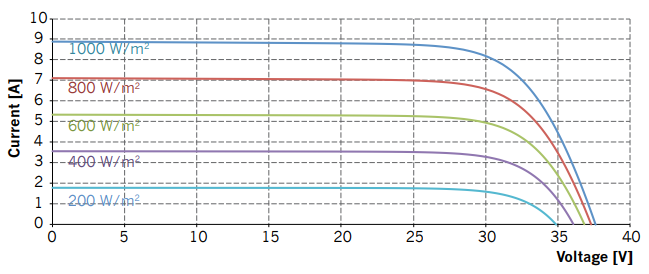
\includegraphics[width=10cm]{imagenes/VIpaneles}
	\caption{V-I Curva de diferentes niveles de irradiancia \cite{DDE1}.}
	\label{fig:VIcurva}
\end{figure}

Es importante mencionar que la eficiencia de los paneles no es del 100\%, debido a que se producen pérdidas por diferentes factores como la temperatura, la suciedad, el tiempo de funcionamiento, entre otros. Para determinar la cantidad de potencia real necesaria se utilizó índice de rendimiento de 0.9, con el fin de contrarrestar las pérdidas que pudieran generarse \cite{DDE2}. Dicho cálculo se realiza mediante la ecuación (\ref{eq:eec1}).\\
\begin{equation}\label{eq:eec1}
P_{nec} = \frac{P_{ideal\_arreglo}}{\eta} 
\end{equation}

Donde $P_{nec}$ es la potencia real para contrarrestar las pérdidas de los paneles, $P_{ideal\_arreglo}$ es la potencia ideal mínima a generar, y $\eta$ es el índice de rendimiento de los paneles. Dado que $P_{ideal\_arreglo}$=1000 W y sustituyendo en (\ref{eq:eec1}), se obtuvo la Ecuación (\ref{eq:ec1sust}): 
\begin{equation}\label{eq:ec1sust}
P_{nec} = \frac{1000 \ W}{0.9} = 1111.11 \ W
\end{equation}

Conociendo el valor de potencia necesaria que deberán generar los paneles, se prosiguió a calcular el número mínimo de paneles. Para obtener este valor se utilizó la Ecuación (\ref{eq:ec2}):
\begin{equation}\label{eq:ec2}
N_{paneles} = \frac{P_{nec}}{P_{max\_panel}} 
\end{equation}

Donde $N_{paneles}$ es el número mínimo de paneles para generar la potencia real necesaria, y $P_{max\_panel}$ es la potencia máxima de cada panel. Sustituyendo en (\ref{eq:ec2}), se obtuvo el valor mostrado en la Ecuación (\ref{eq:ec2sust}):
\begin{equation}\label{eq:ec2sust}
N_{paneles} = \frac{1111.11 \ W}{255 \ W} = 4.35 \approx 5 
\end{equation}

Con el resultado anterior, se puede deducir que para generar al menos 1 kWh de energía, se necesitan como mínimo 5 paneles de 255 W.\\ 

Al diseñarse una estructura capaz de aguantar hasta 12 paneles de 255 W cada uno, se calculó la potencia real que estos pueden generar. Para ello, se despejó de (\ref{eq:ec2}) la potencia necesaria \textbf{\textit{$P_{nec}$}}, obteniendo la Ecuación (\ref{eq:ec3}):
\begin{equation}\label{eq:ec3}
P_{nec} = N_{paneles} \times P_{max\_panel}
\end{equation}

Sustituyendo los valores conocidos en la ecuación anterior, se obtuvo la Ecuación (\ref{eq:ec3sust}):
\begin{equation}\label{eq:ec3sust}
P_{nec} = 12 \times 255 \ W = 3060 \ W
\end{equation}

Habiendo obtenido el valor de la potencia necesaria, se prosiguió a calcular el valor de la potencia real generada por el sistema, $P_{real_arreglo}$, la cual se obtuvo despejándola de (\ref{eq:eec1}), teniendo como resultado la Ecuación (\ref{eq:ec4}).
\begin{equation}\label{eq:ec4}
P_{real\_arreglo} = P_{nec}  \times  \eta
\end{equation}

Sustituyendo los valores en la Ecuación (\ref{eq:ec4}), se obtuvo lo siguiente:
\begin{equation}\label{eq:ec4sust}
P_{real\_arreglo} = 3060 \ W \times 0.9 = 2754 \ W
\end{equation}

Obteniendo así una potencia real generada por los 12 paneles de \textbf{2754 W}.\\

Conociendo la cantidad total de paneles, se determinó el número de ellos que son necesarios conectar en serie. Para esto, se seleccionó la tensión nominal del sistema con base a la potencia demandada por este. Esta selección se hizo con base en la Tabla \ref{tab:Tensionnom}, la cual muestra el valor de tensión nominal recomendado según la potencia demandada.

\begin{table}[H]
	\centering
	\caption{Tensión nominal de la instalación en función de la potencia demandada \cite{DDE2}.}
	\begin{tabular}{|l|c|}
		\hline
		\multicolumn{1}{|p{10.57em}|}{\textbf{Potencia demandada}} & \multicolumn{1}{p{12.285em}|}{\textbf{Tensión nominal de la instalación}} \\
		\hline
		P < 1500 W & 12 V \\
		\hline
		1500 W $\leq$ P $\leq$ 5000 W & 24 V, 48 V \\
		\hline
		P > 5000 W & 48 V, 120 V \\
		\hline
	\end{tabular}%
	\label{tab:Tensionnom}%
\end{table}%

Al tener una potencia necesaria de 3060 W, se optó por seleccionar una \textbf{tensión nominal de 48 V}. Habiendo establecido el valor de tensión nominal, se prosiguió a calcular el número de paneles conectados en serie, esto mediante la Ecuación (\ref{eq:ec5}).
\begin{equation}\label{eq:ec5}
NP_{s} = \frac{V_{ns}}{V_{np}} 
\end{equation}

Donde $NP_{s}$ es el número de paneles solares conectados en serie, $V_{ns}$ es la tensión nominal de la instalación, y $V_{np}$ es la tensión nominal de los paneles solares. Sustituyendo los valores en (\ref{eq:ec5}), se obtuvo la Ecuación (\ref{eq:ec5sust}):
\begin{equation}\label{eq:ec5sust}
NP_{s} = \frac{48 V}{24 V}=2 
\end{equation}

Una vez calculado el número de paneles conectados en serie, se obtuvo el número de paneles conectados en paralelo con la Ecuación (\ref{eq:ec6}):
\begin{equation}\label{eq:ec6}
NP_{p} =\frac{P_{req}}{NP_{s} \times P_{max\_panel}} 
\end{equation}

Donde $NP_{p}$ es el número de paneles solares conectados en paralelo, y $P_{nec}$ es la potencia requerida total del arreglo. Sustituyendo los valores en la Ecuación (\ref{eq:ec6}), se obtuvo:
\begin{equation}\label{eq:ec6sust}
NP_{p} = \frac{3060 \ W}{2 \times 255 \ W}=6 
\end{equation}

Conociendo el número de paneles que se tendrán que conectar, se calculó la cantidad total de paneles requerida para todo el arreglo, mediante la Ecuación (\ref{eq:ec7}): 
\begin{equation}\label{eq:ec7}
NP_{t} = NP_{p} \times NP_{s}  
\end{equation}
Donde $NP_{t}$ es el número total de paneles solares conectados en serie y paralelo. Sustituyendo en (\ref{eq:ec7}), se obtuvo la Ecuación (\ref{eq:ec7sust}):
\begin{equation}\label{eq:ec7sust}
NP_{t} = 6 \times 2 = 12  
\end{equation}

Se puede observar que coincide con la cantidad de paneles que la estructura deberá de soportar. En la Figura \ref{fig:Dispan} se muestran las conexiones entre ellos:
\begin{figure}[H]
	\centering
	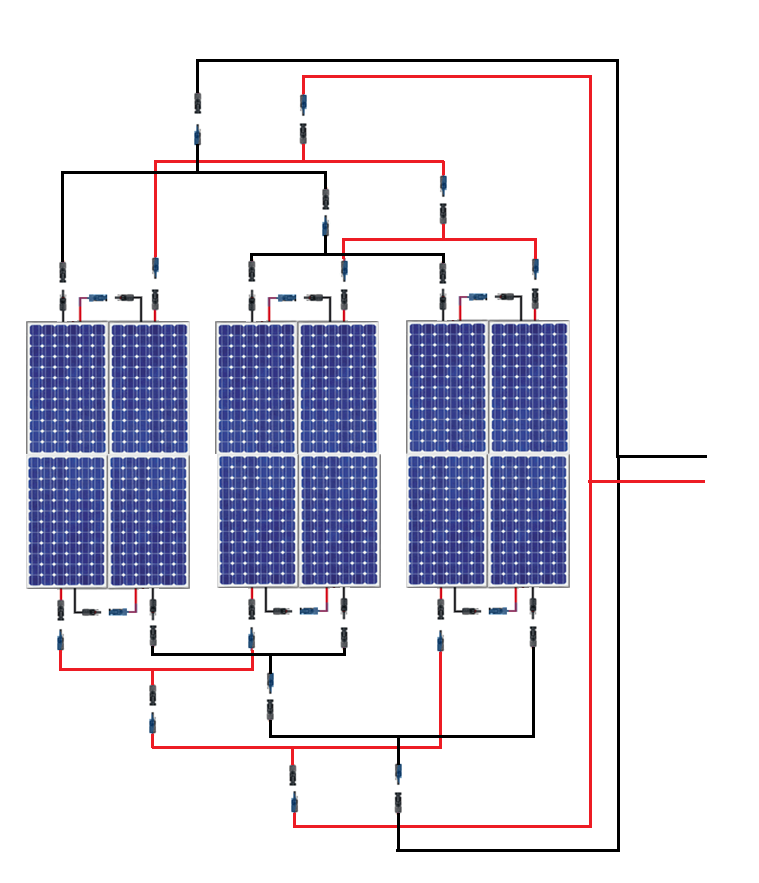
\includegraphics[width=7cm]{imagenes/Dispan}
	\caption{Conexión paneles solares.}
	\label{fig:Dispan}
\end{figure}

\subsubsection{Cálculo y selección del medio de almacenamiento} \label{sec:baterias}
Para este cálculo se tomó el valor de potencia real del arreglo de paneles calculado anteriormente, haciendo uso de la Ecuación (\ref{eq:ec8}) \cite{DDE2}: 
\begin{equation}\label{eq:ec8}
E = P_{real_arreglo} \times HSP   
\end{equation}

Donde \textbf{E} es la energía generada en Wh, y \textbf{HSP} es el tiempo equivalente medido en horas solar pico, obtenido de la irradiación recibida durante el periodo de tiempo considerado.\\

Para definir el número de horas que el sistema generará energía se utilizó la Tabla \ref{tab:irra}, donde se muestran las horas solares pico mensuales para la ubicación definida en los requerimientos.  

\begin{table}[H]
	\centering
	\caption{Irradiancia solar óptima mensual \cite{DDE3}.}
	\begin{tabular}{|p{1.4em}|p{1.3em}|p{1.7em}|p{1.7em}|p{1.7em}|p{1.5em}|p{1.3em}|p{1.7em}|p{1.5em}|p{1.5em}|p{1.7em}|p{1.5em}|p{2.7em}|}
		\hline
		\textbf{Ene} & \textbf{Feb} & \textbf{Mar} & \textbf{Abr} & \textbf{May} & \textbf{Jun} & \textbf{Jul} & \textbf{Ago} & \textbf{Sep} & \textbf{Oct} & \textbf{Nov} & \textbf{Dic} & \textbf{Anual} \\
		\hline
		6.3   & 6.4   & \cellcolor[rgb]{ 1,  .2,  .6}6.87 & 6.41  & 6.2   & 5.63  & 5.52  & 5.29  & \cellcolor[rgb]{ .2,  .4,  1}5 & 5.37  & 6.08  & 5.77  & 5.91 \\
		\hline
	\end{tabular}%
	\label{tab:irra}%
\end{table}%

\begin{table}[H]
	\begin{tabular}{cl}
		\rowcolor[rgb]{ 1,  .2,  .6}       & \cellcolor[rgb]{ 1,  1,  1}Horas solar pico (HSP) máximas en el año. \\
		&  \\
		\rowcolor[rgb]{ .2,  .4,  1}       & \cellcolor[rgb]{ 1,  1,  1}Horas solar pico (HSP) mínimas en el año. \\
	\end{tabular}%
\end{table}%

Se tomó el valor máximo de horas que se puede tener a lo largo del año, siendo de \textbf{6.87 horas}, para considerar el caso en que el sistema tendrá que soportar la máxima cantidad de irradiancia, definiendo este valor como el número máximo de horas que se almacenará energía durante el día, evitando alguna sobrecarga. Para realizar el cálculo de la energía máxima generada durante un día se sustituyeron los valores en la Ecuación (\ref{eq:ec8}) y se obtuvo: 
\begin{equation}\label{eq:ec8sust}
E = 2754 \ W \times 6.87 \ h \approx 18.92 \ kWh   
\end{equation}

Sabiendo que en un sistema fotovoltaico autónomo existen factores que provocan perdidas en el rendimiento global, se definió un nuevo valor dado por la Ecuación (\ref{eq:ec9}) \cite{DDE4}: 
\begin{equation}\label{eq:ec9}
E_{t} = \frac{E}{R}   
\end{equation}

Donde $E_{t}$ es la energía necesaria a generar considerando las pérdidas del sistema global, y \textbf{R} es el rendimiento global del sistema.\\

Para el cálculo de R es necesario considerar los siquientes parámetros de diseño \cite{DDE4}:

\textbf{Ka: Coeficiente de pérdidas por autodescarga de las baterías.}\\
\hspace*{4em} 0.02 para baterías Niquel-Cadmio.\\
\hspace*{4em} 0.005 para baterías estacionarias de Plomo-Ácido.\\

\textbf{Kb: Coeficiente de pérdidas por rendimiento de las baterías.} Índica la fracción de energía que la batería no devuelve con respecto a la absorbida procedente de los paneles. \\
\hspace*{4em}0.05 para sistemas donde no se generan descargas intensas \\
\hspace*{4em}0.1 sistemas donde se generan descargas intensas\\

\textbf{Kc: Coeficiente de pérdidas por rendimiento del inversor.} Afectará el rendimiento global de la instalación en caso de que el consumo se realice en alterna mediante inversor. \\
\hspace*{4em}0.005 Inversores de onda senoidal pura\\
\hspace*{4em}0.1 inversores de onda senoidal\\
\hspace*{4em}0.4 inversores de onda cuadrada\\

En instalaciones autónomas, para el cálculo del subsistema acumulador, este coeficiente es 0, pues no existe ningún inversor previo desde el subsistema generador. \\

\textbf{Kv: Coeficiente de pérdidas varias.} Este coeficiente tiene en cuenta el rendimiento global de toda la red de consumo, perdidas por efecto Joule, etc.\\
\hspace*{4em}Este coeficiente adopta valores entre 0.05 y 0.15\\

Otro factor que va a influir en el rendimiento de la instalación es: \\
\textbf{Pd: Profundidad de descarga de las baterías}\\
\hspace*{4em}Con valores entre el 50\%  y el 80\%.\\
\textbf{N: Número de días de autonomía de la instalación.} Número de días sin radiación solar que pueden estar funcionando las cargas en condiciones normales. \\
\hspace*{4em}Con valores de 2 a 8 días. \\

Así, el rendimiento global $R$ de la instalación se calcula mediante la Ecuación (\ref{eq:ec10}):
\begin{equation}\label{eq:ec10}
R = (1-K_{b}-K_{c}-K_{v}) (1-K_{a} (\frac{N}{Pd})) 
\end{equation}

Para el cálculo de R se definieron los siguientes valores para cada uno de los coeficientes: 

\hspace*{2.5em}\textbf{Ka=0.005}, al ser el tipo de baterías que genera menores pérdidas.\\
\hspace*{4em}\textbf{Kb=0.1}, caso crítico, donde el sistema estaría sometido a descargas intensas.\\
\hspace*{4em}\textbf{Kc=0}, al tratarse de un sistema autónomo.\\
\hspace*{4em}\textbf{Kv=0.15}, considerando el valor máximo de pérdidas por rendimiento.\\
\hspace*{4em}\textbf{Pd=0.6}, considerando un valor de 0.6 de profundidad de descarga.\\
\hspace*{4em}\textbf{N=2 días}, proponiendo 2 días de autonomía de la instalación.\\

Al sustituir estos valores en (\ref{eq:ec10}) , se obtuvo la Ecuación (\ref{eq:ec10sust}): 
\begin{equation}\label{eq:ec10sust}
R = (1-0.1-0-0.5) (1-0.005 (\frac{2}{0.6}))=0.7375 
\end{equation}

Por medio de la Ecuación (\ref{eq:ec9}) se obtuvo la energía necesaria considerando las perdidas.
\begin{equation}\label{eq:ec9sust}
E_{t} = \frac{18.92 \ kWh}{0.7375}=25654.23 \ Wh   
\end{equation}

Una vez calculada la energía necesaria a generar y fijado el número de días de autonomía \textit{\textbf{N}}, se determinó la capacidad útil, \textbf{$C_{u}$}, de las baterías, entendida como la capacidad que se extraerá de las mismas, con la Ecuación (\ref{eq:ec11}): 
\begin{equation}\label{eq:ec11}
C_{u} = E_{t} \times N   
\end{equation}
\begin{equation}\label{eq:ec11sust}
C_{u} =25654.23 \ W \times 2 = 51308.47 \ Wh   
\end{equation}

\textbf{$C_{n}$} tendrá que ser mayor que la capacidad útil, ya que solo deberá descargarse hasta la profundidad de descarga establecida, \textit{\textbf{Pd}}. Así, La capacidad nominal de la batería corresponde a la Ecuación(\ref{eq:ec12}) y su cálculo a la Ecuación (\ref{eq:ec12sust}). 
\begin{equation}\label{eq:ec12}
C_{n} = \frac{C_{u}}{Pd}
\end{equation}
\begin{equation}\label{eq:ec12sust}
C_{n} = \frac{51308.47 \ Wh}{0.6}=85514.12 \ Wh
\end{equation}

Comercialmente los valores de capacidad de una batería $(C_{n_ah})$ están en Ah, así que el resultado anterior se dividió entre la tensión nominal del sistema para convertirlo a dicha unidad, empleando las Ecuaciones (\ref{eq:ec13}) y (\ref{eq:ec13sust}):
\begin{equation}\label{eq:ec13}
C_{n_ah} = \frac{C_{n}}{V_{ns}}
\end{equation}
\begin{equation}\label{eq:ec13sust}
C_{n_ah} = \frac{85514.12 \ Wh}{48 \ V}=1781.54 \ Ah
\end{equation}

Conociendo la capacidad de las baterías, se elaboró el árbol de decisión mostrado en la Figura \ref{fig:Arrutbat}, el cual permitió reducir el número posible de soluciones de 62 a solo 3.\\
\begin{figure}[H]
	\centering
	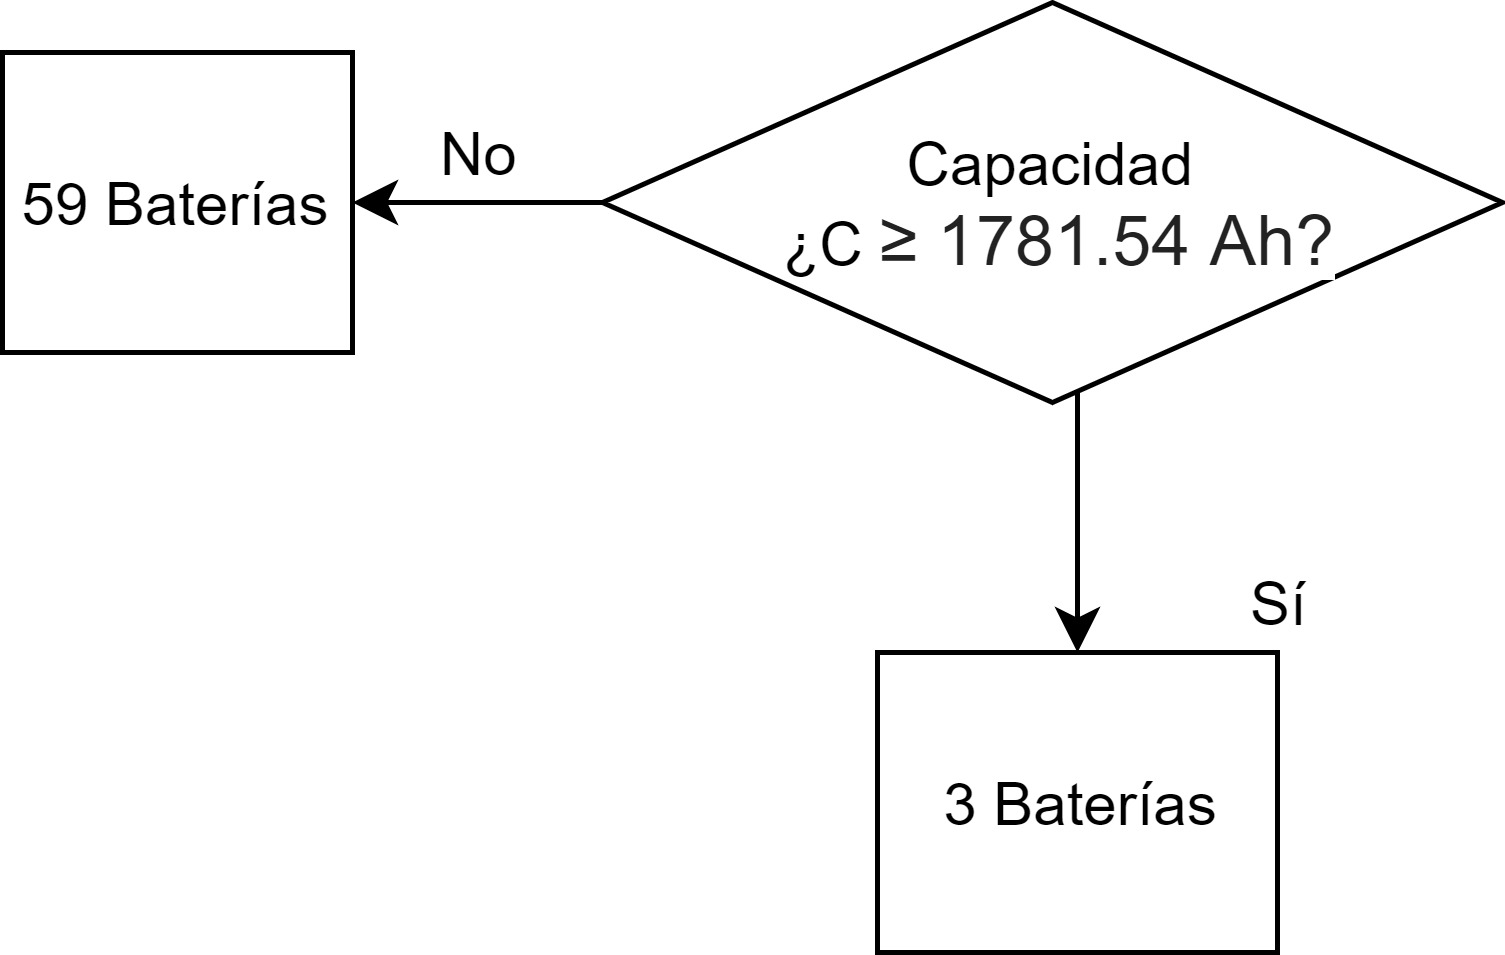
\includegraphics[width=7cm]{imagenes/Arrutabat}
	\caption{Árbol de decisiones baterías almacenamiento total.}
	\label{fig:Arrutbat}
\end{figure}

Se prosiguió a realizar la selección por medio de un método multicriterio, es este caso AHP, definiendo los siguientes criterios para la selección:\\
\hspace*{4em}\textit{Cr1.} Capacidad.\\
\hspace*{4em}\textit{Cr2.} Dimensiones.\\
\hspace*{4em}\textit{Cr3.} Costo.\\
\hspace*{4em}\textit{Cr4.} Tipo.\\
\hspace*{4em}\textit{Cr5.} Peso.\\
Una vez, establecidos los criterios, se obtuvo de resultado mostrado en la Tabla \ref{tab:mm1}:

\begin{table}[H]
	\centering
	\caption{Evaluación de criterios para las baterías que almacenarán toda la energía.}
	\begin{tabular}{|c|c|c|c|c|c|c|}
		\hline  
		\multicolumn{1}{|r|}{} & \cellcolor[rgb]{ .741,  .839,  .933}Cr1 & \cellcolor[rgb]{ .741,  .839,  .933}Cr2 & \cellcolor[rgb]{ .741,  .839,  .933}Cr3 & \cellcolor[rgb]{ .741,  .839,  .933}Cr4 & \cellcolor[rgb]{ .741,  .839,  .933}Cr5 & \cellcolor[rgb]{ .741,  .839,  .933}VALOR FINAL \\
		\hline
		\rowcolor[rgb]{ .659,  .816,  .553} PB1   & \cellcolor[rgb]{ 1,  .753,  0}0.07830782 & \cellcolor[rgb]{ 1,  .753,  0}0.1886372 & \cellcolor[rgb]{ 1,  .753,  0}0.10051976 & \cellcolor[rgb]{ 1,  .753,  0}0.01723848 & \cellcolor[rgb]{ 1,  .753,  0}0.06440482 & \cellcolor[rgb]{ 1,  .753,  0}0.449108086 \\
		\hline
		\rowcolor[rgb]{ .659,  .816,  .553} PB2   & \cellcolor[rgb]{ 1,  1,  1}0.13623814 & \cellcolor[rgb]{ 1,  1,  1}0.10842608 & \cellcolor[rgb]{ 1,  1,  1}0.057777383 & \cellcolor[rgb]{ 1,  1,  1}0.03447696 & \cellcolor[rgb]{ 1,  1,  1}0.06440482 & \cellcolor[rgb]{ 1,  1,  1}0.401323395 \\
		\hline
		\rowcolor[rgb]{ .659,  .816,  .553} PB3   & \cellcolor[rgb]{ 1,  1,  1}0.02998404 & \cellcolor[rgb]{ 1,  1,  1}0.04151631 & \cellcolor[rgb]{ 1,  1,  1}0.022122939 & \cellcolor[rgb]{ 1,  1,  1}0.03447696 & \cellcolor[rgb]{ 1,  1,  1}0.02146827 & \cellcolor[rgb]{ 1,  1,  1}0.149568518 \\
		\hline
	\end{tabular}%
	\label{tab:mm1}%
\end{table}

La propuesta de baterías ganadora fue la primera, cuyas características son:

\hspace*{1em}\textbf{\textit{Marca:}} Surrette Rolls.\\
\hspace*{2.5em}\textbf{\textit{Tipo:}} Sellada.\\
\hspace*{2.5em}\textbf{\textit{Modelo:}} 2-YS-31PS.\\
\hspace*{2.5em}\textbf{\textit{Tensión nominal:}} 2 V. \\
\hspace*{2.5em}\textbf{\textit{Capacidad:}} 2430 Ah (C20).\\
\hspace*{2.5em}\textbf{\textit{Dimensiones:}} 15.5 x 9.25 x 31.625 in.\\
\hspace*{2.5em}\textbf{\textit{Peso:}} 285 lb.\\
\hspace*{2.5em}\textbf{\textit{Precio:}} \$1,218.00 (US).\\

Para calcular el número de baterías conectadas en serie, se utilizó la Ecuación (\ref{eq:ec14}):
\begin{equation}\label{eq:ec14}
NB_{s} = \frac{V_{ns}}{V_{nb}}
\end{equation}

Donde $NB_{s}$ es el número de baterías conectadas en serie, y $V_{nb}$ es la tensión nominal de las baterías seleccionadas. Sustituyendo los valores en la Ecuación (\ref{eq:ec14}), queda los siguiente:
\begin{equation}\label{eq:ec14sust}
NB_{s} = \frac{48 \ V}{2 \ V}=24
\end{equation}

Para calcular el número de baterías conectadas en paralelo, se empleó la Ecuación (\ref{eq:ec15}):
\begin{equation}\label{eq:ec15}
NB_{p} = \frac{C_{n}}{C_{p}}
\end{equation}

Donde $NB_{p}$ es el número de baterías conectadas en paralelo, $C_{n}$ es la capacidad necesaria del sistema, y $C_{b}$ es la capacidad de las baterías. Sustituyendo en la Ecuación (\ref{eq:ec15}), se obtiene la Ecuación \ref{eq:ec15sust}.
\begin{equation}\label{eq:ec15sust}
NB_{p} = \frac{1781.54  \ Ah}{2430 \ Ah}=0.733 \approx 1
\end{equation}

El número total de baterías se calcula con la Ecuación (\ref{eq:ec16}), obteniendo la Ecuación \ref{eq:ec16sust} al sustituir valores.
\begin{equation}\label{eq:ec16}
NB_{t} = NB_{p} \times NB_{s}
\end{equation}
\begin{equation}\label{eq:ec16sust}
NB_{t} = 1 \times 24=24
\end{equation}

Se necesitan 24 baterías $ 2-YS-31PS $ para el almacenamiento de toda la energía, por lo que se realizó el cálculo del costo total de las baterías, obteniendo que:
\begin{equation}\label{eq:CostoBaterias}
    Costo\ bater\'ias\ =\ 24\ bater\'ias\ \times\ \$1,218.00=\$29,232.00\ (US)
\end{equation}

Almacenar toda la energía resultaría costoso, además de requerir un espacio considerable, así que se optó por almacenar únicamente la energía que el seguidor solar consumiría. Según \cite{DDE5}, un seguidor solar debe consumir entre el 2\% y el 3\% de la energía generada, así que se calculó el 3\% de la energía que el seguidor debe generar al día, teniendo como resultado:
\begin{equation}\label{eq:ec19}
E_{seguidor} = E \times 0.03
\end{equation}
\begin{equation}\label{eq:ec20}
E_{seguidor} = 18.92 \ kW \times 0.03=567.6 \ Wh
\end{equation}

Partiendo de este valor, se utilizaron las Ecuaciones (\ref{eq:ec19}) y (\ref{eq:ec20}) para calcular la capacidad del medio de almacenamiento.
\begin{equation}\label{eq:ec9sust1}
E_{t} = \frac{567.3 \ Wh}{0.7375}=769.62 \ Wh
\end{equation}
\begin{equation}\label{eq:ec11sust1}
C_{u} =769.62 \ Wh \times 2 = 1539.25 \ Wh
\end{equation}
\begin{equation}
C_{n} = \frac{1539.25 \ Wh}{0.6}=2565.42 \ Wh
\end{equation}
\begin{equation}\label{eq:ec21}
C_{n_ah} = \frac{2565.42 \ Wh}{48 \ V}=53.44 \ Ah
\end{equation}

Para la selección de la batería se elaboró un árbol de decisión, con el fin de disminuir el número de posibles soluciones, el cual se muestra en la Figura \ref{fig:Arrutbat2}. 
\begin{figure}[H]
	\centering
	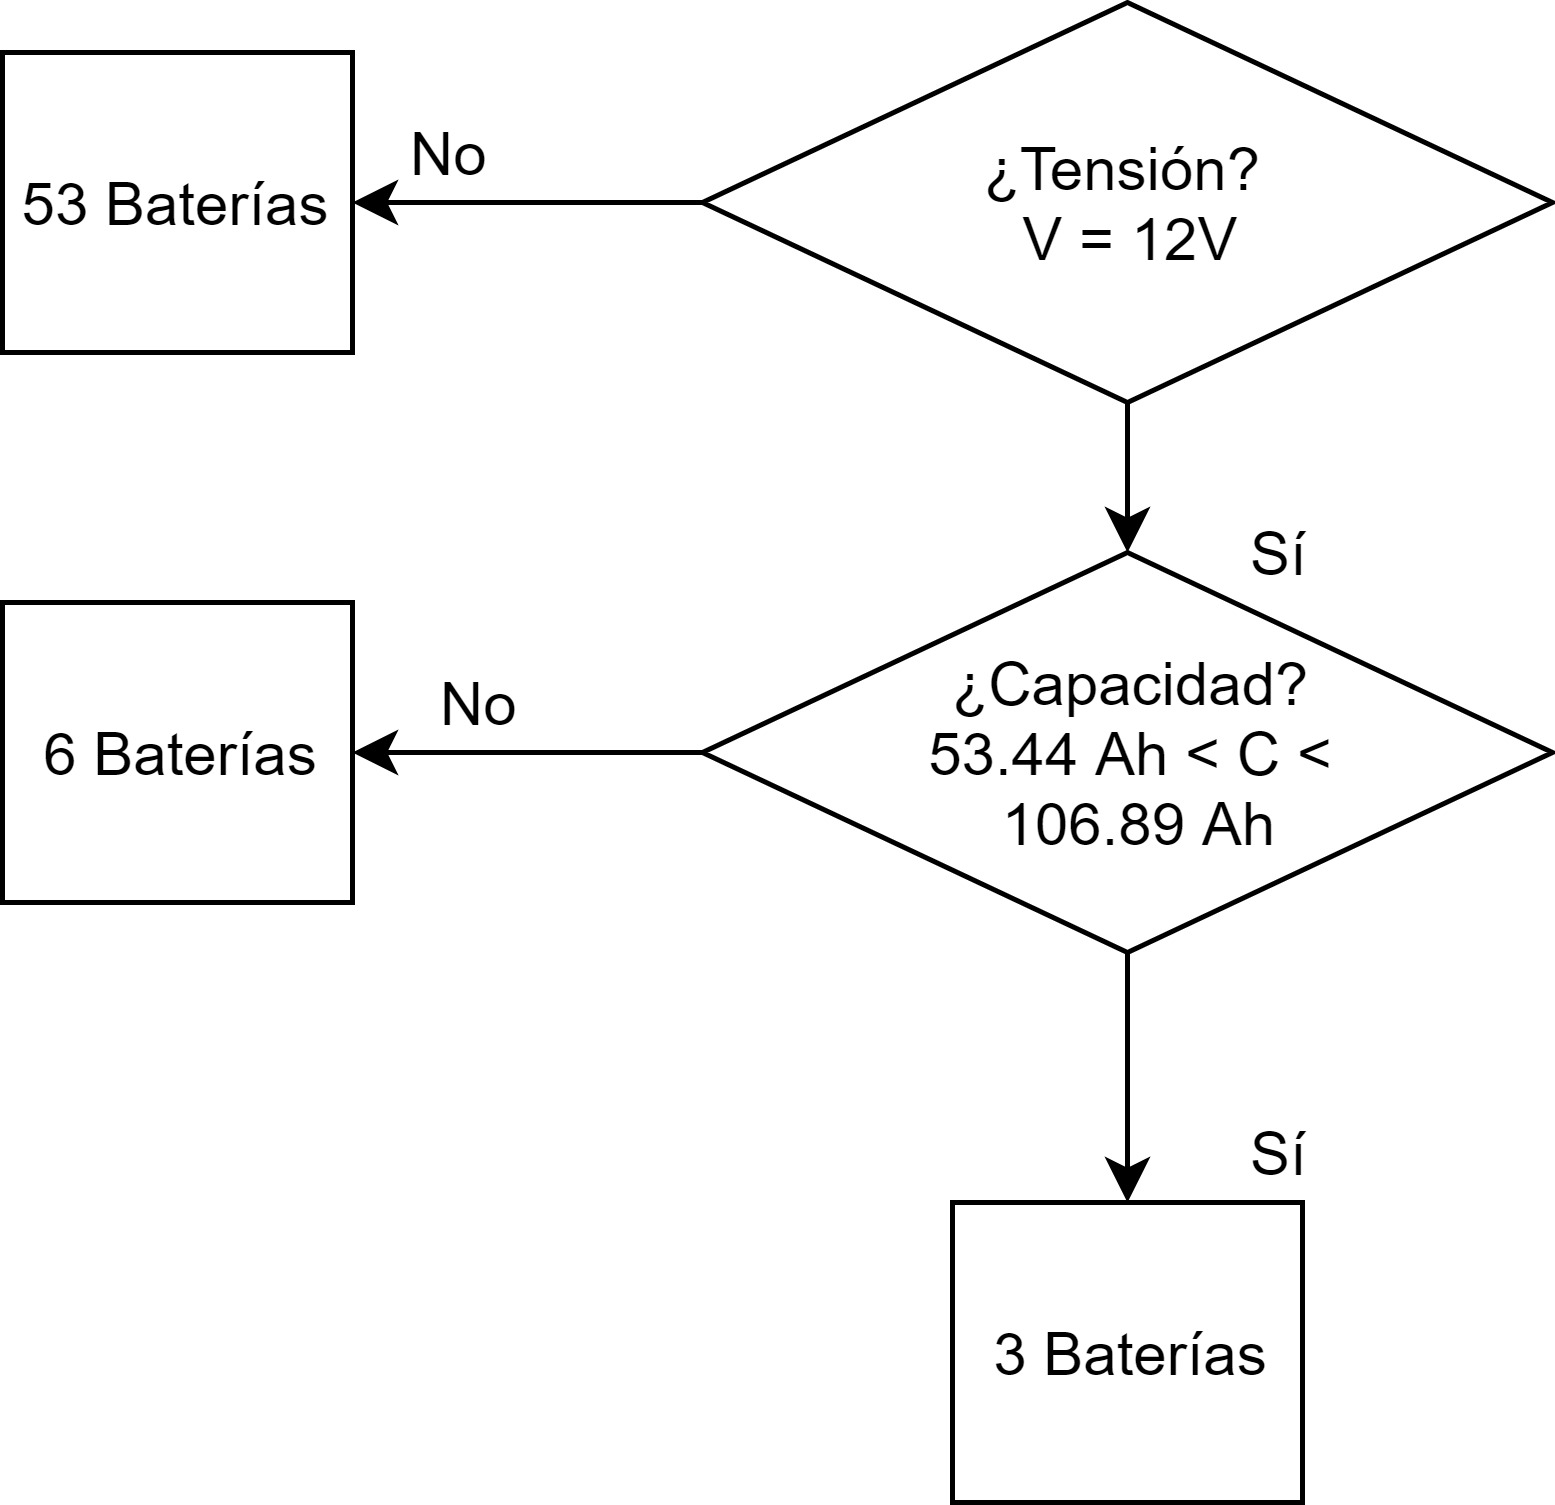
\includegraphics[width=7cm]{imagenes/Arrutabat2}
	\caption{Árbol de decisiones baterías almacenamiento 3\%.}
	\label{fig:Arrutbat2}
\end{figure}

Se obtuvieron 3 posibles soluciones de 62 del árbol de decisión. Se prosiguió a realizar la selección por medio de una herramienta multicriterio, utilizando los criterios ya establecidos. obteniendo los resultados mostrados en la Tabla \ref{tab:addlabel1}:
\begin{table}[H]
	\centering
	\caption{Evaluación de criterios para las baterías que almacenarán el 3\% de energía.}
	\begin{tabular}{|c|c|c|c|c|c|c|}
		\hline    
		\multicolumn{1}{|r|}{} & \cellcolor[rgb]{ .612,  .761,  .898}Cr1 & \cellcolor[rgb]{ .612,  .761,  .898}Cr2 & \cellcolor[rgb]{ .612,  .761,  .898}Cr3 & \cellcolor[rgb]{ .612,  .761,  .898}Cr4 & \cellcolor[rgb]{ .612,  .761,  .898}Cr5 & \cellcolor[rgb]{ .612,  .761,  .898}Suma \\
		\hline 
		\rowcolor[rgb]{ .659,  .816,  .553} PB1   & \cellcolor[rgb]{ 1,  1,  1}0.097812 & \cellcolor[rgb]{ 1,  1,  1}0.06771592 & \cellcolor[rgb]{ 1,  1,  1}0.10051976 & \cellcolor[rgb]{ 1,  1,  1}0.01723848 & \cellcolor[rgb]{ 1,  1,  1}0.08099394 & \cellcolor[rgb]{ 1,  1,  1}0.3642801 \\
		\hline
		\rowcolor[rgb]{ .659,  .816,  .553} PB2   & \cellcolor[rgb]{ 1,  1,  1}0.048906 & \cellcolor[rgb]{ 1,  1,  1}0.06771592 & \cellcolor[rgb]{ 1,  1,  1}0.05777738 & \cellcolor[rgb]{ 1,  1,  1}0.01723848 & \cellcolor[rgb]{ 1,  1,  1}0.04467136 & \cellcolor[rgb]{ 1,  1,  1}0.23630914 \\
		\hline
		\rowcolor[rgb]{ .659,  .816,  .553} PB3   & \cellcolor[rgb]{ 1,  .753,  0}0.097812 & \cellcolor[rgb]{ 1,  .753,  0}0.20314776 & \cellcolor[rgb]{ 1,  .753,  0}0.02212294 & \cellcolor[rgb]{ 1,  .753,  0}0.05171544 & \cellcolor[rgb]{ 1,  .753,  0}0.02461262 & \cellcolor[rgb]{ 1,  .753,  0}0.39941076 \\
		\hline
	\end{tabular}%
	\label{tab:addlabel1}%
\end{table}%

La propuesta de baterías ganadora fue la tercera, cuyas características son:

\hspace*{1em}\textbf{\textit{Marca:}} Full River.\\
\hspace*{2.5em}\textbf{\textit{Tipo:}} Sellada.\\
\hspace*{2.5em}\textbf{\textit{Modelo:}} DC85-12.\\
\hspace*{2.5em}\textbf{\textit{Tensión nominal:}} 12 V.\\ 
\hspace*{2.5em}\textbf{\textit{Capacidad:}} 85 Ah (C20).\\
\hspace*{2.5em}\textbf{\textit{Dimensiones:}} 10.25 x 6.75 x 8.5 in.\\
\hspace*{2.5em}\textbf{\textit{Peso:}} 55 lb.\\
\hspace*{2.5em}\textbf{\textit{Precio:}} \$222.00 (US).\\

Para calcular el número de baterías se hizo uso de las Ecuaciones (\ref{eq:ec14}), (\ref{eq:ec15}) y (\ref{eq:ec16}), obteniendo los siguientes resultados:
\begin{equation}\label{eq:ec22}
NB_{s} = \frac{48 \ V}{12 \ V}=4
\end{equation}
\begin{equation}\label{eq:ec23}
NB_{p} = \frac{53.54 \ Ah}{85 \ Ah}=0.0.62 \approx 1
\end{equation}
\begin{equation}\label{eq:ec24}
NB_{t} = 1 \times 4 = 4
\end{equation}

Con esto se concluye que se necesitan 4 baterías $ DC85-12 $ para el almacenamiento de la energía que el seguidor consumirá.
\begin{figure}[H]
	\centering
	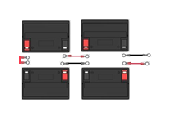
\includegraphics[width=5cm]{imagenes/Confbat1.eps}
	\caption{Conexión de baterías.}
	\label{fig:Confbat}
\end{figure}

Realizando el cálculo del costo de las baterías se obtuvo que:
\begin{equation}\label{eq:ec25}
Costo\; baterias = 4\; baterias \times \$222.00 =\$888.00 (US)
\end{equation}

Como se puede ver, el costo reduce en gran medida a comparación del primer cálculo, donde se consideró almacenar toda la cantidad de energía generada.

\subsubsection{Cálculo y selección del regulador}

Para determinar las características eléctricas del regulador es necesario conocer la intensidad pico generada por el panel solar, \textit{$I_g$}, la intensidad total del consumo \textit{$I_c$}, y la potencia \textit{$P_{req}$} requerida. Inicialmente se calculó \textit{$I_g$}, partiendo de la intensidad pico del panel solar elegido \textit{$I_p$}, siendo su valor la intensidad de corto circuito \textit{$I_{sc}$} del panel, aumentada en un 25\% \cite{DDE6} para tener en cuenta temperatura e irradiancia superiores a los valores STC de ensayo (25 °C y 1000 W/m2), de modo que: 
\begin{equation}\label{eq:ec26}
I_{g} = 1.25 \times NP_{p} \times I_{p}
\end{equation}
\begin{equation}\label{eq:ec27}
I_{g} = 1.25 \times 6 \times 8.93 \ A=53.58 \ A
\end{equation}

El cálculo de la intensidad de consumo, \textit{$I_c$}, se hizo utilizando la Ecuación (\ref{eq:ec28}), considerando que si se quisiera colocar un inversor, iría conectado a la batería, siendo innecesario que este incluya entre sus funciones la protección contra la descarga excesiva de la batería, reduciendo así la intensidad que debe suministrar el inversor.
\begin{equation}\label{eq:ec28}
I_{c} = P_{nec} \times V_{ns}
\end{equation}
\begin{equation}\label{eq:ec28sust}
I_{c} = 3000 \ W \times 48 V=62.5 \ A
\end{equation}

Por lo tanto, las corrientes máximas de entrada y salida del regulador son \textbf{53.58 A y 62.5 A}, respectivamente.
\begin{figure}[H]
	\centering
	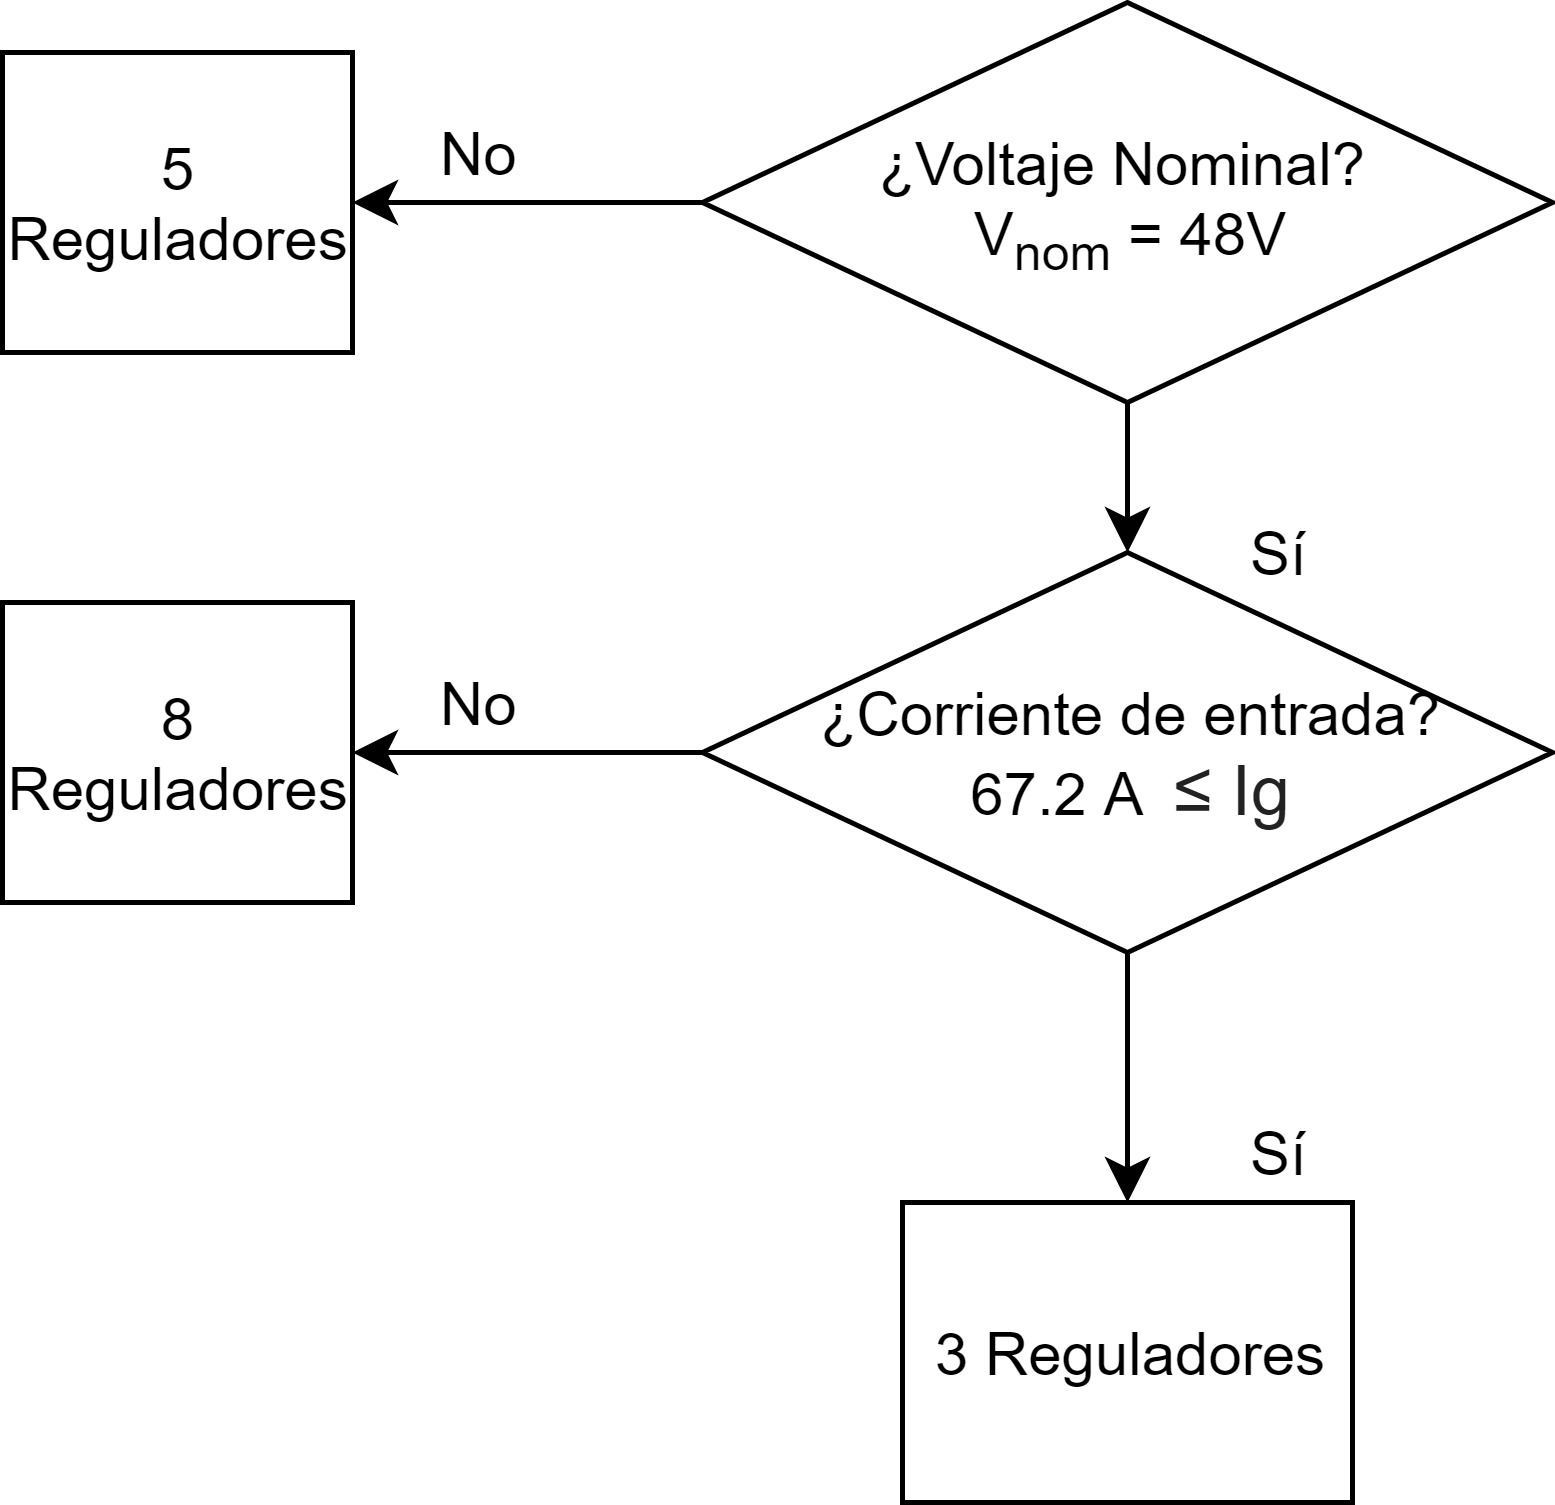
\includegraphics[width=7cm]{imagenes/Arrutareg}
	\caption{Árbol de decisiones para el regulador.}
	\label{fig:Arrutareg}
\end{figure}

Se obtuvieron 3 posibles soluciones de 16, producto del árbol de decisión de la Figura \ref{fig:Arrutareg}. Como siguiente paso, se prosiguió a realizar la selección por medio de un método multicriterio, es este caso AHP, definiendo los siguientes criterios:\\
\textbf{\textit{Cr1.}} Consumo energético.\\
\textbf{\textit{Cr2.}} Dimensiones.\\
\textbf{\textit{Cr3.}} Costo.\\
\textbf{\textit{Cr4. }}Peso. \\
\textbf{\textit{Cr5.}} Corriente nominal.\\

Con los criterios establecidos, se obtuvo como resultado la siguiente matriz:
\begin{table}[H]
	\centering
	\caption{Evaluación de criterios para la selección del regulador.}
	\begin{tabular}{|c|c|c|c|c|c|c|}
		\hline   
		\multicolumn{1}{|r|}{} & \cellcolor[rgb]{ .612,  .761,  .898}Cr1 & \cellcolor[rgb]{ .612,  .761,  .898}Cr2 & \cellcolor[rgb]{ .612,  .761,  .898}Cr3 & \cellcolor[rgb]{ .612,  .761,  .898}Cr4 & \cellcolor[rgb]{ .612,  .761,  .898}Cr5 & \cellcolor[rgb]{ .612,  .761,  .898}Total \\
		\hline
		\rowcolor[rgb]{ .659,  .816,  .553} PB1   & \cellcolor[rgb]{ 1,  .753,  0}0.11819477 & \cellcolor[rgb]{ 1,  .753,  0}0.02819162 & \cellcolor[rgb]{ 1,  .753,  0}0.09290525 & \cellcolor[rgb]{ 1,  .753,  0}0.05920945 & \cellcolor[rgb]{ 1,  .753,  0}0.12250644 & \cellcolor[rgb]{ 1,  .753,  0}0.42100754 \\
		\hline
		\rowcolor[rgb]{ .659,  .816,  .553} PB2   & \cellcolor[rgb]{ 1,  1,  1}0.05815933 & \cellcolor[rgb]{ 1,  1,  1}0.01377135 & \cellcolor[rgb]{ 1,  1,  1}0.05910062 & \cellcolor[rgb]{ 1,  1,  1}0.02953053 & \cellcolor[rgb]{ 1,  1,  1}0.04698276 & \cellcolor[rgb]{ 1,  1,  1}0.20754459 \\
		\hline
		\rowcolor[rgb]{ .659,  .816,  .553} PB3   & \cellcolor[rgb]{ 1,  1,  1}0.16134524 & \cellcolor[rgb]{ 1,  1,  1}0.05645533 & \cellcolor[rgb]{ 1,  1,  1}0.02506602 & \cellcolor[rgb]{ 1,  1,  1}0.02144302 & \cellcolor[rgb]{ 1,  1,  1}0.10713825 & \cellcolor[rgb]{ 1,  1,  1}0.37144787 \\
		\hline
	\end{tabular}%
	\label{tab:addlabel2}%
\end{table}%

Como se puede observar en la Tabla \ref{tab:addlabel2}, la propuesta de regulador de carga ganadora fue la tercera, enunciando sus características a continuación:

\hspace*{1em}\textbf{\textit{Modelo: }}Tracer8415AN.\\
\hspace*{2.5em}\textbf{\textit{Tipo: }}MPPT.\\
\hspace*{2.5em}\textbf{\textit{Voltaje nominal de baterías:}} 48 V.\\
\hspace*{2.5em}\textbf{\textit{Corriente nominal de carga:}} 80 A.\\
\hspace*{2.5em}\textbf{\textit{Potencia máxima de entrada: }}4000 W.\\
\hspace*{2.5em}\textbf{\textit{Voltaje máximo PV circuito abierto:}} 150 V.\\

\subsubsection{Cálculo sección del cableado}

Una vez definidos los componentes que conformarán el sistema fotovoltaico autónomo, se prosiguió a calcular el diámetro de la sección del cableado, así como definir las distancias que habrá entre ellos.

Se consideraron 3 longitudes, la primera va de los paneles a una caja de conexiones, la segunda va de esta caja al regulador, y la tercera va del regulador a las baterías. 
 
Para el cálculo de la sección del cableado se hizo uso de las siguientes ecuaciones \cite{DDE7}:
\begin{equation}\label{eq:ecu29}
I_{PR} = I_{G} \times 1.25
\end{equation}
 
Donde $I_{PR}$ es la intensidad máxima del sistema, $I_{G}$ es la capacidad necesaria del sistema, y $1.25$ es un factor que se obtiene de la NOM-001 SEDE 1999 en la sección 690-8(a) \cite{DDE6}.\\

\begin{equation}\label{eq:ecu30}
\bigtriangleup U = \% V \times V_{sis}
\end{equation}

Donde $\bigtriangleup U$ es la caída de tensión admisible entre los componentes, $\% V$ es el porcentaje de caída de tensión máxima, y $V_{sis}$ es la tensión del sistema.\\

Los valores de caída de tensión se obtuvieron de la Tabla \ref{tab:1}.

\begin{table}[H]
	\centering
	\caption{Porcentaje de caída de tensión \cite{DDE7}.}
	\begin{tabular}{|c|c|}
		\hline
		\multicolumn{2}{|p{17.215em}|}{\textbf{Instalación autónoma}} \\
		\hline
		\textbf{Circuito} & \multicolumn{1}{p{9.5em}|}{\textbf{Caida de tensión}} \\
		\hline
		Panel - Regulador & 1.5\% \\
		\hline
		Regulador - Batería & 0.5\% \\
		\hline
		Batería - Inversor & 1.0\% \\
		\hline
		Circuito continua & 1.5\% \\
		\hline
		Circuito alterna & 1.5\% \\
		\hline
	\end{tabular}%
	\label{tab:1}%
\end{table}%
\begin{equation}\label{eq:ecu31}
S = \frac{2 \times L \times I}{\gamma \times \bigtriangleup U}
\end{equation}

Donde $S$ es la sección del cable, $L$ es la longitud del cable, $I$ es la intensidad entre los componentes, y $\gamma$ es la conductividad del cobre.\\

Se tomaron en cuenta los valores de conductividad de la Tabla \ref{tab:2}.

\begin{table}[H]
	\centering
	\caption{Conductividad cobre a diferentes temperaturas \cite{DDE7}. }
	\begin{tabular}{|c|c|c|c|}
		\hline
		\textbf{Cobre} & 56    & 47.6  & 44 \\
		\hline
		\textbf{Temperatura} & 20 °C & 70 °C & 90 °C \\
		\hline
	\end{tabular}%
	\label{tab:2}%
\end{table}%

Con las Ecuaciones (\ref{eq:ecu29}), (\ref{eq:ecu30}) y (\ref{eq:ecu31}) se calculó el valor de las secciones de cable necesarias entre cada componente. Sustituyendo el valor de $ I_G $ en (\ref{eq:ecu29}) se obtuvo:
\begin{equation}\label{eq:ecu29sust}
I_{PR} = 67.2 \ A \times 1.25 = 84 \ A
\end{equation}

Realizando el cálculo para cada sección de cableado se obtuvo lo siguiente:

\begin{enumerate}
	\item \textbf{\textit{Cableado panel - caja de conexiones.}}
	\begin{equation}\label{eq:ecu32}
	\bigtriangleup U = 1.0 \% \times 30.3 \ V = 0.303 \ V
	\end{equation}
	Proponiendo una longitud de 3 m, y que estará expuesto a una temperatura máxima de 70 °C, se obtuvo lo siguiente:
	\begin{equation}\label{eq:ecu31sust}
	S = \frac{2 \times 3 \ m \times 8.43 \ A}{47.6 \frac{A \times m}{V \times mm ^{2}} \times 0.303 \ V}=3.5 \ mm ^{2} \approx 4 \ mm ^{2}
	\end{equation}
	\item \textbf{\textit{Cableado caja de conexiones - regulador.}}
	\begin{equation}\label{eq:ecu32su}
	\bigtriangleup U = 1.25 \% \times 60.3 \ V = 0.753 \ V
	\end{equation}
	Proponiendo una longitud de 5 m, y que estará expuesto a una temperatura máxima de 70 °C, se obtuvo lo siguiente:
	\begin{equation}\label{eq:ecu31sust1}
	S = \frac{2 \times 5 \ m \times 50.58 \ A}{47.6 \frac{A \times m}{V \times mm ^{2}} \times 0.753 \ V}=14.11 \ mm ^{2} \approx 16 \ mm ^{2}
	\end{equation}
	\item \textbf{\textit{Cableado regulador - batería.}}
	\begin{equation}\label{eq:ecu32s}
	\bigtriangleup U = 0.55 \% \times 48 \ V = 0.264 \ V
	\end{equation}
	Proponiendo una longitud de 2 m, y que estará expuesto a una temperatura máxima de 70 °C, se obtuvo lo siguiente:
	\begin{equation}\label{eq:ecu31s}
	S = \frac{2 \times 2 \ m \times 63.75 \ A}{47.6 \frac{A \times m}{V \times mm ^{2}} \times 0.264 \ V}=17.24 \ mm ^{2} \approx 25 \ mm ^{2}
	\end{equation}
	%\item \textbf{\textit{Cableado batería - inversor.}}
	%\begin{equation}\label{eq:ecu32s}
	%\bigtriangleup U = 0.55 \% \times 48 \ V = 0.264 \ V
	%\end{equation}
	%Proponiendo una longitud de 2 m, y que estará expuesto a una temperatura máxima de 70 °C, se obtuvo lo siguiente:
	%\begin{equation}\label{eq:ecu31s}
	%S = \frac{2 \times 2 \ m \times 63.75 \ A}{47.6 \frac{A \times m}{V \times mm ^{2}} \times 0.264 \ V}=17.24 \ mm ^{2} \approx 25 \ mm ^{2}
	%\end{equation}
	
	Las medidas del cableado a utilizar se resumen en la Tabla \ref{tab:cable}:
	
	\begin{table}[H]
		\centering
		\caption{Sección cableado.}
		\begin{tabular}{|c|c|c|c|}
			\hline
			& \textbf{Longitud} & \textbf{Sección} & \textbf{AWG} \\
			\hline
			\textbf{Panel - Caja de conexiones} & 3 m & $ 4\ mm^2 $ & 12 \\
			\hline
			\textbf{Caja de conexiones - Regulador} & 5 m & $ 16\ mm^2 $ & 6 \\
			\hline
			\textbf{Regulador - Batería} & 2 m & $ 25\ mm^2 $ & 4 \\
			%\hline
			%\textbf{Batería - Inversor} & 2 m & $ 25\ mm^2 $ & 4 \\
			\hline
		\end{tabular}%
		\label{tab:cable}%
	\end{table}%
\end{enumerate}

\subsubsection{Diseño circuito alimentación en corriente directa.}
Los elementos que estarán conectados al sistema fotovoltaico autónomo, alimentados por corriente directa, se enlistan a continuación:
\begin{itemize}
	\item Sensor de temperatura y humedad \textit{T9602}.
	\item Encoder \textit{TRDA25RN2500VWDMS}.
	\item Sensor de presión \textit{PX2EN1XX015PAAAX}.
	\item GPS \textit{NEO-M8N}.
	\item PLC \textit{Controllino}. 
\end{itemize}
Se calculó la potencia en CD de cada componente que se alimentará del seguidor. Los valores obtenidos se muestran en la Tabla \ref{tab:compoDC}, junto con algunas características importantes.\\

\begin{table}[H]
	\centering
	\caption{Características de los componentes alimentados con CD.}
	\begin{tabular}{|p{16em}|c|c|c|}
		\hline
		\textbf{\small Carga } & \multicolumn{1}{p{4em}|}{\textbf{\small Cantidad}} & \multicolumn{1}{p{5.5em}|}{\textbf{\small Voltaje por carga (V)}} & \multicolumn{1}{p{6.5em}|}{\textbf{\small Corriente por carga (A)}} \\
		\hline
		\small Sensor de temperatura y humedad \cite{DDEs1} & \small 1     & \small 5     & \small 750 $\mu$ \\
		\hline
		\small Encoders \cite{DDA6} & \small 2     & \small 5     & \small 60 $m$ \\
		\hline
		\small Sensor de presión \cite{DDEs2} & \small 1     & \small 5     & \small 5 $m$ \\
		\hline
		\small GPS \cite{DDC4}  & \small 1     & \small 3.3   & \small 67 $m$ \\
		\hline
		PLC Controllino \cite{IS1} & \small 1     & \small 3     & \small 1 \\
		\hline
	\end{tabular}%
	\label{tab:compoDC}%
\end{table}%

La fuente de alimentación del seguidor consta de un banco de baterías de ciclado profundo de 48 V, correspondiente a la tensión nominal del sistema. Se necesita un circuito capaz de distribuir la energía en los niveles de tensión adecuados a cada componente, así que se diseñaron 3 fuentes de distintas tensiones, con base en los requerimientos de la Tabla \ref{tab:Fuentes2}:

\begin{table}[H]
	\centering
	\caption{Requerimientos para las fuentes de alimentación.}
	\begin{tabular}{|c|c|c|p{9em}|}
		\hline
		\multicolumn{1}{|p{7.07em}|}{\textbf{No. fuente de alimentación}} & \multicolumn{1}{p{6em}|}{\textbf{Tensión de salida (V)}} & \multicolumn{1}{p{9.07em}|}{\textbf{Corriente mínima a soportar (A)}} & \textbf{Componentes a alimentar} \\
		\hline
		\hline
		1     & 3.3   & 0.067  & GPS \\
		\hline
		\multirow{3}[6]{*}{2} & \multirow{3}[6]{*}{5} & \multirow{3}[6]{*}{0.326} & Sensor temperatura y humedad \\
		\cline{4-4}          &       &       & Encoder  \\
		\cline{4-4}          &       &       & Sensor de presión \\ 
		\hline
		3     & 12   & 1  & PLC Controllino \\
		\hline
	\end{tabular}%
	\label{tab:Fuentes2}%
\end{table}%

La Figura \ref{fig:vcircuitofuente}, muestra el circuito diseñado, capaz de alimentar, con corriente continua, los componentes mostrados en la tabla \ref{tab:Fuentes2}.\\

Para el diseño del circuito se utilizaron 2 tipos de reguladores:
\begin{itemize}
	\item LM7805: Tensión de entrada entre 4.5V y 40 V, tensión de salida 5 V, corriente máxima 1 A.
	\item LM317H: Tensión de entrada entre 4.5 y 40 V, tensión de salida regulada de 1.5 a 35 V y corriente máxima de 1.5 A.
\end{itemize}

\begin{figure}[H]
	\centering
	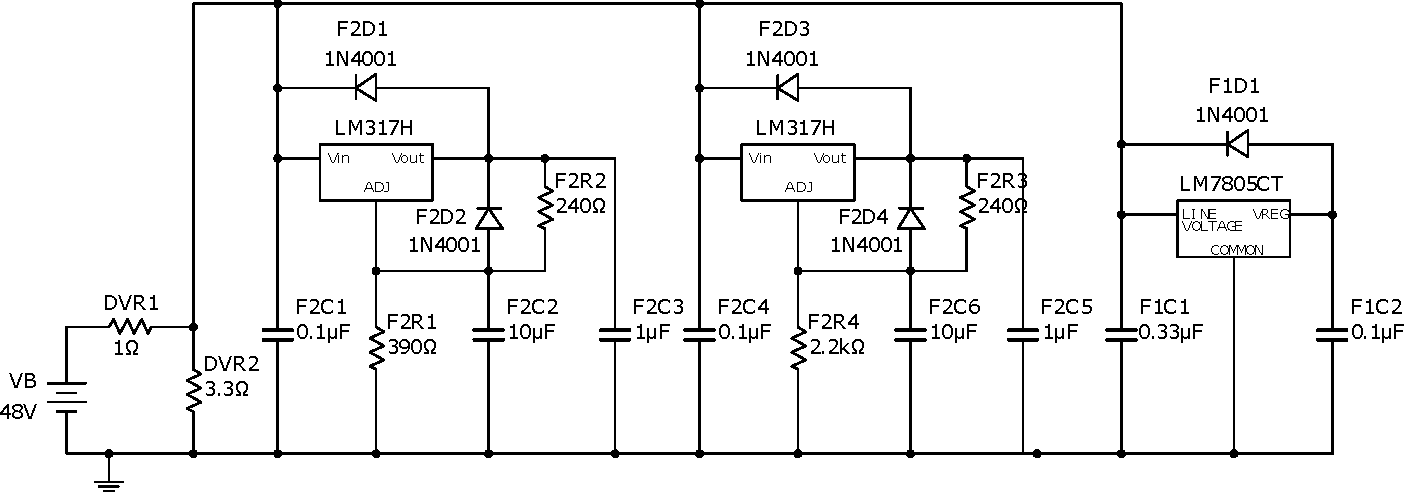
\includegraphics[width=15cm]{imagenes/fuentes3f.pdf}
	\caption{Circuito de alimentación para los componentes de CD.}
	\label{fig:vcircuitofuente}
\end{figure}

Al tener una salida del banco de baterías de 48 V, se hizo uso de un divisor de tensión obteniendo una tensión de salida de 33 V, tensión permitida por los reguladores a utilizar.\\

Para la alimentación de los motores, es necesaria una fuente de 90 V en corriente directa. Al tener un sistema con tensión nominal de 48 V, es imposible solo conectar los motores a ella y que estos funcionen. Es por eso que se optó por hacer uso de un convertidor de potencia dc / dc tipo boost, el cual permite, a través de un inductor y un capacitor, almacenar energía para elevar la corriente que proviene de la fuente de alimentación y después usarla para inyectar al capacitor y de esta manera producir niveles de tensión mayores a la salida que los de entrada. 

Se seleccionó el módulo de aumentar voltaje convertidor de voltaje elevador de la marca Walfront, el cual se alimenta con una tensión de entrada de 10 a 60 V, arrojando a la salida tensiones entre los 12 y 90V, soportando una corriente  máxima de salida de 20A.

En la figura \ref{fig:diagramaSFA} se muestra el diagrama del sistema fotovoltaico autónomo, con las características del mismo y las fuentes para alimentar los componentes de CD.

\newpage
\begin{figure}[H]
\centering
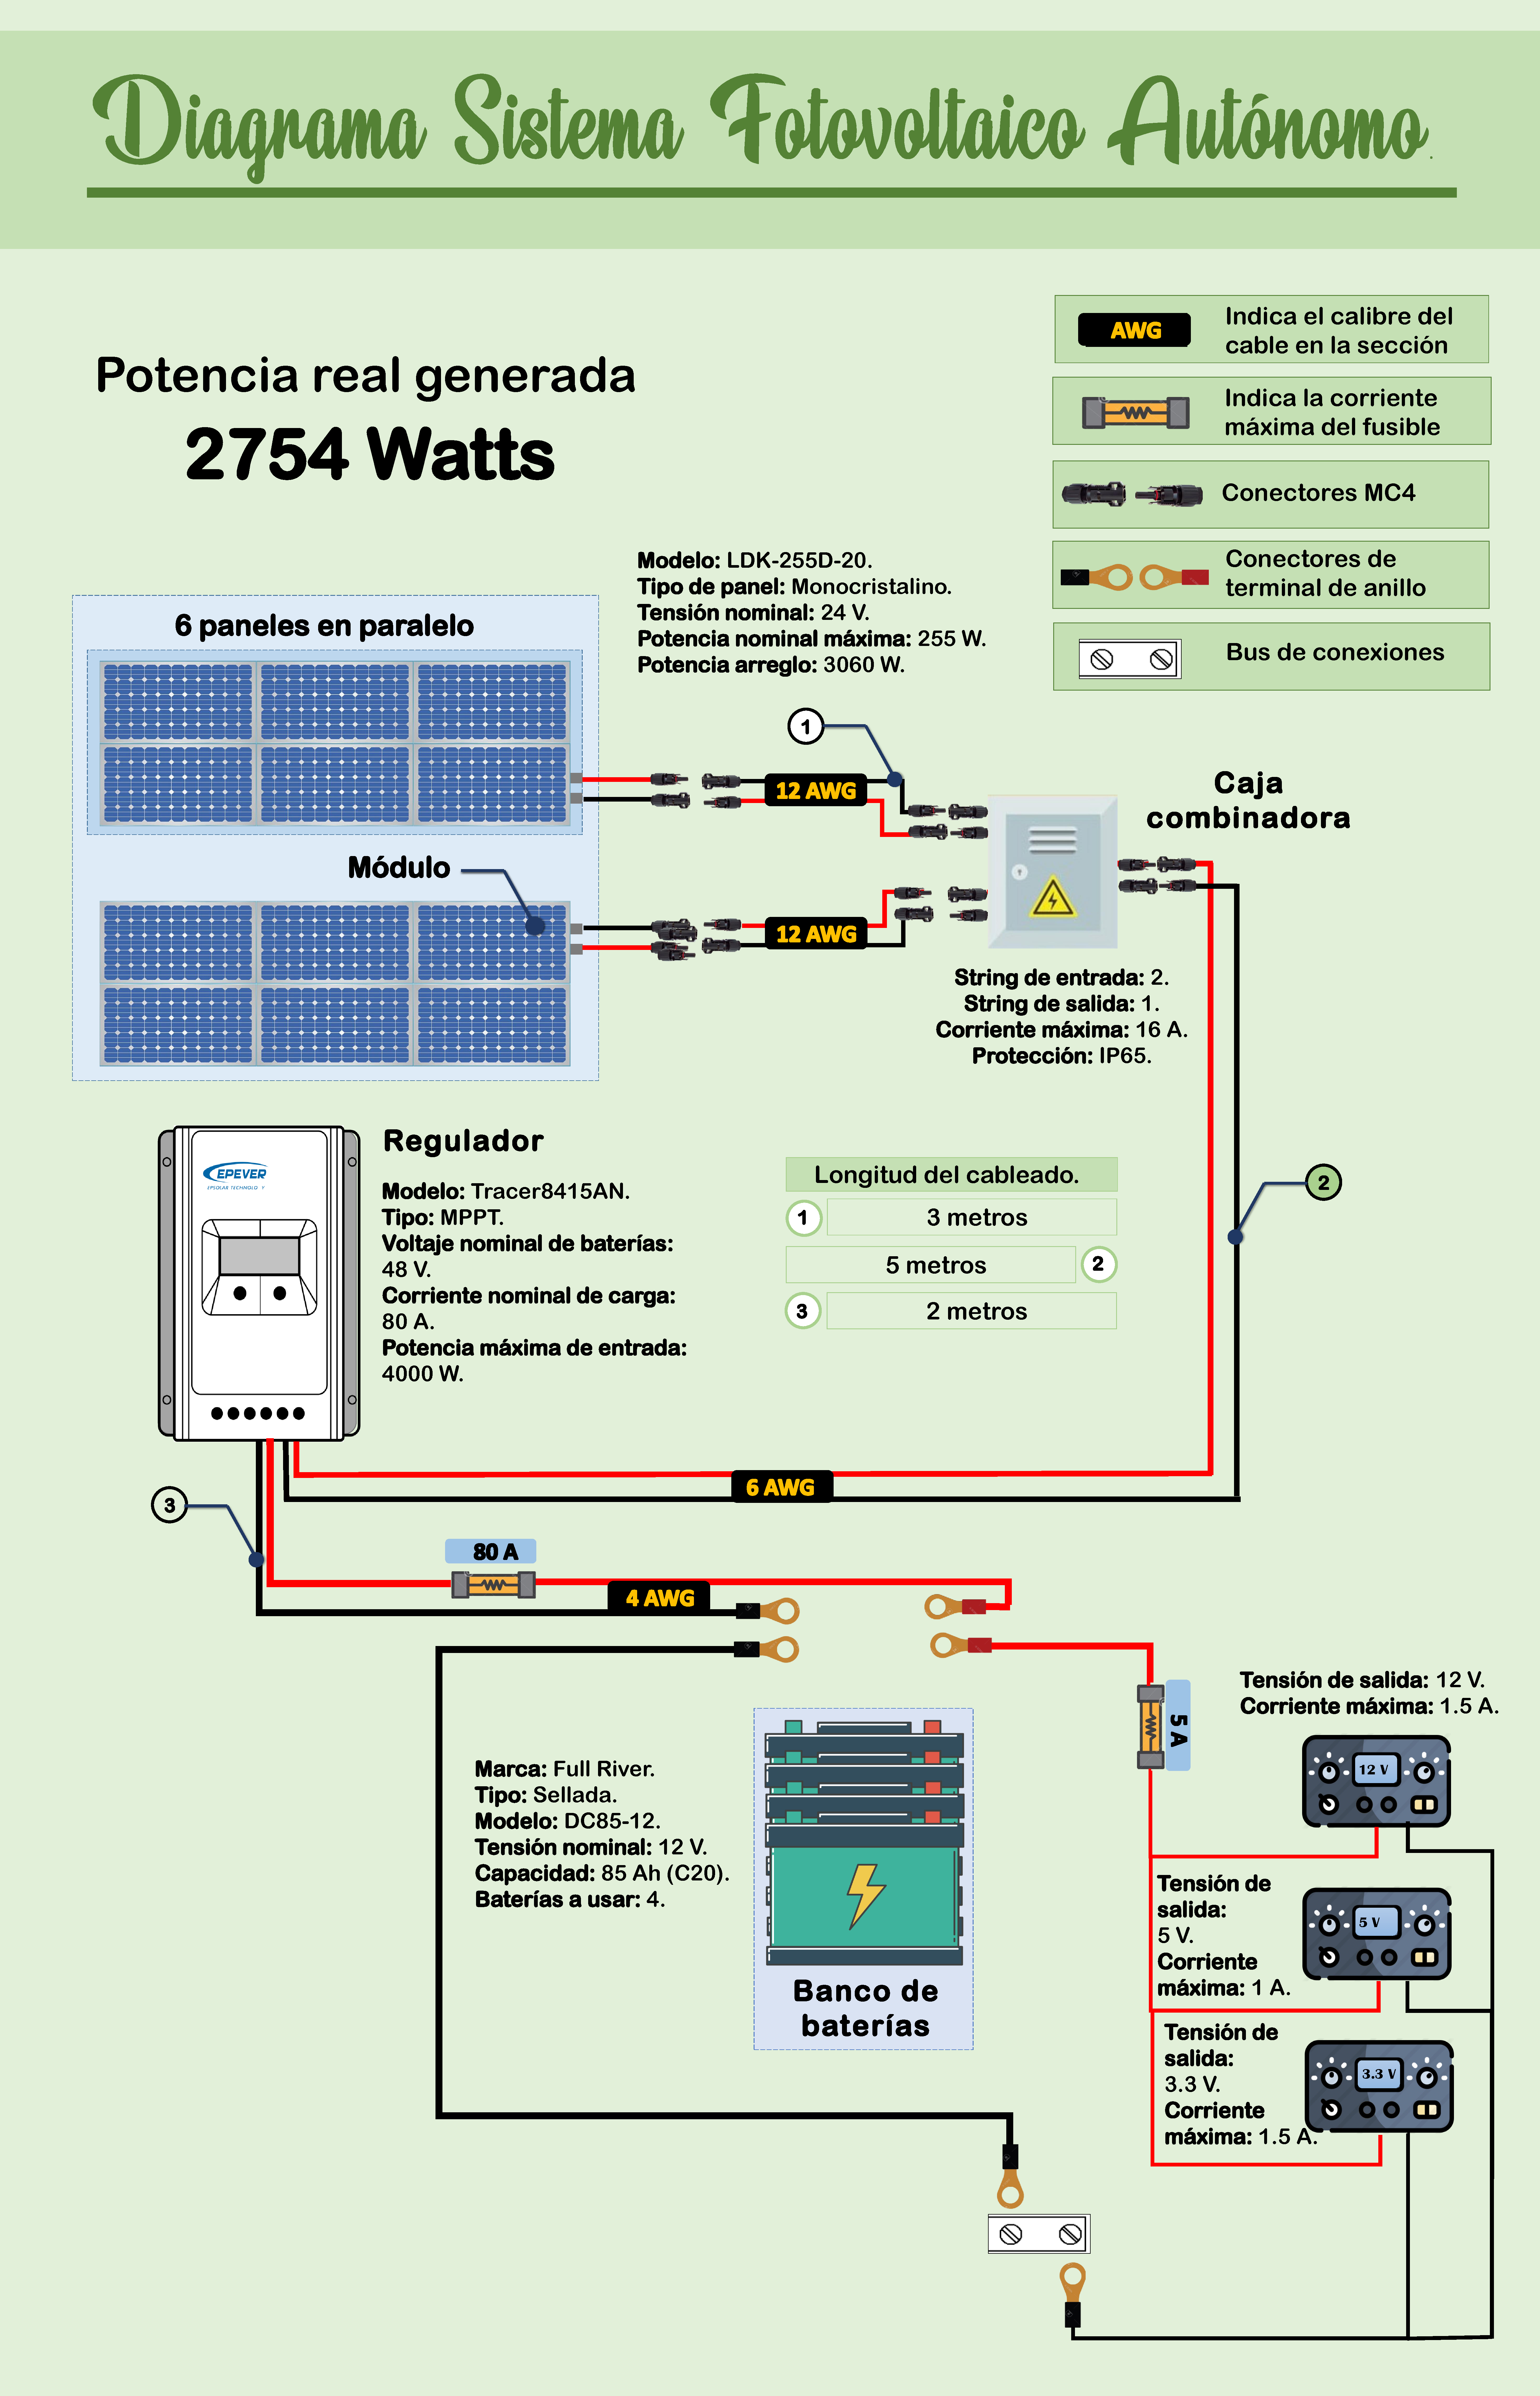
\includegraphics[width=13.5cm]{imagenes/dia_sininversor.pdf}
\caption{Diagrama SFA.}
\label{fig:diagramaSFA}
\end{figure}

\subsubsection{Validación (Sistema Energético)}
Para validar el sistema energético se hizo uso de 4 herramientas, una para validar los cálculos realizados en la selección del regulador, otra para validar el medio de almacenamiento y la última para validar la sección del cableado.

A continuación, se explica cada validación realizada:

\begin{itemize}
	\item \textbf{Regulador.}
	Para esta validación se utilizó la herramienta en linea proporcionada por $ Mon Solar $, llamada CALCULADORA DE REGULADORES SOLARES, la cual calcula los valores de corriente y tensión mínimos que el regulador de carga debe soportar \cite{DDE9}. 
	\begin{enumerate}
		\item \textbf{\textit{Selección tipo de regulador}}. Permite centrar la búsqueda a un solo tipo de regulador que sea capaz de cubrir con los parámetros del sistema.
		\item \textbf{\textit{Selección tipo de panel solar}}. Se agregan las características de los paneles a utilizar (tensión y corriente) y el número de paneles conectados, tanto en serie como en paralelo.
		\item \textbf{\textit{Selección tensión batería}}. Se selecciona el valor de la tensión nominal del sistema, mostrando una advertencia en caso de no ser la más adecuada o no cubrir las tensiones y corrientes requeridas por el sistema. 
			
		Una vez ingresados estos valores, el programa muestra los valores de tensión y corriente que habrá entre los paneles conectados en serie y en paralelo, así como los valores mínimos de corriente y tensión que el regulador debe soportar. En la Figura \ref{fig:reguladorsel} se pueden observar los valores mínimos necesarios del regulador de carga a seleccionar. Como se puede notar, el regulador de carga ganador cumple con los requerimientos mínimos. 
		
		\begin{figure}[H]
		\centering
		\includegraphics[width=8cm]{imagenes/reguladorsel}
		\caption{Calculadora de reguladores solares, MON SOLAR \cite{DDE9}.}
		\label{fig:reguladorsel}
		\end{figure}
		
	\end{enumerate}
	
	\item \textbf{Sección cableado.}
	La herramienta utilizada para la validación pertenece a $ Mon Solar $, y se llama CALCULADORA SECCIONES CABLES ELÉCTRICOS. Ésta herramienta se encarga de calcular la sección del cableado que habrá entre los componentes \cite{DDE10}. 
	
	Divide el sistema en tramos, de manera que se calcula la sección de cable entre cada componente. Se deben de introducir los valores de la longitud entre los componentes, así como la corriente y tensión que pasan por ellos. También se debe seleccionar un porcentaje de pérdidas para cada tramo. Ingresando esos valores el programa se encarga de calcular la sección del cable a utilizar, así como un porcentaje de perdidas de tensión.
	
	Ingresando los mismos valores utilizados para los cálculos realizados, se puede observar en la Figura \ref{fig:cableadoval} que, tanto los valores de sección calculados por medio de las ecuaciones como los proporcionados por la herramienta coinciden.
		
	\begin{figure}[H]
		\centering
		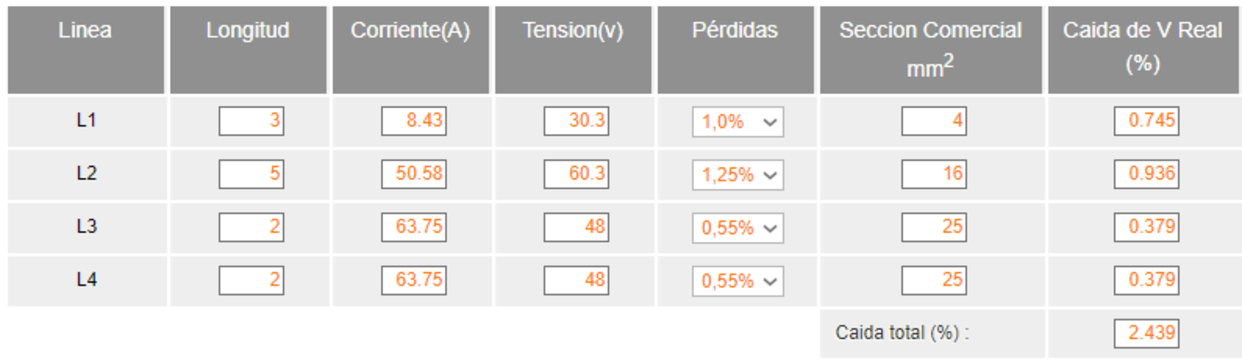
\includegraphics[width=12cm]{imagenes/cableadoval}
		\caption{Calculadora secciones cables eléctricos, MON SOLAR \cite{DDE10}.}
		\label{fig:cableadoval}
	\end{figure}
	
	\item \textbf{Medio de almacenamiento.}
	La validación del medio de almacenamiento se realizó con la herramienta en línea PHOTOVOLTAIC GEOGRAPHICAL INFORMATION SYSTEM (PVGIS), de $ European Commission $, la cual permite simular sistemas fotovoltaicos conectados a la red, autónomos y seguidores fotovoltaicos \cite{DDE11}.
	
	Primero, se debe seleccionar el tipo de sistema a simular, siendo, en este caso, Grid-off. Posteriormente, se debe ingresar la siguiente información:
	
	\begin{enumerate}
		\item \textbf{\textit{Selección ubicación.}} Se debe especificar la ubicación donde se encuetra o se encontrará el sistema fotovoltaico, para determinar la irradiancia solar. 
		\item \textbf{\textit{Potencia pico instalación fotovoltaica.}} Representa la potencia total del arreglo de paneles.
		\item \textbf{\textit{Capacidad de las baterías.}} Es la capacidad total del arreglo de baterías.
		\item \textbf{\textit{Límite de descarga.}} Es la profundidad de descarga de las baterías.
		\item \textbf{\textit{Consumo diario.}} Es la cantidad de energía necesaria para alimentar los componentes con los que se cuenta.
		\item \textbf{\textit{Inclinación.}} Es el ángulo de inclinación respecto a la horizontal. 
		\item \textbf{\textit{Azimutal.}}  Es la orientación del arreglo fotovoltaico con respecto al Sur, -90° corresponde al Este y 90° al Oeste.
		
		Para el ángulo de elevación, se definió un valor de 19° [referencia],  mientras que el ángulo Azimutal se estableció en 0°, debido a que el sistema fotovoltaico debe estar orientado al Sur verdadero \cite{DDE8}.
		Los parámetros ingresados para la simulación se muestran en la tabla \ref{tab:parametrosPVGIS}:
		\begin{table}[H]
			\centering
			\caption{Parámetros a ingresar en la herramienta en línea PHOTOVOLTAIC GEOGRAPHICAL INFORMATION SYSTEM (PVGIS).}
			\begin{tabular}{|c|c|}
				\hline
				\textbf{Latitud} & 19.512° \\
				\hline
				\textbf{Longitud} & -99.125° \\
				\hline
				\multicolumn{1}{|p{12.145em}|}{\textbf{Potencia pico instalación fotovoltaica}} & 3060 kW \\
				\hline
				\textbf{Capacidad de las baterías} & 4080 Ah \\
				\hline
				\textbf{Límite de descarga} & 60\% \\
				\hline
				\textbf{Consumo diario} & 567.6 Wh \\
				\hline
				\textbf{Inclinación} & 19° \\
				\hline
				\textbf{Azimutal} & 0° \\
				\hline
			\end{tabular}%
			\label{tab:parametrosPVGIS}%
		\end{table}%
	\end{enumerate}
	
	Con estos valores, se obtuvieron las gráficas mostradas en las Figuras \ref{fig:batgraf1} y \ref{fig:batgraf2}.
	
	
	La gráfica de la Figura \ref{fig:batgraf1} muestra la cantidad de energía generada almacenada y no almacenada. La energía no almacenada representa una gran cantidad. Sin embargo, en el sistema solamente se almacenará el \textbf{3 \%} de la energía captada. 
	
	\begin{figure}[H]
		\centering
		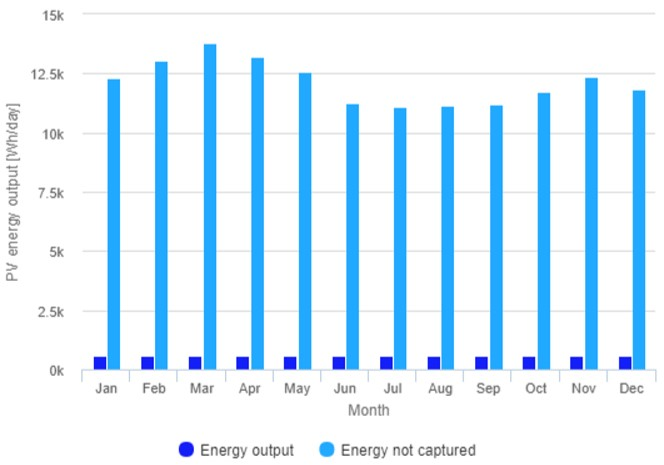
\includegraphics[width=9cm]{imagenes/batgraf}
		\caption{Producción de energía para el sistema fotovoltaico autónomo \cite{DDE3}.}
		\label{fig:batgraf1}
	\end{figure}

	En la Figura \ref{fig:batgraf2}, se muestra la gráfica del rendimiento de la batería, pudiendo notar que a lo largo del año la batería se encontrará a su máxima capacidad, siendo capaz de suministrar la energía necesaria al seguidor cuando lo requiera.

	\begin{figure}[H]
		\centering
		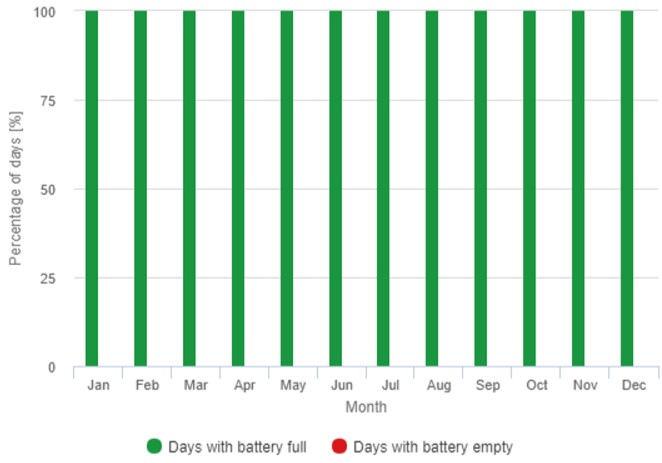
\includegraphics[width=9cm]{imagenes/batgraf2}
		\caption{Rendimiento de la batería para el sistema fotovoltaico autónomo \cite{DDE3}.}
		\label{fig:batgraf2}
	\end{figure}
	
	
	\item \textbf{Circuito alimentación en corriente directa.}
	Para validar el circuito de la Figura \ref{fig:vcircuitofuente} se realizó una simulación mediante el programa Multisim, mostrando los valores obtenidos a la salida en la Figura \ref{fig:simulacionfuentes}.

\begin{figure}[H]
	\centering
	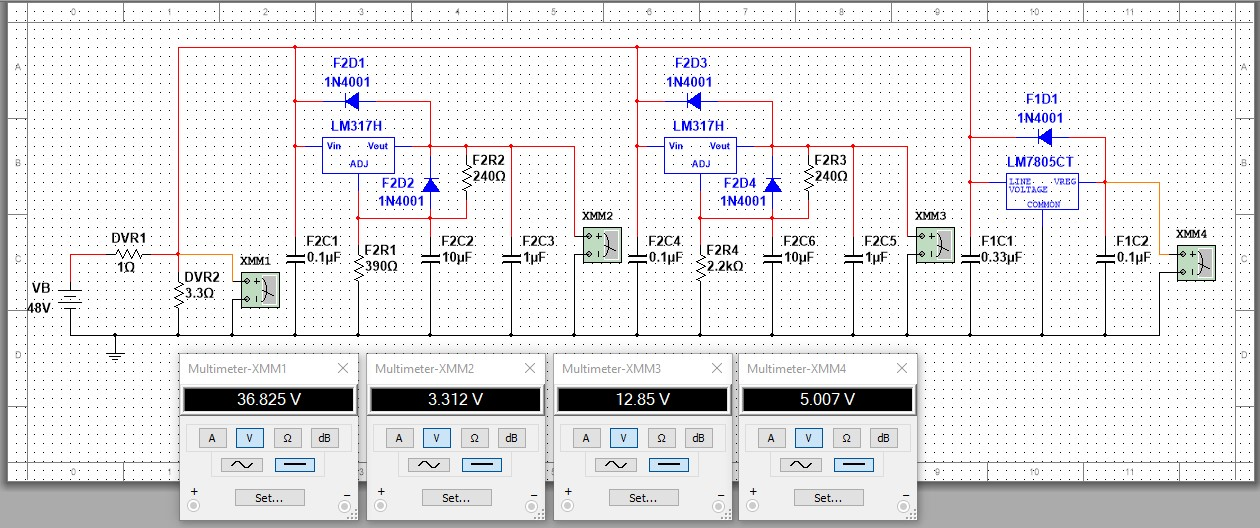
\includegraphics[width=15cm]{imagenes/Fuentes_3.jpg}
	\caption{Simulación fuentes de alimentación en el programa Multisim.}
	\label{fig:simulacionfuentes}
\end{figure}
Como se puede observar en la Figura \ref{fig:simulacionfuentes}, las salidas del divisor de tensión y de las fuentes son las necesarias para poder alimentar los componentes de CD requeridos para el seguidor.\\

\end{itemize}



\newpage
\subsection{Módulo 2: Seguimiento Solar}

En el diseño preliminar se establecieron los módulos azimutal y elevación de forma separada, ya que son relativamente independientes uno del otro. A pesar de ello, se decidió agruparlos en un solo módulo debido a que no es posible generar el modelado del robot seguidor solar para cada movimiento, ya que el robot debe analizarse en conjunto para luego determinar la mejor estrategia de control a utilizar. Además, el control tendría que describirse en ambos módulos, resultando algo redundante.

Cabe mencionar que la selección de componentes, diseño preliminar y en general el funcionamiento del seguidor, no se ven afectados por esta acción de agrupar los módulos, ya que no se alteraron las funciones, ni se crearon nuevos requerimientos ni se perdió modularidad, únicamente es para fines de claridad y simplicidad.

\subsubsection{Movimiento Azimutal}

\textbf{Elemento electromecánico de potencia}\\
Algunas de las características técnicas más relevantes del motor \textbf{MTPM-P50-1L18} se muestran en la Tabla \ref{tab:motorZ}.

\begin{table}[H]
	\centering
	\caption{Características técnicas del motor MTPM-P50-1L18 \cite{DDA1}}
	\begin{tabular}{|l|p{12.93em}|}
		\hline
		\textbf{Marca} & \multicolumn{1}{c|}{IronHorse} \\
		\hline
		\textbf{Tipo de voltaje} & \multicolumn{1}{c|}{DC} \\
		\hline
		\textbf{Tipo de motor} & \multicolumn{1}{c|}{Imanes permanentes} \\
		\hline
		\textbf{Aplicación del motor} & \multicolumn{1}{c|}{SCR-PWM} \\
		\hline
		\textbf{Potencia nominal} & \multicolumn{1}{c|}{1/2 hp} \\
		\hline
		\textbf{Voltaje nominal} & \multicolumn{1}{c|}{90 VDC} \\
		\hline
		\textbf{Velocidad síncrona} & \multicolumn{1}{c|}{1800 RPM} \\
		\hline
		\textbf{Tipo de caja} & \multicolumn{1}{c|}{TENV} \\
		\hline
		\textbf{Diámetro del eje} & \multicolumn{1}{c|}{5/8 in} \\
		\hline
		\textbf{Material de la caja} & \multicolumn{1}{c|}{Acero rolado} \\
		\hline
		\textbf{Eléctricamente reversible} & \multicolumn{1}{c|}{Sí} \\
		\hline
		\textbf{Estándar IP} & \multicolumn{1}{c|}{IP40} \\
		\hline
		\textbf{Par constante nominal} & \multicolumn{1}{c|}{20:1} \\
		\hline
	\end{tabular}%
	\label{tab:motorZ}%
\end{table}%

\newpage
\textbf{Caja reductora}

Algunas de las características técnicas más relevantes de la caja reductora \textbf{WGA-63M-100-H1} se muestran en la Tabla \ref{tab:caja_red}. Dicha caja reductora hace juego con el motor especificado anteriormente.
\begin{table}[H]
	\centering
	\caption{Características técnicas de la caja reductora WGA-63M-100-H1 \cite{DDA2}}
	\begin{tabular}{|l|p{12.93em}|}
		\hline
		\textbf{Marca} & \multicolumn{1}{c|}{IronHorse} \\
		\hline
		\textbf{Tipo de caja reductora} & \multicolumn{1}{c|}{Gusano} \\
		\hline
		\textbf{Relación de transmisión} & \multicolumn{1}{c|}{100:1} \\
		\hline
		\textbf{Rango de velocidad} & \multicolumn{1}{c|}{Entrada de 1750 RPM / salida de 18 RPM} \\
		\hline
		\textbf{Potencia nominal de entrada} & \multicolumn{1}{c|}{1/2 hp} \\
		\hline
		\textbf{Diámetro del eje de salida} & \multicolumn{1}{c|}{1.125 in} \\
		\hline
		\textbf{Par de salida mecánica} & \multicolumn{1}{c|}{1035 lb*in} \\
		\hline
		\textbf{Eficiencia mecánica ($ \nu_T $)} & \multicolumn{1}{c|}{$ 48\% $} \\
		\hline
		\textbf{Material de la carcasa} & \multicolumn{1}{c|}{Aluminio moldeado} \\
		\hline
	\end{tabular}%
	\label{tab:caja_red}%
\end{table}%
\textbf{Transmisión mecánica del movimiento azimutal}

Observando la disponibilidad de espacio dentro del tubo del soporte principal (diámetro máximo de 7.5 in) se optó por basar este diseño con un paso diametral de 12. Utilizando un programa elaborado en Mathematica para obtener la velocidad angular máxima de movimiento en función de una trayectoria gobernada por un polinomio de interpolación cúbico, se encontró que la velocidad máxima a la que se moverá este módulo será $ \omega_{out} = 0.08\ rad/s = 0.764\ RPM $, con lo que la relación de velocidades entre ésta y la velocidad de salida máxima de la caja reductora es:
\begin{equation}
	RV = \frac{\omega_{in}}{\omega_{out}} = \frac{18\ RPM}{0.764\ RPM} = 23.56
\end{equation}
Tomando un factor de seguridad de 2, se considera esta relación de velocidades como 48, con el fin de no demandar la carga máxima del motor. Con base en el procedimiento de diseño de transmisiones mecánicas desarrollado en \cite{DDA3} (páginas 341 a 347) y eligiendo el ángulo de contacto entre dientes de 20°, se obtienen las dimensiones de esta transmisión mostradas en la Tabla \ref{tab:transZ}.

\begin{table}[H]
	\centering
	\caption{Dimensiones de la transmisión del Movimiento Azimutal}
	\begin{tabular}{|l|c|c|}
		\hline
		\textbf{Parámetro} & \multicolumn{1}{l|}{\textbf{Ecuación}} & \multicolumn{1}{l|}{\textbf{Cantidad}} \\
		\hline \hline
		Roscas en el sinfín & $ N_w $ & 1 \\
		\hline
		Dientes de la corona & $ N_G = N_w * RV $ & 48 \\
		\hline
		Diámetro del sinfín & $ D_w $ & 1.5 in \\
		\hline
		Diámetro de la corona & $ D_G $ & 4 in \\
		\hline
		Paso circular & $ p = \frac{\pi}{P_d} $ & 0.262 in \\
		\hline
		Avance & $ L = N_w * p $ & 0.262 in \\
		\hline
		Ángulo de avance & $\lambda = arctan( \frac{L}{\pi * D_w} ) $ & 3.18° \\
		\hline
		Ángulo de presión & $ \phi = arctan(tan(20^o)*cos(\lambda)) $ & 19.972° \\
		\hline
		Addendum & $ a = 1/P_d $ & 0.083 in \\
		\hline
		Profundidad total & $ h_t = 2.157/P_d $ & 0.18 in \\
		\hline
		Dedendum & $ b = h_t - a $ & 0.096 in \\
		\hline
		Ancho de diente & $ e = 1.5875/P_d $ & 0.1323 in \\
		\hline
		Diámetro exterior & $ D_ow = D_w + 2a $ & 1.7 in \\
		\hline
		Diámetro raíz & $ Drw = D_w - 2b $ & 1.333 in \\
		\hline
	\end{tabular}%
	\label{tab:transZ}%
\end{table}%

\textbf{Eje del Tallo}

Este módulo debe moverse a una velocidad máxima $ \omega = 0.375\ RPM $ para transmitir un par $ \tau = 50\ Nm $ como máximo. Con base en esos datos y los de la Tabla \ref{tab:transZ}, se determinaron los esfuerzos en el eje del tallo, cuyos resultados se muestran en la Tabla \ref{tab:Feje}.
\begin{table}[H]
	\centering
	\caption{Esfuerzos en la corona del eje del Tallo}
	\begin{tabular}{|l|c|c|}
		\hline
		\textbf{Parámetro} & \multicolumn{1}{l|}{\textbf{Ecuación}} & \multicolumn{1}{l|}{\textbf{Cantidad}} \\
		\hline \hline
		Potencia & $ P = \tau * \omega $ & 1.9635 W \\
		\hline
		Momento torsionante & $ Mt = \frac{6300(\frac{P}{745.6})}{\omega} $ & 442.4185 lb*in \\
		\hline
		Fuerza tangencial & $ F_t = \frac{Mt}{0.5*D_G} $ & 221.21 lb \\
		\hline
		Velocidad de deslizamiento & $ v_s = \frac{\pi * D_G * \omega}{12*sin(\lambda)} $ & 0.7413 ft/min \\
		\hline
		Coeficiente de fricción & $ \mu = 0.124 * e^{-0.074*v_s^{0.645}} $ & 0.11666 \\
		\hline
		Fuerza radial & $ F_r = \frac{F_t * sin(\phi)}{cos(\phi)cos(\lambda) - \mu * sin(\lambda)} $ & 81.075 lb \\
		\hline
	\end{tabular}%
	\label{tab:Feje}%
\end{table}%

Para la carga del viento, retomando la velocidad máxima del viento calculada $ v_w = 31.5\ m/s $, se utilizó la Ecuación \ref{eq:viento}, la cual ya fue descrita en el módulo estructural.
\begin{equation} \label{eq:viento}
    F_w = 0.5*C_d*\rho*A_{ef}*v_d^2
\end{equation}
\begin{itemize}
	\item $ A_{ef} = 3*L1*4*L2 $: área máxima de ataque, en donde
	\begin{itemize}
		\item $ L1 = 1.642\ m $: longitud larga de cada panel.
		\item $ L2 = 0.994\ m $: longitud corta de cada panel.
	\end{itemize}
\end{itemize}

El resto de las variables se especificaron en la Tabla \ref{tab:carga_colector}, de donde se obtiene la carga del viento $ F_w = 23710\ N $, que en libras es $ F_w = 5330\ lb $, la cual corresponderá a la carga $ P_2 $. Con este dato, se elaboró el diagrama de cuerpo libre de la Figura \ref{fig:tallo1} en el software MDSolids (la posición exacta de $P_1$ es $x=6.25\ in$, pero el software redondeó su valor).

\begin{figure}[H]
	\centering
	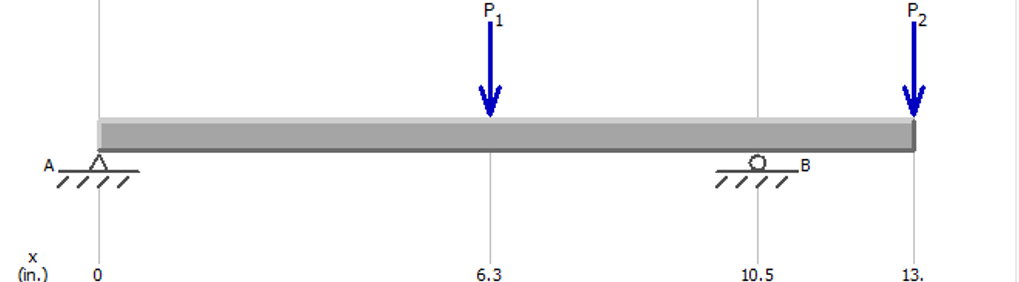
\includegraphics[width=\columnwidth]{imagenes/talloDCL}
	\caption{Diagrama de cuerpo libre del eje del tallo}
	\label{fig:tallo1}
\end{figure}

Con base en los resultados de la simulación se obtuvieron las reacciones y momentos presentes en el eje, mostrados en la Tabla \ref{tab:tallo1}.
\begin{table}[H]
	\centering
	\caption{Resultados de la simulación}
	\begin{tabular}{|l|l|l|}
		\hline
		\textbf{Carga $ P_1 $} & \textbf{Reacciones (lb)} & \textbf{Momentos (lb*in)} \\
		\hline \hline
		\multirow{2}[4]{*}{$ F_t $} & $ R_{At}=-1179.51 $ & $ M_{At}=7371.94 $ \\
		\cline{2-3}          & $ R_{Bt}=6730.72 $ & $ M_{Bt}=13325 $ \\
		\hline
		\multirow{2}[4]{*}{$ F_r $} & $ R_{Ar}=-1236.23 $ & $ M_{Ar}=7726.45 $ \\
		\cline{2-3}          & $ R_{Br}=6647.31 $ & $ M_{Br}=13325 $ \\
		\hline
	\end{tabular}%
	\label{tab:tallo1}%
\end{table}%

Los momentos flexionantes de cada apoyo son los siguientes:
\begin{equation}
M_A = \sqrt{M_{At}^2 + M_{Ar}^2} = 10679.1165\ lb*in
\end{equation}
\begin{equation}
M_B = \sqrt{M_{Bt}^2 + M_{Br}^2} = 18844.4\ lb*in
\end{equation}

Con base en \cite{DDA3} se obtiene el diámetro crítico, eligiendo los coeficiente $ kf\ y\ kt $ de la Tabla \ref{tab:coef} con valores de 2 y 1.5 respectivamente, considerando movimiento en lapsos cortos.
\begin{table}[H]
	\centering
	\caption{Coeficiente kf y kt}
	\begin{tabular}{|l|c|c|}
		\hline
		\textbf{Condición de carga} & \multicolumn{1}{l|}{\textbf{kf}} & \multicolumn{1}{l|}{\textbf{kt}} \\
		\hline \hline
		Carga aplicada gradualmente & 1.5   & 1.0 \\
		\hline
		Carga repetitiva (choque menor) & 1.5 a 2.0 & 1.0 a 1.5 \\
		\hline
		Carga repetitiva (choque mayor) & 2.0 a 3.0 & 1.5 a 3.0 \\
		\hline
	\end{tabular}%
	\label{tab:coef}%
\end{table}%

Al considerar como material \textbf{Aluminio 6063 T6}, el $ \sigma_{perm} = 40000\ psi $. Tomando a $M_B$ como el momento flexionante máximo, el diámetro mínimo del eje del Tallo será:

\begin{equation}
d=\sqrt[3]{\frac{16}{\pi*\sigma_{perm}}*\sqrt{(kf*M_{max})^2+(kt*Mt)^2}}=1.6868\ in
\end{equation}

Así, se propone que el diámetro del eje del Tallo sea de \textbf{2\ in}.\\

\textbf{Chavetas de los ejes de movimiento azimutal}

Con base en la Tabla expuesta en \cite{DDA3} (página 495), se seleccionó una chaveta de perfil cuadrangular, ya que el diámetro del eje no excede las $ 6 \frac{1}{2}\ in $. Dado que el eje del Tallo será de 2 in, la chaveta tendrá un ancho de $ \frac{1}{2}\ in$. El material de la chaveta será de acero al bajo carbón, con estirado en frío \textbf{AISI 1020}, con resistencia a la fluencia de \textbf{350 MPa}.

Tomando en cuenta el par al que estará sometido el eje del Tallo ($ \tau =50\ Nm= 442.5373\ lb*in$), se tiene que la longitud mínima de la chaveta debe ser de:
\begin{eqnarray}
L_m=\frac{4\tau}{\sigma_{p}DH}=0.035\ in
\end{eqnarray}
El largo de la chaveta igual al grosor de la corona de azimutal, es decir, de \textbf{1.75\ in}.\\

\textbf{Anillo de retención para el eje del Tallo}

Considerando que el eje del Tallo será de 2 in, se seleccionó en \cite{DDA4} el anillo de retención $ SH-200 $, el cual es un anillo de eje para ensamble externo. Este tendrá la función de sostener la corona de Azimutal para evitar su desplazamiento axial en el eje.\\

\textbf{Rodamientos y chumaceras de los ejes de movimiento azimutal}

La selección de rodamientos se realizó con base en \cite{DDA5}. Para ello, se requiere conocer la carga resultante que tendrá cada uno de estos. De los resultados de la Tabla \ref{tab:tallo1}, se calcularon las cargas máximas que tendrá que soportar cada rodamiento.
\begin{equation}
R_A=\sqrt{R_{At}^2+R_{Ar}^2}=1710\ lb \approx 7.6\ kN
\end{equation}
\begin{equation}
R_B=\sqrt{R_{Bt}^2+R_{Br}^2}=9460\ lb \approx 42.1\ kN
\end{equation}
El rodamiento para soportar $ R_A $ será el $ HR 32909 J $, el cual resiste una carga máxima de $ 34.5\ kN $, mientras que el rodamiento para soportar $ R_B $ será el $ HR 32912 J $, el cual resiste una carga máxima de $ 49\ kN $.

Para soportar el eje del tornillo sinfín de azimutal se seleccionó, con base en el diámetro del eje, la chumacera $ SN 507 $ con rodamiento de bolas autolineantes $ 1207 K $, el cual soporta una carga máxima de $ 5.1\ kN $.

%\subsubsection{Sensores de posición}
\textbf{Encoder del motor de movimiento azimutal}

Para realizar la correcta selección del encoder se siguió el árbol de decisiones de la Figura \ref{fig:encoder1}, seleccionando la marca Koyo debido a su alta confiabilidad en cuanto a precisión. Se inicia con 261 tipos de encoders, entre ellos de trabajo ligero, mediano y pesado, así como encoders incrementales y absolutos.

\begin{figure}[H]
	\centering
	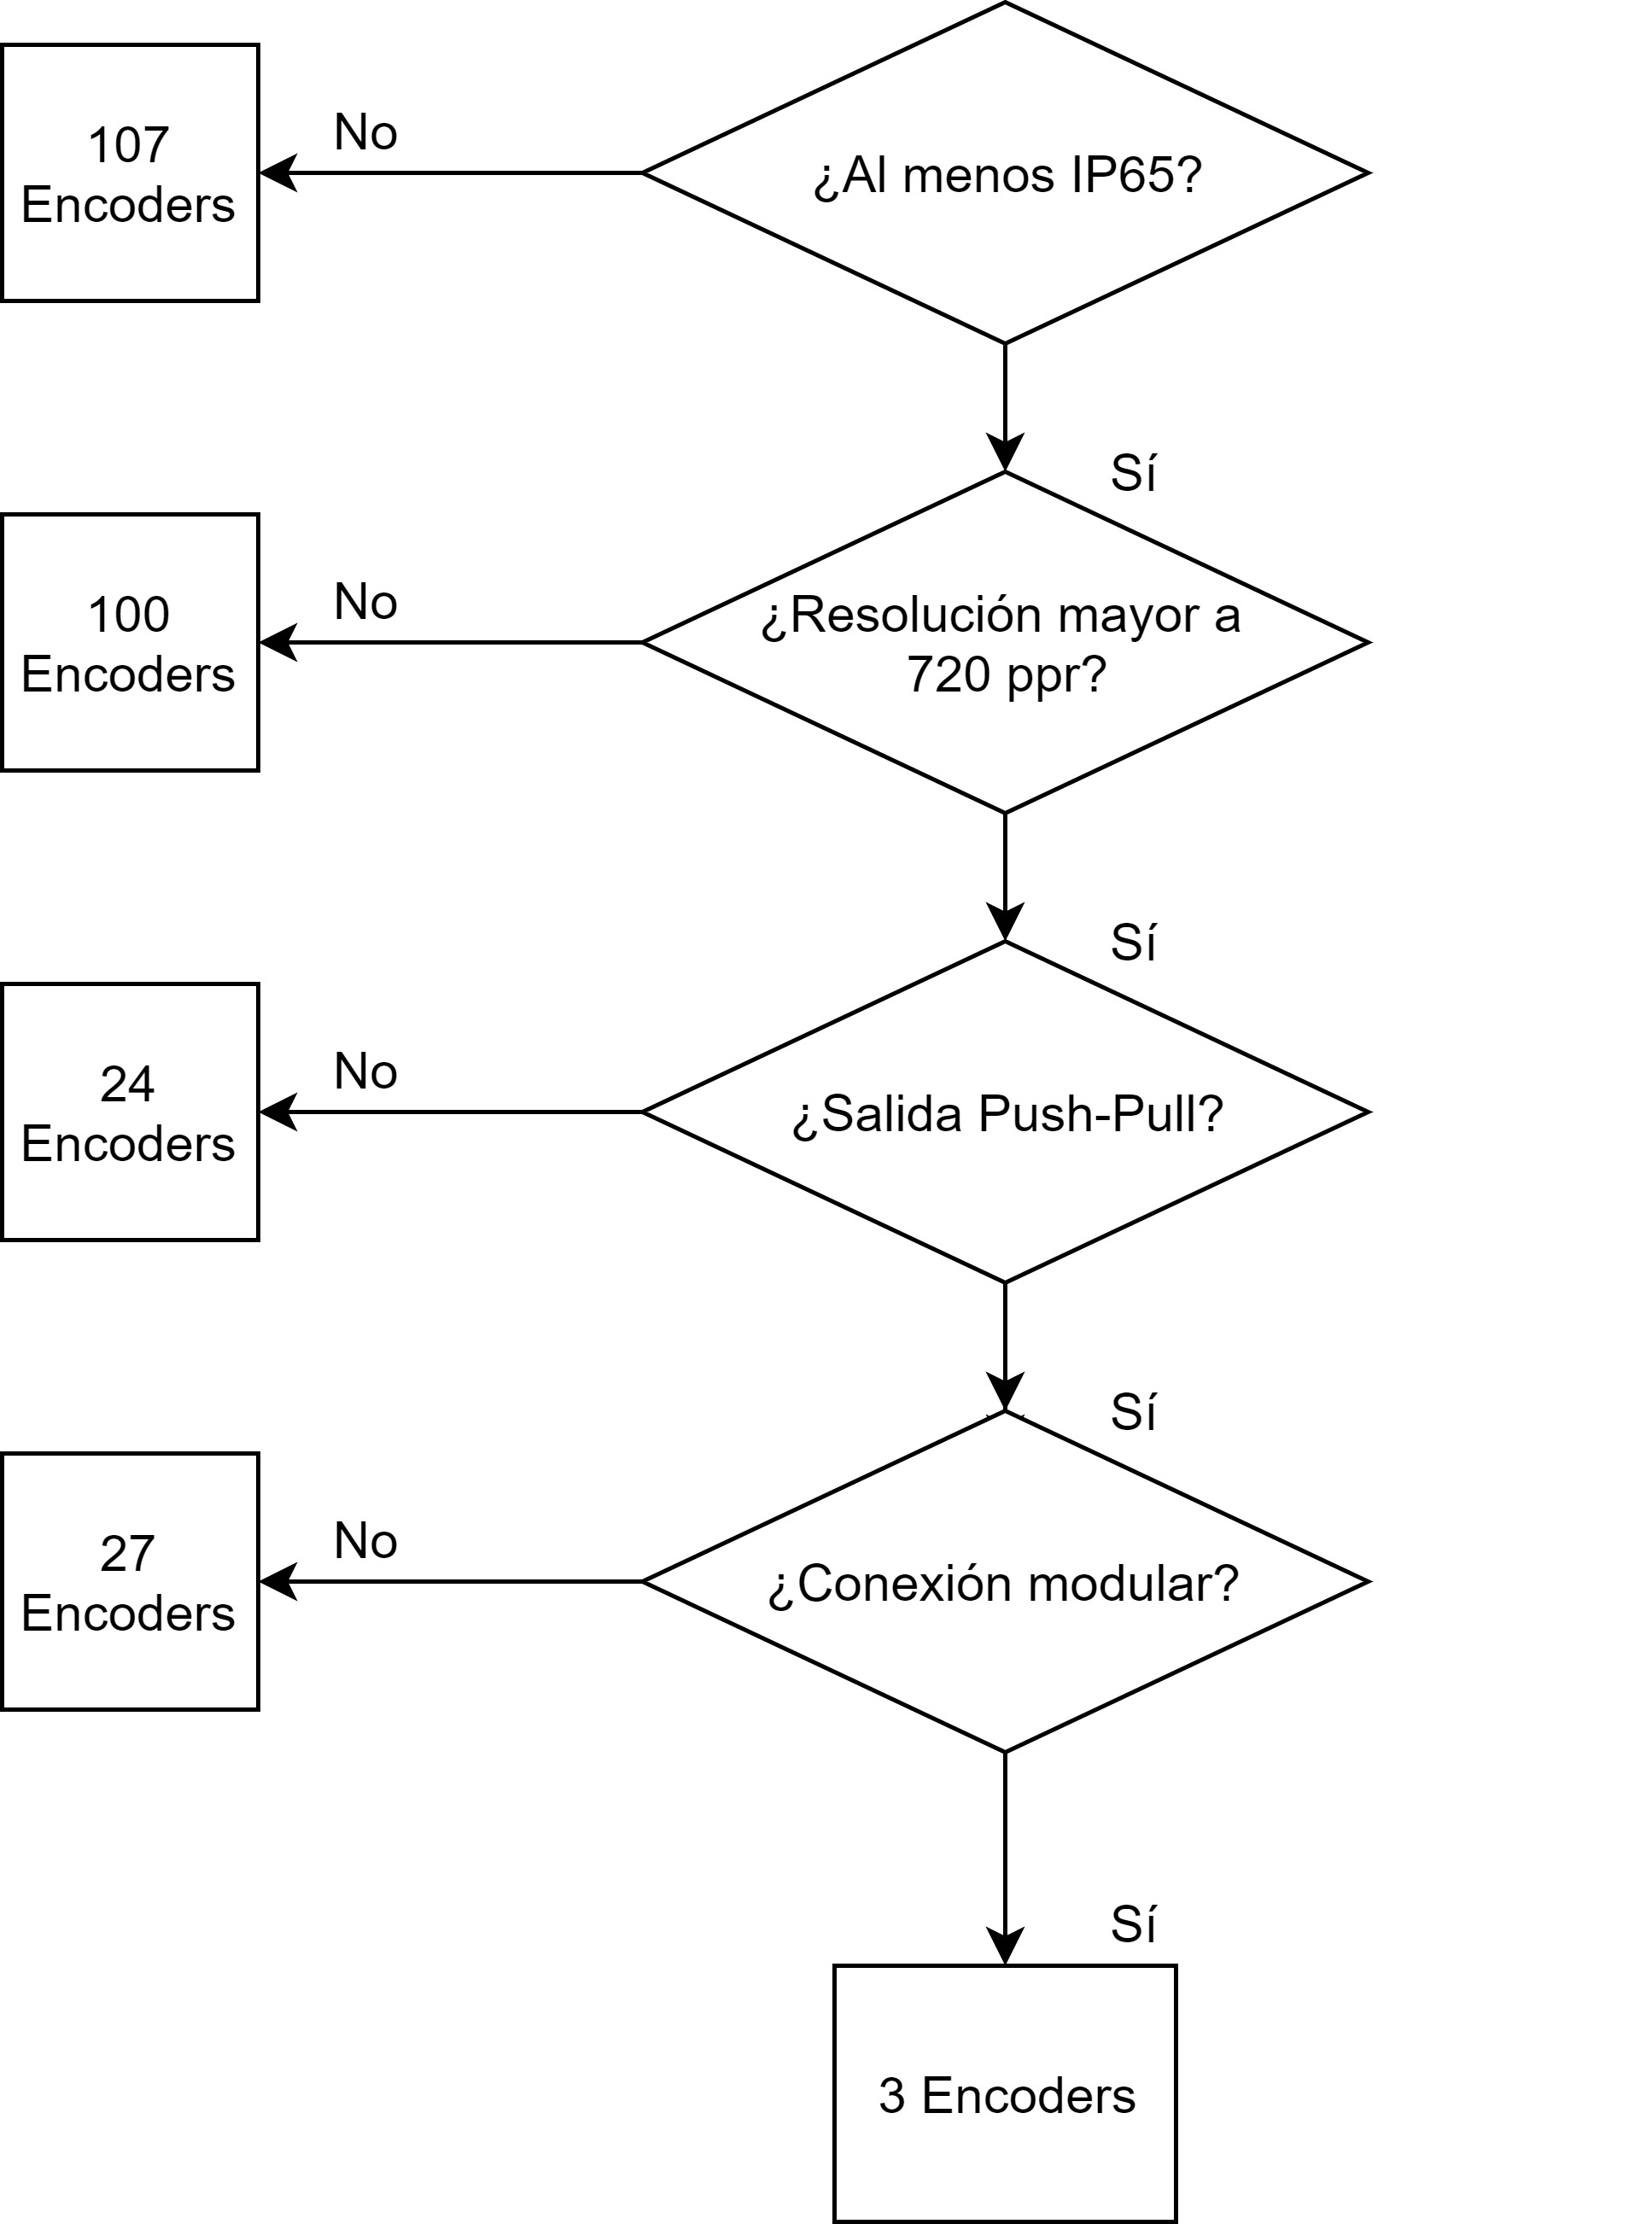
\includegraphics[width=7cm]{imagenes/encoder1}
	\caption{Árbol de decisiones para selección del encoder}
	\label{fig:encoder1}
\end{figure}

\newpage
\begin{itemize}
	\item Tipo de protección: IP65, la mayor dentro del catálogo de encoders.
	\item Incremental: Requiere menos líneas de conexión y se puede ajustar su resolución.
	\item Resolución: Al menos de 720 ppr para obtener una precisión de 0.5°.
	\item Tipo de conexión: Montaje modular, conexión denominada \textit{Conector estilo militar (MS)}, permitiendo que el encoder se pueda separar del cable de conexión.
\end{itemize}

Se seleccionó el encoder con mayor resolución y menor costo (utilizando AHP), con matrícula: \underline{\textit{TRDA25RN2500VWDMS}}. Sus características se muestran en la Tabla \ref{tabla:caracteristicas} \cite{DDA6}.\\

\textbf{\textit{Sensor de final de carrera del movimiento azimutal}}

Se consideraron los siguientes criterios para la selección de este sensor:
\begin{itemize}
	\item Grado de protección industrial: debe de ser al menos IP65.
	\item Velocidad de acción: rápida, al mínimo contacto se activa el sensor.
	\item Normalmente abierto: disminuir consumo energético cuando el sensor no esté activo.
	\item Modularidad: con cable de conexión independiente.
	\item Flexibilidad: sensor ajustable, ya que su posición se fijará al construir el módulo.
	\item Material del interruptor: metálico para disminuir la fricción entre éste y la pieza mecánica que active al sensor.
\end{itemize}

\begin{figure}[H]
	\centering
	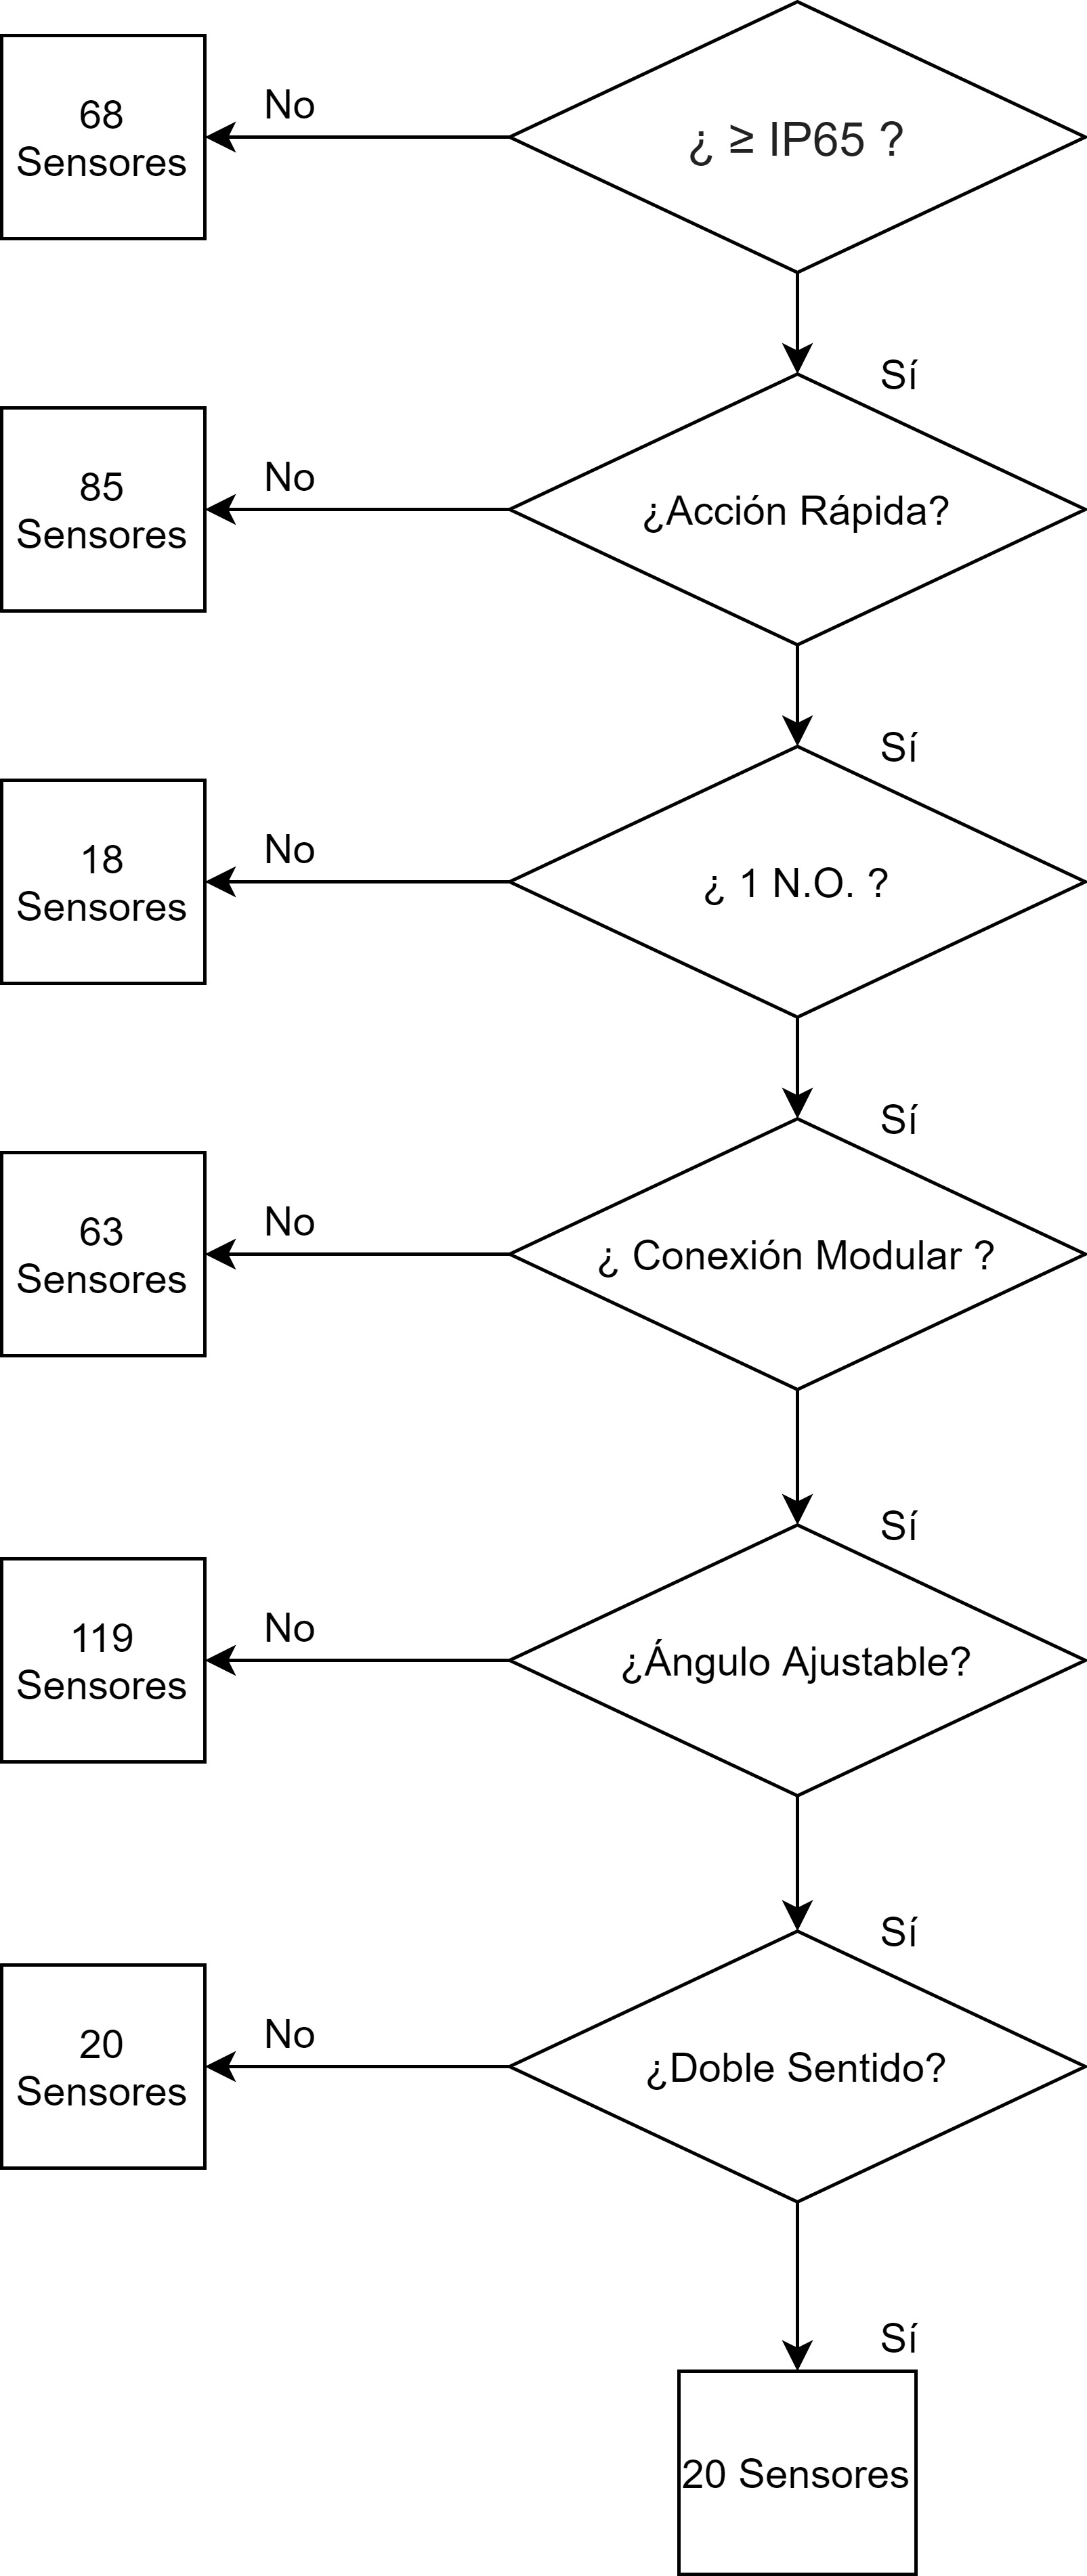
\includegraphics[width=5cm]{imagenes/limit1}
	\caption{Árbol de decisiones para la selección del sensor de final de carrera}
	\label{fig:limitZ}
\end{figure}

En este módulo se requiere que el sensor detecte desde ambos laterales, por lo que se consideraron los sensores de la familia \textit{Palanca giratoria lateral con actuador de rodillo}. Utilizando criterios de selección (precio, grado de protección industrial, tamaño, material, facilidad de montaje) y la herramienta AHP, el sensor seleccionado fue el siguiente: \underline{\textit{AEM2G4520Z11MR}}. Las características de este dispositivo se muestran en la Tabla \ref{tabla:caracteristicas} \cite{DDA7}.

\subsubsection{Movimiento de Elevación}
En este módulo se considera un motor de corriente directa con las mismas especificaciones de la Tabla \ref{tab:motorZ}. Así mismo, se emplea la misma caja reductora del Módulo de Movimiento Azimutal con las especificaciones de la Tabla \ref{tab:transZ}.

\textbf{Transmisión mecánica del movimiento de elevación}\\

Para mover el colector, se considera que este tiene una masa de media tonelada, así que su peso resulta ser $ W_C=5\ kN $. El brazo de palanca máximo entre el colector y su eje es de \textbf{30 cm}, por lo que el momento flector máximo que deberá de soportar el eje del Colector será $ Mt=1500\ N*m $.\\

Los materiales de los que estarán hechos la corona y el tornillo sinfín serán de bronce y acero respectivamente. Se propone entonces un coeficiente de fricción $ \mu=0.15 $ para obtener una relación irreversible en la transmisión. \\

Proponiendo que el Colector puede moverse de 0° a 180° en 60 segundos, se utilizó un polinomio de interpolación cúbico que representa la posición angular del Colector, al derivarlo (utilizando el software Mathematica) se encontró la función de la velocidad, de la cual se obtuvo que la velocidad máxima a la que se mueve el Colector será $ \omega_{MAX}=0.03927\ rad/s=0.375\ RPM $. Tomando la velocidad de salida de la caja reductora dada en la Tabla \ref{tab:caja_red} ($ \omega_{out}=18\ RPM $), se tiene que la relación de velocidades para este modulo será de:
\begin{equation}
    RV = \frac{\omega_{out}}{\omega_{MAX}} = 48
\end{equation}
Con base en estos datos y en \cite{DDA10}, se realizaron los cálculos mostrados en la Tabla \ref{tab:modele}, cuyos resultados establecen el punto de partida del diseño de la transmisión corona-sinfín.
\begin{table}[H]
	\centering
	\caption{Cálculo del módulo para la transmisión del movimiento de Elevación}
	\begin{tabular}{|l|c|c|}
		\hline
		\textbf{Parámetro} & \multicolumn{1}{l|}{\textbf{Ecuación}} & \multicolumn{1}{l|}{\textbf{Cantidad}} \\
		\hline \hline
		Roscas en el sinfín & $ N_w $ & 1 \\
		\hline
		Dientes de la corona & $ N_G = N_w * RV $ & 48 \\
		\hline
		Potencia consumida & $ P_{cons}=\frac{M_t*\omega_{MAX}}{716200} $ & 0.08 HP \\
		\hline
		Potencia suministrada & $ P_{sum}=\frac{P_{cons}}{\eta_T} $ & 0.1668 HP \\
		\hline
		Ángulo de fricción & $ \rho=\arctan(\mu) $ & 8.53° \\
		\hline
		Factor K & $ k $ & 3.4 \\
		\hline
		Coeficiente de carga & $ c $ & 60 \\
		\hline
		Ángulo de avance  & $\beta=\arctan(\frac{N_w}{2k})$ & 8.366° \\
		\hline
	\end{tabular}%
	\label{tab:modele}%
\end{table}%

Para continuar, se analiza la fuerza normal (descompuesta en dos fuerzas: $ f1 $ y $ f2 $) entre un diente de la corona y filete del tornillo sinfín.

\begin{table}[H]
	\centering
	\caption{Relaciones de la transmisión}
	\begin{tabular}{|l|c|}
		\hline
		\textbf{Parámetro} & \multicolumn{1}{l|}{\textbf{Ecuación}} \\
		\hline \hline
		Profundidad del diente & $ h=\frac{\pi N_w m_n}{\cos(\beta)} $ \\
		\hline
		Paso circular & $ \rho_c=\frac{\pi m_n}{\cos(\beta)} $ \\
		\hline
		Ancho de la corona & $ b=7\frac{m_n}{\cos(\beta)} $ \\
		\hline
		f1 & $ \frac{60(75)P_{sum}}{h \omega_{out}} $ \\
		\hline
		f2 & $ 60bh $ \\
		\hline
		Relación entre f1 y f2 & $ f_1=f_2\tan(\beta+\rho) $ \\
		\hline
	\end{tabular}%
	\label{tab:relA}%
\end{table}%

Utilizando las expresiones de la Tabla \ref{tab:relA} se obtiene la expresión para calcular el módulo normal de esta transmisión:
\begin{equation}
	m_n=\sqrt[3]{\frac{(75)P_{sum}}{7 \pi^2 N^2_w \omega_{out} \tan(\beta+\rho)}}\cos(\beta)=3.375\ mm^{-1}
\end{equation}

Se diseña la transmisión del Módulo de Elevación tomando como base un módulo de $ 3.5\ mm^{-1} $. Con base en el procedimiento de diseño de transmisiones mecánicas desarrollado en \cite{DDA10} (páginas 77 a 80), y tomando el ángulo de contacto de los dientes de 14.5°, se obtuvieron las dimensiones de esta transmisión mostradas en la Tabla \ref{tab:transA}.

\begin{table}[H]
	\centering
	\caption{Dimensiones de la transmisión del Movimiento Azimutal}
	\begin{tabular}{|l|c|c|}
		\hline
		\textbf{Parámetro} & \multicolumn{1}{l|}{\textbf{Ecuación}} & \multicolumn{1}{l|}{\textbf{Cantidad}} \\
		\hline \hline
		Roscas en el sinfín & $ N_w $ & 1 \\
		\hline
		Dientes de la corona & $ N_G = N_w * RV $ & 48 \\
		\hline
		Diámetro del sinfín & $ D_w $ & 24.056 mm \\
		\hline
		Diámetro de la corona & $ D_G $ & 169.807 mm \\
		\hline
		Paso circular & $ p = \frac{\pi}{P_d} $ & 11.114 mm \\
		\hline
		Avance & $ L = N_w * p $ & 50.235 mm \\
		\hline
		Ángulo de avance & $\lambda = arctan( \frac{L}{\pi * D_w} ) $ & 8.366° \\
		\hline
		Ángulo de presión & $ \phi = arctan(tan(20^{o})*cos(\lambda)) $ & 14.35° \\
		\hline
		Addendum & $ a = 1/P_d $ & 3.5 mm \\
		\hline
		Profundidad total & $ h_t = 2.157/P_d $ & 7.55 mm \\
		\hline
		Dedendum & $ b = h_t - a $ & 4.05 mm \\
		\hline
		Ancho de diente & $ e = 1.5875/P_d $ & 5.55625 mm \\
		\hline
		Diámetro exterior & $ D_ow = D_w + 2a $ & 31.056 mm \\
		\hline
		Diámetro raíz & $ Drw = D_w - 2b $ & 15.956 mm \\
		\hline
	\end{tabular}%
	\label{tab:transA}%
\end{table}%

\textbf{Eje del Colector}

Por medio de la simulación hecha en la GUI de MatLab, se encontró que el ángulo en el cual se presenta el mayor momento flexionante en el Colector es $ \theta=8.05^o $. Con este dato, se obtuvieron las reacciones en la corona presentadas en la Tabla \ref{tab:fcorona}. Previamente se obtuvo el valor numérico de las reacciones debidas al contacto entre corona y tornillo $ f1 $ y $ f2 $.
\begin{equation}
	f1=\frac{60(75)P_sum}{h \omega_{out}} =4498.9\ N
\end{equation}
\begin{equation}
	f2=60bh=16513.062\ N
\end{equation}

\begin{table}[H]
	\centering
	\caption{Cálculo de las reacciones en la corona}
	\begin{tabular}{|l|c|c|}
		\hline
		\textbf{Parámetro} & \multicolumn{1}{l|}{\textbf{Ecuación}} & \multicolumn{1}{l|}{\textbf{Cantidad}} \\
		\hline \hline
		Fuerza normal & $ F_N=f1*\frac{\cos(\rho)}{\sin(\beta+\rho)}= f2*\frac{\cos(\rho)}{\cos(\beta+\rho)} $ & 17067.122 N \\
		\hline
		Fuerza radial & $ Fr=F_N \sin(\theta) $ & 4273.266 N \\
		\hline
		Fuerza axial & $ Fa=F_N (\sin\beta\cos\theta+\mu\cos\beta) $ & 4936.93 N \\
		\hline
		Fuerza tangencial & $ Ft=F_N (\cos\beta\cos\theta+\mu\sin\beta) $ & 16720.15 N \\
		\hline
		Momento axial & $ Ma=\frac{D_G Fa}{2} $ & 419.17 N*m \\
		\hline
	\end{tabular}%
	\label{tab:fcorona}%
\end{table}%

De los resultados obtenidos en el cálculo del Colector se obtuvo una fuerza resultante $ F_R $, la cual es ocasionada por la fuerza del viento. Dicha fuerza resultante es de:
\begin{equation}
	F_R=\sqrt{F_w^2+W_C^2}=12080\ N
\end{equation}
De esta se desprenden sus componentes:
\begin{equation}
	Fx=F_R \sin\theta =1691.65\ N
\end{equation}
\begin{equation}
	Fy=F_R \cos\theta=11961\ N
\end{equation}

Con estas reacciones, se obtuvieron las reacciones y los momentos flexionantes en el eje del Colector por medio del software MDSolids. En la Figura \ref{fig:colec1} se muestra el diagrama de cuerpo libre del eje del colector construido en el software mencionado.

\begin{figure}[H]
	\centering
	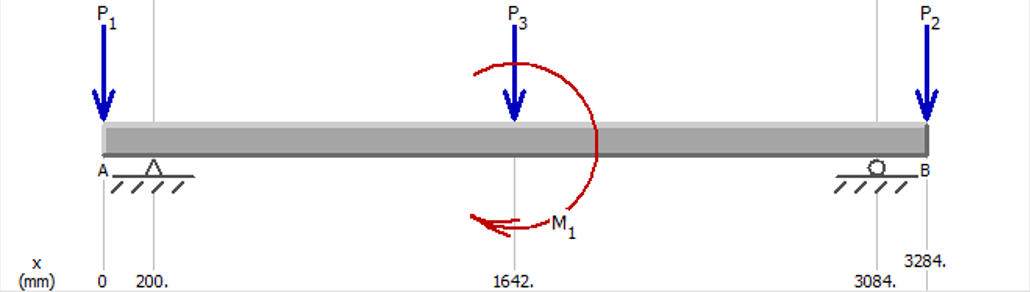
\includegraphics[width=\columnwidth]{imagenes/colectorDCL}
	\caption{Diagrama de cuerpo libre del eje del colector}
	\label{fig:colec1}
\end{figure}

Los resultados de la simulación se presentan en la Tabla \ref{tab:colec1}.

\begin{table}[H]
	\centering
	\caption{Resultados de la simulación}
	\begin{tabular}{|l|l|l|l|}
		\hline
		\textbf{Carga $ P_1 $ y $ P_2 $} & \textbf{Carga $ P_3 $} & \textbf{Reacciones (N)} & \textbf{Momentos (N*m)} \\
		\hline \hline
		\multirow{3}[6]{*}{$ Fx $} & \multirow{3}[6]{*}{$ Fr $} & $ R_Ar=3682.94 $ & $ M_Ar=-338.33 $ \\
		\cline{3-4}          &       & $ R_Br=3973.63 $ & $ M_Br=-338.33 $ \\
		\cline{3-4}          &       &  & $ Mr_{MAX}=2,952.28 $ \\
		\hline
		\multirow{3}[6]{*}{$ Fy $} & \multirow{3}[6]{*}{$ Ftg $} & $ R_Atg=20321.08 $ & $ M_Atg=-2,392.2 $ \\
		\cline{3-4}          &       & $ R_Btg=20321.08 $ & $ M_Btg=-2,392.2 $ \\
		\cline{3-4}          &       &       & $ Mtg_{MAX}=9,663.03 $ \\
		\hline
	\end{tabular}%
	\label{tab:colec1}%
\end{table}%

El momento flexionante máximo de este eje resultó ser el siguiente:
\begin{equation}
M_f = \sqrt{Mr_{MAX}^2 + Mtg_{MAX}^2} = 10103.965\ N*m
\end{equation}

Finalmente, para el cálculo del diámetro del eje, se utilizó la ecuación de esfuerzo cortante máximo \cite{DDA10}, estableciendo para este eje el material \textbf{Aluminio 6061 T6}. La expresión del diámetro despejado es la siguiente:
\begin{equation}
d=\sqrt[3]{\frac{FS}{R_C}*\sqrt{\frac{M_f^2+M_t^2}{0.04}}}=72.322\ mm
\end{equation}

Así, se propone que el diámetro del eje del Colector sea de \textbf{75\ mm}.\\

\textbf{Chavetas de los ejes del movimiento de elevación}

Con base en la Tabla expuesta en \cite{DDA3} (página 495), se seleccionó una chaveta de perfil cuadrangular, dado que el diámetro del eje no excede las $ 6 \frac{1}{2}\ in $. Ya que el eje del Colector será de casi 3 in, la chaveta tendrá un ancho de $ \frac{3}{4}\ in $. El material de la chaveta será de acero al bajo carbón, con estirado en frío \textbf{AISI 1020}, con resistencia a la fluencia de \textbf{350 MPa}.

Tomando en cuenta el par al que estará sometido el eje del Colector ($ \tau =1500\ Nm= 13276.12\ lb*in$), se tiene que la longitud mínima de la chaveta debe de ser de:
\begin{eqnarray}
L_m=\frac{4\tau}{\sigma_{p}DH}=2.4\ in
\end{eqnarray}

Así, se establece que el largo de la chaveta sea de \textbf{3\ in}.\\

\textbf{Anillos de retención del eje del Colector}

Considerando que el eje del Colector será de 3 in, se seleccionó en \cite{DDA4} el anillo de retención $ MSH-75 $, el cual es un anillo de eje para ensamble externo métrico ANSI. Este tendrá la función de sostener la corona de Elevación para evitar su desplazamiento axial en el eje.\\

\textbf{Rodamientos de los ejes del movimiento de elevación}

La selección de rodamientos se realizó con base en \cite{DDA5}. Para ello, se requiere conocer la carga resultante que tendrá cada uno de estos. De los resultados de la Tabla \ref{tab:colec1}, se calcularon las cargas máximas que tendrá que soportar cada rodamiento.
\begin{equation}
R_A=\sqrt{R_{Atg}^2+R_{Ar}^2}= 20.652\ kN
\end{equation}
\begin{equation}
R_B=\sqrt{R_{Btg}^2+R_{Br}^2}= 20.706\ kN
\end{equation}

Observando que ambos rodamientos tendrán la misma carga, se verificó que los rodamientos soporten al menos $ 20.7\ kN $. Para esto, se seleccionó la chumacera $ SN 617 $ con rodamiento de bolas autolineantes $ 1317 K $, el cual soporta hasta $ 38\ kN $.

Para soportar el eje del tornillo sinfín de elevación se seleccionó, con base en su diámetro, la chumacera $ SN 507 $ con rodamiento de bolas autolineantes $ 1207 K $, el cual soporta una carga máxima de $ 5.1\ kN $.\\

\textbf{\textit{Encoder del motor del movimiento de elevación}}

Este sensor es del mismo que se mencionó en el Módulo de Movimiento Azimutal. Los criterios de selección fueron los mostrados en el árbol de decisiones de la Figura \ref{fig:encoder1}.\\

\textbf{\textit{Sensor de final de carrera del movimiento de elevación}}

Se consideraron los mismos criterios del árbol de decisiones de la Figura \ref{fig:limitZ} para la selección de este sensor. La variante es que en este módulo se requiere un interruptor largo. Para cumplir esto, se consideraron los sensores de fin de carrera de la familia \textit{Actuador giratorio lateral de varilla ajustable}. Utilizando criterios de selección por medio de la herramienta AHP, tales como el precio, grado de protección industrial, tamaño, material del dispositivo y facilidad de fijación al mecanismo del módulo, el sensor seleccionado fue el siguiente: \underline{\textit{AEM2G7120Z11M}}. Sus características eléctricas se muestran en la Tabla \ref{tabla:caracteristicas} \cite{DDA8}.

\subsubsection{Modelado del sistema robótico}
Hasta este punto, ya se cuenta con el diseño de los módulos estructural y de seguimiento solar, por lo tanto, ya es posible describir a detalle el movimiento que produciría el seguidor solar al ponerse en marcha los motores eléctricos de azimutal y elevación. Este movimiento puede ser obtenido y descrito por medio del modelado matemático, considerando el tipo de movimiento a realizar, los elementos que ejecutan estos movimientos, la forma en cómo se transmite el movimiento a toda la estructura del seguidor y los grados de libertad que posee el seguidor. Todo esto se puede considerar al asimilar el sistema completo como un robot, cuya estructura representa su morfología, mientras que los módulos de movimiento azimutal y elevación proporcionan los mecanismos y elementos para generar el movimiento del robot.

El modelado es indispensable, ya que más adelante se describirá el algoritmo de seguimiento solar, el cual se encarga de generar trayectorias de movimiento para el seguidor. Se deberá respetar el error de seguimiento establecido en los requerimientos, lo que implica implementar un control para los motores que ejecutan los movimientos azimutal y de elevación, así que el modelado deberá considerar la dinámica del robot y de los motores eléctricos.

El modelado comienza con la identificación de la morfología del robot, para definir la cantidad de GDL y el tipo de juntas que posee. Hecho esto, se procede a establecer los marcos del robot, los cuales fueron colocados siguiendo la convención de Denavit-Hartenberg, para más detalles consultar \cite{DDA11}. El esquema del robot se muestra en la Figura \ref{fig:modelo1}, donde se observan los marcos de cada eslabón y las variables de cada junta, así como las distancias entre juntas y el tipo de movimiento de cada junta.

\begin{figure}[H]
	\centering
	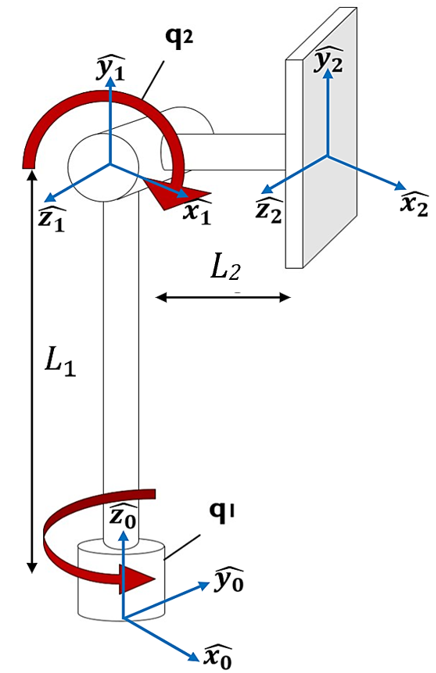
\includegraphics[width=5cm]{imagenes/modelo1}
	\caption{Esquema del robot seguidor solar.}
	\label{fig:modelo1}
\end{figure}

En este apartado se describen los resultados del modelo dinámico del robot, el cual se obtuvo siguiendo la teoría presentada en \cite{DDA11} y \cite{DDA12}. El modelado completo se encuentra en el Apéndice X. Se comenzó por obtener las ecuaciones de la dinámica del robot seguidor. El modelo dinámico en forma matricial se obtiene de acuerdo con la Ecuación (\ref{eq:modelo1}).
\begin{equation} \label{eq:modelo1}
    D(\textbf{q})\Ddot{\textbf{q}}+C(\textbf{q},\Dot{\textbf{q}})\Dot{\textbf{q}}+G(\textbf{q})=\textbf{u}-\bm{\tau_d}
\end{equation}

Donde $ n $ es el número de variables de junta (o GDL), \boldsymbol{$ q $} es el vector de $ nx1 $ con las variables de junta $ ( q_1,q_2,…,q_n ) $, \boldsymbol{$ u $} es el vector de $ nx1 $ con las fuerzas generalizadas que actúan en las juntas, $ D $ es la matriz de inercia, $ C $ es la matriz de Coriolis, $ G $ es la matriz de gravedad, y \boldsymbol{$ \tau_d $} es el vector de $ nx1 $ con los torques perturbadores en las juntas.

El cálculo de la matriz D requiere conocer el tensor de inercia y la masa de cada eslabón, por lo que se recurrió a SolidWorks para obtener esta información. La pista de movimiento y el tubo de soporte principal no son movidos por el robot, así que sus masas e inercias no influyen en el modelado robótico. En SolidWorks se construyeron subensambles excluyendo estos dos elementos, con el fin de obtener las masas e inercias aproximadas de cada eslabón. Esta información se muestra en la Figura \ref{fig:modelo2}, donde se observa que los valores de los elementos de los tensores de inercia de cada eslabón fuera de la diagonal principal son muy pequeños, por lo que se optó por no considerarlos para fines de simplificación del modelo dinámico, resultando así matrices diagonales de los tensores de inercia.

\begin{figure}[H]
	\centering
	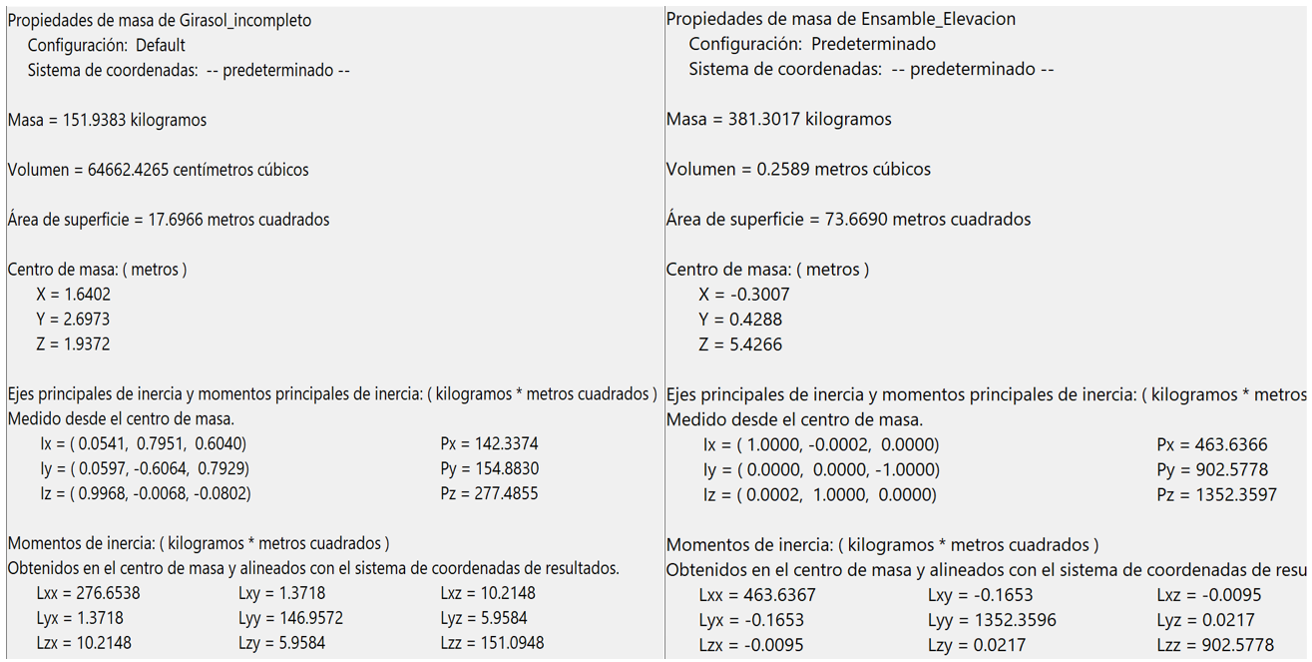
\includegraphics[width=\columnwidth]{imagenes/modelo2}
	\caption{Masas e inercias del eslabón azimutal (izquierda) y elevación (derecha).}
	\label{fig:modelo2}
\end{figure}

De forma similar, se calcularon las posiciones aproximadas de los centros de masa de cada eslabón y las distancias aproximadas entre cada motor, con base en la información proporcionada por la estructura diseñada en \textit{SolidWorks}. Posteriormente, se obtuvieron las matrices del modelo dinámico para el robot seguidor, utilizando el software de cálculo simbólico \textit{Mathematica}, el cual generó los resultados mostrados en las Ecuaciones (\ref{eq:modelo2}), (\ref{eq:modelo3}) y (\ref{eq:modelo4}). Se utilizó la siguiente notación simplificada para las funciones trigonométricas:
\begin{equation}
    sen(q_1)=S_1;\ sen(q_2)=S_2;\ cos(q_1)=C_1;\ cos(q_2)=C_2
\end{equation}
Elementos de la matriz de inercia:
\begin{equation}
    d_{11}= \frac{1}{2} \left(m_2 L_{cm2}^2+2I_{1y}+I_{2x}+I_{2y}+(m_2 L_{cm2}^2-I_{2x}+I_{2y})cos(2q_2)\right)
\end{equation}
\begin{equation}
    d_{12}=(I_{2x}-I_{2y})C_2 S_1 S_2
\end{equation}
\begin{equation}
    d_{21}=(I_{2x}-I_{2y})C_2 S_1 S_2
\end{equation}
\begin{equation}
    d_{22}=I_{2z} (C_1)^2+ \frac{1}{2}\left(2m_2 (L_{cm2})^2+I_{2y}-I_{2y}cos(2q_1)\right) (S_2)^2+\left(m_2 (L_{cm2})^2+I_{2x} (S_1)^2 \right)(C_2)^2
\end{equation}
\begin{equation} \label{eq:modelo2}
    D(\textbf{q})=
    \begin{bmatrix}
        d_{11} & d_{12} \\
        d_{21} & d_{22} 
    \end{bmatrix}
\end{equation}
Elementos de la matriz de Coriolis:
\begin{equation}
    c_{11}=(-m_2 L_{cm2}^2+I_{2x}-I_{2y} ) C_2 S_2 \Dot{q}_2
\end{equation}
\begin{multline*}
    c_{12}=(-m_2 L_{cm2}^2+I_{2x}-I_{2y} ) C_2 S_2 \Dot{q}_1 +\frac{1}{4} ((I_{2x}+I_{2y}-2I_{2z} )sen(2q_1 )\\
    +(I_{2x}-I_{2y} )cos(2q_2 )(sen(2q_1 )-4S_1 ))\Dot{q}_2
\end{multline*}
\begin{multline*}
    c_{21}= \frac{1}{2}(m_2 L_{cm2}^2-I_{2x}+I_{2y}+(I_{2x}-I_{2y}) C_1 )sen(2q_2) \Dot{q}_1 +\frac{1}{4}(I_{2x}+I_{2y}-2I_{2z})\\
    +(I_{2x}-I_{2y}(cos(2q_2 ) )sen(2q_1)\Dot{q}_2
\end{multline*}
\begin{equation}
    c_{22}=(I_{2y}-I_{2x} ) C_2 S_2 \Dot{q}_2 S_1^2+ \frac{1}{4} (I_{2x}+I_{2y}-2I_{2z}+(I_{2x}-I_{2y} )cos(2q_2 ) )sen(2q_1)\Dot{q}_1 )
\end{equation}
\begin{equation} \label{eq:modelo3}
    C(\textbf{q},\Dot{\textbf{q}})=
    \begin{bmatrix}
        c_{11} & c_{12} \\
        c_{21} & c_{22} 
    \end{bmatrix}
\end{equation}
Matriz de gravedad:
\begin{equation} \label{eq:modelo4}
    G(\textbf{q})=
    \begin{bmatrix}
        0 \\
        m_2 gL_{cm2} C_2 
    \end{bmatrix}
\end{equation}

En la Tabla \ref{tab:modelo1} se presentan todos los parámetros físicos que posee el robot seguidor, los cuales serán necesarios para la simulación del modelo dinámico y su posterior control.

\begin{table}[H]
  \centering
  \caption{Parámetros físicos del seguidor solar obtenidos de SolidWorks.}
    \begin{tabular}{|l|c|c|}
    \hline
    Parámetro & Valor & Unidades \\
    \hline
    $ I_{1x} $: Inercia respecto al eje x del eslabón 1 & 276.66 & $ kg*m^2 $ \\
    \hline
    $ I_{1y} $: Inercia respecto al eje y del eslabón 1 & 147 & $ kg*m^2 $ \\
    \hline
    $ I_{1z} $: Inercia respecto al eje z del eslabón 1 & 151.1 & $ kg*m^2 $ \\
    \hline
    $ I_{2x} $: Inercia respecto al eje x del eslabón 2 & 463.64 & $ kg*m^2 $ \\
    \hline
    $ I_{2y} $: Inercia respecto al eje y del eslabón 2 & 1352.36 & $ kg*m^2 $ \\
    \hline
    $ I_{2z} $: Inercia respecto al eje z del eslabón 2 & 902.58 & $ kg*m^2 $ \\
    \hline
    $ L_0 $: Distancia del suelo a la primera junta & 2.618 & $ m $ \\
    \hline
    $ L_1 $: Distancia de la primera junta a la segunda & 0.382 & $ m $ \\
    \hline
    $ L_2 $: Distancia de la segunda junta al punto más alejado del colector & 0.3 & $ m $ \\
    \hline
    $ L_{cm1} $: Distancia desde la primera junta al centro de masa del eslabón 1 & 0.191 & $ m $ \\
    \hline
    $ L_{cm2} $: Distancia desde la segunda junta al centro de masa del eslabón 2 & 0.297 & $ m $ \\
    \hline
    $ m_1 $: Masa del eslabón 1 & 152 & $ kg $ \\
    \hline
    $ m_2 $: Masa del eslabón 2 & 382 & $ kg $ \\
    \hline
    $ g $: Aceleración de la gravedad & 9.81 & $ \frac{m}{s^2} $ \\
    \hline
    \end{tabular}%
  \label{tab:modelo1}%
\end{table}%

El siguiente paso es obtener la dinámica del elemento encargado de realizar el movimiento de cada junta, en este caso los motores eléctricos mencionados en el módulo de seguimiento solar. Cada motor a utilizar puede modelarse con un circuito eléctrico y un sistema mecánico acoplado. La Figura \ref{fig:modelo3} muestra un esquema de la composición del modelo del motor de CD, el cual considera la transmisión mecánica y la carga acopladas al eje del motor.

\begin{figure}[H]
	\centering
	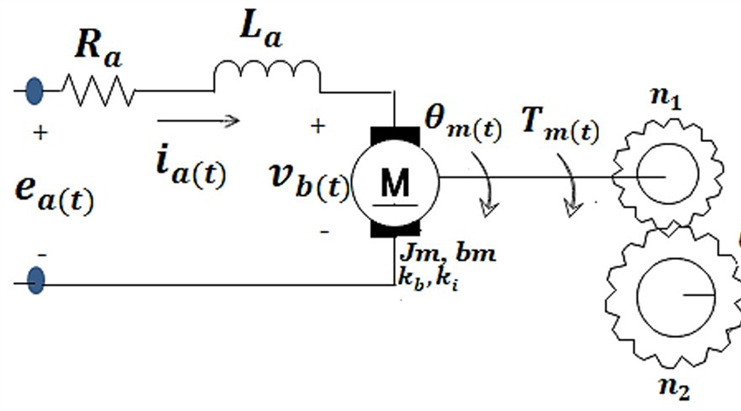
\includegraphics[width=10cm]{imagenes/modelo3}
	\caption{Esquema del modelo ideal del motor de CD.}
	\label{fig:modelo3}
\end{figure}

La entrada a este modelo es una tensión eléctrica, mientras que la salida es la posición angular del motor, afectada por la relación de reducción de la transmisión (dicha transmisión es el sinfín-corona diseñado anteriormente), la cual se representa con dos engranes. La salida $ \theta_L $ será la posición angular de una de las juntas del robot. En este modelo se logró considerar el efecto de las inercias y fricciones viscosas del motor, su eje y su transmisión, así como crear una relación directa entre la tensión aplicada y la posición angular de salida. La intención es implementar una estrategia de control a esta tensión de entrada para manipular la posición angular de la junta en función de la trayectoria de referencia (dada por el algoritmo de seguimiento solar o por las posiciones angulares ingresadas por el usuario desde una interfaz).

El análisis matemático del modelo ideal del motor de CD se puede consultar en \cite{DDA11} y \cite{DDA13}. En este apartado se presentan las ecuaciones resultantes de dicho análisis y el significado y valor de los parámetros físicos para este trabajo. Debido a que se utilizó el mismo motor para el movimiento azimutal y de elevación, los parámetros físicos serán iguales para ambas juntas, con excepción de $ J_m $, cuyo valor depende de la inercia del rotor del motor y la inercia de la transmisión mecánica, la cual no es la misma para ambas juntas.

El modelado del motor considera dos entradas, la tensión y la carga externa, por lo que la dinámica de dicho motor resultará de considerar ambos efectos, utilizando el principio de superposición. Para efectos de simplificación, se consideró que la constante de tiempo eléctrica es mucho menor que la constante de tiempo mecánica del motor, es decir: $ \frac{L}{R} \ll \frac{J_m}{B_m} $. Con estas consideraciones, se obtuvo el modelo dinámico del motor de CD, el cual es descrito por la Ecuación (\ref{eq:modelo5}).
\begin{equation} \label{eq:modelo5}
    J_m \Ddot{\theta}_m+\left(B_m+\frac{K_b K_i}{R}\right) \Dot{\theta}_m=\frac{K_i}{R}V-\frac{\tau_L}{r}
\end{equation}

Donde $ J_m $ es la inercia del rotor del motor y su transmisión mecánica, $ B_m $ es la fricción viscosa del motor, $ K_i $ es la constante de torque del motor, $ K_b $ es la constante de fueza contraelectromotriz del motor, $ R $ es la resistencia de armadura del motor, $ r $ es el factor de reducción de la transmisión mecánica, $ \Dot{\theta} $ es la posición angular del eje del motor, $ \tau_L $ es el torque producido por la carga acoplada al motor, y $ V $ es el voltaje de armadura del motor.

El torque $ \tau_L $ actúa en cada junta, convirtiéndose en la entrada de la Ecuación (\ref{eq:modelo1}), por lo tanto: $ u=[\tau_{L1},\tau_{L2}]^T $. Con esto, ya es posible combinar las Ecuaciones (\ref{eq:modelo1}) y (\ref{eq:modelo5}) para obtener la dinámica completa del sistema robótico, es decir, la dinámica del propio robot junto con la dinámica del motor de movimiento de cada junta. Debido a que el torque y el movimiento de cada junta puede ser diferente, es posible considerar ecuaciones independientes para cada junta del robot seguidor. La Ecuación (\ref{eq:modelo6}) representa la dinámica para la k-junta del robot, donde k=1,2,…,n, tomando en cuenta que, debido a la presencia de la transmisión, existe un factor de reducción que relaciona la variable angular del motor y la del robot de la siguiente forma: $ θ_{mk}=r_k q_k $.
\begin{equation} \label{eq:modelo6}
    (P^{-1} D(\textbf{q})+PJ)\Ddot{\textbf{q}} +(P^{-1} C(\textbf{q},\Dot{\textbf{q}})+PB)\Dot{\textbf{q}} +P^{-1} G(\textbf{q})=\textbf{U}-P^{-1}\bm{\tau_d}
\end{equation}
\begin{equation}
    P=
    \begin{bmatrix}
        r_1 & 0 \\
        0 & r_2 
    \end{bmatrix}
    ,\ J=
    \begin{bmatrix}
        J_{m1} & 0 \\
        0 & J_{m2}
    \end{bmatrix}
    ,\ B=
    \begin{bmatrix}
        B_{m1}+\frac{K_{b1} K_{i1}}{R_{k1}}  & 0 \\
        0 & B_{m2}+\frac{K_{b2} K_{i2}}{R_{k2}}
    \end{bmatrix}
    ,\ \textbf{U}=
    \begin{bmatrix}
        \frac{K_{i1}}{R_{1}}  & 0 \\
        0 & \frac{K_{i2}}{R_{2}}
    \end{bmatrix}
    \textbf{V}(t)
\end{equation}

Como se utilizará el mismo motor para ambas juntas, sus parámetros resultan ser los mismos para cualquiera de éstas, con excepción de $ J_m $, ya que las transmisiones no son iguales. Considerando lo anterior, la Ecuación (\ref{eq:modelo6}) se reduce a la Ecuación (\ref{eq:modelo7}).
\begin{equation} \label{eq:modelo7}
    \left(\frac{1}{r} D(\textbf{q})+rJ\right)\Ddot{\textbf{q}} +\left(\frac{1}{r} C(\textbf{q},\Dot{\textbf{q}})+r\left(B_m+\frac{K_i K_b}{R}\right) I_{2x2} \right)\Dot{\textbf{q}}+\frac{1}{r} G(\textbf{q})=\frac{K_i}{R} \textbf{V(t)}-\frac{\bm{\tau_d}}{r}
\end{equation}

Donde \boldsymbol{$ V(t) $} es un vector de $ nx1 $ con las entradas de tensión eléctrica a cada motor.

Los parámetros físicos del motor se obtuvieron del manual de uso general de motores de CD de IRONHORSE® \cite{DDA14}. Con la información dada por las curvas de desempeño se calcularon las constantes del motor y la fricción viscosa. La inercia del motor $ J_a $ y su resistencia de armadura $ R $ las proporciona directamente el manual. Estos parámetros fueron calculados utilizando las siguientes relaciones, considerando al motor en estado estacionario:

\begin{itemize}
    \item $ V_b=K_b \omega $ (relación entre voltaje y velocidad angular)
    \item $ \tau_m=K_i I_a $ (relación entre torque y corriente de armadura)
    \item $ V=V_b+RI_a $ (corriente de armadura constante)
    \item $ \tau_m=B_m \omega $ (motor sin carga acoplada)
\end{itemize}

Por último, para calcular $ J_m $ se obtuvieron de SolidWorks las inercias de las transmisiones, sumándolas a la inercia del motor. La Tabla \ref{tab:modelo2} resume los parámetros físicos del motor.

\begin{table}[H]
  \centering
  \caption{Parámetros físicos del motor.}
    \begin{tabular}{|c|c|c|}
    \hline
    \textbf{Parámetro} & \textbf{Valor} & \textbf{Unidades} \\
    \hline \hline
    $ J_a $  & 0.02365 & $ kg*m^2 $ \\
    \hline
    $ J_{m1} $  & 0.05305 & $ kg*m^2 $ \\
    \hline
    $ J_{m2} $  & 0.07135 & $ kg*m^2 $ \\
    \hline
    $ K_i $  & 0.4225 & $ N*m/A $ \\
    \hline
    $ K_b $  & 0.4808 & $ N*s/rad $ \\
    \hline
    $ B_m $  & 1.4683x10-3 & $ N*m*s $ \\
    \hline
    $ R $  & 1.31 & $ \Omega $ \\
    \hline
    $ r $  & 4800 & - \\
    \hline
    \end{tabular}%
  \label{tab:modelo2}%
\end{table}%

\subsubsection{Estrategia de control para el sistema robótico}
Antes de definir el controlador, se estableció el tipo de control a realizar, ya que es posible implementar un seguimiento continuo o punto a punto. Las condiciones de aplicación del seguidor solar permiten elegir el control por juntas independientes debido a que:

\begin{itemize}
    \item La trayectoria a seguir puede verse como una serie de puntos separados igualmente.
    \item El cambio de posición del Sol es muy lento, resultando más eficiente implementar un seguimiento punto a punto, en el cual no importaría mucho el perfil de la trayectoria.
    \item Los movimientos azimutal y de elevación son independientes en cuanto al camino o perfil de trayectoria que recorren.
    \item No es relevante el perfil de movimiento a realizar por cada junta, siendo más relevante la orientación final en cada punto de la trayectoria solar.
\end{itemize}

Este tipo de control permite tratar cada junta como un sistema individual, priorizando el alcanzar con el mínimo error cada punto de la trayectoria dada y dando poca importancia al error generado durante el camino entre el punto inicial y final.

El siguiente paso es definir el controlador a utilizar. Se consideraron el PD, PID y GPI por ser los más conocidos e implementados en sistemas robóticos. Cada uno posee ventajas y desventajas, por lo que fue necesario seleccionar el controlador mediante simulaciones.

En esta sección se presenta la linealización del sistema descrito por la Ecuación (\ref{eq:modelo7}) y las señales de control generadas por cada controlador. Para más información del análisis matemático de los controladores, consultar \cite{DDA11}, \cite{DDA12} y \cite{DDA15}. La Ecuación (\ref{eq:modelo7}) se puede reescribir como se muestra en la Ecuación (\ref{eq:modelo8}), de forma que los términos no lineales se separen de los lineales.
\begin{equation} \label{eq:modelo8}
    \left(J_{mk}+\frac{1}{r^2}d_{kk} (\textbf{q})\right)r\Ddot{q}_k+\left(B_m+\frac{K_b K_i}{R}\right)r\Dot{q}_k=\frac{K_i}{R} V_k (t)-d_k
\end{equation}
\begin{equation}
    Donde:\ d_k=\frac{1}{r}\left(\sum _{j \neq k}^{n}d_{kj} (\textbf{q})\Ddot{q}_j + \sum _{i,j=1}^{n}c_{ijk} (\textbf{q})\Dot{q}_i\Dot{q}_j +g_k +\tau_{dk}\right)
\end{equation}

Se observa que los términos no lineales están divididos por el factor de reducción, lo cual significa que a mayor reducción, menor será el efecto de las no linealidades. Bajo esta condición, es posible obtener un sistema equivalente lineal al cual se le puedan aplicar los controladores ya mencionados. Este nuevo sistema es descrito por la Ecuación (\ref{eq:modelo9}).
\begin{equation} \label{eq:modelo9}
    J_{eff} r\Ddot{q}_k+B_{eff} r\Dot{q}_k=U_k-d_k
\end{equation}
\begin{equation}
    Donde:\ U_k=\frac{K_i}{R}V_k (t),\ d \approx constante
\end{equation}

A partir de este punto se prescindirá del subíndice $ k $, asumiendo que las expresiones desarrolladas son aplicables para cualquiera de las juntas del robot. Con base en el sistema lineal (\ref{eq:modelo9}) se desarrollaron los 3 controladores a ser analizados, considerando una trayectoria de referencia suave con 2 derivadas continuas $ q^* (t) $, de forma que la trayectoria $ q(t) $ de cada junta se aproxime a la trayectoria de referencia, produciendo una señal de control \textit{u}.

Para este caso, las trayectorias serán construidas con un polinomio de interpolación cúbico, el cual permitirá definir la posición, velocidad y tiempo inicial y final de los dos puntos involucrados en cada paso de la trayectoria solar. Este polinomio posee la forma mostrada en la Ecuación (\ref{eq:modelo10}), mientras que la Ecuación (\ref{eq:modelo11}) representa en forma matricial la obtención de los coeficientes de dicho polinomio.
\begin{equation} \label{eq:modelo10}
    q^* (t)=a_0+a_1 t+a_2 t^2+a_3 t^3
\end{equation}
\begin{equation} \label{eq:modelo11}
    \begin{bmatrix}
        1 & t_0 & t_0^2 & t_0^3 \\
        0 & 1 & 2t_0 & 3t_0^2 \\
        1 & t_f & t_f^2 & t_f^3 \\
        0 & 1 & 2t_f & 3t_f^2
    \end{bmatrix}
    \begin{bmatrix}
        a_0 \\
        a_1 \\
        a_2 \\
        a_3
    \end{bmatrix}
    =
    \begin{bmatrix}
        q_0^* \\
        \Dot{q}_0^* \\
        q_f^* \\
        \Dot{q}_f^*
    \end{bmatrix}
\end{equation}

Donde $ q_0^* $ es la posición inicial de referencia, $ q_f^* $ es la posición final de referencia, $ t_0 $ es el tiempo en que ocurre la posición inicial, y $ t_f $ es el tiempo en que ocurre la posición final.

El valor de los tiempos inicial y final dependerá de la respuesta del controlador, ya que para intervalos muy pequeños podría requerirse más potencia de la que el motor puede suministrar. Para cualquier punto posterior al de inicio de la trayectoria, la posición final se volverá la posición inicial del siguiente paso, de manera que la trayectoria solar se construirá a través de funciones cúbicas que unirán los puntos generados por el algoritmo de seguimiento solar (modo automático), o los puntos ingresados desde la interfaz de usuario (modo manual).

Ya establecida la trayectoria de referencia, se presentan las señales de control generadas por cada controlador a analizar. La Ecuación (\ref{eq:modelo12}) muestra la señal de un controlador PD+FF, la Ecuación (\ref{eq:modelo13}) corresponde a la señal de un controlador PID+FF y la Ecuación (\ref{eq:modelo14}) describe la señal para un controlador GPI.
\begin{equation}
    u^*=rJ_{eff} \left(\Ddot{q}^*+\frac{B_{eff}}{J_{eff}}  \Dot{q}^*\right)
\end{equation}
\begin{equation} \label{eq:modelo12}
    u_{PD}=u^*-rJ_{eff} [K_d (\Dot{q} -\Dot{q}̇^* )+K_p (q-q^* )]
\end{equation}
\begin{equation} \label{eq:modelo13}
    u_{PID}=u^*-rJ_{eff} \left[K_d (\Dot{q} -\Dot{q}̇^* )+K_p (q-q^* +K_i \int(q-q^* ) \right]
\end{equation}
\begin{equation} \label{eq:modelo14}
    u_{GPI}=u^*-rJ_{eff} \left[k_3 (\Hat{\Dot{q}}- \Dot{q}^*)+k_2 (q-q^* )+k_1 \int(q-q^* ) +k_1 \iint(q-q^* ) \right]
\end{equation}

Se utilizó el entorno de MATLAB/Simulink para llevar a cabo las simulaciones de los 3 controladores propuestos. Con cada controlador se realizó una sintonización a prueba y error; posteriormente se determinó el tiempo de simulación ideal para cada caso de movimiento; después se agregó una perturbación al sistema y se ajustaron los parámetros; por último se compararon los resultados para las variables más importantes del sistema, dando mayor peso a aquellas involucradas en el error de seguimiento y el consumo energético. Las variables comparadas fueron: posiciones de las juntas ($ q_1,q_2 $), velocidades angulares de los motores ($ \omega_1,\omega_2 $), señales de control ($ V_1,V_2 $) y los torques demandados para cada motor ($ \tau_{m1},\tau_{m2} $). 

En la Tabla \ref{tab:control1} se presentan los parámetros de simulación para los 3 controladores, los cuales son los mismos para cada punto simulado, con el fin de obtener resultados lo más homogéneos posibles. Cabe mencionar que los valores de las ganancias mostrados en esta tabla son los mismos para ambas juntas.

\textbf{NOTA}: La entrada de perturbación corresponde a $ \tau_d $ y se asume que se presentará de forma intermitente, cuyo valor máximo permitido es el doble del valor del torque torsional ($ M_t $) en el eje del colector, es decir, de 3000 Nm. Esta perturbación se simula como una señal cuadrada periódica, representando así la intermitencia de su ocurrencia y el cambio abrupto que produciría en el sistema.

\begin{table}[H]
  \centering
  \caption{Parámetros generales de simulación de los controladores.}
    \begin{tabular}{|p{4.5cm}|ccc|}
    \hline
    \textbf{Parámetro} & \multicolumn{1}{p{1.5cm}|}{\textbf{PD+FF}} & \multicolumn{1}{p{1.5cm}|}{\textbf{PID+FF}} & \multicolumn{1}{p{1.5cm}|}{\textbf{GPI}} \\
    \hline \hline  
    Ganancias & \multicolumn{1}{p{1.5cm}|}{$ K_p=20 $ \newline{} $ K_d=10 $} & \multicolumn{1}{p{1.5cm}|}{$ K_p=20 $ \newline{} $ K_d=10 $ \newline{} $ K_i=1 $} & \multicolumn{1}{p{1.5cm}|}{$ K_p=2 $ \newline{} $ K_d=80 $ \newline{} $ K_i=30 $ \newline{} $ K_d=30 $} \\
    \hline
    Amplitud de perturbación & \multicolumn{3}{c|}{$ \tau_d=3000\ Nm $} \\
    \hline
    Periodo y \% de ancho de pulso de la señal de perturbación & \multicolumn{3}{p{3cm}|}{$ T=4\ s $ \newline{} $ ancho=20\% $} \\
    \hline
    Tiempo de respuesta para un paso de la trayectoria solar & \multicolumn{3}{c|}{$ t_p=20\ s $} \\
    \hline
    Tiempo de respuesta para el rango máximo de movimiento & \multicolumn{3}{c|}{$ t_{max}=180\ s $} \\
    \hline
    \end{tabular}%
  \label{tab:control1}%
\end{table}%

Se realizaron simulaciones para 3 puntos de movimiento, con el fin de analizar la respuesta y el desempeño de cada controlador. Se elaboró un programa en MATLAB para obtener los valores máximos de cada variable analizada, así como el error obtenido al final de la trayectoria. Esta información se despliega en una tabla en la ventana de comandos de MATLAB. Para cada punto se asumió una posición de 0° como punto de partida y para las condiciones iniciales de los integradores de las juntas del robot, es decir $ \textbf{q}(0)=[0°,0°]^T $. Las posiciones de estos puntos se encuentran en la Tabla \ref{tab:control2}.

\begin{table}[H]
  \centering
  \caption{Posiciones a simular para el análisis de los controladores.}
    \begin{tabular}{|l|c|c|}
    \hline
    \textbf{Punto} & \textbf{Posición de} $ q_1 $ & \textbf{Posición de} $ q_2 $ \\
    \hline
    Primer punto & 2.25° & 2.25° \\
    \hline
    Segundo punto & 9° & 9° \\
    \hline
    Tercer punto & 180° & 90° \\
    \hline
    \end{tabular}%
  \label{tab:control2}%
\end{table}

Es importante mencionar que el motor nunca debe operar en sus condiciones de trabajo máximas, las cuales son, de acuerdo con \cite{DDA1}, $ V=90\ V $, $ \omega=1800\ rpm $, $ \tau_m=1.97\ Nm $.

Para llevar a cabo la simulación, se construyeron los diagramas de bloques mostrados en las Figuras \ref{fig:control1}-\ref{fig:control3}, cada una correspondiendo a cada controlador. Así mismo, se muestran las ventanas desde las cuales se ingresan los diferentes datos necesarios para cada simulación.

\begin{figure}[H]
	\centering
	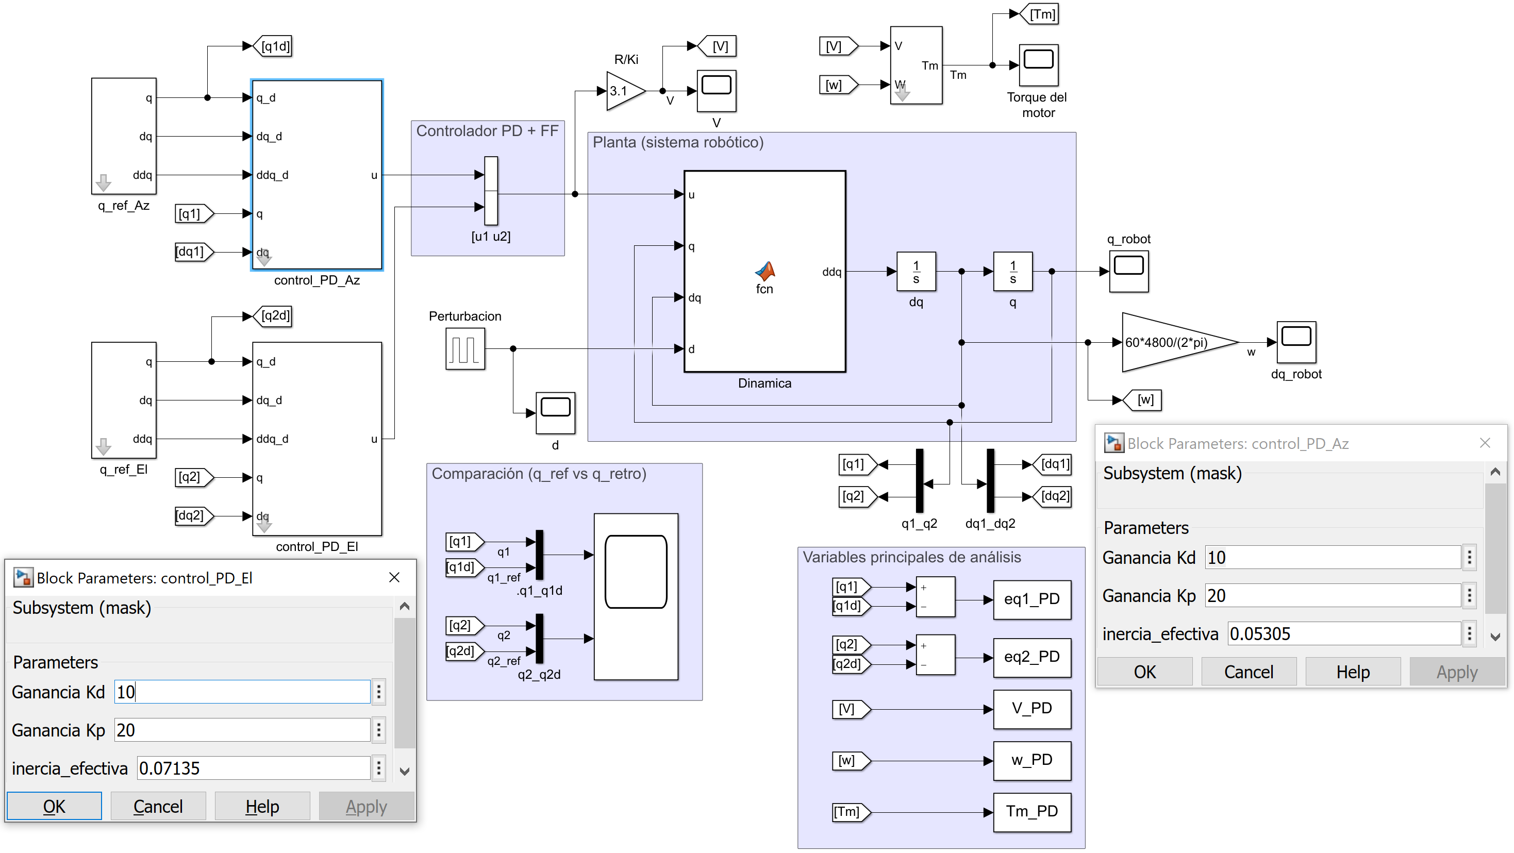
\includegraphics[width=\columnwidth]{imagenes/control1}
	\caption{Diagrama de bloques para el controlador PD usado en el sistema robótico.}
	\label{fig:control1}
\end{figure}

\begin{figure}[H]
	\centering
	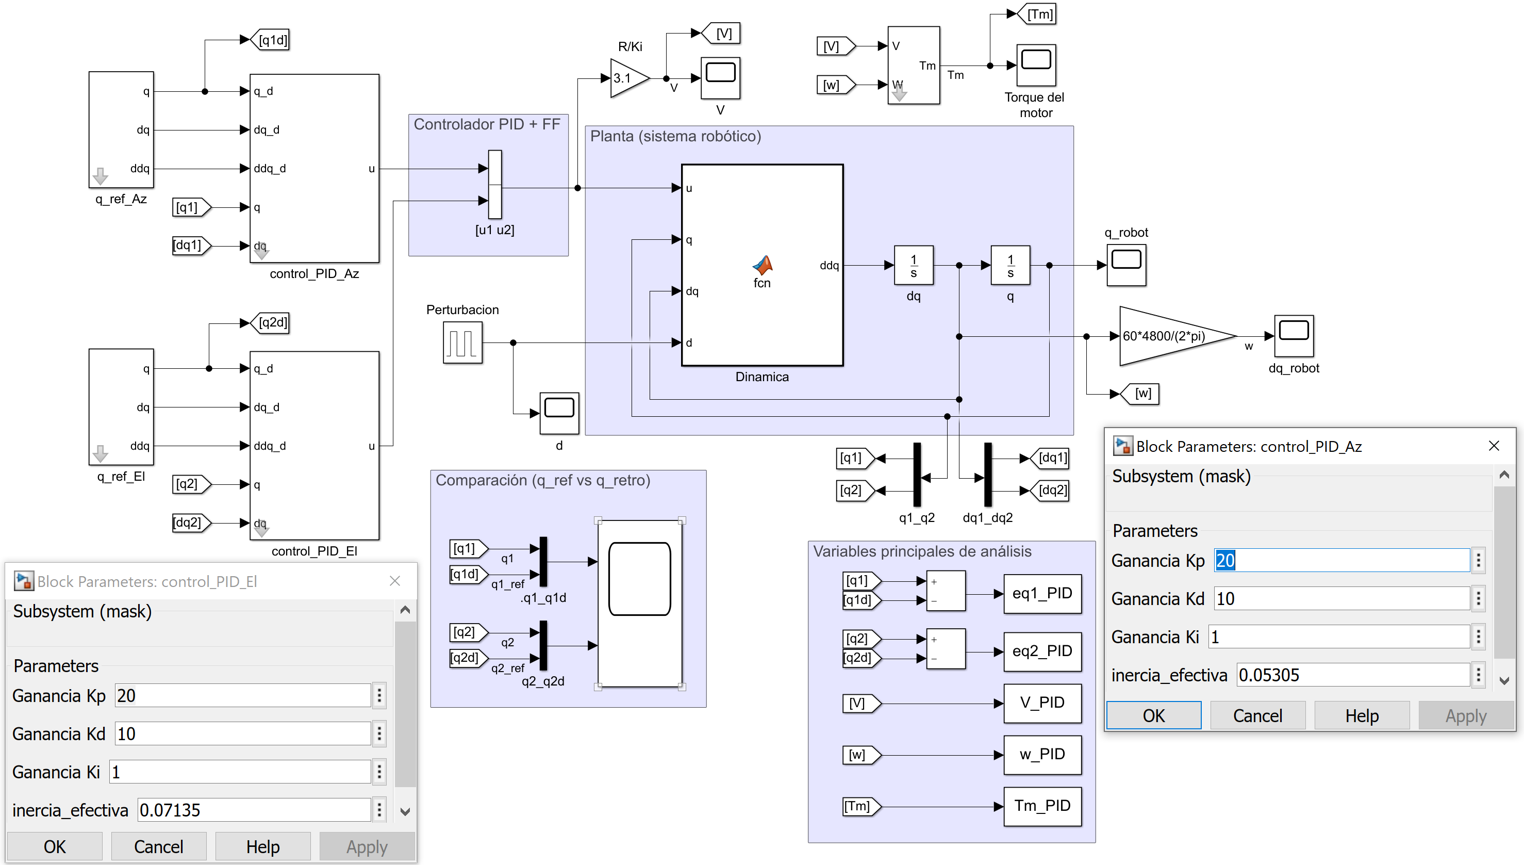
\includegraphics[width=\columnwidth]{imagenes/control2}
	\caption{Diagrama de bloques para el controlador PID usado en el sistema robótico.}
	\label{fig:control2}
\end{figure}

\begin{figure}[H]
	\centering
	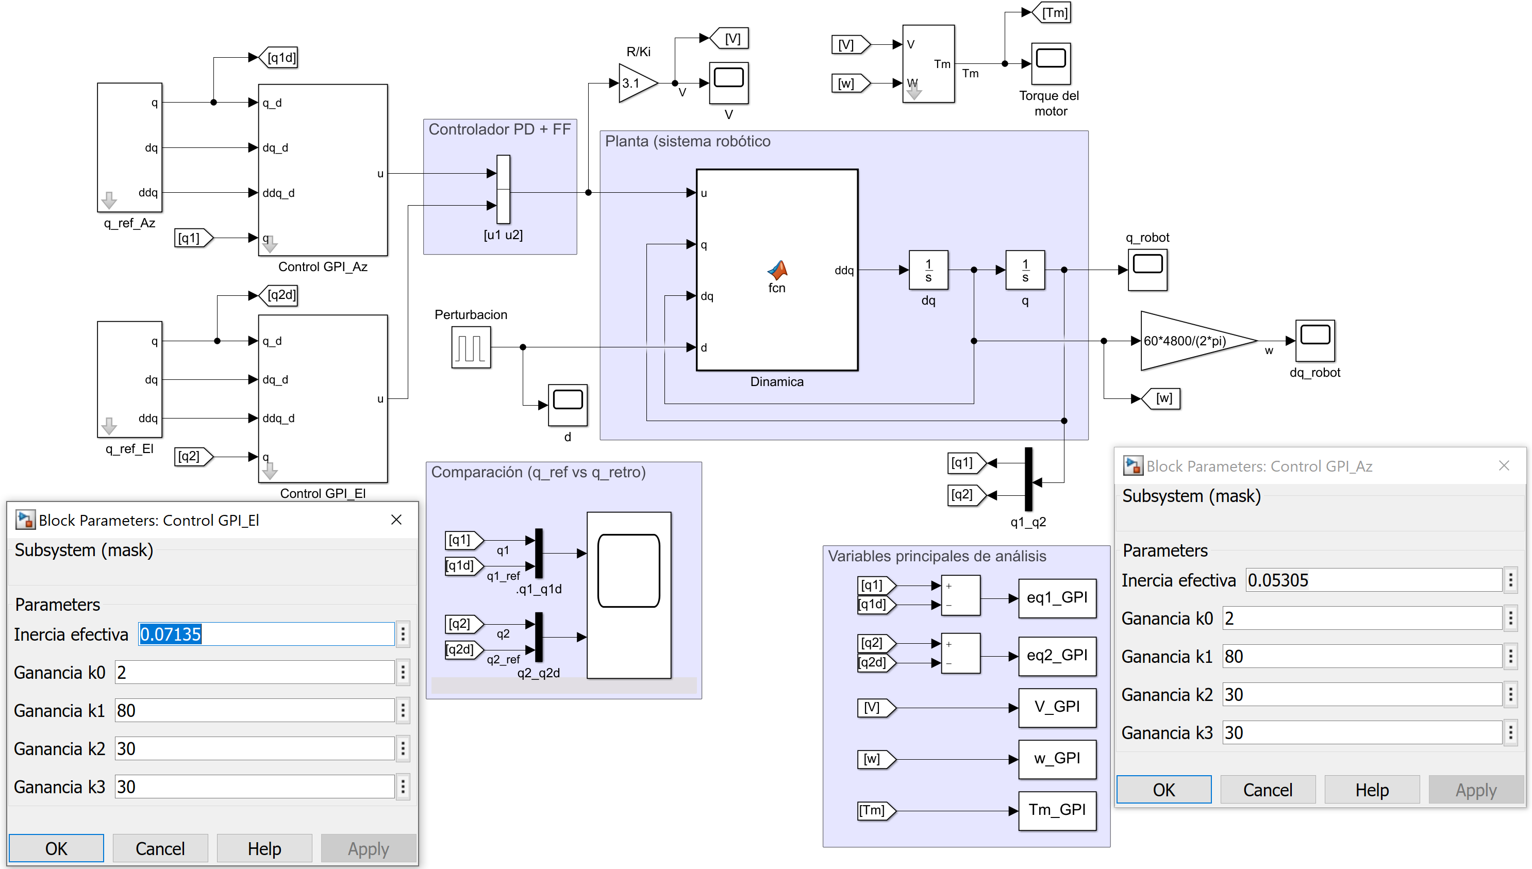
\includegraphics[width=\columnwidth]{imagenes/control3}
	\caption{Diagrama de bloques para el controlador GPI usado en el sistema robótico.}
	\label{fig:control3}
\end{figure}

Como se puede observar, al inicio de cada diagrama se encuentra el bloque que genera la trayectoria de referencia, cuyos valores de entrada dependerán del punto a analizar. Estos valores se solicitan a través de una ventana como la mostrada en la Figura \ref{fig:control4}. Por otro lado, se observa una sección con las variables principales, las cuales son enviadas al espacio de trabajo de MATLAB para ser procesadas en el programa que despliega la tabla de resultados.

\begin{figure}[H]
	\centering
	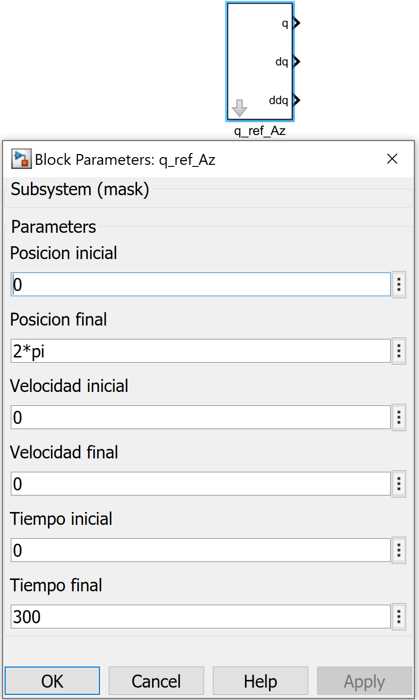
\includegraphics[width=4cm]{imagenes/control4}
	\caption{Valores requeridos por el bloque generador de la trayectoria de referencia.}
	\label{fig:control4}
\end{figure}

\begin{itemize}
    \item Primer punto\\
    En la Figura \ref{fig:control5} se muestran los valores obtenidos para las variables más importantes.
    \begin{figure}[H]
    	\centering
    	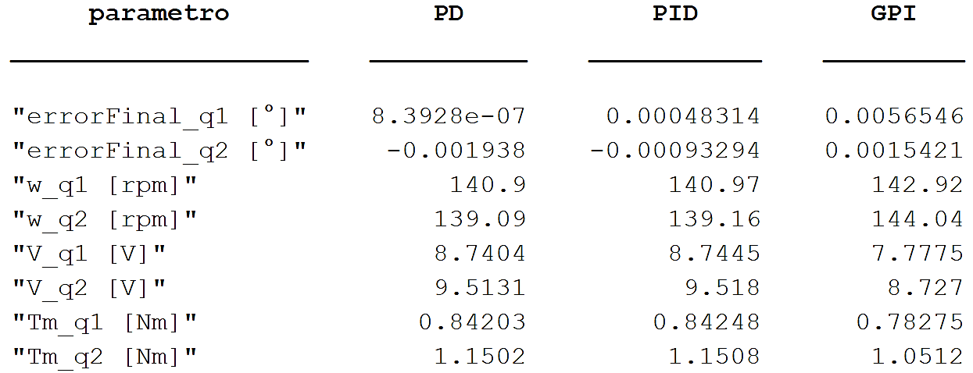
\includegraphics[width=11cm]{imagenes/control5}
    	\caption{Valores obtenidos para el primer punto de la simulación de los controladores.}
    	\label{fig:control5}
    \end{figure}
    La Figura \ref{fig:control6} presenta las curvas de posición de referencia y de la junta; la Figura \ref{fig:control7} muestra las curvas del voltaje de armadura; la Figura \ref{fig:control8} muestra las curvas del torque del motor y la Figura \ref{fig:control9} presenta las curvas de velocidad angular. La gráfica izquierda corresponde al controlador PD, la central al PID y la derecha al GPI.
    \begin{figure}[H]
    	\centering
    	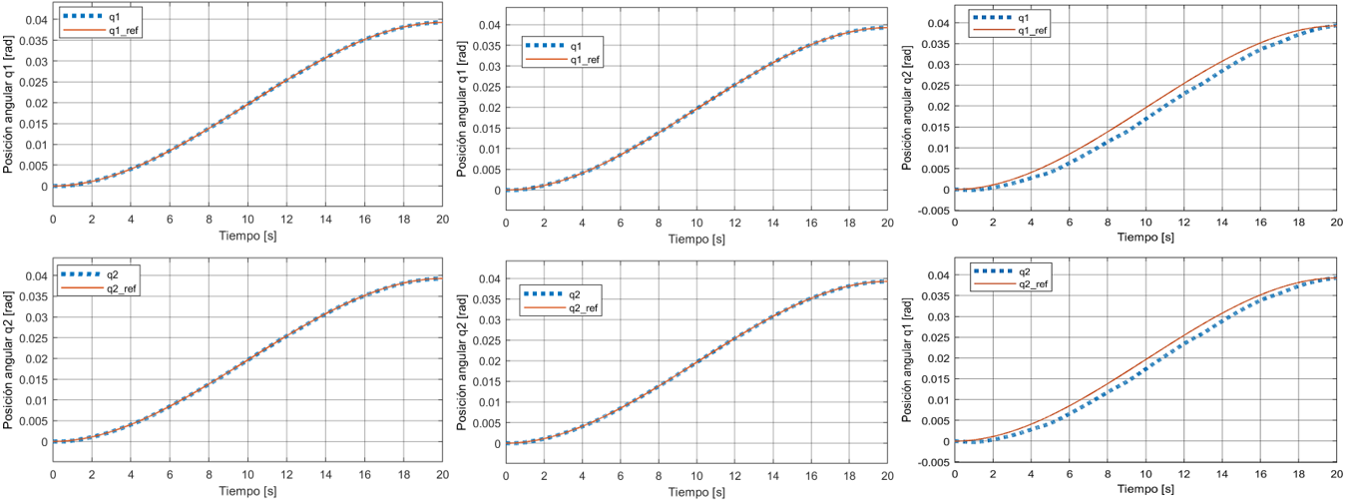
\includegraphics[width=\columnwidth]{imagenes/control6}
    	\caption{Gráficas de las posiciones de referencia y de la junta para el primer punto.}
    	\label{fig:control6}
    \end{figure}
    \begin{figure}[H]
    	\centering
    	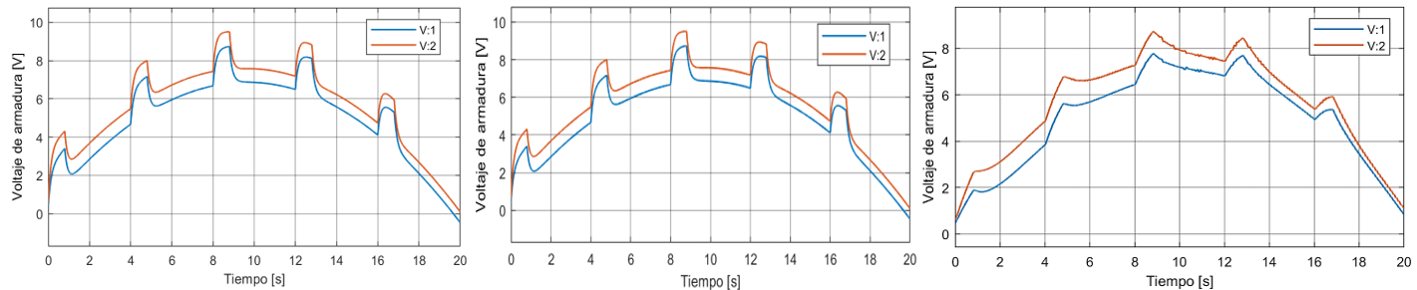
\includegraphics[width=\columnwidth]{imagenes/control7}
    	\caption{Gráficas de los voltajes de armadura para el primer punto.}
    	\label{fig:control7}
    \end{figure}
    \begin{figure}[H]
    	\centering
    	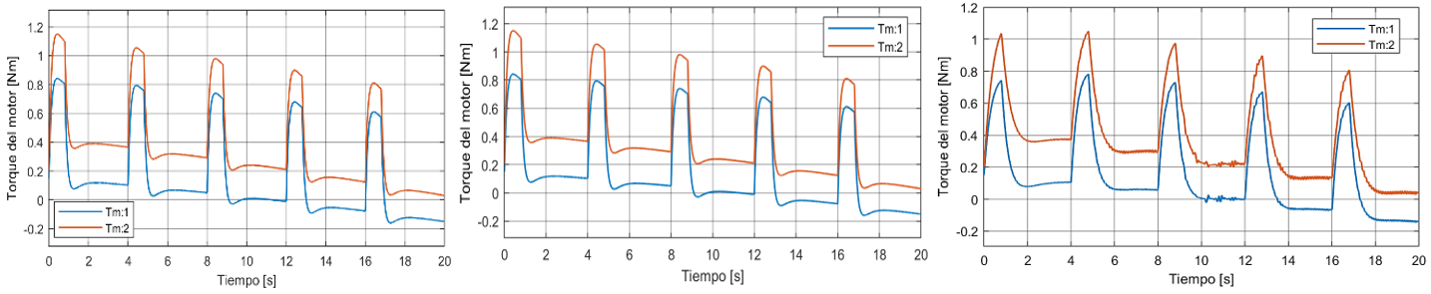
\includegraphics[width=\columnwidth]{imagenes/control8}
    	\caption{Gráficas de los torques demandados para los motores para el primer punto.}
    	\label{fig:control8}
    \end{figure}
    \begin{figure}[H]
    	\centering
    	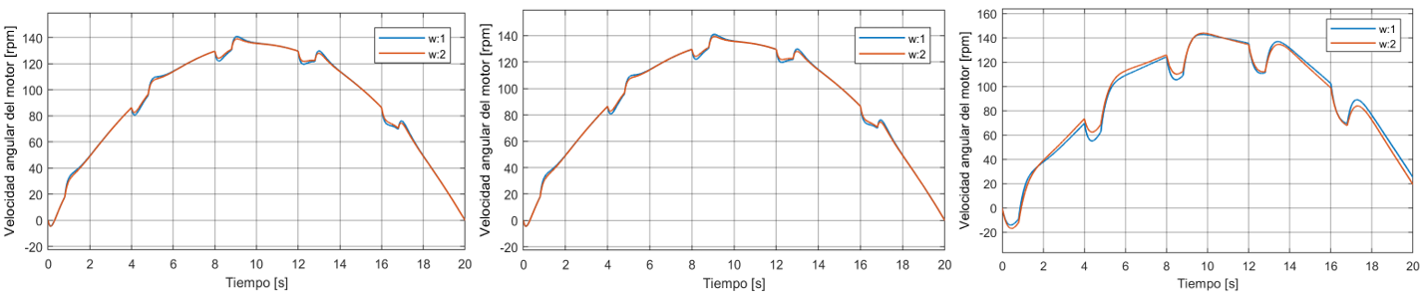
\includegraphics[width=\columnwidth]{imagenes/control9}
    	\caption{Gráficas de las velocidades angulares de los motores para el primer punto.}
    	\label{fig:control9}
    \end{figure}
    Se observa que el GPI es el que mayor error posee, aunque también es el que menor torque y voltaje de armadura requiere. Se debe considerar el hecho de que los errores teóricos obtenidos serán imposibles de lograr en la implementación física, resaltando que todos los controladores son capaces de alcanzar un error menor a 1°. Además, ningún controlador exige valores cercanos a los máximos soportados por el motor.\\
    Debido a su complejidad, el GPI parecería la última opción, pero el que requiera menor voltaje y torque implica una reducción del consumo energético, lo cual permite considerarlo seriamente como opción final.
    \item Segundo punto\\
    En la Figura \ref{fig:control10} se muestran los valores obtenidos para las variables más importantes.
    \begin{figure}[H]
    	\centering
    	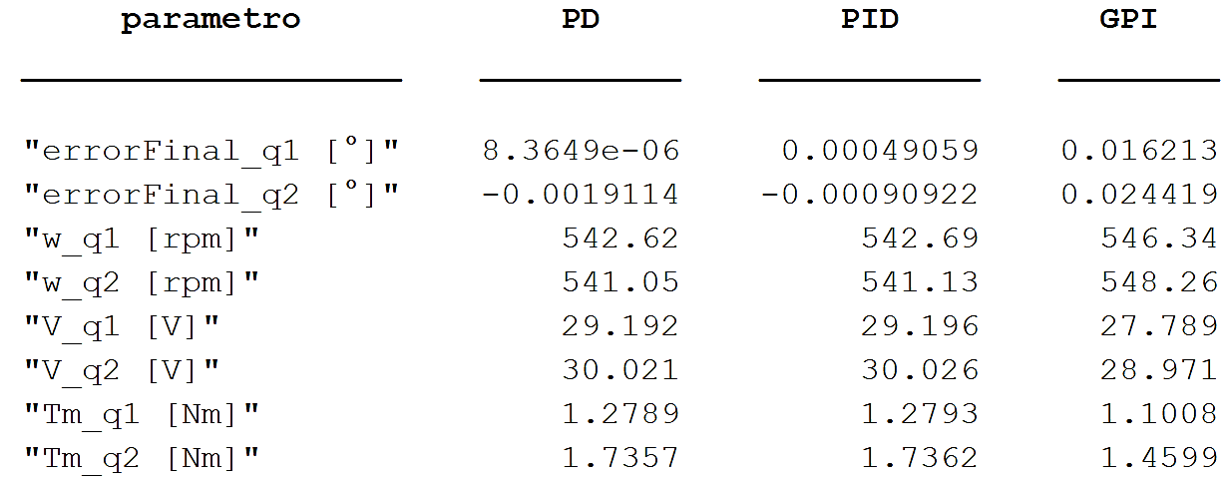
\includegraphics[width=10cm]{imagenes/control10}
    	\caption{Valores obtenidos para el segundo punto de la simulación de los controladores.}
    	\label{fig:control10}
    \end{figure}
    \begin{figure}[H]
    	\centering
    	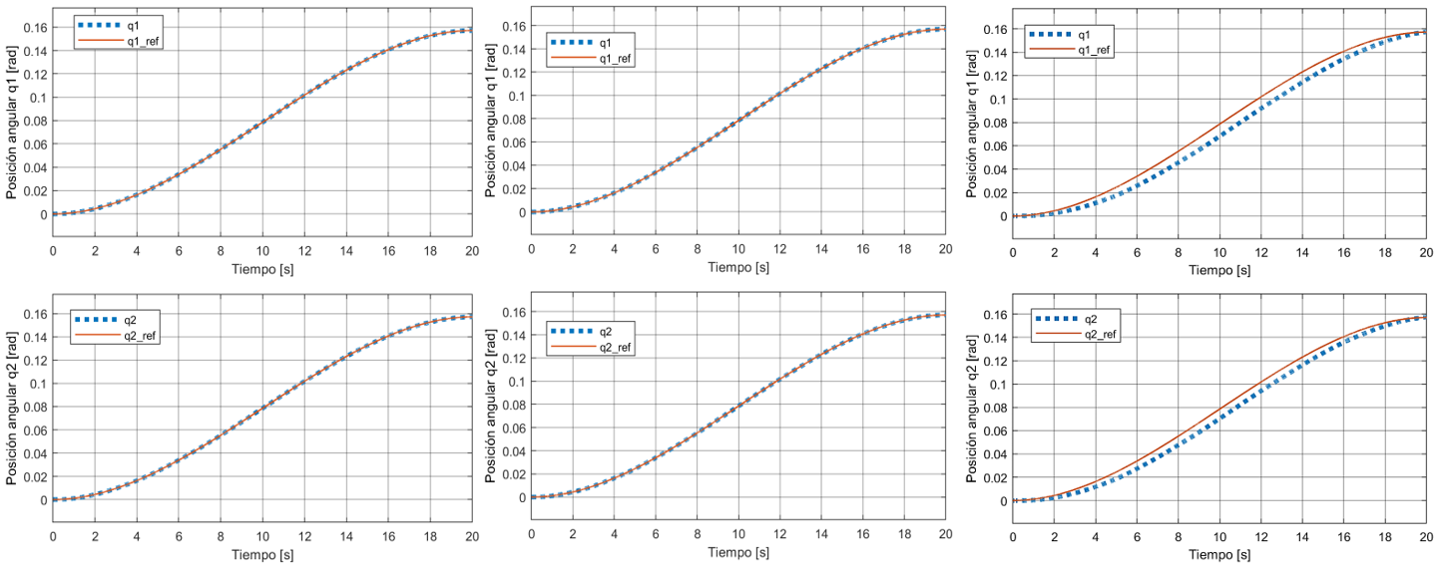
\includegraphics[width=\columnwidth]{imagenes/control11}
    	\caption{Gráficas de las posiciones de referencia y de la junta para el segundo punto.}
    	\label{fig:control11}
    \end{figure}
    \begin{figure}[H]
    	\centering
    	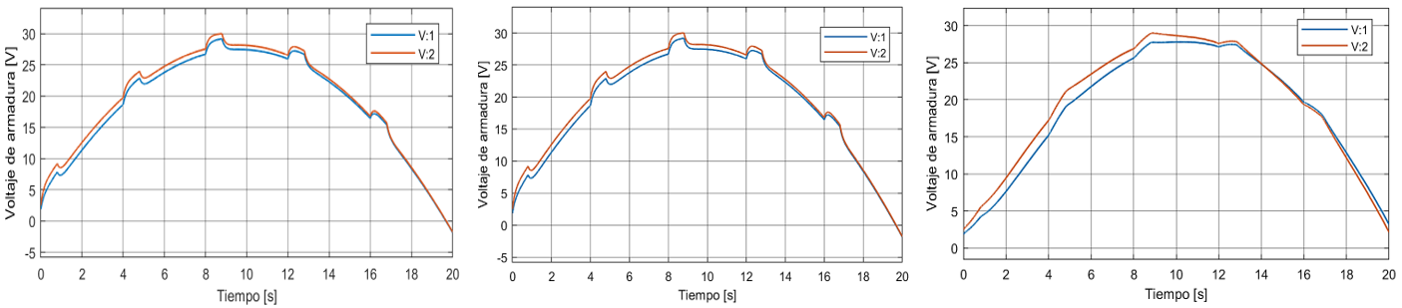
\includegraphics[width=\columnwidth]{imagenes/control12}
    	\caption{Gráficas de los voltajes de armadura para el segundo punto.}
    	\label{fig:control12}
    \end{figure}
    \begin{figure}[H]
    	\centering
    	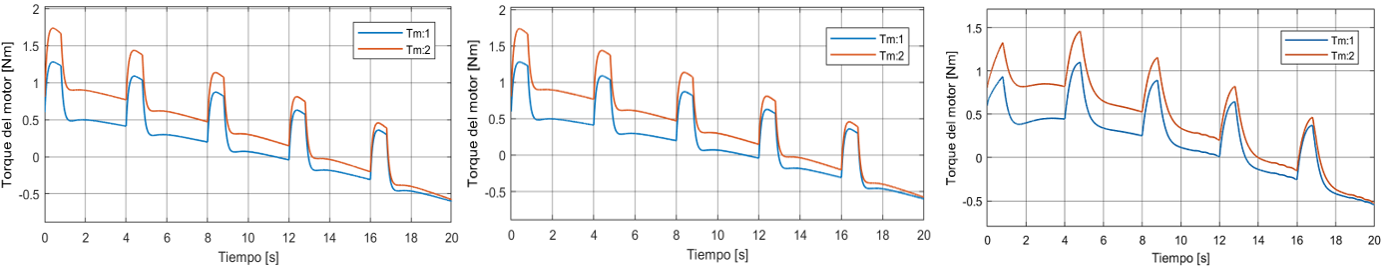
\includegraphics[width=\columnwidth]{imagenes/control13}
    	\caption{Gráficas de los torques demandados para los motores para el segundo punto.}
    	\label{fig:control13}
    \end{figure}
    \begin{figure}[H]
    	\centering
    	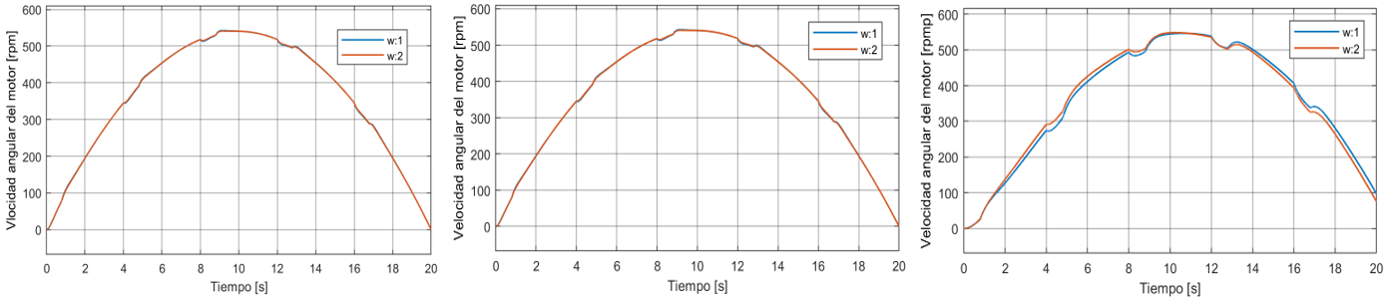
\includegraphics[width=\columnwidth]{imagenes/control14}
    	\caption{Gráficas de las velocidades angulares de los motores para el segundo punto.}
    	\label{fig:control14}
    \end{figure}
    En las Figuras \ref{fig:control11}-\ref{fig:control14} se muestran las gráficas para las posiciones, voltajes de armadura, torques y velocidades angulares, de la misma forma que en el primer punto. Los resultados para este punto son similares al primer punto, el GPI mantiene un error superior al PD y PID, pero demanda menos voltaje de armadura y torque. Para la junta de $ q_2 $ ya se hace notoria la diferencia en el torque, lo que implica un mayor ahorro de energía por parte del GPI. Considerando que el error alcanzado por el GPI sigue siendo inferior a 1°, la idea de optar por este controlador se vuelve más sólida.
    \item Tercer punto\\
    En la Figura \ref{fig:control15} se muestran los valores obtenidos para las variables más importantes.
    \begin{figure}[H]
    	\centering
    	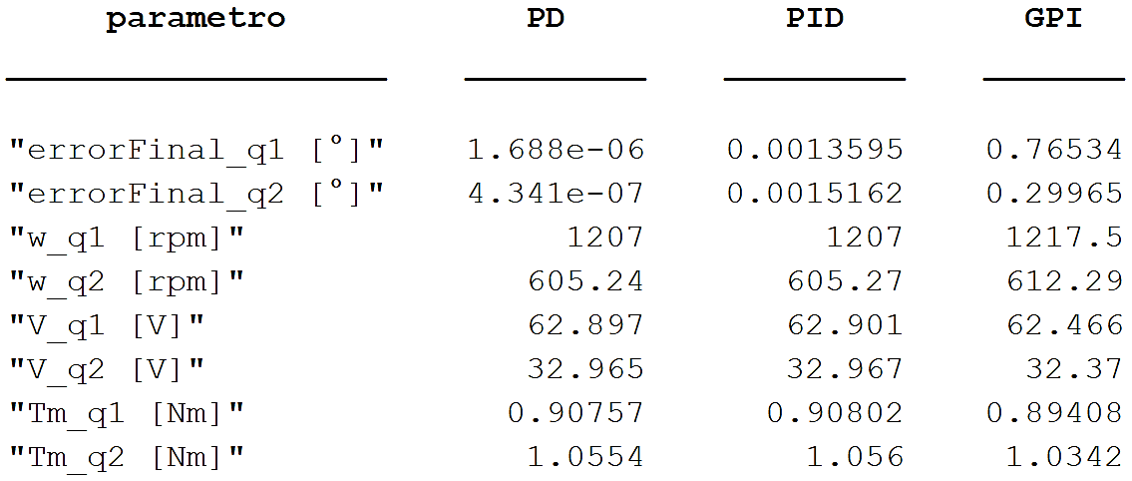
\includegraphics[width=10cm]{imagenes/control15}
    	\caption{Valores obtenidos para el tercer punto de la simulación de los controladores.}
    	\label{fig:control15}
    \end{figure}
    En las Figuras \ref{fig:control16}-\ref{fig:control19} se muestran las gráficas para las posiciones, voltajes de armadura, torques y velocidades angulares, igual que en el primer y segundo punto.
    \begin{figure}[H]
    	\centering
    	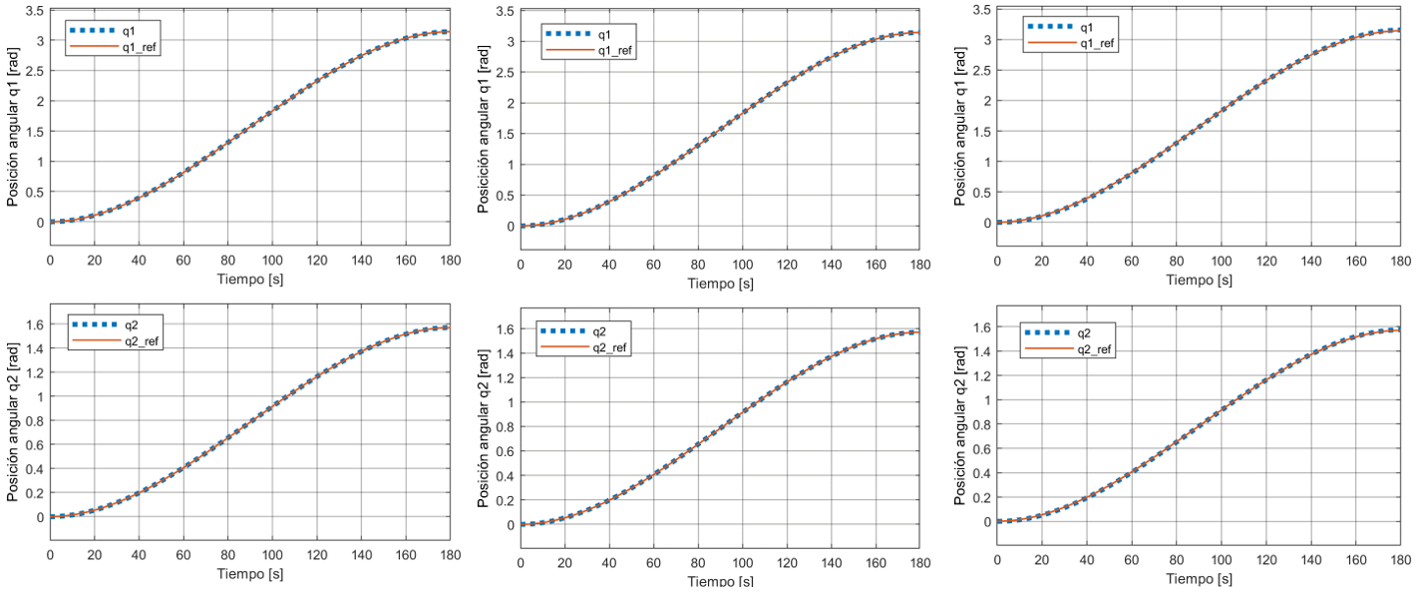
\includegraphics[width=\columnwidth]{imagenes/control16}
    	\caption{Gráficas de las posiciones de referencia y de la junta para el tercer punto.}
    	\label{fig:control16}
    \end{figure}
    \begin{figure}[H]
    	\centering
    	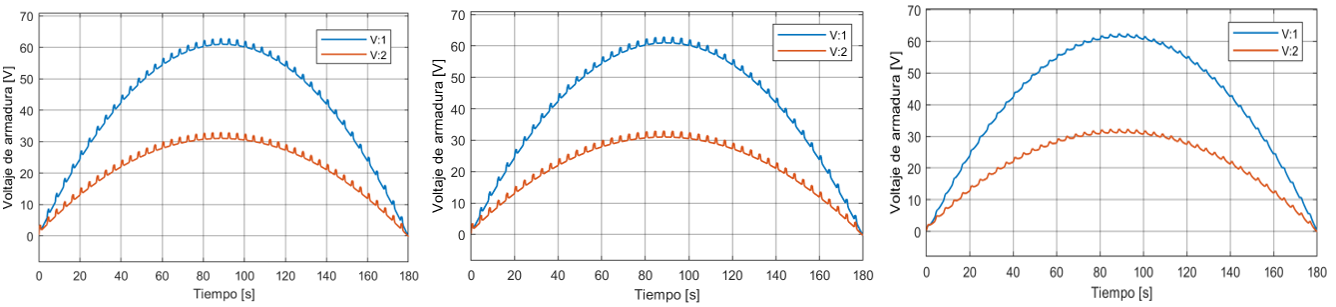
\includegraphics[width=13.5cm]{imagenes/control17}
    	\caption{Gráficas de los voltajes de armadura para el tercer punto.}
    	\label{fig:control17}
    \end{figure}
    \begin{figure}[H]
    	\centering
    	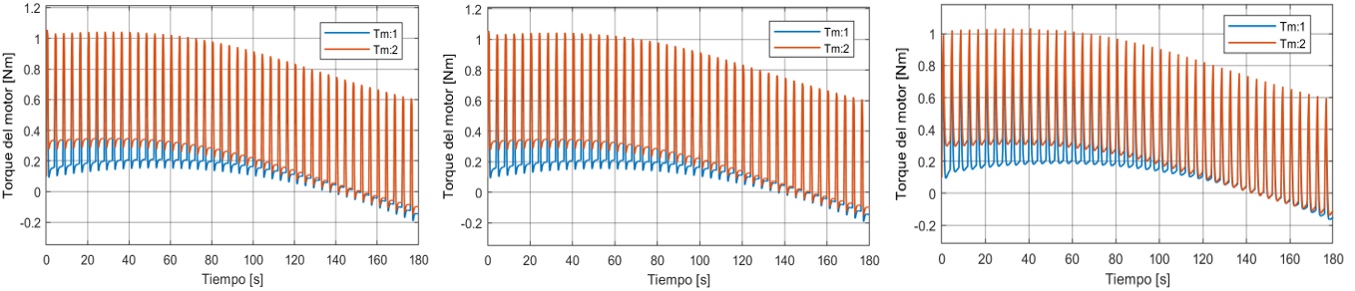
\includegraphics[width=\columnwidth]{imagenes/control18}
    	\caption{Gráficas de los torques demandados para los motores para el tercer punto.}
    	\label{fig:control18}
    \end{figure}
    \begin{figure}[H]
    	\centering
    	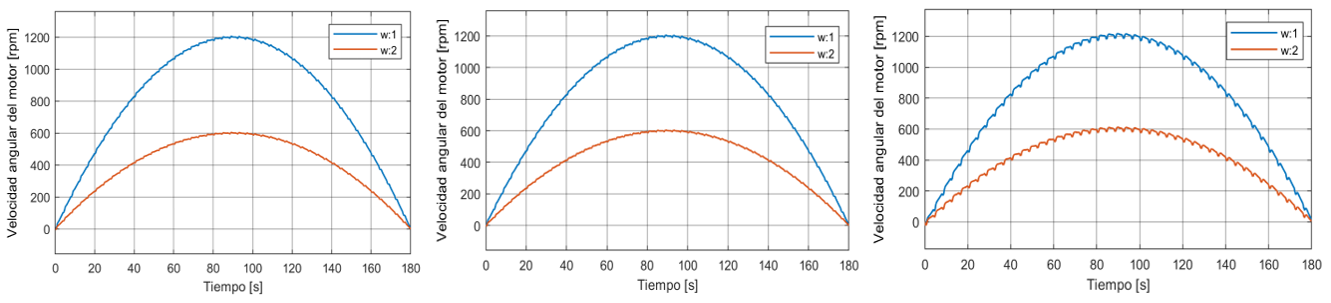
\includegraphics[width=13.5cm]{imagenes/control19}
    	\caption{Gráficas de las velocidades angulares de los motores para el tercer punto.}
    	\label{fig:control19}
    \end{figure}
Al tener un tiempo mayor de respuesta, los 3 controladores poseen casi los mismos valores para el voltaje máximo de armadura y el máximo torque demandado, posiblemente debido al gran tiempo de estabilización. Sin embargo, aún es ligeramente mejor el GPI, a pesar de generar un error mayor que los otros dos controladores, aunque dicho error sigue sin superar 1°.

Después de analizar todos los datos generados por las simulaciones, se optó por seleccionar el controlador GPI como el ganador, debido a su notable reducción en el consumo energético, logrando a la vez un error de seguimiento más que aceptable. A pesar de que los otros dos controladores serían más sencillos y rápidos de implementar, el GPI ofrece un ahorro energético importante para los motores, a cambio de una implementación computacional un poco más compleja. 
\end{itemize}

\newpage
\subsection{Módulo 3: Estructural}

\subsubsection{Cimentación}
Dado que el terreno no colinda con alguna construcción, se considera realizar un cimiento interior. Para un terreno blando se recomienda una zapata con concreto armado. Cuenta con 1.2 m de base y 80 cm de altura, dejando 10 cm de cada lado para polines.

\textbf{\textit{\underline{Cálculo de materiales.}}}

\begin{itemize}
	\item \textbf{\textit{Concreto}} 
	\newline
	Según el Manual de Autoconstrucción\cite{CEMEX}, para obtener una resistencia de 3000 PSI, las medidas de una zapata para un terreno blando son: 1.2 m lado x 1.2 m lado x 0.8 m alto.
	\begin{equation}\label{eq:ec1}
		Volumen = 1.152\;  m^{3}
	\end{equation}
	
	Se considera una relación de mezcla de 1:2:3, en donde: 
	
	% Table generated by Excel2LaTeX from sheet 'Hoja1'
	\begin{table}[H]
		\centering
		%\caption{Add caption}
		\begin{tabular}{|p{4.215em}|p{4.145em}|p{4.285em}|p{4.07em}|}
			\hline
			\multicolumn{1}{|c|}{\textbf{1}} & \multicolumn{1}{c|}{\textbf{2}} & \multicolumn{1}{c|}{\textbf{3}} & \multicolumn{1}{c|}{\textbf{9\%}} \\
			\hline \hline
			Cemento & Arena & Grava & Agua \\
			\hline
			350 kg & $ 0.555 $ $ m^3 $ & $ 0.835 $ $ m^3 $ & $ 0.09 $ $ m^3 $ \\
			\hline
		\end{tabular}%
		%\label{tab:addlabel}%
	\end{table}%
	
	Estas medidas están consideradas por cada $1 \; m^{3}$. Se debe considerar 5\% de cada material de desperdicio.
	
	\textit{Cemento}
	\begin{equation}\label{eq:ec1}
		Cem = \frac{{1.15\;2 m^{3}} \times {350\; kg}}{1\;  m^{3}} = 403.2\; kg + 5\% \;desperdicio = 423.36\; kg  
	\end{equation}

	\textit{Arena}
	\begin{equation}\label{eq:ec1}
		Are = \frac{{1.152\; m^{3}} \times {0.555\; m^{3}}}{1\;  m^{3}} = 0.63936\; m^{3} + 5\%\; desperdicio = 0.671328\;  m^{3}
	\end{equation}

	\textit{Grava}
	\begin{equation}\label{eq:ec1}
		Gra = \frac{{1.152\; m^{3}} \times {0.835\; m^{3}}}{1\;  m^{3}} = 0.96192\; m^{3} + 5\%\; desperdicio = 1.010016\;  m^{3} 
	\end{equation}

	\textit{Agua}
	\begin{equation}\label{eq:ec1}
		Agua = \frac{{0.09\; m^{3}} \times {1.152\; m^{3}}}{1\;  m^{3}} = 0.10368\; m^{3} = 103.68\; L
	\end{equation}
	
\item \textbf{\textit{Mortero}}

Según el Manual de Autoconstrucción \cite{CEMEX}, para obtener una resistencia de 3500 PSI, las medidas de una zapata para un terreno blando son: 1.2m lado x 1.2m lado x 0.1m alto.
\begin{equation}\label{eq:ec1}
	Volumen = 0.144\; m^{3}
\end{equation}

Se considera una relación de mezcla de 1:2, en donde: 

% Table generated by Excel2LaTeX from sheet 'Hoja1'
\begin{table}[H]
	\centering
	%\caption{Add caption}
	\begin{tabular}{|p{4.215em}|p{4.145em}|p{4.07em}|}
		\hline
		\multicolumn{1}{|c|}{\textbf{1}} & \multicolumn{1}{c|}{\textbf{2}} & \multicolumn{1}{c|}{\textbf{9\%}} \\
		\hline
		Cemento & Arena & Agua \\
		\hline
		610 kg & $ 0.97 $ $ m^3 $ & $ 0.09 $ $m^3 $ \\
		\hline
	\end{tabular}%
	%\label{tab:addlabel}%
\end{table}
	Todo esto está considerado por $ m^{3} $, estimando 5\% de cada material de desperdicio.
	
	\textit{Cemento}\\
	\begin{equation}\label{eq:ec1}
		Cem = \frac{{1.144\; m^{3}} \times {610\; kg}}{1\;  m^{3}} = 87.84\; kg + 5\%\; desperdicio = 92.232 \; kg  
	\end{equation}

   \textit{Arena}\\
	\begin{equation}\label{eq:ec1}
		Are = \frac{{1.144 \;m^{3}} \times {0.97\;   m^{3}}}{1\;  m^{3}} = 0. 13968\; m^{3} + 5\%\; desperdicio = 0.146664\;  m^{3} 
	\end{equation}

    \textit{Agua}\\
	\begin{equation}\label{eq:ec1}
		Agua = \frac{{0.09\; m^{3}} \times {1.144\; m^{3}}}{1\;  m^{3}} = 0.01296\; m^{3} = 12.96\; L
	\end{equation}		
%\end{itemize}

\newpage


\item \textbf{\textit{Varilla}}

El manual\cite{CEMEX} menciona el uso de varillas del No. 3 con una separación cada 20 cm colocadas de forma longitudinal y transversal. Se deben usar estribos de 1/4" de grosor. 

\begin{figure}[H]
	\centering
	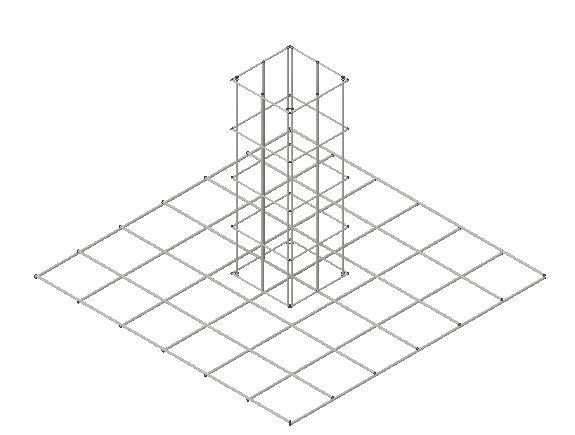
\includegraphics[width=9cm]{imagenes/zapatita.JPG}
	\caption{Parrilla de la zapata}
	\label{fig:zapatita}
\end{figure}

\end{itemize}
%\textit{\textbf{Datos calculados:}}\\
%
%\underline{Factor de carga.}\\
%\begin{center}
%	F.C.=1.4
%\end{center}
%\underline{Esfuerzo máximo de ruptura del concreto:}\\
%\begin{center}
%	F´c = 200 kg/cm$^{2}$
%\end{center}
%\underline{Valor máximo de tensión del acero}:\\
%\begin{center}
%	Fy = 4200 kg/cm$^{2}$
%\end{center}
%\underline{Resistencia del terreno:}\\
%\begin{center}
%	Rt = 21 ton/m$^{2}$
%\end{center}
%\begin{center}
%	Pmax = 6.7 ton
%\end{center}
%\underline{Diámetro del tubo:}\\
%\begin{center}
%	Dt = 8 in = 20.5 cm
%\end{center}
%
%\begin{enumerate}
%	\item \textbf{\textit{Cálculo del área de la zapata.}} \\
%		\begin{equation}\label{eq:ec1}
%		A = \frac{P_{max} + 6\% P_{max}}{Rt} = \frac{6.7 ton + 0.402 ton}{21 ton/m^{2}}
%		\end{equation}
%\end{enumerate}

\subsubsection{Estructura del sistema}
Para contener todos los sistemas y componentes que conforman el seguidor fue necesario diseñar una estructura capaz de soportarlos, así como las cargas producidas por condiciones climáticas como lluvia o golpes de viento y los esfuerzos producidos por el movimiento de todo el seguidor.\\

Del resultado del diseño preliminar final, se decidió dividir la estructura completa en 4 subestructuras (o subconjuntos) relativamente independientes, inicialmente. Esto se ve reflejado en la Figura \ref{fig:descomp}, la cual muestra un diagrama de la primera idea planteada en el diseño preliminar.
\begin{figure}[H]
	\centering
	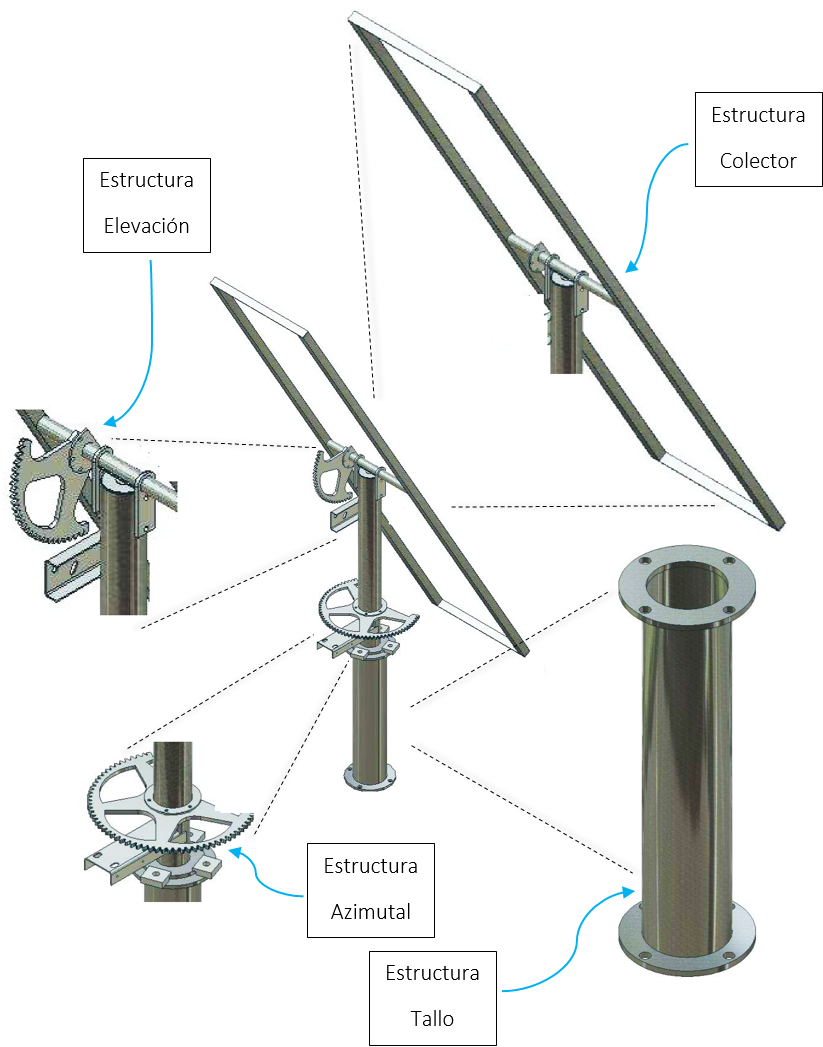
\includegraphics[width=9cm]{imagenes/descomposicion}
	\caption{Descomposición de la estructura del seguidor solar.}
	\label{fig:descomp}
\end{figure}

\textbf{Estructura del Colector}

El diseño de la estructura comenzó por el colector, el cual deberá ser capaz de contener y sujetar los 12 paneles solares. Además, deberá resistir los impactos de viento provenientes de diferentes direcciones. Antes de definir los elementos estructurales se estableció la geometría y disposición del colector, la cual es mostrada en la Figura \ref{fig:colector1}, donde se muestra la vista superior y lateral del colector. El colector estará compuesto por 3 capas: la primera contendrá a los paneles solares, los cuales estarán fijados a soportes distribuidos de forma que permitan la colocación de una matriz de 4x3 paneles, conformando la segunda capa; en la tercera capa se encontrarán los elementos que proporcionarán rigidez a todo el colector, sobre los que descansarán los soportes de la segunda capa.\\

\begin{figure}[H]
	\centering
	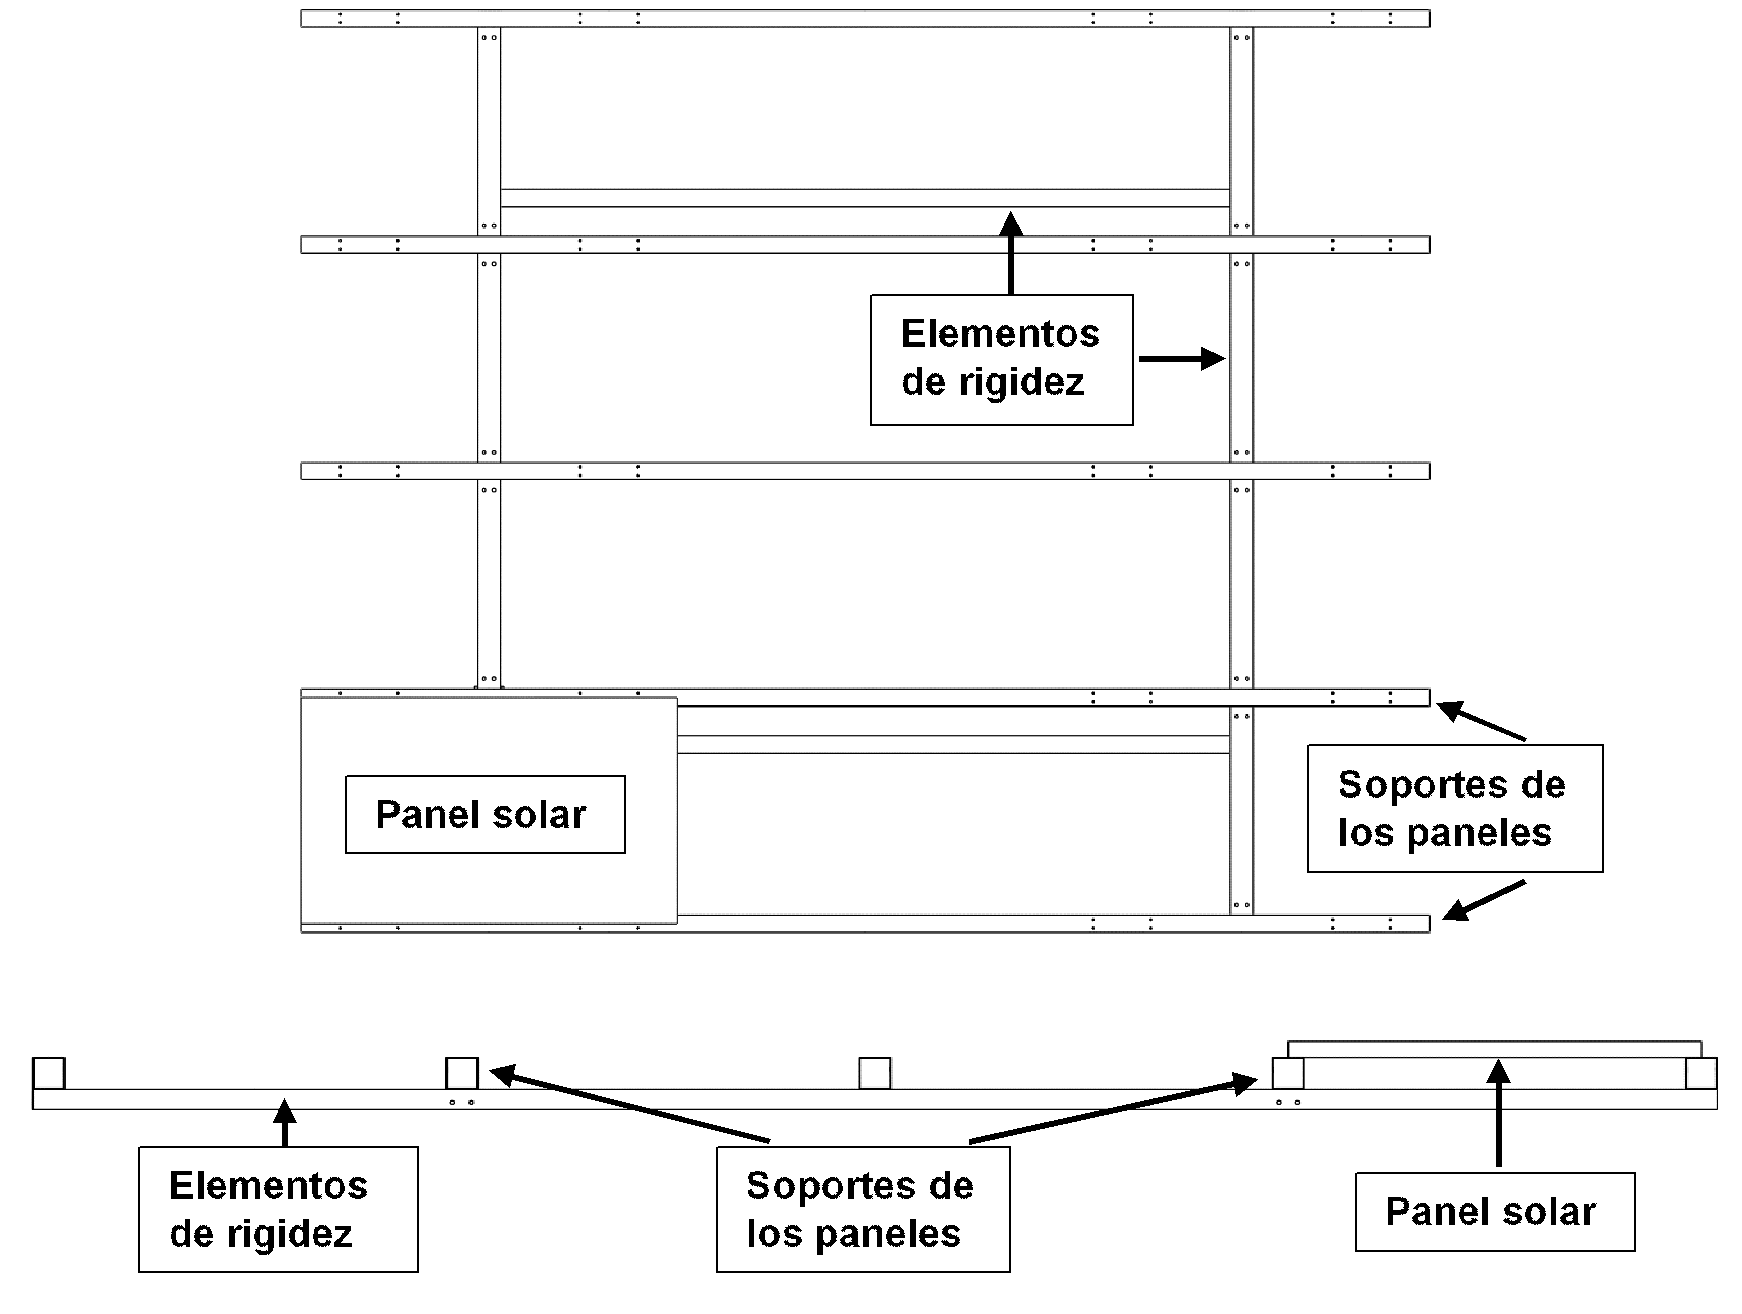
\includegraphics[width=\columnwidth]{imagenes/Esquema_de_la_estructura_del_colector.png}
	\caption{Esquema de la estructura del colector}
	\label{fig:colector1}
\end{figure}

Antes de la selección de los perfiles fue necesario obtener la velocidad del viento de diseño, cuyo valor se obtuvo siguiendo el procedimiento indicado en \cite{DDA9}, sabiendo que la estructura completa posee las siguientes características:

\begin{itemize}
    \item Ninguna de sus dimensiones espaciales es mayor a 20 metros.
	\item Se encuentra en un terreno con varias obstrucciones debidas a los edificios y árboles.
	\item El terreno donde estará el seguidor es plano con inclinaciones prácticamente nulas.
\end{itemize}

Con esta información, el valor de la velocidad de diseño resultó ser de 31.5 m/s (redondeado a 1 décima). Para el cálculo de las cargas principales, se consideraron los planos de ataque del viento principales, los cuales se muestran en la Figura \ref{fig:ataca_viento}.
\begin{figure}[H]
	\centering
	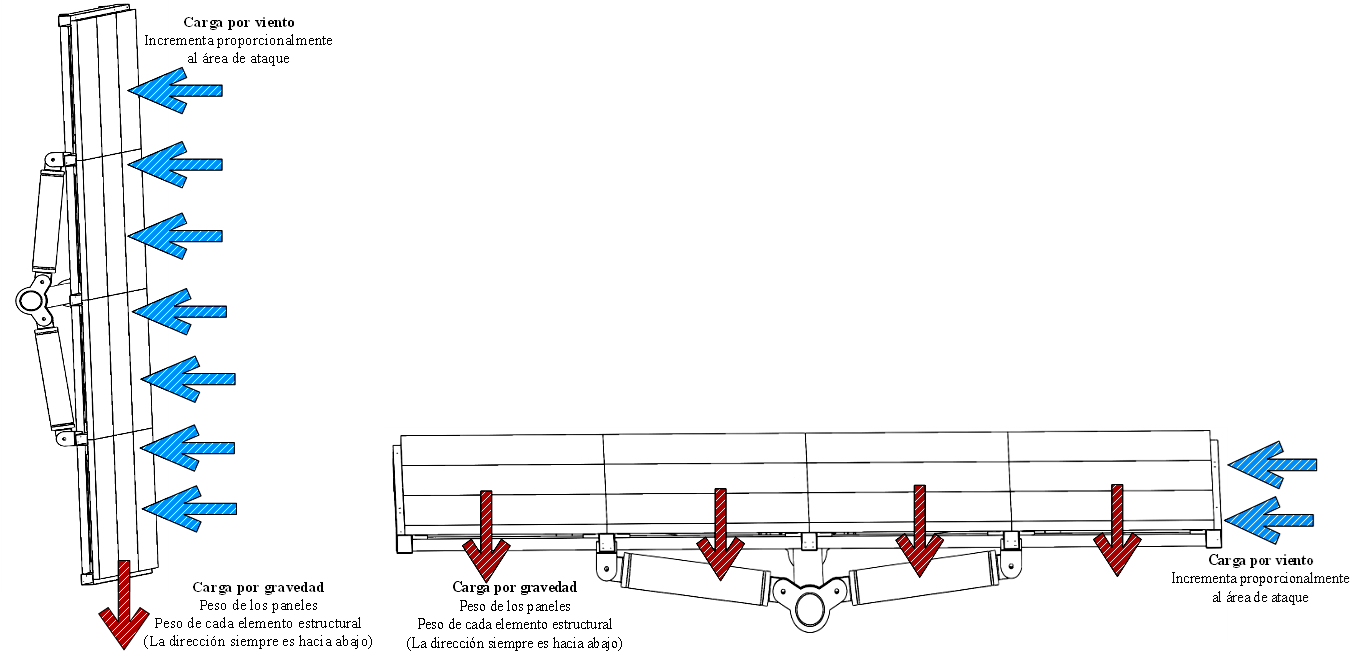
\includegraphics[width=\columnwidth]{imagenes/ataca_viento}
	\caption{Planos de ataque principales del viento: perpendicular a los paneles (izquierda) y paralelo a los paneles (derecha).}
	\label{fig:ataca_viento}
\end{figure}

Posteriormente, se obtuvieron las cargas por viento y por peso. Estos cálculos se muestran en la Tabla \ref{tab:carga_colector}, en la cual el coeficiente de arrastre se obtuvo de tablas en \cite{DDEs4} y \cite{DDEs5}, considerando todo el conjunto de paneles como una sola placa plana perpendicular al viento.
\begin{table}[H]
  \centering
  \caption{Resumen del cálculo de cargas involucradas en el diseño del colector.}
    \begin{tabular}{|p{7cm}|l|}
    \hline
    \textbf{Parámetro} & \textbf{Valor} \\
    \hline \hline
    Velocidad del viento de diseño ($ v_d $) & $ 31.5\ m/s $ \\
    \hline
    Masa de cada panel ($ m_p $) & $ 20\ kg $ \\
    \hline
    Largo x Ancho x Espesor de cada panel & $1.642\ m\ x\ 0.994\    m\ x\ 0.04\ m $ \\
    \hline
    Coeficiente de arrastre ($ c_d $) & $ 2 $ \\
    \hline
    Densidad del aire ($ \rho_a $) & $ 1.22\ kg/m^3 $ \\
    \hline
    Factor de seguridad ($ FS $)  & $ 2 $ \\
    \hline
    Carga por peso: $ F_p= 12 m_p g $ & $ 2355\ N $ \\
    \hline
    Carga por viento (plano perpendicular) \cite{DDEs4} \newline{} $ F_{v1}=\frac{1}{2} c_d \rho_a v_d^2 A_{ef} $ & $ 23710\ N $ \\
    \hline
    Carga por viento (plano paralelo) \cite{DDEs4} \newline{} .$ F_{v1}=  \frac{1}{2} c_d \rho_a v_d^2 A_{ef} $ & $ 2386\ N $ \\
    \hline
    \end{tabular}%
  \label{tab:carga_colector}%
\end{table}%

\newpage
Una vez definidas las cargas y sus direcciones de ataque, se seleccionó el perfil estructural adecuado para manejar estas cargas y que permitiera una fijación sencilla y rápida. Para esto se desarrolló una GUI en MATLAB para mostrar una comparativa entre los materiales a considerar, ingresando los datos necesarios para el análisis de los perfiles estructurales deseados, los cuales fueron considerados como vigas debido a que los perfiles se encuentran cargados y apoyados longitudinalmente, tal y como se muestra en la Figura \ref{fig:viga_sometida}.

\begin{table}[H]
  \centering
  \caption{Expresiones principales del análisis teórico por resistencia para los perfiles estructurales.}
    \begin{tabular}{|c|p{8cm}|}
    \hline
    \multicolumn{1}{|p{5cm}|}{\textbf{Expresión}} & \textbf{Significado} \\
    \hline \hline
    $ R_{i} = \sum _{k=1}^{n}F_{k}*d_{k} $ & Reacción vertical en un apoyo de la viga debida a cargas puntuales \newline{} $ F_k $: Fuerza puntual en la viga \newline{} $ d_k $: Distancia del apoyo a la carga puntual  \newline{} $ n $: Número de cargas puntuales presentes en la viga \\
    \hline
    \multicolumn{1}{|p{5cm}|}{$ M(x) = \sum _{i=1}^{n}P_{i}*(x-d_{i}) $ \newline{} NOTA: Para este trabajo, todas las cargas presentes son: puntuales o linealmente distribuidas.} & Ecuación de momentos en la viga \newline{} También aplica para cargas distribuidas lineales \newline{} $ P_i $: Fuerza puntual o reacción vertical en la viga \newline{} $ d_i $: Distancia del origen a la carga puntual  \newline{} $ m $: Número de cargas puntuales + reacciones presentes en la viga \\
    \hline
    $ M_f=max( M(x) ) $ & Momento flexionante máximo \\
    \hline
    $ \sigma_{ADM}= \frac{R_c}{FS} $ & Esfuerzo normal admisible \newline{} $ R_c $: Resistencia de cedencia del material (también conocida como límite elástico) \\
    \hline
    $ \sigma_f= \frac{M_f*c}{I} $ & Esfuerzo flexionante en vigas \newline{} $ I $: Momento de inercia de la sección transversal del perfil seleccionado \newline{} $ c $: Distancia desde el eje neutro de la sección transversal al punto más alejado de la misma \\
    \hline
    $ \frac{R_c}{FS} = \frac{M_f*c}{I} $ & Relación para obtener la dimensión crítica de la sección transversal del material elegido \\
    \hline
    \end{tabular}%
  \label{tab:expresiones_res}%
\end{table}%

\begin{figure}[H]
	\centering
	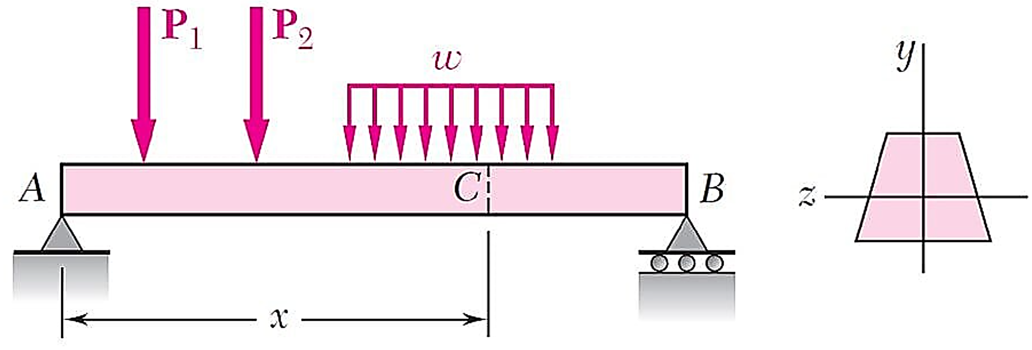
\includegraphics[width=10cm]{imagenes/viga_sometida}
	\caption{Viga sometida a cargas y momentos longitudinales.}
	\label{fig:viga_sometida}
\end{figure}

El análisis realizado por la GUI se basa en la teoría de esfuerzos en vigas de la literatura de resistencia de materiales. La Tabla \ref{tab:expresiones_res} resume las expresiones principales consideradas en el análisis teórico implementado en la GUI.\\

Previo a la programación de la GUI, se realizó una investigación sobre los materiales más comunes utilizados en componentes estructurales. Se llegó a dos tipos de materiales principales: acero, por ser el más utilizado, y aluminio estructural de la serie 6000, por ofrecer prestaciones similares en cuanto a propiedades mecánicas, además de ser mucho más ligero que el acero (aunque un poco más costoso). Para esto, se vio la necesidad de seleccionar al menos un proveedor nacional que contara con estos materiales (principalmente con aluminio estructural). Este proveedor resultó ser la empresa Aluminext, la cual proporciona perfiles estructurales de aluminio 6061, 6063 y 6105 con temples T4, T5 y T6. Las propiedades mecánicas más relevantes de estos aluminios se encuentran en el Anexo 1, obtenidas de la página makeitfrom.com. \\

El funcionamiento de la GUI se basa en dos análisis. El primero permite al usuario seleccionar diferentes materiales, así como ingresar los datos necesarios para definir las cargas presentes en la viga a estudiar (longitudes, masas, factor de seguridad, etc.). Con estos datos, la GUI proporcionará una tabla con los valores de los esfuerzos producidos para cada material seleccionado y su resistencia de cedencia y ruptura. Además, entregará un valor de espesor mínimo para cumplir el factor de seguridad ingresado, espesor que se calculará considerando una sección transversal cuadrada sólida. El segundo análisis permite definir la sección transversal del perfil (restringido a secciones comerciales), establecer su material e ingresar el peso de la viga por metro [kg/m], mientras que el resto de los datos necesarios se toman de los ingresados en el primer análisis; con esto, la GUI generará una tabla con el esfuerzo máximo producido y el factor de seguridad alcanzado con el material y sección seleccionados.\\

Visto de forma más sencilla, el primer análisis es un preliminar para obtener resultados que brinden una referencia para la selección del perfil comercial, el cual será exclusivamente estudiado en el segundo análisis para corroborar que cumpla el factor de seguridad ingresado y soporte los esfuerzos a los que será sometido. La GUI también genera gráficas simples del momento flector máximo para cada tipo de carga (por viento y por peso), permitiendo una mejor comparación entre el peso del material seleccionado y su resistencia.\\

Como evidencia de la funcionalidad de la GUI, se presentan los resultados obtenidos para la selección del perfil correspondiente al soporte de los paneles en la Figuras \ref{fig:GUI_1} y \ref{fig:GUI_2}. Cabe mencionar que las dimensiones ingresadas para la sección transversal en el segundo análisis fueron obtenidas de catálogos de proveedores presentes en México, los cuales son la empresa Aluminext, Aceromex y Acerotienda.

\begin{figure}[H]
	\centering
	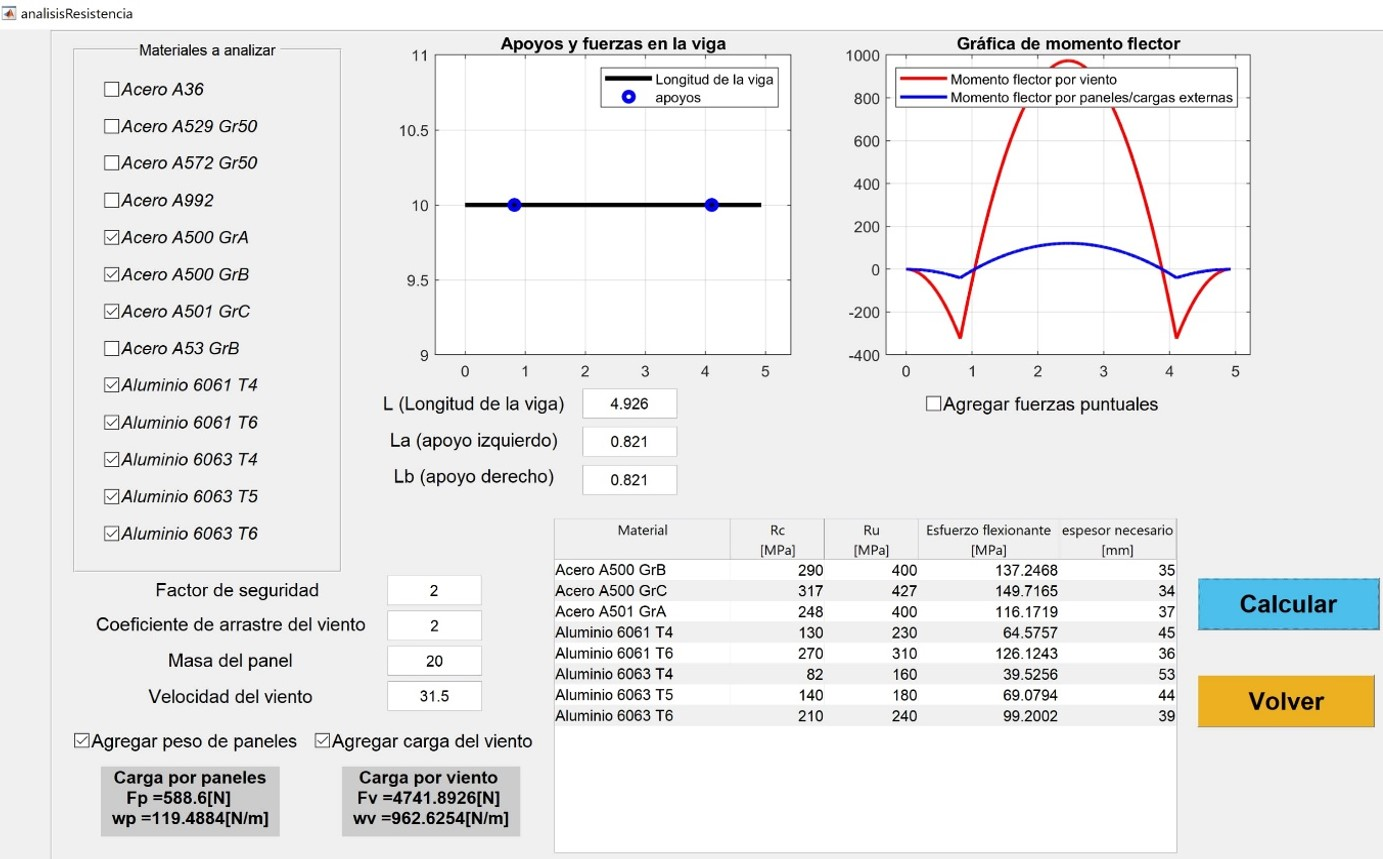
\includegraphics[width=\columnwidth]{imagenes/GUI_1}
	\caption{Primer análisis para el soporte de los paneles.}
	\label{fig:GUI_1}
\end{figure}

\begin{figure}[H]
	\centering
	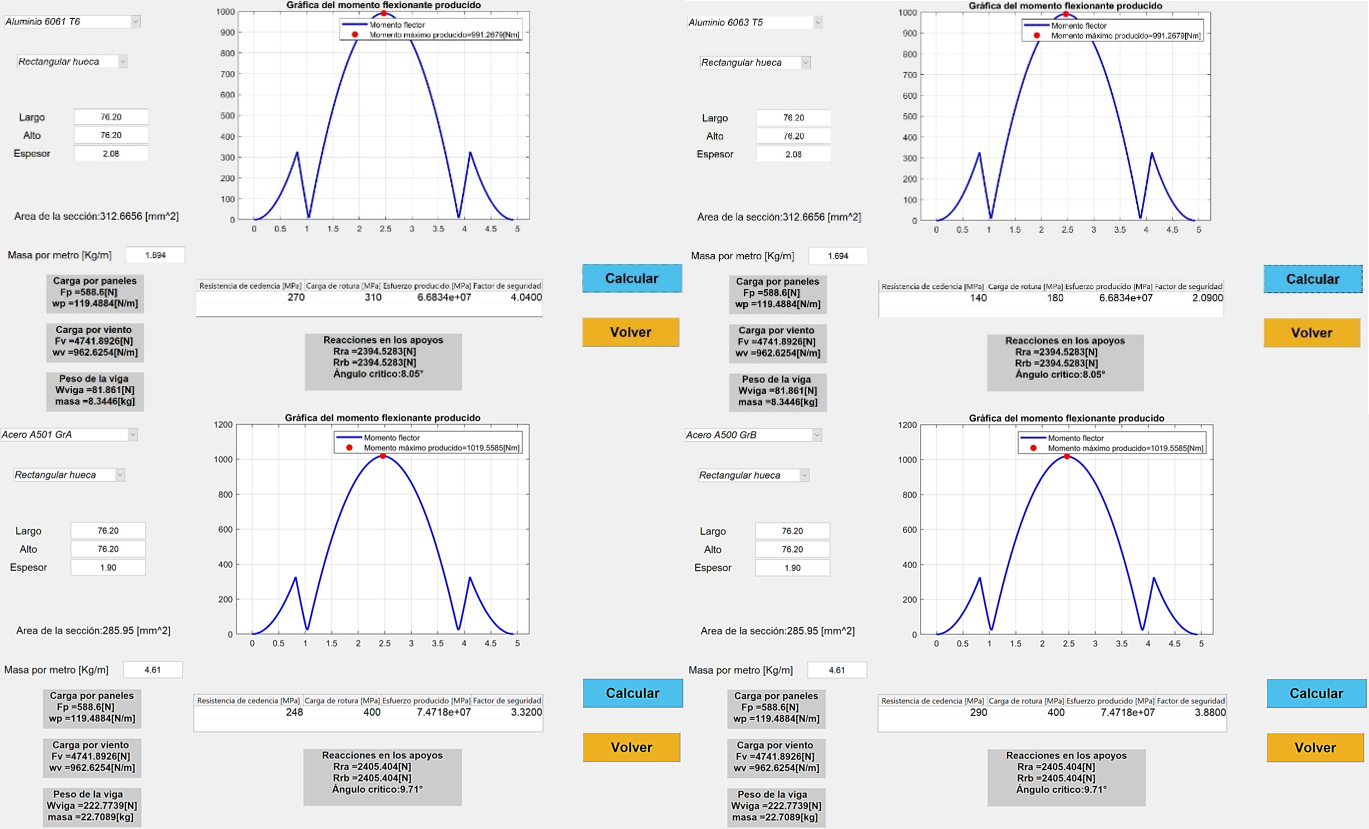
\includegraphics[width=\columnwidth]{imagenes/GUI_2}
	\caption{Resultados obtenidos para un perfil cuadrado con material acero (abajo) y aluminio (arriba).}
	\label{fig:GUI_2}
\end{figure}

Solo se muestran los resultados de los 4 materiales que se consideraron más adecuados en cuanto a una relación entre peso y resistencia. Los demás no cumplían esto ya que, o generaban factores de seguridad muy altos o muy bajos. De los resultados en la figura \ref{fig:GUI_2} se pueden concluir dos cosas: que los aceros poseen una resistencia más alta frente a los aluminios y que, en consecuencia, los aceros son casi el triple de pesados que los aluminios. Debido a esto y al hecho de que los aluminios también cumplen con el factor de seguridad solicitado, a partir de este punto se optó por descartar los aceros para la construcción de la estructura, salvo el soporte principal que corresponde al \textbf{Tallo}.\\

Uno de los objetivos implícitos en este trabajo es conseguir la mejor relación costo-beneficio, por lo que seleccionar un material con un factor de seguridad muy alto tendría un impacto grande en el costo. Es por este motivo que se decidió seleccionar el material \textbf{Aluminio 6063 T5} para el perfil de soporte de paneles, ya que cumple con el factor de seguridad y no lo supera exageradamente.\\

\newpage
Para los elementos de rigidez del colector, se propuso un perfil tipo C (también conocido como canaleta o tipo U), debido a su ligereza y firmeza, cuyos resultados arrojados por el primer análisis de la GUI, los cuales se muestran en la Figura \ref{fig:GUI_3}. Aunque en este primer análisis se consideraron todavía aceros, únicamente fue con el propósito de comparar resultados, para el segundo análisis los aceros fueron descartados completamente, tal y como se mencionó antes.\\

Tomando en cuenta que los resultados de esfuerzos o reacciones en una de las capas del colector influyen en la siguiente capa, así las fuerzas aplicadas sobre el perfil C tienen la misma magnitud que las reacciones calculadas en los perfiles rectangulares.
\begin{figure}[H]
	\centering
	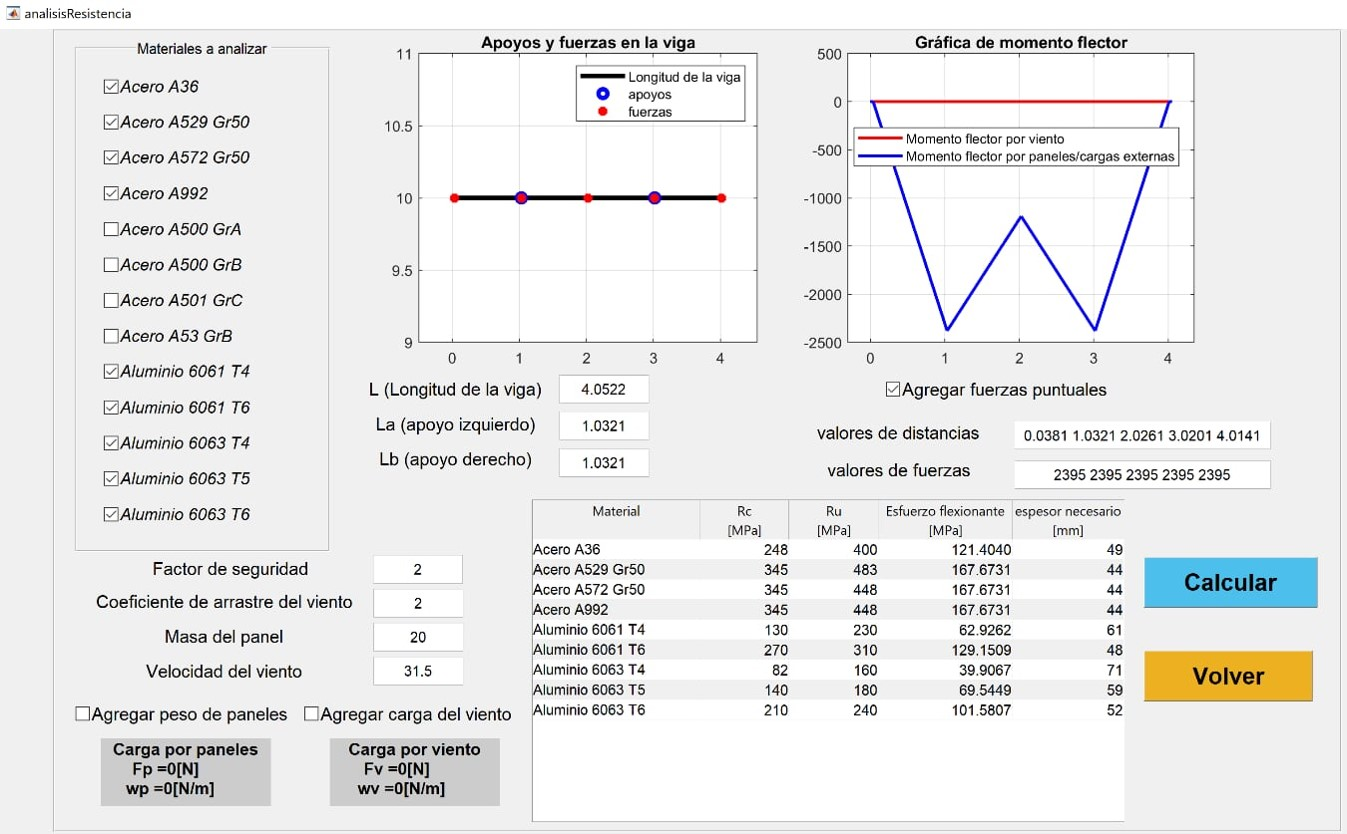
\includegraphics[width=\columnwidth]{imagenes/GUI_3}
	\caption{Primer análisis para el perfil C.}
	\label{fig:GUI_3}
\end{figure}

En la Tabla \ref{tab:perfil_C} se resumen los resultados obtenidos del segundo análisis, considerando las siguientes dimensiones en mm: 101.60 x 50.08 x 5.84.
\begin{table}[H]
  \centering
  \caption{Resultados del segundo análisis teórico para el perfil C.}
    \begin{tabular}{|p{3cm}|r|r|r|r|}
    \hline
    \textbf{Material} & \multicolumn{1}{p{2cm}|}{\textbf{Resistencia de cedencia [MPa]}} & \multicolumn{1}{p{2cm}|}{\textbf{Resistencia de rotura [MPa]}} & \multicolumn{1}{p{2cm}|}{\textbf{Esfuerzo producido [MPa]}} & \multicolumn{1}{p{2cm}|}{\textbf{Factor de seguridad}} \\
    \hline \hline
    Aluminio 6061 T6 & 270 & 310 & 71.284 & 3.79 \\
    \hline
    Aluminio 6063 T6 & 210 & 240 & 71.284 & 2.95 \\
    \hline
    Aluminio 6063 T5 & 140 & 180 & 71.284 & 1.96 \\
    \hline
    \end{tabular}%
  \label{tab:perfil_C}%
\end{table}%

Con estos resultados, la mejor opción es el material \textbf{Aluminio 6063 T6}, ya que cumple con el factor de seguridad sin sobrepasarlo tanto como el 6061 T6.\\

Es importante mencionar que estos resultados y propuestas de perfiles resultaron de varias pruebas y análisis con la GUI y considerando las características mecánicas, facilidades y complejidades que posee cada tipo de perfil. Además, la GUI fue utilizada también para la selección de los perfiles tubulares circulares y ejes, no como criterio determinante, pero si como punto de partida, ya que los detalles de estos componentes se encuentran reportados en sus respectivos módulos (ya sea Azimutal o Elevación).\\

Otra observación es que algunos componentes iniciales fueron modificados debido a los resultados obtenidos en la validación de este módulo, realizada mediante análisis de elemento finito. Uno de estos cambios importantes es el remplazo del perfil C arriba mencionado por un \textbf{perfil cuadrado de 4” x 1/8” de Aluminio 6061 T6}, ya que resultó que, debido a la orientación del perfil, la sección tipo C no era capaz de soportar los esfuerzos ni con el aluminio más resistente.\\

A continuación, se muestran las piezas que conforman la estructura del colector modeladas en el software de diseño SolidWorks. Las Figuras \ref{fig:colec1} y \ref{fig:colec2} corresponden a los perfiles de soporte.
\begin{figure}[H]
	\centering
	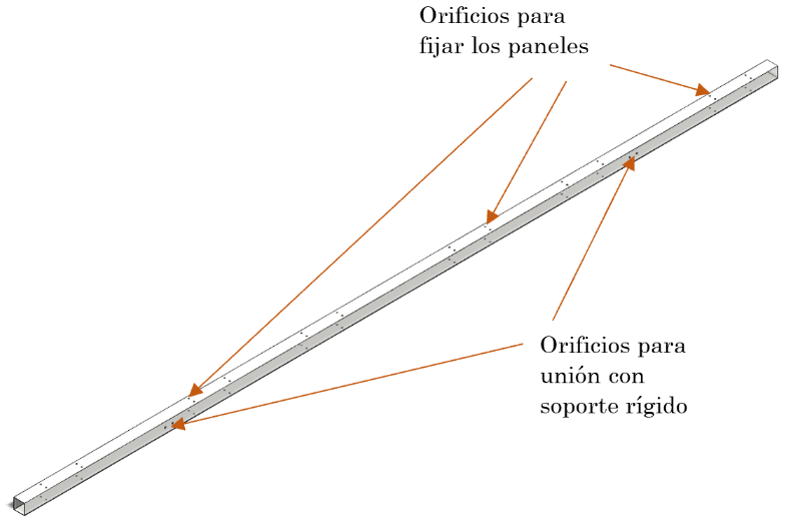
\includegraphics[width=10cm]{imagenes/colec1}
	\caption{Soporte de los paneles solares.}
	\label{fig:colec1}
\end{figure}
\begin{figure}[H]
	\centering
	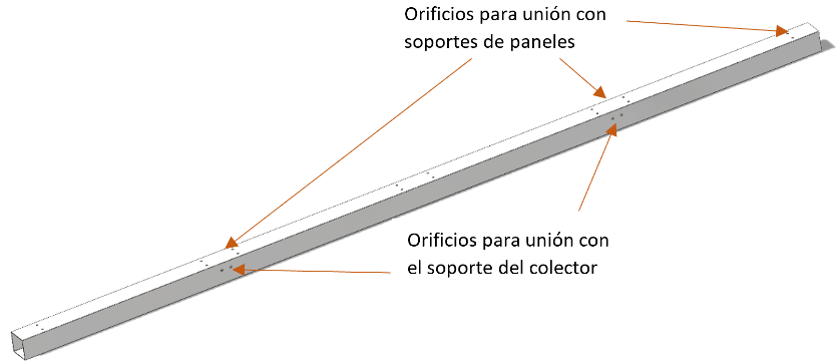
\includegraphics[width=10cm]{imagenes/colec2}
	\caption{Soporte de rigidez de la estructura del colector.}
	\label{fig:colec2}
\end{figure}
\begin{figure}[H]
	\centering
	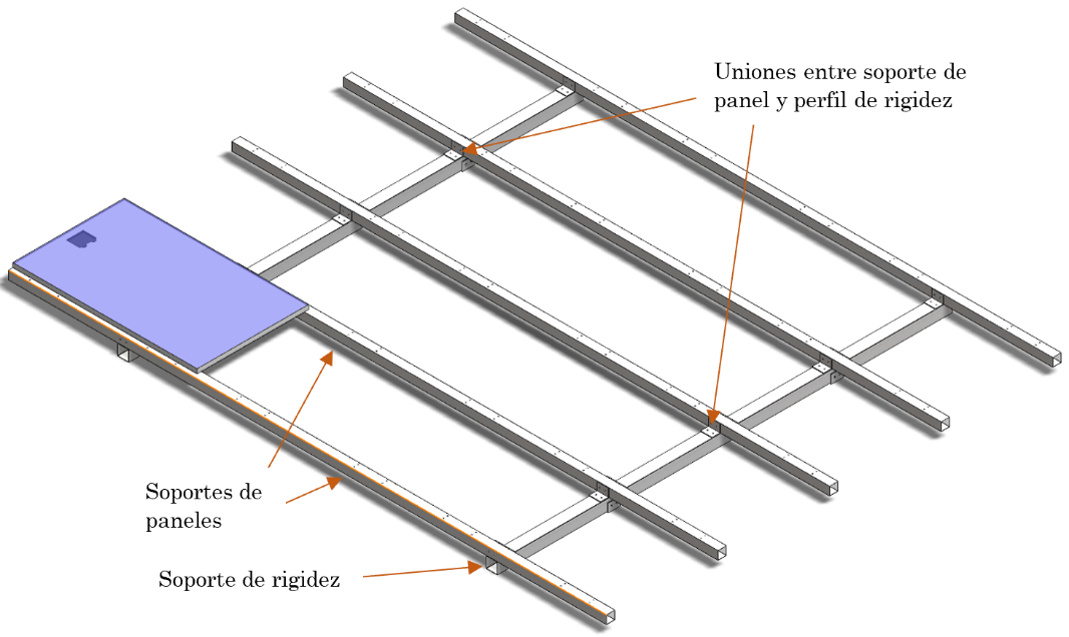
\includegraphics[width=9cm]{imagenes/colec3}
	\caption{Disposición de perfiles y uniones en la estructura del colector.}
	\label{fig:colec3}
\end{figure}

En la Figura \ref{fig:colec3} se muestran las uniones entre los perfiles anteriores y su disposición en el colector. Por otro lado, en la Figura \ref{fig:colec4} se presentan las uniones inferiores entre soportes de rigidez y el soporte principal del colector.

\begin{figure}[H]
	\centering
	\includegraphics[width=12cm]{imagenes/colec4}
	\caption{Uniones inferiores para conexión con el soporte del colector.}
	\label{fig:colec4}
\end{figure}

En la Figura \ref{fig:colec5} se muestra el soporte del colector, el cual está compuesto por dos brazos unidos a un eje principal de movimiento. Este eje es el que permite el movimiento de todo el colector, el cual descansará sobre una plataforma que es descrita en la estructura de elevación. La sección libre de los brazos debería ir soldada a las uniones descritas en la figura anterior, permitiendo así una fijación completa sin perder modularidad en las piezas, ya que dichas uniones van atornilladas a los perfiles de rigidez.

\begin{figure}[H]
	\centering
	\includegraphics[width=13cm]{imagenes/colec5}
	\caption{Soporte principal del colector.}
	\label{fig:colec5}
\end{figure}

Finalmente, en la Figura \ref{fig:colec6} se presenta la estructura del colector. Se puede observar una separación entre columnas de paneles, dicha separación tiene el fin de reducir el impacto del viento y, por lo tanto, el esfuerzo que sufren todos los componentes, siendo de \textbf{20 cm}.

\begin{figure}[H]
	\centering
	\includegraphics[width=\columnwidth]{imagenes/colec6}
	\caption{Estructura del colector ensamblada en SolidWorks.}
	\label{fig:colec6}
\end{figure}

Las dimensiones principales se presentan en la Tabla \ref{tab:colec_medidas}. Para más información y detalles, consultar los planos de las piezas en el Apéndice E.

\begin{table}[H]
  \centering
  \caption{Dimensiones principales de la estructura del colector.}
    \begin{tabular}{|p{8cm}|p{5cm}|}
    \hline
    \textbf{Dimensión} & \textbf{Valor} \\
    \hline \hline
    Longitud soporte paneles & \textit{5.326 [m]} \\
    \hline
    Longitud perfil de rigidez & \textit{4052.2 [m]} \\
    \hline
    Barreno para atornillar paneles & \textit{9 [mm]} \\
    \hline
    Barreno para unión entre soporte de paneles y soporte rígido & \textit{10 [mm]} \\
    \hline
    Barreno para unión con soporte del colector & \textit{12 [mm]} \\
    \hline
    Diámetro del eje del colector & \textit{75 [mm]} \\
    \hline
    Longitud del eje del colector & \textit{3.5 [m]} \\
    \hline
    Barreno de unión entre brazo y eje & \textit{20 [mm]} \\
    \hline
    Dimensiones del colector (Largo x Ancho x Altura) & \textit{5.326 [m] x 4.052.2 [m] x 0.5 [m]} \\
    \hline
    \end{tabular}%
  \label{tab:colec_medidas}%
\end{table}%

\newpage
\textbf{Estructura de Elevación}

Los elementos que conforman este subconjunto no se encontrarán sometidos a cargas importantes, a excepción de la transmisión mecánica, por lo que bastó con seleccionar perfiles que permitieran soportar 100 kg y que fueran sencillos de atornillar, soldar o ensamblar, retomando el uso de únicamente aluminio estructural de la serie 6000. El diseño de la transmisión tipo corona-sinfín aquí mostrada, se explica en el módulo de Elevación, así como la selección de los rodamientos y chumaceras empleados, anillos de retención y chavetas utilizadas.\\

Se comenzó por diseñar una plataforma de tipo reja, con la finalidad de sostener encima de ella todos los elementos que integran la estructura de elevación. Esta plataforma se diseñó con perfil cuadrado, cuya longitud se eligió con base en la longitud del eje del colector, mientras que su ancho fue definido como el menor posible que permitiera contener a los elementos sin ser muy extenso. Esta plataforma se dividió en 3 secciones, dos en los extremos para colocar las chumaceras sobre las que se apoyará el eje de elevación y una central, en la cual se colocarán los elementos mecánicos y eléctricos que permitan generar el movimiento de elevación. La reja de la plataforma se muestra en la Figura \ref{fig:ele1}.

\begin{figure}[H]
	\centering
	\includegraphics[width=13cm]{imagenes/ele1}
	\caption{Reja de la plataforma de elevación.}
	\label{fig:ele1}
\end{figure}

En la sección central se encuentran los elementos más importantes, tales como el motor de movimiento y la transmisión corona-sinfín reductora de velocidad y la chumacera que permite la rotación del tornillo sinfín, todo esto descansando sobre placas de Aluminio 6063 T6 de ½”, tal y como se observa en la Figura \ref{fig:ele2}.

\begin{figure}[H]
	\centering
	\includegraphics[width=9.5cm]{imagenes/ele2}
	\caption{Elementos que integran la sección central de la plataforma de elevación.}
	\label{fig:ele2}
\end{figure}

Dentro del orificio que se aprecia en la corona se colocará el eje del colector, con su respectiva cuña y dos discos que impiden el movimiento axial de la corona, así como con anillos de retención para asegurar que no exista movimiento axial. Por otro lado, el tornillo sinfín se debe conectar al encoder y a la chumacera que le permite rotar, por lo que el encoder deberá ser montado sobre una placa vertical de ¼”. En la Figura \ref{fig:ele3} se muestra un explosionado de los componentes que interactúan con la transmisión corona-sinfín de elevación, donde la cuña se encargará de unir al eje del tornillo sinfín con la caja reductora.

\begin{figure}[H]
	\centering
	\includegraphics[width=9.5cm]{imagenes/ele3}
	\caption{Elementos que interactúan con la transmisión corona-sinfín de elevación.}
	\label{fig:ele3}
\end{figure}

\newpage
Por último, se presenta en la Figura \ref{fig:ele4} la plataforma de elevación con todos sus elementos, en la cual se pueden apreciar las 3 secciones mencionadas anteriormente. Además, se observan las placas de fijación para los sensores de límite de carrera, todas ellas de ¼”. Las placas principales de los extremos sobre las que descansan las chumaceras son de Aluminio 6063 T6 de ½”.

\begin{figure}[H]
	\centering
	\includegraphics[width=\columnwidth]{imagenes/ele4}
	\caption{Estructura de elevación ensamblada en SolidWorks.}
	\label{fig:ele4}
\end{figure}

\textbf{Estructura del Tallo}\\

La mayor parte de las piezas de este subconjunto se describen en el módulo de Azimutal, ya que son componentes mecánicos como rodamientos, ejes o cuñas involucrados directamente en el movimiento azimutal del seguidor solar. El resto de componentes son elementos de fijación, como esquineros, placas de soporte, tornillería y espárragos, salvo el tubo de soporte principal y el acople entre el tallo y la base de elevación. El esqueleto con los elementos de soporte y fijación del tallo se muestra en la Figura \ref{fig:tal1}. Las placas circulares y los esquineros en esta figura están hechos de \textbf{Aluminio 6063 T6}.

\begin{figure}[H]
	\centering
	\includegraphics[width=14cm]{imagenes/tal1}
	\caption{Esqueleto estructural del tallo.}
	\label{fig:tal1}
\end{figure}

\newpage
Los elementos encargados del movimiento azimutal se encuentran en la Figura \ref{fig:tal2}, en la cual se muestra una vista explosionada de todas las piezas no mostradas en la figura anterior.
\begin{figure}[H]
	\centering
	\includegraphics[width=12cm]{imagenes/tal2}
	\caption{Elementos involucrados en el movimiento azimutal (interior).}
	\label{fig:tal2}
\end{figure}

El pasador de fijación permite que el movimiento se transmita a la plataforma de elevación gracias al acople, ya que permite que éste gire junto con el eje del tallo como si fueran uno solo. Las ranuras circulares en el eje son para alojar a los anillos de retención que evitarán el desplazamiento axial de la corona. El conjunto completo del tallo se obtiene combinando las Figuras \ref{fig:tal1} y \ref{fig:tal2}, tal y como se observa en el explosionado de la Figura \ref{fig:tal3}, donde se puede apreciar que no existe interferencia o colisión entre componentes. 
\begin{figure}[H]
	\centering
	\includegraphics[width=11.5cm]{imagenes/tal3}
	\caption{Elementos involucrados en el movimiento azimutal (explosionado).}
	\label{fig:tal3}
\end{figure}

\newpage
Para terminar, en la Figura \ref{fig:ele4} se muestra el Tallo en posición vertical en el seguidor solar, a la izquierda se observa el conjunto interno de piezas ya ensamblado, mientras que a la derecha se observa este mismo conjunto contenido dentro del tubo principal del seguidor.

\begin{figure}[H]
	\centering
	\includegraphics[width=12cm]{imagenes/tal4}
	\caption{Conjunto de piezas internas del tallo.}
	\label{fig:tal4}
\end{figure}

El tubo principal es uno de los elementos estructurales más importantes, ya que brinda un apoyo sobre el centro de masa y aloja el conjunto de piezas que se encarga de ejecutar el movimiento azimutal. Al ser el soporte principal, fue necesario asegurar su resistencia y rigidez ante los esfuerzos por peso y viento (principalmente) y, considerando que ningún elemento va a cargar a este soporte, la posibilidad de utilizar acero para este elemento se hizo presente.\\

De la GUI de MATLAB y la geometría del seguidor se prefirió un perfil circular hueco de más de 4” de diámetro y no más de 3 m de longitud, esto último para evitar mayores esfuerzos por viento y pérdida de estabilidad, además de lo complicado que se vuelve el ensamblaje de la estructura conforme la altura aumenta. Para el análisis teórico de este elemento se elaboró un programa en MATLAB, ya que se presentan esfuerzos combinados, siendo compresión y flexión los que actúan. En la Tabla \ref{tab:esfuerzo_tubo} se muestran las consideraciones tomadas en cuenta para este cálculo.

\begin{table}[H]
  \centering
  \caption{Condiciones consideradas para el diseño del tubo principal.}
    \begin{tabular}{|p{18.355em}|c|}
    \hline
    \textbf{Aspecto} & \textbf{Valor} \\
    \hline \hline
    Factor de seguridad & 2 \\
    \hline
    Carga por flexión* & $ 7904\ N $ \\
    \hline
    Carga por compresión & $ 4905\ N $ \\
    \hline
    Esfuerzo combinado flexión-compresión\newline{} $ W $: Peso soportado.\newline{} $ A_c $: Área de la sección transversal. & $ \sigma= \sigma_f+ \sigma_c= \frac{M_f*c}{I}+\frac{W}{A_c} $ \\
    \hline
    Diámetro exterior comercial obtenido & $ 7.25\ in $ \\
    \hline
    \end{tabular}%
  \label{tab:esfuerzo_tubo}%
\end{table}%
*La carga a soportar por el tubo es 1/3 de la carga de viento total calculada, ya que la estructura contará con dos tubos auxiliares como soportes adicionales.

La salida del programa de MATLAB es la mostrada en la Figura \ref{fig:tal_extra}, donde los últimos dos valores corresponden a la verificación del diámetro obtenido. Se optó por tomar un valor superior al diámetro arrojado por MATLAB, este valor se eligió con base en catálogos y medidas normalizadas, el cual fue de 8” para el diámetro exterior y ¼” de espesor.

\begin{figure}[H]
	\centering
	\includegraphics[width=5.5cm]{imagenes/tal_extra}
	\caption{Cálculo y verificación teóricos del diámetro del tubo de soporte principal.}
	\label{fig:tal_extra}
\end{figure}

% \begin{table}[H]
%   \centering
%   \caption{Cálculo y verificación teóricos del diámetro del tubo de soporte principal.}
%     \begin{tabular}{|l|r|}
%     \hline
%     Diámetro mayor en [cm]: & 18.2627 \\ \hline
%     Diámetro menor en [cm]: & 16.6025 \\ \hline
%     Diámetro mayor comercial en [cm]: & 18.4150 \\ \hline
%     Diámetro mayor comercial en [in]: & 7.2500 \\ \hline
%     Esfuerzo máximo en [MPa]: & 1.2526e+08 \\ \hline
%     Factor de seguridad alcanzado: & 1.9799 \\ \hline
%     \end{tabular}%
%   \label{tab:calcu_tubo}%
% \end{table}%

La carga por compresión se obtuvo de forma aproximada, tomando como referencia la información de propiedades físicas que genera SolidWorks al asignar materiales a las piezas diseñadas. Este cálculo se muestra en la Figura \ref{fig:tal5} para los conjuntos de elevación y colector, valor al cual se le añadieron 20 kg como margen de error y tomando en cuenta la tornillería faltante en el ensamblaje, motivo por el cual se redondeó la masa total soportada a 500 kg.

\begin{figure}[H]
	\centering
	\includegraphics[width=13cm]{imagenes/tal5}
	\caption{Masa aproximada que cargará el tubo principal calculada por SolidWorks.}
	\label{fig:tal5}
\end{figure}

Después de realizar los análisis teóricos y la validación por elemento finito, se determinó que el tubo es capaz de soportar las cargas planteadas, con las siguientes características: \textbf{perfil circular hueco de Acero ASTM A-36 de 8” x ¼”}. El diseño de este tubo en SolidWorks se presenta en la Figura E.

\begin{figure}[H]
	\centering
	\includegraphics[width=3.5cm]{imagenes/tal6}
	\caption{Tubo de acero para el soporte principal del seguidor solar.}
	\label{fig:tal6}
\end{figure}

\textbf{Estructura de Azimutal}

Tal y como sucedió en la estructura de Elevación, los elementos en este subconjunto no están sometidos a cargas de magnitud relevante, a excepción de la transmisión mecánica. En este caso, no resultó viable el armar una plataforma como la de elevación, ya que habría requerido más espacio, provocando colisiones con el colector. Se optó por una plataforma alrededor del tubo de soporte principal, construida a base de \textbf{placa de Aluminio 6063 T6 de ½”}, la cual será sostenida por elementos triangulares, conocidos como nervios, hechos de \textbf{placa de Acero ASM A-36 de ½”}. La razón de haber utilizado acero en vez de aluminio para los nervios es debido a que el tubo principal del seguidor también es de acero, con lo que se planea soldar dichos nervios a ese tubo principal, facilitando la tarea.\\

El esqueleto de la plataforma de azimutal se muestra en las Figuras \ref{fig:azi1} y \ref{fig:azi2}, en las cuales se aprecia el diseño visto desde arriba y visto desde abajo, donde se pueden observar los nervios y sus ranuras de fijación.

\begin{figure}[H]
	\centering
	\includegraphics[width=\columnwidth]{imagenes/azi1}
	\caption{Vista isométrica de la plataforma de azimutal.}
	\label{fig:azi1}
\end{figure}

\begin{figure}[H]
	\centering
	\includegraphics[width=9cm]{imagenes/azi2}
	\caption{Vista inferior de la plataforma de azimutal.}
	\label{fig:azi2}
\end{figure}

Sobre esta plataforma se fijaron todos los componentes que permiten generar el movimiento azimutal del seguidor solar, como el motor eléctrico, la transmisión mecánica, el encoder y la chumacera, por mencionar los más importantes. En la Figura \ref{fig:azi3} se muestra el explosionado de todas las piezas y componentes que se colocan sobre la base de azimutal.

\begin{figure}[H]
	\centering
	\includegraphics[width=11cm]{imagenes/azi3}
	\caption{Vista explosionada de la estructura de azimutal.}
	\label{fig:azi3}
\end{figure}

Vale la pena distinguir algunos elementos dentro de este conjunto. En la Figura \ref{fig:azi4} se presentan estas piezas, donde se observan los soportes para fijar la chumacera y el encoder, minimizando así el juego mecánico entre componentes y, por lo tanto, el error de posición. El tornillo sinfín se conecta con la corona de bronce que forma parte del tallo, gracias a la ranura que posee el tubo principal del tallo.
\begin{figure}[H]
	\centering
	\includegraphics[width=11cm]{imagenes/azi4}
	\caption{Elementos principales involucrados en la transmisión del movimiento azimutal.}
	\label{fig:azi4}
\end{figure}

El diseño de este eje y la selección de encoder y rodamientos se describe a detalle en el módulo azimutal. Finalmente, en la Figura \ref{fig:azi5} se proporciona el conjunto ensamblado de la estructura de azimutal. Todas las placas y perfiles utilizados aquí son de \textbf{Aluminio 6063 T6}, con excepción de los nervios y el tornillo sinfín.

\begin{figure}[H]
	\centering
	\includegraphics[width=10cm]{imagenes/azi5}
	\caption{Estructura de azimutal ensamblada en SolidWorks.}
	\label{fig:azi5}
\end{figure}

\textbf{Estructura de soporte auxiliar}

El diseño de esta estructura inició desde abajo, con el soporte para la pista de movimiento, el cual se encargará de mantener fija esta pista y de soportar 2/3 del peso total de la estructura del seguidor solar. Este soporte está constituido por 6 columnas de \textbf{perfil circular hueco de Aluminio 6063 T5 de 2” x 3/16”}. Ya que estas columnas deberán soportar todo el peso de la estructura, incluyendo los brazos de soporte auxiliares, se decidió agregar 100 kg al valor de masa utilizado para diseñar el tubo de soporte principal, \textbf{resultando para este caso 600 kg de peso total}.

El cálculo teórico de las columnas se realizó utilizando la ecuación del esfuerzo por compresión y asumiendo una sección sólida, tomando como carga de compresión la mitad del valor del peso total, esto para verificar si las columnas son capaces de soportar todo el peso de la estructura.
\begin{equation}
    \sigma_c= \frac{W}{A_c}= \frac{3000\ N}{\frac{\pi}{4}d^2} \rightarrow \frac{R_c}{2}= \frac{12000\ N}{\pi*d^2} \rightarrow d= \sqrt{\frac{24000\ N}{\pi*140\ MPa}} \therefore d \approx 6\ mm
\end{equation}

Con este diámetro, se calculó el área de compresión, para comparar este resultado con el área de contacto que proporciona el perfil de 2” x 3/16”, si el área del perfil es superior al área del diámetro calculado, entonces la columna soportará la compresión.
\begin{equation}
    A_{c1}=\frac{\pi*(6)^2}{4}=28.3\ mm^2
\end{equation}
\begin{equation}
    A_{c2}= \frac{\pi*(50.8^2-41.275^2)}{4}=688.8\ mm^2
\end{equation}

Se puede concluir que el perfil seleccionado es más que adecuado para el esfuerzo que debe soportar, aparentemente. Parecería que está demasiado sobredimensionado el perfil, pero la realidad es que los esfuerzos internos producidos por la flexión de la pista y la deformación producida por el pandeo de la columna hacen que sea necesario considerar un diámetro mucho más grande que el teórico. Esto se justificará en la validación de este componente mediante análisis de elemento finito, en donde los esfuerzos de flexión y deformaciones son tomados en cuenta.

En la Figura \ref{fig:rol1} se muestra el soporte de la pista de movimiento con sus respectivos elementos de unión para fijar y sostener la pista. \textbf{Ambos elementos están hechos de Aluminio 6063 T6}.

\begin{figure}[H]
	\centering
	\includegraphics[width=9cm]{imagenes/rol1}
	\caption{Soporte de la pista de movimiento.}
	\label{fig:rol1}
\end{figure}

Para lograr un movimiento continuo en la pista, se vio la necesidad de seleccionar ruedas capaces de soportar el peso de la estructura y de seguir un movimiento circular sin ocupar un volumen muy grande. Esta rueda fue seleccionada en función de la carga que debe soportar, \textbf{la cual deberá ser de 200 kg} (1/3 del peso total), ya que se utilizará al menos una rueda por cada brazo auxiliar.

El término correcto del componente a seleccionar es rodaja (el conjunto de la rueda con su rodamiento y su soporte de fijación). Esta rodaja se seleccionó del catálogo \cite{DDEs6} del proveedor $ Rodamex $, en su página 65. Esta rodaja es de la línea plana industrial, cuya matrícula es la siguiente: \textbf{H2I101PFGANY}. Sus características se resumen en la Tabla \ref{tab:rodaja}.
\begin{table}[H]
  \centering
  \caption{Características principales de la rodaja seleccionada.}
    \begin{tabular}{|p{11.855em}|p{4.145em}|}
    \hline
    \textbf{Característica} & \textbf{Valor} \\
    \hline \hline
    Diámetro de la rueda & \textit{100 [mm]} \\
    \hline
    Ancho de la rueda (pisada) & \textit{32 [mm]} \\
    \hline
    Altura total & \textit{130 [mm]} \\
    \hline
    Material & \textit{Nylon} \\
    \hline
    Capacidad de carga & \textit{220 [kg]} \\
    \hline
    \end{tabular}%
  \label{tab:rodaja}%
\end{table}%

Se consideró utilizar dos rodajas por brazo para brindar mayor seguridad y para generar un movimiento circular más preciso, colocando las ruedas ligeramente inclinadas sobre una placa de fijación. Esto se puede observar en la Figura \ref{fig:rol2}, mostrando las rodajas que irán debajo de cada brazo auxiliar, unidas mediante una \textbf{placa de Aluminio 6061 T6 de ½”}.
\begin{figure}[H]
	\centering
	\includegraphics[width=10cm]{imagenes/rol2}
	\caption{Conjunto de rodajas con su soporte de fijación.}
	\label{fig:rol2}
\end{figure}

Con base en el ancho de la rueda y el diámetro de la base de elevación, se diseñó la pista de movimiento. Además de esto, fue necesario analizar los esfuerzos presentes en la pista, pero al ser un elemento complejo para analizar de forma teórica, se seleccionó el perfil directamente de los resultados obtenidos por el análisis de elemento finito realizado (ver la sección de validación de este módulo). El perfil que se ajustó a todas estas características resultó ser un \textbf{perfil C de Aluminio 6063 T6 de 3” x 2 13/16” x 7/32”}.

Por otro lado, para el diseño del brazo auxiliar de soporte fue necesario realizar un análisis de esfuerzos combinados, debido a la posición del brazo con respecto a la vertical. En la Figura \ref{fig:rol3} se presenta un diagrama con las dimensiones y fuerzas involucradas en el análisis, donde el valor de L es el máximo considerado.

\begin{figure}[H]
	\centering
	\includegraphics[width=11cm]{imagenes/rol3}
	\caption{Diagrama de fuerzas presentes en el brazo de soporte auxiliar.}
	\label{fig:rol3}
\end{figure}

El análisis de esfuerzos se realizó con ayuda de un programa elaborado en MATLAB, en el cual se programaron las mismas ecuaciones de esfuerzo combinado utilizadas para el diseño del tubo de soporte principal. Con ayuda de este programa se realizaron diversas pruebas para diferentes perfiles redondos comerciales. Como resultado, se llegó a un perfil comercial redondo hueco de Aluminio 6061 T6 de 3 ½” x ¼”. Para este perfil, en la Figura x se muestran los resultados arrojados por el programa para diversos materiales, comprobando que para este material y dimensiones se cumple el factor de seguridad establecido con valor de 2.

\begin{figure}[H]
	\centering
	\includegraphics[width=8cm]{imagenes/rol4}
	\caption{Resultados del análisis teórico para el brazo de soporte auxiliar.}
	\label{fig:rol4}
\end{figure}

En la Figura \ref{fig:rol5} se pueden observar los brazos de soporte auxiliar y los conjuntos de rodajas unidos a los brazos, todo esto apoyado sobre la pista de movimiento sostenida por las 6 columnas anteriormente descritas.

\begin{figure}[H]
	\centering
	\includegraphics[width=10cm]{imagenes/rol5}
	\caption{Vista explosionada de los componentes que integran el soporte auxiliar.}
	\label{fig:rol5}
\end{figure}

\newpage
\textbf{Estructura completa}

Una vez descrito el diseño de cada estructura involucrada en el seguidor solar, se presentan los resultados de todo este módulo. En la Figura \ref{fig:gir1} se observa un explosionado de la estructura completa ensamblada, donde se pueden apreciar todas las subestructuras descritas anteriormente.

\begin{figure}[H]
	\centering
	\includegraphics[width=10cm]{imagenes/gir1}
	\caption{Vista explosionada de la estructura ensamblada del seguidor solar.}
	\label{fig:gir1}
\end{figure}

\newpage
Para terminar, en la Figura \ref{fig:gir4} se muestran dos vistas de la estructura completa ensamblada, en la cual se pueden apreciar los paneles solares colocados y la forma en que el soporte auxiliar sujeta la plataforma de elevación y el colector. Además, estos brazos son lo suficientemente largos como para evitar una colisión entre el extremo del colector y la pista de movimiento.

\begin{figure}[H]
	\centering
	\includegraphics[width=\columnwidth]{imagenes/gir4}
	\caption{Estructura completa del seguidor solar ensamblada en SolidWorks.}
	\label{fig:gir4}
\end{figure}

%REF AGREGADA https://books.google.com.mx/books?hl=es&lr=&id=wgNLDgAAQBAJ&oi=fnd&pg=PT4&dq=ventajas%2Bacero%2B+estructura&ots=YRtD7TX90t&sig=GDm4wSNXcXloZFVLDHnam5I3Njg&redir_esc=y#v=onepage&q=ventajas%2Bacero%2B%20estructura&f=false

%(citar catálogo de Gerdau corsa). 

%https://www.gerdau.com/gerdaucorsa/es/productsservices/products/Document%20Gallery/TABLAS%20DE%20DIMENSIONES_2017.pdf

%------LINKS VENTAJAS
%https://www.asoc-aluminio.es/el-aluminio/ventajas-del-aluminio-en-la-construccion
%https://www.asoc-aluminio.es/el-aluminio/propiedades-del-aluminio
%------lINKS DESVENTAJAS
%https://www.jwwinco.com/es-mx/technical/engineering-tips/pros-and-cons-of-aluminum

% cita de aluminext http://www.aluminext.mx/materiales-equipo/ referencia aluminext

\newpage
\subsubsection{Sensores meteorológicos}
La presión y la temperatura son variables que necesitan ser medidas ya que se requieren en el cálculo de los ángulos de elevación y azimutal del seguidor solar, solicitados por el algoritmo de seguimiento solar. Por otra parte, se requiere conocer la humedad presente en el ambiente del sistema para advertir al mismo de tomar un modo de operación especial para la lluvia o días nublados.\\

\textbf{Sensor de temperatura y humedad}\\

Se realiza la selección de este tipo de sensor, siguiendo las características que se toman como criterios de selección en el árbol de decisiones de la Figura \ref{fig:HT1}:

\begin{figure}[H]
	\centering
	\includegraphics[width=6cm]{imagenes/HT1}
	\caption{Árbol de decisiones para la selección del sensor de Humedad y Temperatura}
	\label{fig:HT1}
\end{figure}

Los 4 sensores restantes corresponden a la siguiente descripción.\\

\underline{\textit{Sensores de humedad y temperatura IP67 serie T9602}}\\

Tomando como criterios la disponibilidad, el precio y la tensión eléctrica con la que se alimentan, resultó seleccionado el siguiente modelo: \underline{\textit{Amphenol T9602-3-D-1}}. \\

Las características eléctricas de este dispositivo se muestran en la Tabla \ref{tabla:caracteristicas} \cite{DDEs1}. \\

\textbf{Sensor de presión}\\
Siguiendo los criterios del árbol de decisiones mostrados en la Figura \ref{fig:P1}, se llegó a 6 sensores candidatos para poder ser utilizados en nuestro sistema. Como criterios de selección finales se tomó en cuenta la disponibilidad del sensor en cuestión, el precio, la exactitud de medición y la alimentación por medio de la herramienta AHP. Así, el sensor seleccionado resultó ser el siguiente: \underline{\textit{PX2EN1XX015PAAAX}}.

\begin{figure}[H]
	\centering
	\includegraphics[width=7cm]{imagenes/P1}
	\caption{Árbol de decisiones para selección del sensor de Presión.}
	\label{fig:P1}
\end{figure}

Las características eléctricas de este dispositivo se muestran en la Tabla \ref{tabla:caracteristicas} de la sección \textbf{Mando Central} \cite{DDEs2}.

\newpage
\subsubsection{Validación (Sistema Estructural)}
Las piezas sometidas a \textbf{cargas mayores a 100 kg o 1000 N} fueron analizadas teóricamente y validadas mediante análisis de elemento finito en SolidWorks 2018. En estas validaciones se analizaron el esfuerzo y deformación producidos en cada pieza, permitiendo así asegurar un factor de seguridad igual o mayor al establecido teóricamente. Estos resultados se muestran para cada pieza analizada, presentando los valores obtenidos para el esfuerzo y deformación máximos y el factor de seguridad con el material aplicado.\\

\textbf{Estructura del colector}\\
Todos los elementos estructurales de este conjunto fueron analizados, ya que se encuentran directamente sometidos a los esfuerzos producidos por el viento y el peso de los paneles solares. Se presenta a continuación la validación por resistencia y rigidez para las 6 piezas más importantes del colector. En la Tabla \ref{tab:val_col1} se resumen las características estructurales más importantes de cada pieza, así como la figura como evidencia del análisis de elemento finito realizado computacionalmente.

\begin{table}[H]
  \centering
  \caption{Características principales de las piezas de la estructura del colector validadas por análisis de elemento finito.}
    \begin{tabular}{|p{1.8cm}|p{9.645em}|p{3.5cm}|c|c|}
    \hline
    \textbf{Pieza} & \textbf{Tipo de perfil y material} & \textbf{Sección transversal [mm]} & \multicolumn{1}{p{3cm}|}{\textbf{Resistencia de cedencia [MPa]}} & \multicolumn{1}{p{1.5cm}|}{\textbf{Figura}} \\
    \hline \hline
    Soporte de paneles & \textit{Perfil Cuadrado\newline{}Aluminio 6063 T5} & \textit{76.2 x 76.2 x 2.08} & \textit{140} & \ref{fig:val_col1} \\
    \hline
    Soporte de rigidez1 & \textit{Perfil C\newline{}Aluminio 6061 T6} & \textit{101.6 x 50.08 x 5.84} & \textit{270} & \ref{fig:val_col2} \\
    \hline
    Soporte de rigidez2 & \textit{Perfil Cuadrado\newline{}Aluminio 6061 T6} & \textit{101.6 x 101.6 x 3.175} & \textit{270} & \ref{fig:val_col3} \\
    \hline
    Brazo del soporte del colector & \textit{Perfil Circular Hueco\newline{}Aluminio 6061 T6} & \textit{101.6 x 5.27} & \textit{270} & \ref{fig:val_col4} \\
    \hline
    Perno de unión & \textit{Hex – Media rosca\newline{}Acero – calidad 8.8} & \textit{M20 x 120} & \textit{640} & \ref{fig:val_col5} \\
    \hline
    Eje del colector & \textit{Perfil Circular Macizo\newline{}Aluminio 6061 T6} & \textit{3500 (longitud) x 75 (diámetro)} & \textit{270} & \ref{fig:val_col6} \\
    \hline
    \end{tabular}%
  \label{tab:val_col1}%
\end{table}%

\begin{figure}[H]
	\centering
	\includegraphics[width=\columnwidth]{imagenes/val_col1}
	\caption{Esfuerzo y deformación en el soporte de paneles.}
	\label{fig:val_col1}
\end{figure}

\begin{figure}[H]
	\centering
	\includegraphics[width=\columnwidth]{imagenes/val_col2}
	\caption{Esfuerzo y deformación en el soporte de rigidez con perfil C.}
	\label{fig:val_col2}
\end{figure}

\begin{figure}[H]
	\centering
	\includegraphics[width=\columnwidth]{imagenes/val_col3}
	\caption{Esfuerzo y deformación en el soporte de rigidez con perfil cuadrado.}
	\label{fig:val_col3}
\end{figure}

\begin{figure}[H]
	\centering
	\includegraphics[width=\columnwidth]{imagenes/val_col4}
	\caption{Esfuerzo y deformación en el brazo del soporte del colector.}
	\label{fig:val_col4}
\end{figure}

\begin{figure}[H]
	\centering
	\includegraphics[width=\columnwidth]{imagenes/val_col5}
	\caption{Esfuerzo y deformación en el perno de unión.}
	\label{fig:val_col5}
\end{figure}

\begin{figure}[H]
	\centering
	\includegraphics[width=\columnwidth]{imagenes/val_col6}
	\caption{Esfuerzo y deformación en el soporte del colector, incluyendo el eje de movimiento.}
	\label{fig:val_col6}
\end{figure}

Para las piezas que no muestran su límite elástico en su respectiva figura, se muestra la comprobación de su factor de seguridad en la Figura \ref{fig:val_col7}, estas piezas son el brazo de soporte del colector, el perno de unión y el eje del colector (en ese orden), validando que todos cumplan un factor de seguridad igual o mayor a 2.

\begin{figure}[H]
	\centering
	\includegraphics[width=11.5cm]{imagenes/val_col7}
	\caption{Validación de factores de seguridad en piezas del colector.}
	\label{fig:val_col7}
\end{figure}

La Tabla \ref{tab:val_col2} resume los resultados presentados en las figuras anteriores, mostrando los valores del esfuerzo, deformación y factor de seguridad obtenidos para cada pieza simulada.

\begin{table}[H]
  \centering
  \caption{Resultados del análisis por elemento finito para las piezas de la estructura del colector.}
    \begin{tabular}{|p{3.5cm}|p{2cm}|c|c|}
    \hline
    \textbf{Pieza} & \textbf{Esfuerzo [MPa]} & \multicolumn{1}{p{2.5cm}|}{\textbf{Deformación [mm]}} & \multicolumn{1}{p{2cm}|}{\textbf{Factor de seguridad}} \\
    \hline \hline
    Soporte de paneles & \textit{+65.76}\newline{}\textit{-65.76} & \textit{26.81} & \textit{2.12} \\
    \hline
    Soporte de rigidez1 & \textit{+151.9}\newline{}\textit{-67.94} & \textit{31.43} & \textit{1.77} \\
    \hline
    Soporte de rigidez2 & \textit{+138}\newline{}\textit{+9.6x10-3} & \textit{3.525} & \textit{1.96} \\
    \hline
    Brazo del soporte del colector & \textit{+140.3}\newline{}\textit{- 4.259x10-3} & \textit{14} & \textit{1.92} \\
    \hline
    Perno de unión & \textit{+250.9} & \textit{0.3758} & \textit{2.6} \\
    \hline
    Soporte del colector* & \textit{+149.6}\newline{}\textit{+23.07x10-3} & \textit{38.41} & \textit{2.96} \\
    \hline
    \end{tabular}%
  \label{tab:val_col2}%
\end{table}%

* El factor de seguridad mostrado aquí es el del eje del colector, validando que los esfuerzos en este eje son menores al esfuerzo máximo en todo el soporte.\\

De la Tabla \ref{tab:val_col2} se puede observar que el soporte de rigidez1 no cumple con el factor de seguridad establecido. En la sección del diseño del módulo estructural se mencionó el cambio de este perfil debido a su incapacidad para soportar los esfuerzos presentes, riesgo que se detectó al realizar un análisis de elemento finito, por lo que fue necesario cambiarlo por otro perfil estructural que sí soportara dichos esfuerzos. Ese perfil es el soporte de rigidez2, el cual apenas cumple el factor de seguridad. Para el resto de las piezas, el factor de seguridad se cumple en un valor aceptable, principalmente el eje del colector, el cual se encuentra sometido a múltiples esfuerzos y es un elemento clave para generar el movimiento de elevación.\\

Las fuerzas utilizadas dentro de cada simulación corresponden a los valores generados por la GUI de MATLAB, tomando en cuenta que el diseño fue descendente, las reacciones generadas en el elemento superior se convierten en las fuerzas que actúan en la siguiente pieza (consultar el diseño del colector). El diseño completo del eje del colector se presenta en el módulo de elevación, donde se muestran las fuerzas y torques a los que se encuentra sometido, así como el proceso de la obtención del diámetro final.\\

\textbf{Estructura de soporte auxiliar}

Ya que este conjunto se encargará de soportar toda la estructura del colector y la plataforma de elevación, estará sometido a una gran carga debida al peso. La altura a la que se encuentran los componentes de esta subestructura es mucho menor que la altura del colector, por lo que los esfuerzos por viento serán mínimos, además de que son elementos delgados, por lo que no poseen mucha área de contacto con el viento.\\

En este conjunto se incluyó el análisis del tubo de soporte principal, para efectos de simplicidad y por ser su función la misma que la del soporte auxiliar: sostener al colector y la plataforma de elevación. En la Tabla \ref{tab:val_rol1} se resumen las características estructurales más importantes de las 5 piezas que conforman esta subestructura. Enseguida, se presentan las validaciones por resistencia y rigidez de cada una de estas piezas.

\begin{table}[H]
  \centering
  \caption{Características principales de las piezas del soporte auxiliar validadas por análisis de elemento finito.}
    \begin{tabular}{|p{6.355em}|p{9.355em}|p{7.355em}|c|p{5.355em}|}
    \hline
    \textbf{Pieza} & \textbf{Tipo de perfil y material} & \textbf{Sección transversal [mm]} & \multicolumn{1}{p{8em}|}{\textbf{Resistencia de cedencia [MPa]}} & \textbf{Figura} \\
    \hline \hline
    Brazo auxiliar de soporte & \textit{Perfil Circular Hueco\newline{}Aluminio 6061 T6} & \textit{88.9 x 6.35} & \textit{270} & \ref{fig:val_rol1} \\
    \hline
    Placa de soporte & \textit{Placa\newline{}Aluminio 6061 T6} & \textit{12.7 (espesor)} & \textit{270} & \ref{fig:val_rol2} \\
    \hline
    Pista de movimiento & \textit{Perfil C\newline{}Aluminio 6063 T6} & \textit{76.2 x 71.88 x 5.08} & \textit{210} & \ref{fig:val_rol3} \\
    \hline
    Columnas de soporte & \textit{Perfil Circular Hueco\newline{}Aluminio 6063 T6} & \textit{50.8 x 4.75} & \textit{210} & \ref{fig:val_rol4} \\
    \hline
    Tubo principal de soporte & \textit{Acero ASTM A-36} & \textit{203.2 x 6.35} & \textit{248} & \ref{fig:val_rol5} \\
    \hline
    \end{tabular}%
  \label{tab:val_rol1}%
\end{table}%

\begin{figure}[H]
	\centering
	\includegraphics[width=11cm]{imagenes/val_rol1}
	\caption{Esfuerzo y deformación en el brazo auxiliar de soporte.}
	\label{fig:val_rol1}
\end{figure}

\begin{figure}[H]
	\centering
	\includegraphics[width=12cm]{imagenes/val_rol2}
	\caption{Esfuerzo y deformación en la placa de soporte.}
	\label{fig:val_rol2}
\end{figure}

\begin{figure}[H]
	\centering
	\includegraphics[width=\columnwidth]{imagenes/val_rol3}
	\caption{Esfuerzo y deformación en la pista de movimiento.}
	\label{fig:val_rol3}
\end{figure}

\begin{figure}[H]
	\centering
	\includegraphics[width=\columnwidth]{imagenes/val_rol4}
	\caption{Esfuerzo y deformación en las columnas de soporte.}
	\label{fig:val_rol4}
\end{figure}
\begin{figure}[H]
	\centering
	\includegraphics[width=11cm]{imagenes/val_rol5}
	\caption{Esfuerzo y deformación en el tubo de soporte principal.}
	\label{fig:val_rol5}
\end{figure}

En la Tabla \ref{tab:val_rol2} se resumen los resultados presentados en las figuras anteriores, donde se muestran los valores del esfuerzo, deformación y factor de seguridad obtenidos para cada una de las piezas simuladas.

\begin{table}[H]
  \centering
  \caption{Resultados del análisis por elemento finito para las piezas estructurales del soporte auxiliar.}
    \begin{tabular}{|p{11.43em}|p{6.5em}|c|c|}
    \hline
    \textbf{Pieza} & \textbf{Esfuerzo [MPa]} & \multicolumn{1}{p{6.145em}|}{\textbf{Deformación [mm]}} & \multicolumn{1}{p{4.93em}|}{\textbf{Factor de seguridad}} \\
    \hline \hline
    Brazo auxiliar de soporte & \textit{83.71\newline{}0.037} & \textit{39.74} & \textit{3.22} \\
    \hline
    Placa de soporte & \textit{122.5\newline{}0.19} & \textit{1.1} & \textit{2.2} \\
    \hline
    Pista de movimiento & \textit{35.53\newline{}0.00715} & \textit{0.07} & \textit{5.91} \\
    \hline
    Columnas de soporte & \textit{20.92\newline{}+ 454.7x10-6} & \textit{0.056} & \textit{10} \\
    \hline
    Tubo principal de soporte & \textit{126.5\newline{}0.9} & \textit{18.83} & \textit{1.96} \\
    \hline
    \end{tabular}%
  \label{tab:val_rol2}%
\end{table}%

Con excepción del tubo principal, se partió de una \textbf{carga total de 600 kg} (información extraída de SolidWorks, la cual ya fue mencionada en el diseño de la estructura del Tallo). Para mayor claridad, se puede consultar el diagrama de fuerzas mostrado en el diseño de la estructura del soporte auxiliar.


%inicio manufactura

%----------------------------------------------------------------:3
%-------------------inicia manufactura
\newpage
\subsubsection{Plan de manufactura}
En este apartado se especifica el desarrollo para obtener las piezas mecánicas del sistema. En la Tabla \ref{tab:MaterialesM} se muestran algunas observaciones acerca de estos en orden de maquinabilidad.

\begin{table}[H]
  \centering
  \caption{Materiales comunes de mecanizar\cite{ProcessP}}
    \begin{tabular}{|p{16.145em}|p{18em}|}
    \hline
    \textbf{Material} & \textbf{Comentarios} \\
    \hline \hline
    Aleaciones de magnesio & Muy fácil de mecanizar, buen acabado superficial, alta vida útil de la herramienta. \\
    \hline
    Aleaciones de aluminio & Muy fácil de mecanizar, aunque las aleaciones de aluminio fundido requieren materiales duros para herramientas. \\
    \hline
    Aleaciones de cobre & Buena maquinabilidad. \\
    \hline
    Hierro fundido gris & Generalmente mecanizable pero abrasivo. \\
    \hline
    Acero carbono & Generalmente mecanizable pero puede tener un acabado superficial pobre. \\
    \hline
    Acero de baja aleación & Generalmente mecanizable. \\
    \hline
    Aceros inoxidables & Ferrítico fácil de mecanizar. \\
    \hline
    Aceros endurecidos / de alta aleación & Endurecedor y abrasivo, puede ser difícil de mecanizar. \\
    \hline
    Superaleaciones a base de níquel & Generalmente difícil de mecanizar, dependiendo del elemento de aleación. \\
    \hline
    Aleaciones de titanio & Difícil de mecanizar, muy abrasivo. \\
    \hline
    \end{tabular}%
  \label{tab:MaterialesM}%
\end{table}%

\textbf{Características de las máquinas a nuestra disposición}

Para los procesos necesarios para cada una de las piezas se considera a la UPIITA-IPN como una alternativa para su elaboración. No se descarta la opción de mandar algunas piezas a un taller especializado. En la Tabla \ref{tab:MaqUPIITA} se registra la maquinaria, cantidades y características con las que cuenta el taller de Máquinas y Herramientas de la UPIITA.

\begin{table}[H]
  \centering
  \caption{Características del Taller de Máquinas y Herramientas de la UPIITA}
    \begin{tabular}{|p{8.645em}|c|p{19.57em}|}
    \hline
    \textbf{Maquinaria} & \textbf{Cantidad} & \textbf{Descripción} \\
    \hline \hline
    Centro de Maquinado Vertical CNC & 1 & Centro de maquinado vertical de 3 ejes con dimensiones de bancada de 762 x 406 x 508 mm, velocidad máxima de trabajo de 8100 rpm y par máximo de 122 Nm a 2000 rpm o 339 Nm a 450 rpm. Cambiador de 24 herramientas y capacidad para 208 L de refrigerante. \\
    \hline
    Dobladora Universal & 1 & Dobladora universal de operación manual para láminas de acero. Dimensiones de 3595 x 840 x 1240 mm con apertura de garganta máxima de 76 mm, capacidad de 3:05 mm y ángulo de 45° de doblez. \\
    \hline
    Guillotina Industrial & 1 & Guillotina industrial de pedal para lámina con dimensiones de trabajo de 1327 mm y capacidad de corte de 1:6 mm en acero suave y 1 mm en acero inoxidable. \\
    \hline
    Esmeril de Banco & 2 & Esmeril de banco de ruedas abrasivas de alimentación monofásica, potencia nominal de 1/4 HP a una velocidad máxima de 3400 rpm. Capacidad de trabajo de 50 minutos por 20 minutos de descanso. \\
    \hline
    Torno Paralelo Universal & 5 & Torno paralelo universal con distancia entre puntos de 1000 mm, bancada de 120 mm de ancho y velocidades de 60 - 2000 rpm. \\
    \hline
    Fresadora Universal & 2 & Fresadora universal con dimensiones de mesa de trabajo de 800 x 230 mm, modo de operación manual y velocidad variable en el rango de las 230 - 1825 rpm. \\
    \hline
    Planta de Soldar & 2 & Planta de soldar para procesos TIG, SMAW y GTAW, con dimensiones de 1085 x 490 x 838 mm y rango de corriente de 5 - 230 A. \\
    \hline
    \end{tabular}%
  \label{tab:MaqUPIITA}%
\end{table}%

\newpage
\textbf{Procesos externos}

Debido a que la escuela no cuenta con una máquina que nos permita rolar o curvear en la Tabla \ref{tab:Rol} se especifican los parámetros necesarios para este proceso. 

\begin{table}[H]
  \centering
  \caption{Parámetros para el proceso de rolado en Aluminio 6063 \cite{Rol}}
    \begin{tabular}{|l|l|}
    \hline
    \textbf{Diámetro interior} & 1423.8 mm \\
    \hline
    \textbf{Diámetro exterior} & 1576.2 mm \\
    \hline
    \textbf{Diámetro medio} & 1500 mm \\
    \hline
    \textbf{Ángulo} & 360° \\
    \hline
    \end{tabular}%
  \label{tab:Rol}%
\end{table}%

\textbf{Relación de piezas}

Teniendo en cuenta la maquinaria con la que se cuenta,  sus características y los procesos externos necesarios para la elaboración de las piezas se presentan en la Tabla \ref{tabla:RelacionPiezaMaq}, donde se especifica la descripción de los procesos, maquinaria y material requerida para la elaboración de cada elemento.

Se implementa un \textit{Código de partes} para identificar de una forma más fácil las piezas del sistema.

\begin{figure}[H]
	\centering
	\includegraphics[width=4cm]{imagenes/nomenclatura}
	\caption{Código de partes}
	\label{fig:nomenclatura}
\end{figure}

\begin{longtable}{@{}|c|r|l|l|c|}
	\caption{Descripción de los procesos involucrados para la manufactura de las piezas}\\
	% aquí añadimos el encabezado de la primera hoja.
	\hline
	\rowcolor[rgb]{ .867,  .922,  .969} \textbf{Componente} & \multicolumn{2}{c|}{\textbf{Descripción de los procesos}} & \textbf{Maquinaria} & \textbf{Material} \\
	\hline \hline
	\endfirsthead
	
	% aquí añadimos el encabezado del resto de hojas.
	\hline
	\rowcolor[rgb]{ .867,  .922,  .969} \textbf{Componente} & \multicolumn{2}{c|}{\textbf{Descripción de los procesos}} & \textbf{Maquinaria} & \textbf{Material} \\
	\hline \hline
	\endhead
	
	% aquí añadimos el fondo de todas las hojas, excepto de la última.
	\multicolumn{6}{c}{}
	\endfoot
	
	% aquí añadimos el fondo de la última hoja.
	\endlastfoot
	
	% aquí añadimos el cuerpo de la tabla.
	CO\_MC1 & 1 & Barrenado & Fresadora universal & Aluminio 6063 T5 \\
    \hline
    CO\_MC2 & 1 & Barrenado & Fresadora universal & Aluminio 6061 T6 \\
    \hline
    \multirow{3}[6]{*}{CO\_MC3} & 1 & Tronzado & Torno universal & \multirow{3}[6]{*}{Aluminio 6061 T6} \\
    \cline{2-4}      & 2 & Ranurado & Fresadora universal &  \\
    \cline{2-4}      & 3 & Barrenado & Fresadora universal &  \\
    \hline
    CO\_MC4 & 1 & Barrenado & Fresadora universal & Aluminio 6063 T5 \\
    \hline
    CO\_ME1 & 1 & Barrenado & Fresadora universal & Aluminio 6063 T5 \\
    \hline
    RO\_MC2 & 1 & Barrenado & Fresadora universal & Aluminio 6063 T6 \\
    \hline
    RO\_MC3 & 1 & Barrenado & Fresadora universal & Aluminio 6061 T6 \\
    \hline
    \multirow{2}[4]{*}{TA\_MC1} & 1 & Ranurado  & Torno universal & \multirow{2}[4]{*}{Aluminio 6063 T6} \\
    \cline{2-4}      & 2 & Barrenado & Fresadora universal &  \\
    \hline
    \multirow{2}[4]{*}{TA\_MC2} & 1 & Ranurado  & Torno universal & \multirow{2}[4]{*}{Aluminio 6063 T6} \\
    \cline{2-4}      & 2 & Barrenado & Fresadora universal &  \\
    \hline
    \multirow{2}[4]{*}{TA\_MC3} & 1 & Ranurado  & Torno universal & \multirow{2}[4]{*}{Aluminio 6063 T6} \\
    \cline{2-4}      & 2 & Barrenado & Fresadora universal &  \\
    \hline
    \multirow{2}[4]{*}{TA\_MC4} & 1 & Ranurado  & Torno universal & \multirow{2}[4]{*}{Aluminio 6063 T6} \\
    \cline{2-4}      & 2 & Barrenado & Fresadora universal &  \\
    \hline
    TA\_MC5 & 1 & Ranurado  & Torno universal & Aluminio 6063 T6 \\
    \hline
    \multirow{5}[10]{*}{TA\_MC6} & 1 & Torneado cónico & Torno universal & \multirow{5}[10]{*}{Aluminio 6063 T6} \\
    \cline{2-4}      & 2 & Cilindrado & Torno universal &  \\
    \cline{2-4}      & 3 & Tronzado & Torno universal &  \\
    \cline{2-4}      & 4 & Ranurado & Fresadora universal &  \\
    \cline{2-4}      & 5 & Barrenado & Fresadora universal &  \\
    \hline
    \multirow{3}[6]{*}{TA\_ME1} & 1 & Cilindrado & Torno universal & \multirow{3}[6]{*}{Aluminio 6063 T6} \\
    \cline{2-4}      & 2 & Ranurado & Torno universal &  \\
    \cline{2-4}      & 3 & Barrenado & Fresadora universal &  \\
    \hline
    AZ\_MC1 & 1 & Barrenado & Fresadora universal & Aluminio 6063 T6 \\
    \hline
    \multirow{2}[6]{*}{AZ\_MC2} & 1 & Ranurado & Torno universal & \multirow{2}[6]{*}{Aluminio 6063 T6} \\
    \cline{2-4}      & 2 & Ranurado & Fresadora universal &  \\
    \hline
    AZ\_MC2      & 3 & Barrenado & Fresadora universal & Aluminio 6063 T6 \\
    \hline
    AZ\_MC3 & 1 & Barrenado & Fresadora universal & Aluminio 6063 T6 \\
    \hline
    AZ\_MC4 & 1 & Barrenado & Fresadora universal & Aluminio 6063 T6 \\
    \hline
    AZ\_MC5 & 1 & Fresado & Fresadora universal & Acero ASTM A-36 \\
    \hline
    AZ\_MC6 & 1 & Fresado & Fresadora universal & Acero ASTM A-36 \\
    \hline
    AZ\_MC7 & 1 & Fresado & Fresadora universal & Acero ASTM A-36 \\
    \hline
    AZ\_MC8 & 1 & Fresado & Fresadora universal & Acero ASTM A-36 \\
    \hline
    AZ\_MC9 & 1 & Barrenado & Fresadora universal & Aluminio 6063 T6 \\
    \hline
    AZ\_MC10 & 1 & Barrenado & Fresadora universal & Aluminio 6063 T6 \\
    \hline
    \multirow{2}[4]{*}{AZ\_MC11} & 1 & Fresado & Fresadora universal & \multirow{2}[4]{*}{Aluminio 6063 T6} \\
    \cline{2-4}      & 2 & Barrenado & Fresadora universal &  \\
    \hline
    \multirow{2}[4]{*}{AZ\_MC12} & 1 & Fresado & Fresadora universal & \multirow{2}[4]{*}{Aluminio 6063 T6} \\
    \cline{2-4}      & 2 & Barrenado & Fresadora universal &  \\
    \hline
    EL\_MC1 & 1 & Barrenado & Fresadora universal & Aluminio 6063 T6 \\
    \hline
    EL\_MC2 & 1 & Barrenado & Fresadora universal & Aluminio 6063 T6 \\
    \hline
    EL\_MC3 & 1 & Barrenado & Fresadora universal & Aluminio 6063 T6 \\
    \hline
    EL\_MC4 & 1 & Barrenado & Fresadora universal & Aluminio 6063 T6 \\
    \hline
    EL\_MC5 & 1 & Barrenado & Fresadora universal & Aluminio 6063 T6 \\
    \hline
    \multirow{2}[4]{*}{EL\_MC6} & 1 & Fresado & Fresadora universal & \multirow{2}[4]{*}{Aluminio 6063 T6} \\
    \cline{2-4}      & 2 & Barrenado & Fresadora universal &  \\
    \hline
    EL\_MC7 & 1 & Barrenado & Fresadora universal & Aluminio 6063 T6 \\
    \hline
    EL\_MC8 & 1 & Barrenado & Fresadora universal & Aluminio 6063 T6 \\
    \hline
    EL\_MC9 & 1 & Barrenado & Fresadora universal & Aluminio 6063 T6 \\
    \hline
    \multirow{2}[4]{*}{EL\_MC10} & 1 & Fresado & Fresadora universal & \multirow{2}[4]{*}{Aluminio 6063 T6} \\
    \cline{2-4}      & 2 & Barrenado & Fresadora universal &  \\
    \hline
    EL\_MC11 & 1 & Barrenado & Fresadora universal & Aluminio 6063 T6 \\
    \hline
    \multirow{2}[4]{*}{EL\_MC12} & 1 & Fresado & Fresadora universal & \multirow{2}[4]{*}{Aluminio 6063 T6} \\
    \cline{2-4}      & 2 & Barrenado & Fresadora universal &  \\
    \hline
    \multirow{2}[4]{*}{EL\_MC13} & 1 & Fresado & Fresadora universal & \multirow{2}[4]{*}{Aluminio 6063 T6} \\
    \cline{2-4}      & 2 & Barrenado & Fresadora universal &  \\
    \hline
    EL\_ME1 & 1 & Cilindrado & Torno universal & Aluminio 6063 T6 \\
    \hline
    EL\_ME1 & 2 & Ranurado & Fresadora universal & Aluminio 6063 T6 \\
    \hline
	% esta línea es importante para que deje un espacio entre la tabla y el nombre de la tabla.
	\label{tabla:RelacionPiezaMaq}
\end{longtable}

\textbf{Hoja de procesos}

Se muestran las hojas de procesos para los elementos estructurales, basadas en \cite{Diego} para la estructura de la tabla. Las velocidades de corte $ V_{c} $ y avance $ f $ se obtienen de \cite{Book} y \cite{ProcessP}. Los cortadores, brocas y buriles se obtienen de los catálogos comerciales \cite{Broca} y \cite{Fresa}.

Los materiales se adquirirán con el corte necesario. Esto debido al costo, explicado en el \textit{Análisis de costos}. Se manufacturará la pieza según los procesos que necesite.

\newpage

%\begin{table}[H]
%  \centering
%  \caption{Hoja de procesos de la pieza CO\_MC1 FAKE}
%    \begin{tabular}{|r|p{10.75em}|p{11em}|p{3em}|p{3.25em}|p{3.5em}|}
%    \hline
%    \multicolumn{2}{|p{12em}|}{\scriptsize Material: Aluminio 6063 T5 \newline{}Tamaño de Perfil: 3" $ x $ 3" $ x $ 5326mm  \newline{}\newline{}Material Herramienta.\newline{}Barrenado: Acero al Carbón HSS\newline{} } & \multicolumn{4}{|p{20.75em}|} {\vspace{0.25mm} \centering  \includegraphics[angle=0,height=6cm]{imagenes/I_CO_MC1}} \\
%    \hline
%   \rowcolor[rgb]{ .886,  .937,  .855}  \scriptsize\centering\textbf{No.} & \scriptsize\centering\textbf{Operación} & \scriptsize\centering\textbf{Herramienta} & \scriptsize\centering\textbf{$ V_{c} $ $ (m/min) $} & \scriptsize\centering\textbf{$ f $ $ (mm/rev) $} & \scriptsize\textbf{ $ a_{p} $  $ (mm) $ } \\
%    \hline
%    \scriptsize 1     & \scriptsize Montaje y alineado de material & \scriptsize -     & \scriptsize {-} & \scriptsize{-} & \scriptsize {-} \\
%    \hline
%    \scriptsize 2     & \scriptsize Barrenado para tornillos & \scriptsize Broca de Zanco Recto 9mm & \scriptsize 118.872 & \scriptsize 787.4 &  \scriptsize {-} \\
%    \hline
%    \scriptsize 3     & \scriptsize Barrenado para tornillos & \scriptsize Broca de Zanco Recto 10mm & \scriptsize 118.872 & \scriptsize 787.4 & \scriptsize {-} \\
%    \hline
%    \scriptsize 4     & \scriptsize Giro de pieza & \scriptsize -     & \scriptsize {-} & \scriptsize {-} & \scriptsize - \\
%    \hline
%    \scriptsize 5     & \scriptsize Barrenado para tornillos & \scriptsize Broca de Zanco Recto 9mm & \scriptsize 118.872 & \scriptsize 787.4 & \scriptsize - \\
%    \hline
%    \scriptsize 6     & \scriptsize Barrenado para tornillos & \scriptsize Broca de Zanco Recto 10mm & \scriptsize 118.872 & \scriptsize 787.4 & \scriptsize - \\
%    \hline
%    \end{tabular}%
%  \label{tab:pez_caballo}%
%\end{table}%

\begin{table}[H]
  \centering
  \caption{Hoja de procesos de la pieza CO\_MC1}
    \begin{tabular}{|r|p{10.75em}|p{11em}|p{3em}|p{3.25em}|p{3.5em}|}
    \hline
    \multicolumn{2}{|p{12em}|}{\scriptsize Material: Aluminio 6063 T5 \newline{}Tamaño de Perfil: 3" $ x $ 3" $ x $ 5326mm  \newline{}\newline{}Material Herramienta.\newline{}Barrenado: Acero al Carbón HSS\newline{} } & \multicolumn{4}{|p{20.75em}|} {\vspace{0.25mm} \centering  \includegraphics[angle=0,height=10cm]{imagenes/I_CO_MC1}} \\
    \hline
   \rowcolor[rgb]{ .886,  .937,  .855}  \scriptsize\centering\textbf{No.} & \scriptsize\centering\textbf{Operación} & \scriptsize\centering\textbf{Herramienta} & \scriptsize\centering\textbf{$ V_{c} $ $ (m/min) $} & \scriptsize\centering\textbf{$ f $ $ (mm/rev) $} & \scriptsize\textbf{ $ a_{p} $  $ (mm) $ } \\
    \hline
    \scriptsize 1     & \scriptsize Montaje y alineado de material & \scriptsize -     & \scriptsize {-} & \scriptsize{-} & \scriptsize {-} \\
    \hline
    \scriptsize 2     & \scriptsize Barrenado para tornillos & \scriptsize Broca de Zanco Recto 9mm & \scriptsize 118.872 & \scriptsize 787.4 &  \scriptsize {-} \\
    \hline
    \scriptsize 3     & \scriptsize Barrenado para tornillos & \scriptsize Broca de Zanco Recto 10mm & \scriptsize 118.872 & \scriptsize 787.4 & \scriptsize {-} \\
    \hline
    \scriptsize 4     & \scriptsize Giro de pieza & \scriptsize -     & \scriptsize {-} & \scriptsize {-} & \scriptsize - \\
    \hline
    \scriptsize 5     & \scriptsize Barrenado para tornillos & \scriptsize Broca de Zanco Recto 9mm & \scriptsize 118.872 & \scriptsize 787.4 & \scriptsize - \\
    \hline
    \scriptsize 6     & \scriptsize Barrenado para tornillos & \scriptsize Broca de Zanco Recto 10mm & \scriptsize 118.872 & \scriptsize 787.4 & \scriptsize - \\
    \hline
    \end{tabular}%
  \label{tab:CO_MC1}%
\end{table}%



\begin{table}[H]
  \centering
  \caption{Hoja de procesos de la pieza CO\_MC2}
    \begin{tabular}{|r|p{10.75em}|p{11em}|p{3em}|p{3.25em}|p{3.5em}|}
    \hline
    \multicolumn{2}{|p{12em}|}{\scriptsize Material: Aluminio 6061 T6\newline{}Tamaño de Perfil: 4" $ x $ 4" $ x $ 4052.2mm   \newline{}\newline{}Material Herramienta.\newline{}Barrenado: Acero al Carbón HSS\newline{}} & \multicolumn{4}{|p{20.75em}|} {\vspace{0.25mm} \centering  \includegraphics[angle=0,width=8cm]{imagenes/I_CO_MC2.pdf}} \\
    \hline
   \rowcolor[rgb]{ .886,  .937,  .855}  \scriptsize\centering\textbf{No.} & \scriptsize\centering\textbf{Operación} & \scriptsize\centering\textbf{Herramienta} & \scriptsize\centering\textbf{$ V_{c} $ $ (m/min) $} & \scriptsize\centering\textbf{$ f $ $ (mm/rev) $} & \scriptsize\textbf{ $ a_{p} $  $ (mm) $ } \\
    \hline
    \scriptsize 1     & \scriptsize Montaje y alineado de material & \scriptsize -     & \scriptsize {-} & \scriptsize{-} & \scriptsize {-} \\
    \hline
    \scriptsize 2     & \scriptsize Barrenado para tornillos & \scriptsize Broca de Zanco Recto 10mm & \scriptsize 118.872 & \scriptsize 787.4 & \scriptsize {-} \\
    \hline
    \scriptsize 3     & \scriptsize Barrenado para tornillos & \scriptsize Broca de Zanco Recto 12mm & \scriptsize 118.872 & \scriptsize 787.4 & \scriptsize {-} \\
    \hline
    \scriptsize 4     & \scriptsize Giro de pieza & \scriptsize -     & \scriptsize {-} & \scriptsize {-} & \scriptsize - \\
    \hline
    \scriptsize 5     & \scriptsize Barrenado para tornillos & \scriptsize Broca de Zanco Recto 10mm & \scriptsize 118.872 & \scriptsize 787.4 & \scriptsize - \\
    \hline
    \scriptsize 6     & \scriptsize Barrenado para tornillos & \scriptsize Broca de Zanco Recto 12mm & \scriptsize 118.872 & \scriptsize 787.4 & \scriptsize - \\
    \hline
    \end{tabular}%
  \label{tab:CO_MC2}%
\end{table}%


\begin{table}[H]
  \centering
  \caption{Hoja de procesos de la pieza CO\_MC3}
    \begin{tabular}{|r|p{10.75em}|p{11em}|p{3em}|p{3.25em}|p{3.5em}|}
    \hline
    \multicolumn{2}{|p{12em}|}{\scriptsize Material: Aluminio 6061 T6\newline{}Tamaño de Redondo: $\varnothing$75mm $ x $ 3484mm
     \newline{}\newline{}Material Herramienta.\newline{}Barrenado: Acero al Carbón HSS\newline{}Fresado: Carburo de Tugsteno\newline{}Torneado: Inserto de Carburo\newline{} } & \multicolumn{4}{|p{20.75em}|} {\vspace{0.25mm} \centering  \includegraphics[angle=0,height=11cm]{imagenes/I_CO_MC3}} \\
    \hline
   \rowcolor[rgb]{ .886,  .937,  .855}  \scriptsize\centering\textbf{No.} & \scriptsize\centering\textbf{Operación} & \scriptsize\centering\textbf{Herramienta} & \scriptsize\centering\textbf{$ V_{c} $ $ (m/min) $} & \scriptsize\centering\textbf{$ f $ $ (mm/rev) $} & \scriptsize\textbf{ $ a_{p} $  $ (mm) $ } \\
    \hline
    \scriptsize 1     & \scriptsize Montaje y alineado de material & \scriptsize -     & \scriptsize {-} & \scriptsize{-} & \scriptsize {-} \\
    \hline
    \scriptsize 2     & \scriptsize Tronzado & \scriptsize Portaherramientas exterior para tronzado con plaquilla de punta GHGL 20-2 & \scriptsize 217.932 & \scriptsize - & \scriptsize 3.8 \\
    \hline
    \scriptsize 3     & \scriptsize Ranurado & \scriptsize Cortador Vertical 3/4" 4F & \scriptsize 188.976 & \scriptsize 0.25-1 & \scriptsize 508 \\
     \hline
    \scriptsize 4     & \scriptsize Montaje y alineado de material & \scriptsize -     & \scriptsize {-} & \scriptsize{-} & \scriptsize {-} \\
    \hline
    \scriptsize 5     & \scriptsize Barrenado para flecha & \scriptsize Broca de Zanco Recto 20mm & \scriptsize 118.872 & \scriptsize 787.4 & \scriptsize - \\
    \hline
    \end{tabular}%
  \label{tab:CO_MC3}%
\end{table}%


 

\begin{table}[H]
  \centering
  \caption{Hoja de procesos de la pieza CO\_MC4}
    \begin{tabular}{|r|p{10.75em}|p{11em}|p{3em}|p{3.25em}|p{3.5em}|}
    \hline
    \multicolumn{2}{|p{12em}|}{\scriptsize Material: Aluminio 6063 T5\newline{}Tamaño de Perfil: 3" $ x $ 3"$ x $ 101.6mm  \newline{}\newline{}Material Herramienta.\newline{}Barrenado: Acero al Carbón HSS\newline{}} & \multicolumn{4}{|p{20.75em}|} {\vspace{0.25mm} \centering  \includegraphics[angle=0,width=6cm]{imagenes/I_CO_MC4.pdf}}\\
    \hline
   \rowcolor[rgb]{ .886,  .937,  .855}  \scriptsize\centering\textbf{No.} & \scriptsize\centering\textbf{Operación} & \scriptsize\centering\textbf{Herramienta} & \scriptsize\centering\textbf{$ V_{c} $ $ (m/min) $} & \scriptsize\centering\textbf{$ f $ $ (mm/rev) $} & \scriptsize\textbf{ $ a_{p} $  $ (mm) $ } \\
    \hline
    \scriptsize 1     & \scriptsize Montaje y alineado de material & \scriptsize -     & \scriptsize {-} & \scriptsize{-} & \scriptsize {-} \\
    \hline
    \scriptsize 2     & \scriptsize Barrenado para tornillos & \scriptsize Broca de Zanco Recto 10mm & \scriptsize 118.872 & \scriptsize 787.4 & \scriptsize {-} \\
    \hline
    \scriptsize 3     & \scriptsize Giro de pieza & \scriptsize -     & \scriptsize {-} & \scriptsize {-} & \scriptsize - \\
    \hline
    \scriptsize 4     & \scriptsize Barrenado para tornillos & \scriptsize Broca de Zanco Recto 10mm & \scriptsize 118.872 & \scriptsize 787.4 & \scriptsize - \\
    \hline
    \end{tabular}%
  \label{tab:CO_MC4}%
\end{table}%

\begin{table}[H]
  \centering
  \caption{Hoja de procesos de la pieza CO\_ME1}
     \begin{tabular}{|r|p{10.75em}|p{11em}|p{3em}|p{3.25em}|p{3.5em}|}
    \hline
    \multicolumn{2}{|p{12em}|}{\scriptsize Material: Aluminio 6063 T5\newline{}Tamaño de Perfil: 4.5" $ x $ 3" $ x $ 110mm  \newline{}\newline{}Material Herramienta.\newline{}Barrenado: Acero al Carbón HSS\newline{} }& \multicolumn{4}{|p{20.75em}|} {\vspace{0.25mm} \centering  \includegraphics[angle=0,height=6cm]{imagenes/I_CO_ME1}} \\
    \hline
    \rowcolor[rgb]{ .886,  .937,  .855}  \scriptsize\centering\textbf{No.} & \scriptsize\centering\textbf{Operación} & \scriptsize\centering\textbf{Herramienta} & \scriptsize\centering\textbf{$ V_{c} $ $ (m/min) $} & \scriptsize\centering\textbf{$ f $ $ (mm/rev) $} & \scriptsize\textbf{ $ a_{p} $  $ (mm) $ } \\
    \hline
    \scriptsize 1     & \scriptsize Montaje y alineado de material & \scriptsize -     & \scriptsize {-} & \scriptsize {-} & \scriptsize - \\
    \hline
    \scriptsize 2     & \scriptsize Barrenado para tornillos & \scriptsize Broca de Zanco Recto 12mm & \scriptsize 118.872 & \scriptsize 787.4 & \scriptsize - \\
    \hline
    \end{tabular}%
  \label{tab:CO_ME1}%
\end{table}%

%---rolado_________________________-
\begin{table}[H]
  \centering
  \caption{Hoja de procesos de la pieza RO\_MC2}
     \begin{tabular}{|r|p{10.75em}|p{11em}|p{3em}|p{3.25em}|p{3.5em}|}
    \hline
    \multicolumn{2}{|p{12em}|}{\scriptsize Material: Aluminio 6063 T6\newline{}Tamaño de Perfil: 50.8mm $ x $ 101.6mm $ x $ 100mm  \newline{}\newline{}Material Herramienta.\newline{}Barrenado: Acero al Carbón HSS\newline{} }& \multicolumn{4}{|p{20.75em}|} {\vspace{0.25mm} \centering  \includegraphics[angle=0,width=6cm]{imagenes/I_RO_MC2.pdf}}\\
    \hline
    \rowcolor[rgb]{ 1,  .949,  .8}  \scriptsize\centering\textbf{No.} & \scriptsize\centering\textbf{Operación} & \scriptsize\centering\textbf{Herramienta} & \scriptsize\centering\textbf{$ V_{c} $ $ (m/min) $} & \scriptsize\centering\textbf{$ f $ $ (mm/rev) $} & \scriptsize\textbf{ $ a_{p} $  $ (mm) $ } \\
    \hline
    \scriptsize 1     & \scriptsize Montaje y alineado de material & \scriptsize -     & \scriptsize {-} & \scriptsize {-} & \scriptsize - \\
    \hline
    \scriptsize 2     & \scriptsize Barrenado para tornillos & \scriptsize Broca de Zanco Recto 10mm & \scriptsize 118.872 & \scriptsize 787.4 & \scriptsize - \\
    \hline
    \end{tabular}%
  \label{tab:RO_MC2}%
\end{table}%

\begin{table}[H]
  \centering
  \caption{Hoja de procesos de la pieza RO\_MC3}
     \begin{tabular}{|r|p{10.75em}|p{11em}|p{3em}|p{3.25em}|p{3.5em}|}
    \hline
    \multicolumn{2}{|p{12em}|}{\scriptsize Material: Aluminio 6061 T6\newline{}Tamaño de Placa: 203.2mm $ x $ 381mm   \newline{}\newline{}Material Herramienta.\newline{}Barrenado: Acero al Carbón HSS\newline{} }& \multicolumn{4}{|p{20.75em}|} {\vspace{0.25mm} \centering  \includegraphics[angle=0,width=8cm]{imagenes/I_RO_MC3.JPG}}\\
    \hline
    \rowcolor[rgb]{ 1,  .949,  .8}  \scriptsize\centering\textbf{No.} & \scriptsize\centering\textbf{Operación} & \scriptsize\centering\textbf{Herramienta} & \scriptsize\centering\textbf{$ V_{c} $ $ (m/min) $} & \scriptsize\centering\textbf{$ f $ $ (mm/rev) $} & \scriptsize\textbf{ $ a_{p} $  $ (mm) $ } \\
    \hline
    \scriptsize 1     & \scriptsize Montaje y alineado de material & \scriptsize -     & \scriptsize {-} & \scriptsize {-} & \scriptsize - \\
    \hline
    \scriptsize 2     & \scriptsize Barrenado para tornillos & \scriptsize Broca de Zanco Recto 8.1mm & \scriptsize 118.872 & \scriptsize 787.4 & \scriptsize - \\
    \hline
    \end{tabular}%
  \label{tab:RO_MC3}%
\end{table}%

%---tallo_________________________-

\begin{table}[H]
  \centering
  \caption{Hoja de procesos de la pieza TA\_MC1}
    \begin{tabular}{|r|p{10.75em}|p{11em}|p{3em}|p{3.25em}|p{3.5em}|}
    \hline
    \multicolumn{2}{|p{12em}|}{\scriptsize Material: Aluminio 6063 T6\newline{}Tamaño de Placa: $\varnothing$ 203.2mm $ x $ 6.35mm
     \newline{}\newline{}Material Herramienta.\newline{}Barrenado: Acero al Carbón HSS\newline{}Torneado: Inserto de Carburo\newline{} } & \multicolumn{4}{|p{20.75em}|} {\vspace{0.25mm} \centering  \includegraphics[angle=0,height=8cm]{imagenes/I_TA_MC1.JPG}}\\
    \hline
   \rowcolor[rgb]{ .988,  .894,  .839}  \scriptsize\centering\textbf{No.} & \scriptsize\centering\textbf{Operación} & \scriptsize\centering\textbf{Herramienta} & \scriptsize\centering\textbf{$ V_{c} $ $ (m/min) $} & \scriptsize\centering\textbf{$ f $ $ (mm/rev) $} & \scriptsize\textbf{ $ a_{p} $  $ (mm) $ } \\
    \hline
    \scriptsize 1     & \scriptsize Montaje y alineado de material & \scriptsize -     & \scriptsize {-} & \scriptsize{-} & \scriptsize {-} \\
    \hline
    \scriptsize 2     & \scriptsize Ranurado Interior & \scriptsize Portaherramientas exterior para ranurado con plaquilla de punta GHGL 20-2 & \scriptsize 217.932 & \scriptsize 711.2 & \scriptsize 85 \\
    \hline
    \scriptsize 3     & \scriptsize Montaje y alineado de material & \scriptsize - & \scriptsize - & \scriptsize - & \scriptsize {-} \\
     \hline
    \scriptsize 4     & \scriptsize Barrenado para flecha & \scriptsize Broca de Zanco Recto 20mm & \scriptsize 118.872 & \scriptsize 787.4 & \scriptsize - \\
    \hline
    \end{tabular}%
  \label{tab:TA_MC1}%
\end{table}%


\begin{table}[H]
  \centering
  \caption{Hoja de procesos de la pieza TA\_MC2}
    \begin{tabular}{|r|p{10.75em}|p{11em}|p{3em}|p{3.25em}|p{3.5em}|}
    \hline
    \multicolumn{2}{|p{12em}|}{\scriptsize Material: Aluminio 6063 T6\newline{}Tamaño de Placa: $\varnothing$ 190.5mm $ x $ 6.35mm
     \newline{}\newline{}Material Herramienta.\newline{}Barrenado: Acero al Carbón HSS\newline{}Torneado: Inserto de Carburo\newline{} } & \multicolumn{4}{|p{20.75em}|} {\vspace{0.25mm} \centering  \includegraphics[angle=0,height=8cm]{imagenes/I_TA_MC2.JPG}}\\
    \hline
   \rowcolor[rgb]{ .988,  .894,  .839}  \scriptsize\centering\textbf{No.} & \scriptsize\centering\textbf{Operación} & \scriptsize\centering\textbf{Herramienta} & \scriptsize\centering\textbf{$ V_{c} $ $ (m/min) $} & \scriptsize\centering\textbf{$ f $ $ (mm/rev) $} & \scriptsize\textbf{ $ a_{p} $  $ (mm) $ } \\
    \hline
    \scriptsize 1     & \scriptsize Montaje y alineado de material & \scriptsize -     & \scriptsize {-} & \scriptsize{-} & \scriptsize {-} \\
    \hline
    \scriptsize 2     & \scriptsize Ranurado Interior & \scriptsize Portaherramientas exterior para ranurado con plaquilla de punta GHGL 20-2 & \scriptsize 217.932 & \scriptsize 711.2 & \scriptsize 68 \\
    \hline
    \scriptsize 3     & \scriptsize Montaje y alineado de material & \scriptsize - & \scriptsize - & \scriptsize - & \scriptsize {-} \\
     \hline
    \scriptsize 4     & \scriptsize Barrenado para flecha & \scriptsize Broca de Zanco Recto 20mm & \scriptsize 118.872 & \scriptsize 787.4 & \scriptsize - \\
    \hline
    \end{tabular}%
  \label{tab:TA_MC2}%
\end{table}%

\begin{table}[H]
  \centering
  \caption{Hoja de procesos de la pieza TA\_MC3}
    \begin{tabular}{|r|p{10.75em}|p{11em}|p{3em}|p{3.25em}|p{3.5em}|}
    \hline
    \multicolumn{2}{|p{12em}|}{\scriptsize Material: Aluminio 6063 T6\newline{}Tamaño de Placa: $\varnothing$ 190.5mm $ x $ 12.7mm
     \newline{}\newline{}Material Herramienta.\newline{}Barrenado: Acero al Carbón HSS\newline{}Torneado: Inserto de Carburo\newline{} } & \multicolumn{4}{|p{20.75em}|} {\vspace{0.25mm} \centering  \includegraphics[angle=0,height=8cm]{imagenes/I_TA_MC3.JPG}}\\
    \hline
   \rowcolor[rgb]{ .988,  .894,  .839}  \scriptsize\centering\textbf{No.} & \scriptsize\centering\textbf{Operación} & \scriptsize\centering\textbf{Herramienta} & \scriptsize\centering\textbf{$ V_{c} $ $ (m/min) $} & \scriptsize\centering\textbf{$ f $ $ (mm/rev) $} & \scriptsize\textbf{ $ a_{p} $  $ (mm) $ } \\
    \hline
    \scriptsize 1     & \scriptsize Montaje y alineado de material & \scriptsize -     & \scriptsize {-} & \scriptsize{-} & \scriptsize {-} \\
    \hline
    \scriptsize 2     & \scriptsize Ranurado Interior & \scriptsize Portaherramientas exterior para ranurado con plaquilla de punta GHGL 20-2 & \scriptsize 217.932 & \scriptsize 711.2 & \scriptsize 45 \\
    \hline
    \scriptsize 3     & \scriptsize Montaje y alineado de material & \scriptsize - & \scriptsize - & \scriptsize - & \scriptsize {-} \\
     \hline
    \scriptsize 4     & \scriptsize Barrenado para flecha & \scriptsize Broca de Zanco Recto 20mm & \scriptsize 118.872 & \scriptsize 787.4 & \scriptsize - \\
    \hline
    \end{tabular}%
  \label{tab:TA_MC3}%
\end{table}%

\begin{table}[H]
  \centering
  \caption{Hoja de procesos de la pieza TA\_MC4}
    \begin{tabular}{|r|p{10.75em}|p{11em}|p{3em}|p{3.25em}|p{3.5em}|}
    \hline
    \multicolumn{2}{|p{12em}|}{\scriptsize Material: Aluminio 6063 T6\newline{}Tamaño de Placa: $\varnothing$ 203.2mm $ x $ 12.7mm
     \newline{}\newline{}Material Herramienta.\newline{}Barrenado: Acero al Carbón HSS\newline{}Torneado: Inserto de Carburo\newline{} } & \multicolumn{4}{|p{20.75em}|} {\vspace{0.25mm} \centering  \includegraphics[angle=0,height=8cm]{imagenes/I_TA_MC4.JPG}}\\
    \hline
   \rowcolor[rgb]{ .988,  .894,  .839}  \scriptsize\centering\textbf{No.} & \scriptsize\centering\textbf{Operación} & \scriptsize\centering\textbf{Herramienta} & \scriptsize\centering\textbf{$ V_{c} $ $ (m/min) $} & \scriptsize\centering\textbf{$ f $ $ (mm/rev) $} & \scriptsize\textbf{ $ a_{p} $  $ (mm) $ } \\
    \hline
    \scriptsize 1     & \scriptsize Montaje y alineado de material & \scriptsize -     & \scriptsize {-} & \scriptsize{-} & \scriptsize {-} \\
    \hline
    \scriptsize 2     & \scriptsize Ranurado Interior & \scriptsize Portaherramientas exterior para ranurado con plaquilla de punta GHGL 20-2 & \scriptsize 217.932 & \scriptsize 711.2 & \scriptsize 60 \\
    \hline
    \scriptsize 3     & \scriptsize Montaje y alineado de material & \scriptsize - & \scriptsize - & \scriptsize - & \scriptsize {-} \\
     \hline
    \scriptsize 4     & \scriptsize Barrenado para flecha & \scriptsize Broca de Zanco Recto 20mm & \scriptsize 118.872 & \scriptsize 787.4 & \scriptsize - \\
    \hline
    \end{tabular}%
  \label{tab:TA_MC4}%
\end{table}%

\begin{table}[H]
  \centering
  \caption{Hoja de procesos de la pieza TA\_MC5}
    \begin{tabular}{|r|p{10.75em}|p{11em}|p{3em}|p{3.25em}|p{3.5em}|}
    \hline
    \multicolumn{2}{|p{12em}|}{\scriptsize Material: Aluminio 6063 T6\newline{}Tamaño de Perfil:   50.8mm  $ x $  50.8mm  $x$  50.8mm 
     \newline{}\newline{}Material Herramienta.\newline{}Barrenado: Acero al Carbón HSS\newline } &  \multicolumn{4}{|p{20.75em}|} {\vspace{0.25mm} \centering  \includegraphics[angle=0,height=8cm]{imagenes/I_TA_MC5.JPG}}\\
    \hline
   \rowcolor[rgb]{ .988,  .894,  .839}  \scriptsize\centering\textbf{No.} & \scriptsize\centering\textbf{Operación} & \scriptsize\centering\textbf{Herramienta} & \scriptsize\centering\textbf{$ V_{c} $ $ (m/min) $} & \scriptsize\centering\textbf{$ f $ $ (mm/rev) $} & \scriptsize\textbf{ $ a_{p} $  $ (mm) $ } \\
    \hline
    \scriptsize 1     & \scriptsize Montaje y alineado de material & \scriptsize -     & \scriptsize {-} & \scriptsize{-} & \scriptsize {-} \\
    \hline
    \scriptsize 2     & \scriptsize Barrenado de tornillos & \scriptsize Broca de Zanco Recto 8mm & \scriptsize 118.872 & \scriptsize 787.4 & \scriptsize - \\
    \hline
    \scriptsize 3     & \scriptsize Giro de pieza & \scriptsize - & \scriptsize - & \scriptsize - & \scriptsize {-} \\
     \hline
     \scriptsize 4    & \scriptsize Barrenado de tornillos & \scriptsize Broca de Zanco Recto 8mm & \scriptsize 118.872 & \scriptsize 787.4 & \scriptsize - \\
    \hline
    \end{tabular}%
  \label{tab:TA_MC5}%
\end{table}%

\begin{table}[H]
  \centering
  \caption{Hoja de procesos de la pieza TA\_MC6}
    \begin{tabular}{|r|p{10.75em}|p{11em}|p{3em}|p{3.25em}|p{3.5em}|}
    \hline
    \multicolumn{2}{|p{12em}|}{\scriptsize Material: Aluminio 6063 T6\newline{}Tamaño de Redondo: $\varnothing$2" $ x $ 304.8mm
     \newline{}\newline{}Material Herramienta.\newline{}Barrenado: Acero al Carbón HSS\newline{}Fresado: Carburo de Tugsteno\newline{}Torneado: Inserto de Carburo\newline{} } & \multicolumn{4}{|p{20.75em}|} {\vspace{0.25mm} \centering  \includegraphics[angle=0,height=8cm]{imagenes/I_TA_MC6.JPG}}\\
    \hline
   \rowcolor[rgb]{ .988,  .894,  .839} \scriptsize\centering\textbf{No.} & \scriptsize\centering\textbf{Operación} & \scriptsize\centering\textbf{Herramienta} & \scriptsize\centering\textbf{$ V_{c} $ $ (m/min) $} & \scriptsize\centering\textbf{$ f $ $ (mm/rev) $} & \scriptsize\textbf{ $ a_{p} $  $ (mm) $ } \\
    \hline
    \scriptsize 1     & \scriptsize Montaje y alineado de material & \scriptsize -     & \scriptsize {-} & \scriptsize{-} & \scriptsize {-} \\
    \hline
    \scriptsize 2     & \scriptsize Torneado Cónico & \scriptsize Buril 1/2" & \scriptsize 217.932 & \scriptsize 711.2 & \scriptsize 5.8 \\
    \hline
    \scriptsize 3     & \scriptsize Cilindrado & \scriptsize Buril 1/2" & \scriptsize 217.932 & \scriptsize 711.2 & \scriptsize 5.7 \\
     \hline
     \scriptsize 4     & \scriptsize Tronzado & \scriptsize Portaherramientas exterior para tronzado con plaquilla de punta GHGL 20-2 & \scriptsize 217.932 & \scriptsize - & \scriptsize 2.9 \\
     \hline
    \scriptsize 5     & \scriptsize Montaje y alineado de material & \scriptsize -     & \scriptsize {-} & \scriptsize{-} & \scriptsize - \\
    \hline
     \scriptsize 6     & \scriptsize Ranurado & \scriptsize Cortador Vertical 3/4" 4F & \scriptsize 188.976 & \scriptsize 0.25-1 & \scriptsize 44.45 \\
    \hline
    \scriptsize 7     & \scriptsize Barrenado para flecha & \scriptsize Broca de Zanco Recto 20mm & \scriptsize 118.872 & \scriptsize 787.4 & \scriptsize - \\
    \hline
    \end{tabular}%
  \label{tab:TA_MC6}%
\end{table}%

\begin{table}[H]
  \centering
  \caption{Hoja de procesos de la pieza TA\_ME1}
    \begin{tabular}{|r|p{10.75em}|p{11em}|p{3em}|p{3.25em}|p{3.5em}|}
    \hline
    \multicolumn{2}{|p{12em}|}{\scriptsize Material: Aluminio 6063 T6\newline{}Tamaño de Redondo: $\varnothing$203.2mm $ x $ 80.5mm
     \newline{}\newline{}Material Herramienta.\newline{}Barrenado: Acero al Carbón HSS\newline{}Torneado: Inserto de Carburo\newline{} } & \multicolumn{4}{|p{20.75em}|} {\vspace{0.25mm} \centering  \includegraphics[angle=0,height=8cm]{imagenes/I_TA_ME1.JPG}}\\
    \hline
   \rowcolor[rgb]{ .988,  .894,  .839} \scriptsize\centering\textbf{No.} & \scriptsize\centering\textbf{Operación} & \scriptsize\centering\textbf{Herramienta} & \scriptsize\centering\textbf{$ V_{c} $ $ (m/min) $} & \scriptsize\centering\textbf{$ f $ $ (mm/rev) $} & \scriptsize\textbf{ $ a_{p} $  $ (mm) $ } \\
    \hline
    \scriptsize 1     & \scriptsize Montaje y alineado de material & \scriptsize -     & \scriptsize {-} & \scriptsize{-} & \scriptsize - \\
    \hline
    \scriptsize 2     & \scriptsize Cilindrado & \scriptsize Buril 1/2" & \scriptsize 217.932 & \scriptsize 711.2 & \scriptsize 98.2 \\
    \hline
    \scriptsize 3     & \scriptsize Cilindrado & \scriptsize Buril 1/2" & \scriptsize 217.932 & \scriptsize 711.2 & \scriptsize 45 \\
     \hline
     \scriptsize 4     & \scriptsize Ranurado Interior & \scriptsize Portaherramientas exterior para ranurado con plaquilla de punta GHGL 20-2 & \scriptsize 217.932 & \scriptsize 711.2 & \scriptsize 50.8 \\
     \hline
    \scriptsize 5     & \scriptsize Montaje y alineado de material & \scriptsize -     & \scriptsize {-} & \scriptsize{-} & \scriptsize - \\
    \hline
    \scriptsize 6     & \scriptsize Barrenado para tornillos & \scriptsize Broca de Zanco Recto 12.7mm & \scriptsize 118.872 & \scriptsize 787.4 & \scriptsize - \\
    \hline
    \end{tabular}%
  \label{tab:TA_ME1}%
\end{table}%

\begin{table}[H]
  \centering
  \caption{Hoja de procesos de la pieza AZ\_MC1}
    \begin{tabular}{|r|p{10.75em}|p{11em}|p{3em}|p{3.25em}|p{3.5em}|}
    \hline
    \multicolumn{2}{|p{12em}|}{\scriptsize Material: Aluminio 6063 T6\newline{}Tamaño de Placa: 203.mm $ x $ 76.2mm $ x $ 1/2"
     \newline{}\newline{}Material Herramienta.\newline{}Barrenado: Acero al Carbón HSS\newline{} } & \multicolumn{4}{|p{20.75em}|} {\vspace{0.25mm} \centering  \includegraphics[angle=0,height=8cm]{imagenes/I_AZ_MC1.pdf}}\\
    \hline
   \rowcolor[rgb]{ .839,  .863,  .894} \scriptsize\centering\textbf{No.} & \scriptsize\centering\textbf{Operación} & \scriptsize\centering\textbf{Herramienta} & \scriptsize\centering\textbf{$ V_{c} $ $ (m/min) $} & \scriptsize\centering\textbf{$ f $ $ (mm/rev) $} & \scriptsize\textbf{ $ a_{p} $  $ (mm) $ } \\
    \hline
    \scriptsize 1     & \scriptsize Montaje y alineado de material & \scriptsize -     & \scriptsize {-} & \scriptsize{-} & \scriptsize - \\
    \hline
    \scriptsize 2     & \scriptsize Barrenado para tornillos & \scriptsize Broca de Zanco Recto 15mm & \scriptsize 118.872 & \scriptsize 787.4 & \scriptsize - \\
    \hline
    \end{tabular}%
  \label{tab:AZ_MC1}%
\end{table}%

\begin{table}[H]
  \centering
  \caption{Hoja de procesos de la pieza AZ\_MC2}
    \begin{tabular}{|r|p{10.75em}|p{11em}|p{3em}|p{3.25em}|p{3.5em}|}
    \hline
    \multicolumn{2}{|p{12em}|}{\scriptsize Material: Aluminio 6063 T6\newline{}Tamaño de Placa: 225mm $ x $ 125mm $ x $ 1/4"
     \newline{}\newline{}Material Herramienta.\newline{}Barrenado: Acero al Carbón HSS\newline{}Fresado: Carburo de Tugsteno\newline{}Torneado: Inserto de Carburo\newline{} } & \multicolumn{4}{|p{20.75em}|} {\vspace{0.25mm} \centering  \includegraphics[angle=0,width=8cm]{imagenes/I_AZ_MC2.JPG}}\\
    \hline
   \rowcolor[rgb]{ .839,  .863,  .894} \scriptsize\centering\textbf{No.} & \scriptsize\centering\textbf{Operación} & \scriptsize\centering\textbf{Herramienta} & \scriptsize\centering\textbf{$ V_{c} $ $ (m/min) $} & \scriptsize\centering\textbf{$ f $ $ (mm/rev) $} & \scriptsize\textbf{ $ a_{p} $  $ (mm) $ } \\
    \hline
    \scriptsize 1     & \scriptsize Montaje y alineado de material & \scriptsize -     & \scriptsize {-} & \scriptsize{-} & \scriptsize - \\
    \hline
     \scriptsize 2     & \scriptsize Ranurado Interior & \scriptsize Portaherramientas exterior para ranurado con plaquilla de punta GHGL 20-2 & \scriptsize 217.932 & \scriptsize 711.2 & \scriptsize 203.2 \\
     \hline
    \scriptsize 3     & \scriptsize Montaje y alineado de material & \scriptsize -     & \scriptsize {-} & \scriptsize{-} & \scriptsize - \\
    \hline
    \scriptsize 4     & \scriptsize Ranurado de cara superior & \scriptsize Cortador Vertical 1/2" 4F & \scriptsize 188.976 & \scriptsize 0.25-1 & \scriptsize 508 \\
    \hline
     \scriptsize 5     & \scriptsize Giro de pieza & \scriptsize -     & \scriptsize {-} & \scriptsize{-} & \scriptsize - \\
    \hline
    \scriptsize 6    & \scriptsize Ranurado de cara superior & \scriptsize Cortador Vertical 1/2" 4F & \scriptsize 188.976 & \scriptsize 0.25-1 & \scriptsize 508 \\
    \hline
    \scriptsize 7     & \scriptsize Alineado de material & \scriptsize -     & \scriptsize {-} & \scriptsize{-} & \scriptsize - \\
   \hline
    \scriptsize 8     & \scriptsize Barrenado para tornillos & \scriptsize Broca de Zanco Recto 6mm & \scriptsize 118.872 & \scriptsize 787.4 & \scriptsize - \\
    \hline
    \scriptsize 9     & \scriptsize Barrenado para tornillos & \scriptsize Broca de Zanco Recto 11/32mm & \scriptsize 118.872 & \scriptsize 787.4 & \scriptsize - \\
    \hline
    \end{tabular}%
  \label{tab:AZ_MC2}%
\end{table}%


\begin{table}[H]
  \centering
  \caption{Hoja de procesos de la pieza AZ\_MC3}
    \begin{tabular}{|r|p{10.75em}|p{11em}|p{3em}|p{3.25em}|p{3.5em}|}
    \hline
    \multicolumn{2}{|p{12em}|}{\scriptsize Material: Aluminio 6063 T6\newline{}Tamaño de Ángulo: 2" $ x $ 2" $ x $ 76.2mm
     \newline{}\newline{}Material Herramienta.\newline{}Barrenado: Acero al Carbón HSS\newline{} } & \multicolumn{4}{|p{20.75em}|} {\vspace{0.25mm} \centering  \includegraphics[angle=0,height=5cm]{imagenes/I_AZ_MC3.JPG}}\\
    \hline
   \rowcolor[rgb]{ .839,  .863,  .894} \scriptsize\centering\textbf{No.} & \scriptsize\centering\textbf{Operación} & \scriptsize\centering\textbf{Herramienta} & \scriptsize\centering\textbf{$ V_{c} $ $ (m/min) $} & \scriptsize\centering\textbf{$ f $ $ (mm/rev) $} & \scriptsize\textbf{ $ a_{p} $  $ (mm) $ } \\
    \hline
    \scriptsize 1     & \scriptsize Montaje y alineado de material & \scriptsize -     & \scriptsize {-} & \scriptsize{-} & \scriptsize - \\
    \hline
     \scriptsize 2     & \scriptsize Barrenado para tornillos & \scriptsize Broca de Zanco Recto 6mm & \scriptsize 118.872 & \scriptsize 787.4 & \scriptsize - \\
    \hline
     \scriptsize 3     & \scriptsize Giro de pieza & \scriptsize -     & \scriptsize {-} & \scriptsize{-} & \scriptsize - \\
    \hline
    \scriptsize 4     & \scriptsize Barrenado para tornillos & \scriptsize Broca de Zanco Recto 6mm & \scriptsize 118.872 & \scriptsize 787.4 & \scriptsize - \\
    \hline
    \end{tabular}%
  \label{tab:AZ_MC3}%
\end{table}%

\begin{table}[H]
  \centering
  \caption{Hoja de procesos de la pieza AZ\_MC4}
    \begin{tabular}{|r|p{10.75em}|p{11em}|p{3em}|p{3.25em}|p{3.5em}|}
    \hline
    \multicolumn{2}{|p{12em}|}{\scriptsize Material: Aluminio 6063 T6\newline{}Tamaño de Ángulo: 2" $ x $ 2" $ x $ 76.2mm
     \newline{}\newline{}Material Herramienta.\newline{}Barrenado: Acero al Carbón HSS\newline{} } & \multicolumn{4}{|p{20.75em}|} {\vspace{0.25mm} \centering  \includegraphics[angle=0,height=5cm]{imagenes/I_AZ_MC4.JPG}}\\
    \hline
   \rowcolor[rgb]{ .839,  .863,  .894} \scriptsize\centering\textbf{No.} & \scriptsize\centering\textbf{Operación} & \scriptsize\centering\textbf{Herramienta} & \scriptsize\centering\textbf{$ V_{c} $ $ (m/min) $} & \scriptsize\centering\textbf{$ f $ $ (mm/rev) $} & \scriptsize\textbf{ $ a_{p} $  $ (mm) $ } \\
    \hline
    \scriptsize 1     & \scriptsize Montaje y alineado de material & \scriptsize -     & \scriptsize {-} & \scriptsize{-} & \scriptsize - \\
    \hline
     \scriptsize 2     & \scriptsize Barrenado para tornillos & \scriptsize Broca de Zanco Recto 6mm & \scriptsize 118.872 & \scriptsize 787.4 & \scriptsize - \\
    \hline
     \scriptsize 3     & \scriptsize Giro de pieza & \scriptsize -     & \scriptsize {-} & \scriptsize{-} & \scriptsize - \\
    \hline
    \scriptsize 4     & \scriptsize Barrenado para tornillos & \scriptsize Broca de Zanco Recto 6mm & \scriptsize 118.872 & \scriptsize 787.4 & \scriptsize - \\
    \hline
    \end{tabular}%
  \label{tab:AZ_MC4}%
\end{table}%


\begin{table}[H]
  \centering
  \caption{Hoja de procesos de la pieza AZ\_MC5}
    \begin{tabular}{|r|p{10.75em}|p{11em}|p{3em}|p{3.25em}|p{3.5em}|}
    \hline
    \multicolumn{2}{|p{12em}|}{\scriptsize Material: Acero ASTM A-36\newline{}Tamaño de Placa:  228.6mm $ x $ 76.2mm $ x $ 1/2"
     \newline{}\newline{}Material Herramienta.\newline{}Fresado: Carburo de Tugsteno\newline{} } & \multicolumn{4}{|p{20.75em}|} {\vspace{0.25mm} \centering  \includegraphics[angle=0,height=6cm]{imagenes/I_AZ_MC5.JPG}}\\
    \hline
   \rowcolor[rgb]{ .839,  .863,  .894} \scriptsize\centering\textbf{No.} & \scriptsize\centering\textbf{Operación} & \scriptsize\centering\textbf{Herramienta} & \scriptsize\centering\textbf{$ V_{c} $ $ (m/min) $} & \scriptsize\centering\textbf{$ f $ $ (mm/rev) $} & \scriptsize\textbf{ $ a_{p} $  $ (mm) $ } \\
    \hline
    \scriptsize 1     & \scriptsize Montaje y alineado de material & \scriptsize -     & \scriptsize {-} & \scriptsize{-} & \scriptsize - \\
    \hline
     \scriptsize 2     & \scriptsize Fresado cara lateral & \scriptsize Cortador Vertical 1/2" 4F & \scriptsize 123.44 & \scriptsize 0.1-0.75 & \scriptsize 240.97 \\
    \hline
    \end{tabular}%
  \label{tab:AZ_MC5}%
\end{table}%

\begin{table}[H]
  \centering
  \caption{Hoja de procesos de la pieza AZ\_MC6}
    \begin{tabular}{|r|p{10.75em}|p{11em}|p{3em}|p{3.25em}|p{3.5em}|}
    \hline
    \multicolumn{2}{|p{12em}|}{\scriptsize Material: Acero ASTM A-36\newline{}Tamaño de Placa:  228.6mm $ x $ 127mm $ x $ 1/2"
     \newline{}\newline{}Material Herramienta.\newline{}Fresado: Carburo de Tugsteno\newline{} } & \multicolumn{4}{|p{20.75em}|} {\vspace{0.25mm} \centering  \includegraphics[angle=0,height=6cm]{imagenes/I_AZ_MC6.JPG}}\\
    \hline
   \rowcolor[rgb]{ .839,  .863,  .894} \scriptsize\centering\textbf{No.} & \scriptsize\centering\textbf{Operación} & \scriptsize\centering\textbf{Herramienta} & \scriptsize\centering\textbf{$ V_{c} $ $ (m/min) $} & \scriptsize\centering\textbf{$ f $ $ (mm/rev) $} & \scriptsize\textbf{ $ a_{p} $  $ (mm) $ } \\
    \hline
    \scriptsize 1     & \scriptsize Montaje y alineado de material & \scriptsize -     & \scriptsize {-} & \scriptsize{-} & \scriptsize - \\
    \hline
     \scriptsize 2     & \scriptsize Fresado cara lateral & \scriptsize Cortador Vertical 1/2" 4F & \scriptsize 123.44 & \scriptsize 0.1-0.75 & \scriptsize 261.51 \\
    \hline
    \end{tabular}%
  \label{tab:AZ_MC6}%
\end{table}%

\begin{table}[H]
  \centering
  \caption{Hoja de procesos de la pieza AZ\_MC7}
    \begin{tabular}{|r|p{10.75em}|p{11em}|p{3em}|p{3.25em}|p{3.5em}|}
    \hline
    \multicolumn{2}{|p{12em}|}{\scriptsize Material: Acero ASTM A-36\newline{}Tamaño de Placa:  228.6mm $ x $ 117.8mm $ x $ 1/2"
     \newline{}\newline{}Material Herramienta.\newline{}Fresado: Carburo de Tugsteno\newline{} } & \multicolumn{4}{|p{20.75em}|} {\vspace{0.25mm} \centering  \includegraphics[angle=0,height=6cm]{imagenes/I_AZ_MC7.JPG}}\\
    \hline
   \rowcolor[rgb]{ .839,  .863,  .894} \scriptsize\centering\textbf{No.} & \scriptsize\centering\textbf{Operación} & \scriptsize\centering\textbf{Herramienta} & \scriptsize\centering\textbf{$ V_{c} $ $ (m/min) $} & \scriptsize\centering\textbf{$ f $ $ (mm/rev) $} & \scriptsize\textbf{ $ a_{p} $  $ (mm) $ } \\
    \hline
    \scriptsize 1     & \scriptsize Montaje y alineado de material & \scriptsize -     & \scriptsize {-} & \scriptsize{-} & \scriptsize - \\
    \hline
     \scriptsize 2     & \scriptsize Fresado cara lateral & \scriptsize Cortador Vertical 1/2" 4F & \scriptsize 123.44 & \scriptsize 0.1-0.75 & \scriptsize 289.6 \\
    \hline
    \end{tabular}%
  \label{tab:AZ_MC7}%
\end{table}%

\begin{table}[H]
  \centering
  \caption{Hoja de procesos de la pieza AZ\_MC8}
    \begin{tabular}{|r|p{10.75em}|p{11em}|p{3em}|p{3.25em}|p{3.5em}|}
    \hline
    \multicolumn{2}{|p{12em}|}{\scriptsize Material: Acero ASTM A-36\newline{}Tamaño de Placa:  228.6mm $ x $ 228.6mm  $ x $ 1/2"
     \newline{}\newline{}Material Herramienta.\newline{}Fresado: Carburo de Tugsteno\newline{} } & \multicolumn{4}{|p{20.75em}|} {\vspace{0.25mm} \centering  \includegraphics[angle=0,height=6cm]{imagenes/I_AZ_MC8.JPG}}\\
    \hline
   \rowcolor[rgb]{ .839,  .863,  .894} \scriptsize\centering\textbf{No.} & \scriptsize\centering\textbf{Operación} & \scriptsize\centering\textbf{Herramienta} & \scriptsize\centering\textbf{$ V_{c} $ $ (m/min) $} & \scriptsize\centering\textbf{$ f $ $ (mm/rev) $} & \scriptsize\textbf{ $ a_{p} $  $ (mm) $ } \\
    \hline
    \scriptsize 1     & \scriptsize Montaje y alineado de material & \scriptsize -     & \scriptsize {-} & \scriptsize{-} & \scriptsize - \\
    \hline
     \scriptsize 2     & \scriptsize Fresado cara lateral & \scriptsize Cortador Vertical 1/2" 4F & \scriptsize 123.44 & \scriptsize 0.1-0.75 & \scriptsize 323.29 \\
    \hline
    \end{tabular}%
  \label{tab:AZ_MC8}%
\end{table}%


\begin{table}[H]
  \centering
  \caption{Hoja de procesos de la pieza AZ\_MC9}
    \begin{tabular}{|r|p{10.75em}|p{11em}|p{3em}|p{3.25em}|p{3.5em}|}
    \hline
    \multicolumn{2}{|p{12em}|}{\scriptsize Material: Aluminio 6063 T6\newline{}Tamaño de Perfil: 3" $ x $ 3" $ x $ 87.96mm
     \newline{}\newline{}Material Herramienta.\newline{}Barrenado: Acero al Carbón HSS\newline{} } & \multicolumn{4}{|p{20.75em}|} {\vspace{0.25mm} \centering  \includegraphics[angle=0,height=3.5cm]{imagenes/I_AZ_MC9.pdf}}\\
    \hline
   \rowcolor[rgb]{ .839,  .863,  .894} \scriptsize\centering\textbf{No.} & \scriptsize\centering\textbf{Operación} & \scriptsize\centering\textbf{Herramienta} & \scriptsize\centering\textbf{$ V_{c} $ $ (m/min) $} & \scriptsize\centering\textbf{$ f $ $ (mm/rev) $} & \scriptsize\textbf{ $ a_{p} $  $ (mm) $ } \\
    \hline
    \scriptsize 1     & \scriptsize Montaje y alineado de material & \scriptsize -     & \scriptsize {-} & \scriptsize{-} & \scriptsize - \\
    \hline
     \scriptsize 2     & \scriptsize Barrenado para tornillos & \scriptsize Broca de Zanco Recto 6mm & \scriptsize 118.872 & \scriptsize 787.4 & \scriptsize - \\
    \hline
    \end{tabular}%
  \label{tab:AZ_MC9}%
\end{table}%

\begin{table}[H]
  \centering
  \caption{Hoja de procesos de la pieza AZ\_MC10}
    \begin{tabular}{|r|p{10.75em}|p{11em}|p{3em}|p{3.25em}|p{3.5em}|}
    \hline
    \multicolumn{2}{|p{12em}|}{\scriptsize Material: Aluminio 6063 T6\newline{}Tamaño de Placa: 200mm $ x$ 63.5mm
     \newline{}\newline{}Material Herramienta.\newline{}Barrenado: Acero al Carbón HSS\newline{} } & \multicolumn{4}{|p{20.75em}|} {\vspace{0.25mm} \centering  \includegraphics[angle=0,height=8cm]{imagenes/I_AZ_MC10.pdf}}\\
    \hline
   \rowcolor[rgb]{ .839,  .863,  .894} \scriptsize\centering\textbf{No.} & \scriptsize\centering\textbf{Operación} & \scriptsize\centering\textbf{Herramienta} & \scriptsize\centering\textbf{$ V_{c} $ $ (m/min) $} & \scriptsize\centering\textbf{$ f $ $ (mm/rev) $} & \scriptsize\textbf{ $ a_{p} $  $ (mm) $ } \\
    \hline
    \scriptsize 1     & \scriptsize Montaje y alineado de material & \scriptsize -     & \scriptsize {-} & \scriptsize{-} & \scriptsize - \\
    \hline
     \scriptsize 2     & \scriptsize Barrenado para tornillos & \scriptsize Broca de Zanco Recto 3.6mm & \scriptsize 118.872 & \scriptsize 787.4 & \scriptsize - \\
    \hline
     \scriptsize 3     & \scriptsize Barrenado para tornillos & \scriptsize Broca de Zanco Recto 6mm & \scriptsize 118.872 & \scriptsize 787.4 & \scriptsize - \\
    \hline
     \scriptsize 4     & \scriptsize Barrenado para tornillos & \scriptsize Broca de Zanco Reducido a 1/2"  1-1/8" & \scriptsize 118.872 & \scriptsize 787.4 & \scriptsize - \\
    \hline
    \end{tabular}%
  \label{tab:AZ_MC10}%
\end{table}%




\begin{table}[H]
  \centering
  \caption{Hoja de procesos de la pieza AZ\_MC11}
    \begin{tabular}{|r|p{10.75em}|p{11em}|p{3em}|p{3.25em}|p{3.5em}|}
    \hline
    \multicolumn{2}{|p{12em}|}{\scriptsize Material: Aluminio 6063 T6\newline{}Tamaño de Placa: 225mm $ x $ 125mm $ x $ 1/4"
     \newline{}\newline{}Material Herramienta.\newline{}Barrenado: Acero al Carbón HSS\newline{}Fresado: Carburo de Tugsteno\newline{} } & \multicolumn{4}{|p{20.75em}|} {\vspace{0.25mm} \centering  \includegraphics[angle=0,height=5.5cm]{imagenes/I_AZ_MC11.pdf}}\\
    \hline
   \rowcolor[rgb]{ .839,  .863,  .894} \scriptsize\centering\textbf{No.} & \scriptsize\centering\textbf{Operación} & \scriptsize\centering\textbf{Herramienta} & \scriptsize\centering\textbf{$ V_{c} $ $ (m/min) $} & \scriptsize\centering\textbf{$ f $ $ (mm/rev) $} & \scriptsize\textbf{ $ a_{p} $  $ (mm) $ } \\
    \hline
    \scriptsize 1     & \scriptsize Montaje y alineado de material & \scriptsize -     & \scriptsize {-} & \scriptsize{-} & \scriptsize - \\
    \hline
    \scriptsize 2     & \scriptsize Fresado de chaflán & \scriptsize Cortador Vertical 1/2" 4F & \scriptsize 188.976 & \scriptsize 0.25-1 & \scriptsize 17.67 \\
    \hline
    \scriptsize 3     & \scriptsize Alineado de material & \scriptsize -     & \scriptsize {-} & \scriptsize{-} & \scriptsize - \\
    \hline
    \scriptsize 4     & \scriptsize Barrenado para tornillos & \scriptsize Broca de Zanco Recto 6mm & \scriptsize 118.872 & \scriptsize 787.4 & \scriptsize - \\
     \hline
    \scriptsize 5     & \scriptsize Barrenado para tornillos & \scriptsize Broca de Zanco Recto 11/32" & \scriptsize 118.872 & \scriptsize 787.4 & \scriptsize - \\
    \hline
    \end{tabular}%
  \label{tab:AZ_MC11}%
\end{table}%

\begin{table}[H]
  \centering
  \caption{Hoja de procesos de la pieza AZ\_MC12}
    \begin{tabular}{|r|p{10.75em}|p{11em}|p{3em}|p{3.25em}|p{3.5em}|}
    \hline
    \multicolumn{2}{|p{12em}|}{\scriptsize Material: Aluminio 6063 T6\newline{}Tamaño de Placa: 222.25mm $ x $ 101.6mm $ x $ 1/4"
     \newline{}\newline{}Material Herramienta.\newline{}Barrenado: Acero al Carbón HSS\newline{}Fresado: Carburo de Tugsteno\newline{} } & \multicolumn{4}{|p{20.75em}|} {\vspace{0.25mm} \centering  \includegraphics[angle=0,height=6cm]{imagenes/I_AZ_MC12.pdf}}\\
    \hline
   \rowcolor[rgb]{ .839,  .863,  .894} \scriptsize\centering\textbf{No.} & \scriptsize\centering\textbf{Operación} & \scriptsize\centering\textbf{Herramienta} & \scriptsize\centering\textbf{$ V_{c} $ $ (m/min) $} & \scriptsize\centering\textbf{$ f $ $ (mm/rev) $} & \scriptsize\textbf{ $ a_{p} $  $ (mm) $ } \\
    \hline
    \scriptsize 1     & \scriptsize Montaje y alineado de material & \scriptsize -     & \scriptsize {-} & \scriptsize{-} & \scriptsize - \\
    \hline
    \scriptsize 2     & \scriptsize Fresado de cara lateral & \scriptsize Cortador Vertical 1/2" 4F & \scriptsize 188.976 & \scriptsize 0.25-1 & \scriptsize 196.85 \\
    \hline
    \scriptsize 3     & \scriptsize Alineado de material & \scriptsize -     & \scriptsize {-} & \scriptsize{-} & \scriptsize - \\
    \hline
    \scriptsize 4     & \scriptsize Barrenado para tornillos & \scriptsize Broca de Zanco Recto 6mm & \scriptsize 118.872 & \scriptsize 787.4 & \scriptsize - \\
    \hline
    \end{tabular}%
  \label{tab:AZ_MC12}%
\end{table}%
%----

\begin{table}[H]
  \centering
  \caption{Hoja de procesos de la pieza EL\_MC1}
    \begin{tabular}{|r|p{10.75em}|p{11em}|p{3em}|p{3.25em}|p{3.5em}|}
    \hline
    \multicolumn{2}{|p{12em}|}{\scriptsize Material: Aluminio 6063 T6\newline{}Tamaño de Perfil: 3" $ x $ 3" $ x $  50.8mm 
     \newline{}\newline{}Material Herramienta.\newline{}Barrenado: Acero al Carbón HSS\newline{} } & \multicolumn{4}{|p{20.75em}|} {\vspace{0.25mm} \centering  \includegraphics[angle=0,height=5.5cm]{imagenes/I_EL_MC1.JPG}}\\
    \hline
   \rowcolor[rgb]{ .949,  .949,  .949} \scriptsize\centering\textbf{No.} & \scriptsize\centering\textbf{Operación} & \scriptsize\centering\textbf{Herramienta} & \scriptsize\centering\textbf{$ V_{c} $ $ (m/min) $} & \scriptsize\centering\textbf{$ f $ $ (mm/rev) $} & \scriptsize\textbf{ $ a_{p} $  $ (mm) $ } \\
    \hline
    \scriptsize 1     & \scriptsize Montaje y alineado de material & \scriptsize -     & \scriptsize {-} & \scriptsize{-} & \scriptsize - \\
    \hline
    \scriptsize 2     & \scriptsize Barrenado para tornillos & \scriptsize Broca de Zanco Recto 6mm & \scriptsize 118.872 & \scriptsize 787.4 & \scriptsize - \\
    \hline
    \end{tabular}%
  \label{tab:EL_MC1}%
\end{table}%


\begin{table}[H]
  \centering
  \caption{Hoja de procesos de la pieza EL\_MC2}
    \begin{tabular}{|r|p{10.75em}|p{11em}|p{3em}|p{3.25em}|p{3.5em}|}
    \hline
    \multicolumn{2}{|p{12em}|}{\scriptsize Material: Aluminio 6063 T6\newline{}Tamaño de Perfil: 3" $ x $ 3" $ x $  355.6mm  
     \newline{}\newline{}Material Herramienta.\newline{}Barrenado: Acero al Carbón HSS\newline{} } & \multicolumn{4}{|p{20.75em}|} {\vspace{0.25mm} \centering  \includegraphics[angle=0,height=5.5cm]{imagenes/I_EL_MC2.JPG}}\\
    \hline
   \rowcolor[rgb]{ .949,  .949,  .949} \scriptsize\centering\textbf{No.} & \scriptsize\centering\textbf{Operación} & \scriptsize\centering\textbf{Herramienta} & \scriptsize\centering\textbf{$ V_{c} $ $ (m/min) $} & \scriptsize\centering\textbf{$ f $ $ (mm/rev) $} & \scriptsize\textbf{ $ a_{p} $  $ (mm) $ } \\
    \hline
    \scriptsize 1     & \scriptsize Montaje y alineado de material & \scriptsize -     & \scriptsize {-} & \scriptsize{-} & \scriptsize - \\
    \hline
    \scriptsize 2     & \scriptsize Barrenado para tornillos & \scriptsize Broca de Zanco Recto 8mm & \scriptsize 118.872 & \scriptsize 787.4 & \scriptsize - \\
    \hline
    \end{tabular}%
  \label{tab:EL_MC2}%
\end{table}%

\begin{table}[H]
  \centering
  \caption{Hoja de procesos de la pieza EL\_MC3}
    \begin{tabular}{|r|p{10.75em}|p{11em}|p{3em}|p{3.25em}|p{3.5em}|}
    \hline
    \multicolumn{2}{|p{12em}|}{\scriptsize Material: Aluminio 6063 T6\newline{}Tamaño de Perfil: 3" $ x $ 3" $ x $  1193.8mm  
     \newline{}\newline{}Material Herramienta.\newline{}Barrenado: Acero al Carbón HSS\newline{} } & \multicolumn{4}{|p{20.75em}|} {\vspace{0.25mm} \centering  \includegraphics[angle=0,height=5.5cm]{imagenes/I_EL_MC3.JPG}}\\
    \hline
   \rowcolor[rgb]{ .949,  .949,  .949} \scriptsize\centering\textbf{No.} & \scriptsize\centering\textbf{Operación} & \scriptsize\centering\textbf{Herramienta} & \scriptsize\centering\textbf{$ V_{c} $ $ (m/min) $} & \scriptsize\centering\textbf{$ f $ $ (mm/rev) $} & \scriptsize\textbf{ $ a_{p} $  $ (mm) $ } \\
    \hline
    \scriptsize 1     & \scriptsize Montaje y alineado de material & \scriptsize -     & \scriptsize {-} & \scriptsize{-} & \scriptsize - \\
    \hline
    \scriptsize 2     & \scriptsize Barrenado para tornillos & \scriptsize Broca de Zanco Recto 6mm & \scriptsize 118.872 & \scriptsize 787.4 & \scriptsize - \\
    \hline
    \scriptsize 3     & \scriptsize Giro de pieza & \scriptsize -     & \scriptsize {-} & \scriptsize{-} & \scriptsize - \\
    \hline
    \scriptsize 4     & \scriptsize Barrenado para tornillos & \scriptsize Broca de Zanco Recto 8mm & \scriptsize 118.872 & \scriptsize 787.4 & \scriptsize - \\
    \hline
    \end{tabular}%
  \label{tab:EL_MC3}%
\end{table}%

\begin{table}[H]
  \centering
  \caption{Hoja de procesos de la pieza EL\_MC4}
    \begin{tabular}{|r|p{10.75em}|p{11em}|p{3em}|p{3.25em}|p{3.5em}|}
    \hline
    \multicolumn{2}{|p{12em}|}{\scriptsize Material: Aluminio 6063 T6\newline{}Tamaño de Perfil: 3" $ x $ 3" $ x $  1397mm 
     \newline{}\newline{}Material Herramienta.\newline{}Barrenado: Acero al Carbón HSS\newline{} } &\multicolumn{4}{|p{20.75em}|} {\vspace{0.25mm} \centering  \includegraphics[angle=0,height=11cm]{imagenes/I_EL_MC3.JPG}}\\
    \hline
   \rowcolor[rgb]{ .949,  .949,  .949} \scriptsize\centering\textbf{No.} & \scriptsize\centering\textbf{Operación} & \scriptsize\centering\textbf{Herramienta} & \scriptsize\centering\textbf{$ V_{c} $ $ (m/min) $} & \scriptsize\centering\textbf{$ f $ $ (mm/rev) $} & \scriptsize\textbf{ $ a_{p} $  $ (mm) $ } \\
    \hline
    \scriptsize 1     & \scriptsize Montaje y alineado de material & \scriptsize -     & \scriptsize {-} & \scriptsize{-} & \scriptsize - \\
    \hline
    \scriptsize 2     & \scriptsize Barrenado para tornillos & \scriptsize Broca de Zanco Recto 6mm & \scriptsize 118.872 & \scriptsize 787.4 & \scriptsize - \\
    \hline
    \scriptsize 3     & \scriptsize Giro de pieza & \scriptsize -     & \scriptsize {-} & \scriptsize{-} & \scriptsize - \\
    \hline
    \scriptsize 4     & \scriptsize Barrenado para tornillos & \scriptsize Broca de Zanco Recto 8mm & \scriptsize 118.872 & \scriptsize 787.4 & \scriptsize - \\
    \hline
    \end{tabular}%
  \label{tab:EL_MC4}%
\end{table}%

\begin{table}[H]
  \centering
  \caption{Hoja de procesos de la pieza EL\_MC5}
    \begin{tabular}{|r|p{10.75em}|p{11em}|p{3em}|p{3.25em}|p{3.5em}|}
    \hline
    \multicolumn{2}{|p{12em}|}{\scriptsize Material: Aluminio 6063 T6\newline{}Tamaño de Perfil: 3" $ x $ 3" $ x $  3100mm 
     \newline{}\newline{}Material Herramienta.\newline{}Barrenado: Acero al Carbón HSS\newline{} } & \multicolumn{4}{|p{20.75em}|} {\vspace{0.25mm} \centering  \includegraphics[angle=0,height=11cm]{imagenes/I_EL_MC4.JPG}}\\
    \hline
   \rowcolor[rgb]{ .949,  .949,  .949} \scriptsize\centering\textbf{No.} & \scriptsize\centering\textbf{Operación} & \scriptsize\centering\textbf{Herramienta} & \scriptsize\centering\textbf{$ V_{c} $ $ (m/min) $} & \scriptsize\centering\textbf{$ f $ $ (mm/rev) $} & \scriptsize\textbf{ $ a_{p} $  $ (mm) $ } \\
    \hline
    \scriptsize 1     & \scriptsize Montaje y alineado de material & \scriptsize -     & \scriptsize {-} & \scriptsize{-} & \scriptsize - \\
    \hline
    \scriptsize 2     & \scriptsize Barrenado para tornillos & \scriptsize Broca de Zanco Recto 8mm & \scriptsize 118.872 & \scriptsize 787.4 & \scriptsize - \\
    \hline
    \end{tabular}%
  \label{tab:EL_MC5}%
\end{table}%

\begin{table}[H]
  \centering
  \caption{Hoja de procesos de la pieza EL\_MC6}
    \begin{tabular}{|r|p{10.75em}|p{11em}|p{3em}|p{3.25em}|p{3.5em}|}
    \hline
    \multicolumn{2}{|p{12em}|}{\scriptsize Material: Aluminio 6063 T6\newline{}Tamaño de Perfil: 3" $ x $ 3" $ x $  533.4mm  
     \newline{}\newline{}Material Herramienta.\newline{}Barrenado: Acero al Carbón HSS\newline{}Fresado: Carburo de Tugsteno \newline{} } & \multicolumn{4}{|p{20.75em}|} {\vspace{0.25mm} \centering  \includegraphics[angle=0,height=11cm]{imagenes/I_EL_MC6.JPG}}\\
    \hline
   \rowcolor[rgb]{ .949,  .949,  .949} \scriptsize\centering\textbf{No.} & \scriptsize\centering\textbf{Operación} & \scriptsize\centering\textbf{Herramienta} & \scriptsize\centering\textbf{$ V_{c} $ $ (m/min) $} & \scriptsize\centering\textbf{$ f $ $ (mm/rev) $} & \scriptsize\textbf{ $ a_{p} $  $ (mm) $ } \\
    \hline
    \scriptsize 1     & \scriptsize Montaje y alineado de material & \scriptsize -     & \scriptsize {-} & \scriptsize{-} & \scriptsize - \\
    \hline
    \scriptsize 2     & \scriptsize Fresado cara lateral & \scriptsize Cortador Vertical 1/2" 4F & \scriptsize 188.976 & \scriptsize 0.25-1 & \scriptsize 76.2 \\
    \hline
    \scriptsize 3     & \scriptsize Giro de pieza & \scriptsize -     & \scriptsize {-} & \scriptsize{-} & \scriptsize - \\
    \hline
    \scriptsize 4     & \scriptsize Barrenado para tornillos & \scriptsize Broca de Zanco Recto 8mm & \scriptsize 118.872 & \scriptsize 787.4 & \scriptsize - \\
    \hline
    \end{tabular}%
  \label{tab:EL_MC6}%
\end{table}%



\begin{table}[H]
  \centering
  \caption{Hoja de procesos de la pieza EL\_MC7}
    \begin{tabular}{|r|p{10.75em}|p{11em}|p{3em}|p{3.25em}|p{3.5em}|}
    \hline
    \multicolumn{2}{|p{12em}|}{\scriptsize Material: Aluminio 6063 T6\newline{}Tamaño de Placa: 63.5mm $ x $ 152.4mm   
     \newline{}\newline{}Material Herramienta.\newline{}Barrenado: Acero al Carbón HSS\newline{} } & \multicolumn{4}{|p{20.75em}|} {\vspace{0.25mm} \centering  \includegraphics[angle=0,height=11cm]{imagenes/I_EL_MC7.JPG}}\\
    \hline
   \rowcolor[rgb]{ .949,  .949,  .949} \scriptsize\centering\textbf{No.} & \scriptsize\centering\textbf{Operación} & \scriptsize\centering\textbf{Herramienta} & \scriptsize\centering\textbf{$ V_{c} $ $ (m/min) $} & \scriptsize\centering\textbf{$ f $ $ (mm/rev) $} & \scriptsize\textbf{ $ a_{p} $  $ (mm) $ } \\
    \hline
    \scriptsize 1     & \scriptsize Montaje y alineado de material & \scriptsize -     & \scriptsize {-} & \scriptsize{-} & \scriptsize - \\
    \hline
    \scriptsize 2     & \scriptsize Barrenado para tornillos & \scriptsize Broca de Zanco Recto 3.6mm & \scriptsize 118.872 & \scriptsize 787.4 & \scriptsize - \\
    \hline
    \scriptsize 3     & \scriptsize Barrenado para tornillos & \scriptsize Broca de Zanco Recto 6mm & \scriptsize 118.872 & \scriptsize 787.4 & \scriptsize - \\
    \hline
    \scriptsize 4     & \scriptsize Barrenado para tornillos & \scriptsize Broca de Zanco Reducido a 1/2"  1-1/8" & \scriptsize 118.872 & \scriptsize 787.4 & \scriptsize - \\
    \hline
    \end{tabular}%
  \label{tab:EL_MC7}%
\end{table}%

\begin{table}[H]
  \centering
  \caption{Hoja de procesos de la pieza EL\_MC8}
    \begin{tabular}{|r|p{10.75em}|p{11em}|p{3em}|p{3.25em}|p{3.5em}|}
    \hline
    \multicolumn{2}{|p{12em}|}{\scriptsize Material: Aluminio 6063 T6\newline{}Tamaño de Placa: 508mm $ x $ 609.6mm   
     \newline{}\newline{}Material Herramienta.\newline{}Barrenado: Acero al Carbón HSS\newline{} } & \multicolumn{4}{|p{20.75em}|} {\vspace{0.25mm} \centering  \includegraphics[angle=0,height=9.75cm]{imagenes/I_EL_MC8.JPG}}\\
    \hline
   \rowcolor[rgb]{ .949,  .949,  .949} \scriptsize\centering\textbf{No.} & \scriptsize\centering\textbf{Operación} & \scriptsize\centering\textbf{Herramienta} & \scriptsize\centering\textbf{$ V_{c} $ $ (m/min) $} & \scriptsize\centering\textbf{$ f $ $ (mm/rev) $} & \scriptsize\textbf{ $ a_{p} $  $ (mm) $ } \\
    \hline
    \scriptsize 1     & \scriptsize Montaje y alineado de material & \scriptsize -     & \scriptsize {-} & \scriptsize{-} & \scriptsize - \\
    \hline
    \scriptsize 2     & \scriptsize Barrenado para tornillos & \scriptsize Broca de Zanco Recto 6mm & \scriptsize 118.872 & \scriptsize 787.4 & \scriptsize - \\
    \hline
    \scriptsize 3     & \scriptsize Barrenado para tornillos & \scriptsize Broca de Zanco Recto 11/32" & \scriptsize 118.872 & \scriptsize 787.4 & \scriptsize - \\
    \hline
    \scriptsize 4     & \scriptsize Barrenado para tornillos & \scriptsize Broca de Zanco Recto 16mm & \scriptsize 118.872 & \scriptsize 787.4 & \scriptsize - \\
    \hline
    \end{tabular}%
  \label{tab:EL_MC8}%
\end{table}%

\begin{table}[H]
  \centering
  \caption{Hoja de procesos de la pieza EL\_MC9}
    \begin{tabular}{|r|p{10.75em}|p{11em}|p{3em}|p{3.25em}|p{3.5em}|}
    \hline
    \multicolumn{2}{|p{12em}|}{\scriptsize Material: Aluminio 6063 T6\newline{}Tamaño de Placa: 304.8mm $ x $ 508mm    
     \newline{}\newline{}Material Herramienta.\newline{}Barrenado: Acero al Carbón HSS\newline{} } & \multicolumn{4}{|p{20.75em}|} {\vspace{0.25mm} \centering  \includegraphics[angle=0,height=6.75cm]{imagenes/I_EL_MC9.JPG}}\\
    \hline  
   \rowcolor[rgb]{ .949,  .949,  .949} \scriptsize\centering\textbf{No.} & \scriptsize\centering\textbf{Operación} & \scriptsize\centering\textbf{Herramienta} & \scriptsize\centering\textbf{$ V_{c} $ $ (m/min) $} & \scriptsize\centering\textbf{$ f $ $ (mm/rev) $} & \scriptsize\textbf{ $ a_{p} $  $ (mm) $ } \\
    \hline
    \scriptsize 1     & \scriptsize Montaje y alineado de material & \scriptsize -     & \scriptsize {-} & \scriptsize{-} & \scriptsize - \\
    \hline
    \scriptsize 2     & \scriptsize Barrenado para tornillos & \scriptsize Broca de Zanco Recto 8mm & \scriptsize 118.872 & \scriptsize 787.4 & \scriptsize - \\
    \hline
    \scriptsize 3     & \scriptsize Barrenado para tornillos & \scriptsize Broca de Zanco Recto 1" & \scriptsize 118.872 & \scriptsize 787.4 & \scriptsize - \\
    \hline
    \end{tabular}%
  \label{tab:EL_MC9}%
\end{table}%

\begin{table}[H]
  \centering
  \caption{Hoja de procesos de la pieza EL\_MC10}
    \begin{tabular}{|r|p{10.75em}|p{11em}|p{3em}|p{3.25em}|p{3.5em}|}
    \hline
    \multicolumn{2}{|p{12em}|}{\scriptsize Material: Aluminio 6063 T6\newline{}Tamaño de Placa:  279.4mm $ x $ 609.6mm    
     \newline{}\newline{}Material Herramienta.\newline{}Barrenado: Acero al Carbón HSS\newline{}Fresado: Carburo de Tugsteno\newline{} } & \multicolumn{4}{|p{20.75em}|} {\vspace{0.25mm} \centering  \includegraphics[angle=0,height=11cm]{imagenes/I_EL_MC10.JPG}}\\
    \hline  
   \rowcolor[rgb]{ .949,  .949,  .949} \scriptsize\centering\textbf{No.} & \scriptsize\centering\textbf{Operación} & \scriptsize\centering\textbf{Herramienta} & \scriptsize\centering\textbf{$ V_{c} $ $ (m/min) $} & \scriptsize\centering\textbf{$ f $ $ (mm/rev) $} & \scriptsize\textbf{ $ a_{p} $  $ (mm) $ } \\
    \hline
    \scriptsize 1     & \scriptsize Montaje y alineado de material & \scriptsize -     & \scriptsize {-} & \scriptsize{-} & \scriptsize - \\
    \hline
    \scriptsize 2     & \scriptsize Fresado cara lateral & \scriptsize Cortador Vertical 1/2" 4F & \scriptsize 188.976 & \scriptsize 0.25-1 & \scriptsize 76.2 \\
    \hline
    \scriptsize 3     & \scriptsize Giro de pieza & \scriptsize -     & \scriptsize {-} & \scriptsize{-} & \scriptsize - \\
    \hline
    \scriptsize 4     & \scriptsize Barrenado para tornillos & \scriptsize Broca de Zanco Recto 6mm & \scriptsize 118.872 & \scriptsize 787.4 & \scriptsize - \\
    \hline
    \scriptsize 5     & \scriptsize Barrenado para tornillos & \scriptsize Broca de Zanco Recto 11/32" & \scriptsize 118.872 & \scriptsize 787.4 & \scriptsize - \\
    \hline
    \end{tabular}%
  \label{tab:EL_MC10}%
\end{table}%

\begin{table}[H]
  \centering
  \caption{Hoja de procesos de la pieza EL\_MC11}
    \begin{tabular}{|r|p{10.75em}|p{11em}|p{3em}|p{3.25em}|p{3.5em}|}
    \hline
    \multicolumn{2}{|p{12em}|}{\scriptsize Material: Aluminio 6063 T6\newline{}Tamaño de Placa:  101.6mm $ x $ 304.8mm   
     \newline{}\newline{}Material Herramienta.\newline{}Barrenado: Acero al Carbón HSS\newline{} } & \multicolumn{4}{|p{20.75em}|} {\vspace{0.25mm} \centering  \includegraphics[angle=0,height=11cm]{imagenes/I_EL_MC11.JPG}}\\
    \hline  
   \rowcolor[rgb]{ .949,  .949,  .949} \scriptsize\centering\textbf{No.} & \scriptsize\centering\textbf{Operación} & \scriptsize\centering\textbf{Herramienta} & \scriptsize\centering\textbf{$ V_{c} $ $ (m/min) $} & \scriptsize\centering\textbf{$ f $ $ (mm/rev) $} & \scriptsize\textbf{ $ a_{p} $  $ (mm) $ } \\
    \hline
    \scriptsize 1     & \scriptsize Montaje y alineado de material & \scriptsize -     & \scriptsize {-} & \scriptsize{-} & \scriptsize - \\
    \hline
    \scriptsize 2     & \scriptsize Barrenado para tornillos & \scriptsize Broca de Zanco Recto 6mm & \scriptsize 118.872 & \scriptsize 787.41 & \scriptsize - \\
    \hline
    \end{tabular}%
  \label{tab:EL_MC11}%
\end{table}%

\begin{table}[H]
  \centering
  \caption{Hoja de procesos de la pieza EL\_MC12}
    \begin{tabular}{|r|p{10.75em}|p{11em}|p{3em}|p{3.25em}|p{3.5em}|}
    \hline
    \multicolumn{2}{|p{12em}|}{\scriptsize Material: Aluminio 6063 T6\newline{}Tamaño de Placa:  139.7mm $ x $ 152.4mm  
     \newline{}\newline{}Material Herramienta.\newline{}Barrenado: Acero al Carbón HSS\newline{}Fresado: Carburo de Tugsteno\newline{} } & \multicolumn{4}{|p{20.75em}|} {\vspace{0.25mm} \centering  \includegraphics[angle=0,height=7cm]{imagenes/I_EL_MC12.JPG}}\\
    \hline  
   \rowcolor[rgb]{ .949,  .949,  .949} \scriptsize\centering\textbf{No.} & \scriptsize\centering\textbf{Operación} & \scriptsize\centering\textbf{Herramienta} & \scriptsize\centering\textbf{$ V_{c} $ $ (m/min) $} & \scriptsize\centering\textbf{$ f $ $ (mm/rev) $} & \scriptsize\textbf{ $ a_{p} $  $ (mm) $ } \\
    \hline
    \scriptsize 1     & \scriptsize Montaje y alineado de material & \scriptsize -     & \scriptsize {-} & \scriptsize{-} & \scriptsize - \\
    \hline
    \scriptsize 2     & \scriptsize Fresado cara lateral & \scriptsize Cortador Vertical 1/2" 4F & \scriptsize 188.976 & \scriptsize 0.25-1 & \scriptsize 50.8 \\
    \hline
    \scriptsize 3     & \scriptsize Giro de pieza & \scriptsize -     & \scriptsize {-} & \scriptsize{-} & \scriptsize - \\
    \hline
   \scriptsize 4     & \scriptsize Fresado cara lateral & \scriptsize Cortador Vertical 1/2" 4F & \scriptsize 188.976 & \scriptsize 0.25-1 & \scriptsize 50.8 \\
    \hline
    \scriptsize 5     & \scriptsize Giro de pieza & \scriptsize -     & \scriptsize {-} & \scriptsize{-} & \scriptsize - \\
    \hline
    \scriptsize 6     & \scriptsize Barrenado para tornillos & \scriptsize Broca de Zanco Recto 11/32" & \scriptsize 118.872 & \scriptsize 787.4 & \scriptsize - \\
    \hline
    \end{tabular}%
  \label{tab:EL_MC12}%
\end{table}%

\begin{table}[H]
  \centering
  \caption{Hoja de procesos de la pieza EL\_MC13}
    \begin{tabular}{|r|p{10.75em}|p{11em}|p{3em}|p{3.25em}|p{3.5em}|}
    \hline
    \multicolumn{2}{|p{12em}|}{\scriptsize Material: Aluminio 6063 T6\newline{}Tamaño de Placa: 304.8mm $ x $ 508mm 
     \newline{}\newline{}Material Herramienta.\newline{}Barrenado: Acero al Carbón HSS\newline{}Fresado: Carburo de Tugsteno\newline{} } & \multicolumn{4}{|p{20.75em}|} {\vspace{0.25mm} \centering  \includegraphics[angle=0,height=10cm]{imagenes/I_EL_MC13.JPG}}\\
    \hline  
   \rowcolor[rgb]{ .949,  .949,  .949} \scriptsize\centering\textbf{No.} & \scriptsize\centering\textbf{Operación} & \scriptsize\centering\textbf{Herramienta} & \scriptsize\centering\textbf{$ V_{c} $ $ (m/min) $} & \scriptsize\centering\textbf{$ f $ $ (mm/rev) $} & \scriptsize\textbf{ $ a_{p} $  $ (mm) $ } \\
    \hline
    \scriptsize 1     & \scriptsize Montaje y alineado de material & \scriptsize -     & \scriptsize {-} & \scriptsize{-} & \scriptsize - \\
    \hline
    \scriptsize 2     & \scriptsize Fresado cara superior & \scriptsize Cortador Vertical 1/2" 4F & \scriptsize 188.976 & \scriptsize 0.25-1 & \scriptsize 3.18 \\
    \hline
    \scriptsize 3     & \scriptsize Giro de pieza & \scriptsize -     & \scriptsize {-} & \scriptsize{-} & \scriptsize - \\
    \hline
    \scriptsize 4     & \scriptsize Barrenado para tornillos & \scriptsize Broca de Zanco Recto 8mm & \scriptsize 118.872 & \scriptsize 787.4 & \scriptsize - \\
    \hline
    \end{tabular}%
  \label{tab:EL_MC13}%
\end{table}%

\begin{table}[H]
  \centering
  \caption{Hoja de procesos de la pieza EL\_ME1}
    \begin{tabular}{|r|p{10.75em}|p{11em}|p{3em}|p{3.25em}|p{3.5em}|}
    \hline
    \multicolumn{2}{|p{12em}|}{\scriptsize Material: Aluminio 6063 T6\newline{}Tamaño de Redondo: $\varnothing$ 120mm $ x $ 80.5mm
     \newline{}\newline{}Material Herramienta.\newline{}Fresado: Carburo de Tugsteno\newline{}Torneado: Inserto de Carburo \newline{} } & \multicolumn{4}{|p{20.75em}|} {\vspace{0.25mm} \centering  \includegraphics[angle=0,height=11cm]{imagenes/I_EL_ME1.JPG}}\\
    \hline  
   \rowcolor[rgb]{ .949,  .949,  .949} \scriptsize\centering\textbf{No.} & \scriptsize\centering\textbf{Operación} & \scriptsize\centering\textbf{Herramienta} & \scriptsize\centering\textbf{$ V_{c} $ $ (m/min) $} & \scriptsize\centering\textbf{$ f $ $ (mm/rev) $} & \scriptsize\textbf{ $ a_{p} $  $ (mm) $ } \\
    \hline
    \scriptsize 1     & \scriptsize Montaje y alineado de material & \scriptsize -     & \scriptsize {-} & \scriptsize{-} & \scriptsize - \\
    \hline
    \scriptsize 2     & \scriptsize Cilindrado & \scriptsize Buril 1/2" & \scriptsize 217.932 & \scriptsize 711.2 & \scriptsize 38.65 \\
    \hline
    \scriptsize 3     & \scriptsize Ranurado Interior & \scriptsize Portaherramientas exterior para ranurado con plaquilla de punta GHGL 20-2 & \scriptsize 217.932 & \scriptsize 711.2 & \scriptsize 75 \\
    \hline
    \scriptsize 4     & \scriptsize Montaje y alineado de material & \scriptsize -     & \scriptsize {-} & \scriptsize{-} & \scriptsize - \\
    \hline
    \scriptsize 5     & \scriptsize Ranurado para chavetero & \scriptsize Cortador 19.5mm & \scriptsize 118.872 & \scriptsize 787.4 & \scriptsize - \\
    \hline
    \end{tabular}%
  \label{tab:EL_ME1}%
\end{table}%


%---:3




%fin manufactura






\newpage
\subsection{Módulo 4: Mando Central}
La principal función que desempeñará este módulo es controlar los movimientos de elevación y azimutal que el robot efectuará. Para realizar esto se hace uso de un algoritmo de seguimiento solar, ya que en la CDMX se presentan variedad de estados del clima. 

\subsubsection{Algoritmo de seguimiento solar}
%David: Reducir el texto para que no estorbe en la página 199
Cualquier sistema de seguimiento solar confiable debe ser capaz de seguir al sol en el ángulo correcto, incluso durante los días nublados. Se han propuesto varios algoritmo de seguimiento solar para mejorar el aprovechamiento de la energía solar de sus sistemas de captación. Así, se busca implementar un control de lazo abierto para calcular el vector del sol a partir de algoritmos astronómicos \cite{DDC1}.\\

La precisión requerida en los algoritmos de posición solar para seguidores de alta concentración debe de ser del orden de 0.01°. La precisión del cálculo computacional es tarea difícil, ya que interfieren perturbaciones, tales como la precesión y la nutación del eje terrestre, efectos gravitacionales de la Luna y demás planetas del sistema solar, la reducción de velocidad de rotación de la Tierra, entre otros factores \cite{DDC2}. \\

%Mejorar el rendimiento de los colectores solares para capturar la radiación solar y convertirla en una forma útil de energía depende en gran medida de la comprensión de las propiedades de la radiación. El grado requerido de precisión de seguimiento solar puede depender de las características específicas del sistema de concentración del sistema de energía solar, pero en general una mayor precisión de seguimiento dará como resultado un mayor nivel de potencia de salida. En la Figura \ref{fig:trayec} se muestra un ejemplo de trayectoria y contorno solar calculados para un seguidor solar en Auckland. Muestra los ángulos de azimutal y elevación / cenital del seguimiento solar con variaciones de velocidad de analema durante un período de 12 meses [1].

%\begin{figure}[H]
%	\centering
%	\includegraphics[width=\columnwidth]{imagenes/trayectoria}
%	\caption{La trayectoria y el contorno del sol se calcularon para un rastreador solar en Auckland, que muestra los ángulos de azimutal y elevación / cenital del seguimiento solar con variaciones de velocidad de analema durante un período de 12 meses  [1].}
%	\label{fig:trayec}
%\end{figure}

%El analema (Figura \ref{fig:analema}) es la curva que describe la posición del Sol en el cielo terrestre cada día del año si es que se observa a la misma hora del día en la misma posición. Dicha curva tiene la forma de una lemniscata, una curva con forma de 8 o infinito. Dicha curva depende de la oblicuidad (la componente axial del analema, 23.45°), la excentricidad y el ángulo del equinoccio respecto del periápside [1].

%\begin{figure}[H]
%	\centering
%	\includegraphics{imagenes/analema}
%	\caption{Ejemplo de analema solar, mostrando la curva en forma de «ocho» tumbado, para un observador en el hemisferio norte [1].}
%	\label{fig:analema}
%\end{figure}

%Otro parámetro importante a considerar es la ecuación del tiempo, la cual representa la diferencia entre el tiempo solar medio (medido por un reloj mecánico) y el tiempo solar aparente (medido por un reloj solar), la cual se muestra en la Figura \ref{fig:time}. Esta diferencia varía a lo largo del año, alcanzando puntos máximos y mínimos de diferencia, en los meses de noviembre y febrero respectivamente. Ambos tiempos son iguales el 15 de abril, 14 de junio, 1 de septiembre y el 25 de diciembre [2]. 

%\begin{figure}[H]
%	\centering
%	\includegraphics{imagenes/timeEQ}
%	\caption{La ecuación del tiempo: en el eje de las abscisas se tienen los días del año contados a partir de enero, en el de las ordenadas se tiene la diferencia entre el tiempo verdadero y medio (v-m) [3].}
%	\label{fig:time}
%\end{figure}

%Chong (2014) presentó una visión general interesante de los sistemas de seguimiento solar y los enfoques de seguimiento solar, mostrando que los ángulos azimutal y de elevación del vector solar pueden determinarse mediante la fórmula o el algoritmo de posición solar en la fecha, hora e información geográfica dada. Dichos enfoques de seguimiento pueden lograr precisiones de seguimiento de alrededor de 0.2° siempre que la estructura mecánica sea precisa y la alineación esté perfectamente hecha. Generalmente, estos algoritmos se integran en algoritmos de software de microprocesador debido a su complejidad computacional.\\
%
%Existen algunos algoritmos sencillos, que con un mínimo de datos de entrada, permiten determinar los parámetros solares necesarios para el cálculo del vector solar. Un ejemplo de este tipo de algoritmo es el descrito por los autores Duffie y Beckman (1980) en su libro''Solar Engineering of Thermal Process''. Las aproximaciones para determinar la declinación solar ($\delta$) y la ecuación de tiempo en este algoritmo son las presentadas por Cooper (1969) y Spencer (1971) respectivamente. 

La declinación solar ($\delta$) es obtenida mediante una aproximación que es función del día del año (N). El resto de los ángulos solares, cenital ($\theta _z$), azimutal ($\gamma _s$) y elevación solar ($\alpha _s$), para un punto P ubicado en la superficie terrestre, son obtenidos mediante el cálculo analítico desarrollado en el Marco Teórico de este documento, representado en la Figura \ref{fig:angulossolares}).

\begin{figure}[H]
	\centering
	\includegraphics[width=\columnwidth]{imagenes/angulossolares}
	\caption{Ángulos de referencia solares \cite{DDC3}}
	\label{fig:angulossolares}
\end{figure}

%Algoritmos más precisos se encuentran con base en cálculos astronómicos, pero también mucho más complejos que los mencionados anteriormente. Reda y Andreas atrajeron la atención de la comunidad de ingeniería solar con el trabajo conocido como Algoritmo de Posición Solar (SPA) en 2004. Este algoritmo tiene un error máximo de 0.0003° en el período de 2,000 A.C. Hasta 6,000 D.C. Para esto, se consideran las siguientes escalas de tiempo reconocidas internacionalmente [2], para determinar una serie de variables temporales como el Día Juliano, que es el número de día con respecto al calendario Juliano, el cual inicia en el 1° de enero del año 4712 a.C [1].
%
%\begin{itemize}
%	\item \textit{La hora universal (UT)}, o la hora civil de Greenwich, se basa en la rotación de la Tierra y se cuenta desde las 0 horas hasta la medianoche; la unidad es el día solar medio. UT es el tiempo utilizado para calcular la posición solar en el algoritmo descrito. A veces se le conoce como UT1.
%	\item \textit{El tiempo atómico internacional (TAI)} es la duración del segundo internacional del sistema (SI-segundo) y se basa en una gran cantidad de relojes atómicos.
%	\item \textit{El Tiempo Universal Coordinado (UTC)} es la base de la mayoría de las señales de radio y los sistemas de tiempo legales. Se mantiene dentro de 0.9 segundos de UT1 (UT) introduciendo un segundo paso a su valor (segundo intercalar). Hasta la fecha, los pasos son siempre positivos.
%	\item \textit{El tiempo dinámico terrestre o terrestre (TDT o TT)} es la escala de tiempo de las efemérides para observaciones desde la superficie de la Tierra.
%\end{itemize}
%
%Las siguientes ecuaciones describen la relación entre las escalas de tiempo anteriores (en segundos):
%
%\begin{center}
%	$TT=TAI+32.184$ \\
%	$UT=TT-\Delta T$
%\end{center}
%
%En donde $\Delta T$ es la diferencia entre el tiempo de rotación de la Tierra y el Tiempo Terrestre (TT).
%
%\begin{center}
%	$UT=UT1=UTC+\Delta UT1$
%\end{center}
%
%En donde $\Delta UT1$ es una fracción de segundo racional, la cual se adhiere al UTC para ajustar la rotación irregular de la Tierra. \\

%Los cálculos presentados se basan en el SPA del Laboratorio Nacional de Energía Renovable (NREL) y se clasifica como un algoritmo astronómico debido al alto grado de precisión. Los ángulos de la Tierra que se describen a continuación son los ángulos necesarios para determinar la posición del sol con respecto a un plano de cualquier orientación particular (Reda y Andreas, 2008b):
%
%\begin{itemize}
%	\item Latitud ($\lambda$): ángulo medido desde el ecuador hasta el Norte o Sur (medido en grados).
%	\item Longitud ($\zeta$): ángulo medido desde el meridiano de Greenwich hacia el Este-Oeste (medido en grados).
%	\item Declinación ($\delta _s$): posición angular del Sol al mediodía respecto al ecuador (medido en grados).
%	\item Ángulo azimutal superficial ($\gamma$): desviación de la dirección de la pendiente al meridiano local.
%	\item Ángulo solar azimutal ($\gamma _s$): ángulo del Sol al meridiano local o azimutal superficial, en sentido horario desde el Sur.
%	\item Ángulo de elevación ($\alpha_s$): elevación del vector solar desde el observador.
%	\item Ángulo cenital ($\theta_z$): ángulo de incidencia en una superficie horizontal (90°- $\alpha_s$)
%	\item Ángulo de incidencia y reflexión ($\Theta$): ángulo entre la radiación solar incidente y la superficie.
%	\item Ángulo horario basado en el tiempo solar ($\omega$): conversión del tiempo solar a un ángulo en donde 24 hrs=360° y el mediodía solar es cero.
%\end{itemize}
%
%El vector del Sol representa el ángulo y la elevación del sol desde la perspectiva de una orientación específica del Sistema de Posicionamiento Global (GPS) en la Tierra (Reda y Andreas, 2008b). Dependiendo de la posición de longitud ($\zeta$) y latitud ($\phi$) del sitio de instalación del concentrador solar en la superficie de la Tierra, el controlador utilizará las siguientes ecuaciones para calcular el vector solar SQ ($\gamma_s$, $\theta_s$) a través de principios astronómicos (Siemens, 2011a) [1].
%
%\begin{center}
%	$Solartime=Standardtime+4(\zeta_{st}-\zeta_{loc} )+E$\\
%	$E=229.2(0.000075+0.001868 \cos B -0.04089 \sin 2B)$\\
%	$B=\frac{360}{365}(n-1)$\\
%	$\delta = 23.45 \sin (\frac{360}{365}(284+n))$\\
%	$\cos \theta_z =\cos \phi \cos \delta_s \cos \omega + \sin \phi \sin \delta_s$\\
%	$\gamma_s = sign (\omega) |\arccos ( \frac{\cos \theta_z \sin \phi -\sin \delta_s}{\sin \theta_z \cos \phi})|$
%\end{center}
%
%El vector solar SQ ($\delta_s$, $\theta_s$) calculado a través de las ecuaciones describe el ángulo de azimutal ($\gamma_s$) para la alineación horizontal y el cenital / elevación ($\theta_s$, $\alpha_s$) para la alineación vertical del seguidor solar en la ubicación Q para fijar apunte al sol en cualquier momento del día.\\

\newpage
Blanco Muriel y colegas, en el año 2000, realizaron una revisión de los algoritmos de posición solar existentes hasta ese momento. En la Tabla \ref{tabla:algoritmos} se compara la precisión entre algoritmos de seguimiento. Todos los algoritmos se compararon contra el MICA (Multiyear Interactive Computer Almanac), que es un software desarrollado por el Observatorio de la Naval de Estados Unidos (1998) y es utilizado para obtener estimaciones de alta precisión de la posición y movimiento de cuerpos celestes, incluido el Sol. El algoritmo PSA, resultó ser el más preciso bajo las circunstancias de comparación, con un periodo de validez entre los años 1999 y 2015, seguido del algoritmo Michalsky, valido de 1950 a 2050 \cite{DDC2}.\\

%Algoritmos más complejos fueron propuestos por Spencer (1971) Pitman and Vant-Hull, con un error máximo de 0.02°; algunos años después en 1978 Walraven publica otro algoritmo con un error máximo de 0.013°. Otro algoritmo revisado fue propuesto por Michalsky 10 años después basado en el Almanaque Astronómico (1985) y reduce el error máximo a 0.01°. Como parte del trabajo presentaron un algoritmo denominado Algoritmo PSA (Plataforma Solar de Almería). Las cálculos de las comparaciones se realizaron para la posición geográfica de la Plataforma Solar de Almería (2°$ 21' 36'' $ longitud oeste, 37°$ 6' 2'' $ latitud norte). 

Otros 2 algoritmos con menor error y menor rango de validez temporal, fueron propuestos en los siguientes años por Blanco-Muriel et. al. en 2001 y Roberto Grena en 2008, el primero desarrollado en la Plataforma Solar de Almería (PSA) y el segundo en La Agencia Nacional Italiana para las Nuevas Tecnologías (ENEA). Estos algoritmos cuentan con operaciones de fácil implementación y bajo consumo computacional. Al igual que el algoritmo SPA, considera perturbaciones sobre la posición terrestre (perturbación lunar, nutación, diferencia entre coordenadas topocéntricas y geocéntricas), pero utiliza expresiones periódicas muy simplificadas ajustadas al periodo de validez (entre los años 203 a 2023) \cite{DDC3}. 

\begin{table}[H]
	\centering
	\caption{Errores máximos de los algoritmos de posición solar \cite{DDC3}}
	\begin{tabular}{|l|l|l|}
		\hline
		\textbf{Algoritmo} & \textbf{Año} & \textbf{Error (°)} \\
		\hline \hline
		Spencer & 1971 & 0.25\\ \hline
		Pitman y Vant-Hull & 1978 & 0.02\\ \hline
		Walraven & 1978 & 0.013\\ \hline
		Michalsky & 1988 & 0.011\\ \hline
		PSA & 2000 & 0.008\\ \hline
		SPA & 2004 & 0.0003\\ \hline
		Grena & 2007 & 0.0027 (respecto a SPA)\\ \hline
	\end{tabular}
	\label{tabla:algoritmos}
\end{table}

De esta manera, es preferible el Algoritmo de Seguimiento Solar expuesto por Grena. Dentro de la literatura consultada respecto al algoritmo, se buscó y descargó la biblioteca \textit{Sun\_position\_algorithms.h}, que realiza el cálculo de la posición del Sol válido desde el año 2010 hasta el 2110. Este realiza el cálculo de los 5 algoritmos para el cálculo de la posición presentados por Grena en 2012 \cite{DDC8}.\\

Los 5 algoritmos tienen diferente precisión y coste computacional. Estos algoritmos requieren las siguientes cantidades como parámetros de entrada:
\begin{itemize}
	\item Hora universal UT (hora de Greenwich), en horas. Para obtener UT, hay que restar de la hora local la diferencia debido a la zona horaria con respecto a la hora de Greenwich. En nuestro caso para la CDMX, hay que añadir 6 horas. Los minutos y segundos deben convertirse a forma decimal (por ejemplo, 12h30 'debe escribirse como 12.5).
	\item Día, mes y año. Las pruebas del sistema en físico se realizarán en TT2 en el 2020. El día será variable en función de las pruebas, pero acotaremos estos experimentos al Verano del 2020.
	\item Diferencia TT-UT (tiempo terrestre - tiempo universal), en segundos. Los errores de hasta 30 s son aceptables para esta cantidad. Se puede usar el valor actual, o usar la siguiente extrapolación realizada en los últimos 100 años:
	\begin{center}
		$\Delta\tau=96.4+0.567*(Year-2061)$
	\end{center}
	\item Longitud y latitud del observador, en radianes, dados en los requerimientos. Dado que las dos cantidades se utilizan para identificar la dirección del sistema polar local, se puede emplear cualquier sistema de coordenadas preferido. El sistema estándar WSG84 es el más común.
	\item Presión en atm.
	\item Temperatura en grados Celsius.
\end{itemize}

Los algoritmos generan 5 cantidades. Dos de ellas son las coordenadas globales del sol en el sistema ecuatorial:

\begin{itemize}
	\item Ascensión recta (en radianes);
	\item Declinación (en radianes).
\end{itemize}
La ascensión recta está en el rango [0, 2$\pi$]. Las coordenadas locales de salida son:
\begin{itemize}
	\item Ángulo horario (en radianes)
	\item Zenith (en radianes)
	\item Azimut (en radianes)
\end{itemize}

El ángulo horario y el azimut son ambos 0 cuando el sol está hacia el sur, aumentando hacia el oeste, y se dan en el rango [$-\pi , \pi$]. \textit{Zenith} y \textit{Azimuth} son los dos ángulos del sistema local estándar con el eje polar a lo largo de la vertical. Son la salida final de los algoritmos (y las coordenadas en las que se calculan los errores).\\

Este algoritmo se cargará en el dispositivo electrónico que controle el mando central, ya sea un microcontrolador o un PLC.\\

\subsubsection{Gestión de comportamiento}
El sistema cuenta con 3 modos de operación, Automático, Manual y de Bajo Consumo, los cuales presentan las siguientes características:

\begin{itemize}
	\item \underline{Automático}: Se rige por el algoritmo de seguimiento solar, el cual depende de los sensores de presión, temperatura y el GPS, así como de la hora. Se dice automático debido a que los ángulos de posicionamiento del seguidor para la entrada del lazo de control (el cual se mencionará más adelante) se dan de manera intermitente.
	\item \underline{Manual}: Los ángulos de posicionamiento del seguidor se ingresan por medio de la interfaz de usuario, con lo cual el robot será controlado directamente por el operario.
	\item \underline{Bajo Consumo}: Por medio de un sensor de humedad e irradiancia, se determinará si el día es lo suficientemente nublado o lluvioso como para decidir si el sistema debe detenerse o no. En dado caso, el robot se posicionará en el ángulo de azimutal previo a la decisión y en un ángulo de elevación cero (paneles paralelos al suelo), apagando los motores, a la espera de que los sensores manden la señal eléctrica de que la luz del Sol ha vuelto.
\end{itemize}

Para la selección del modo de operación se construyó una máquina de estados finita (MEF) de Mealy, en la que la salida de ésta depende del estado actual de la máquina. En la Figura \ref{fig:mef_arq} se muestra la arquitectura de dicha máquina de estados:
%David: Si es necesario, reducir el tamaño de esta imagen
\begin{figure}[H]
	\centering
	\includegraphics[width=8cm]{imagenes/MEF_Miley(arquitectura)}
	\caption{Arquitectura de la máquina de estados propuesta.}
	\label{fig:mef_arq}
\end{figure}

En esta máquina de estados, se definen las siguientes variables:

\begin{itemize}
	\item \textbf{H}: Umbral de humedad e irradiancia, resultado de la lectura de los sensores que determinan si está lo suficientemente nublado o lluvioso para entrar en el modo de operación de bajo consumo. Para esto, H=1 si las condiciones meteorológicas superan al umbral dado en los requerimientos y H=0 si dichas condiciones están por debajo del umbral.
	\item \textbf{D}: Variable de decisión, controlada desde la interfaz de usuario, con la que se forza al sistema a entrar al modo de operación manual. Para esto, d=1 para forzar ese modo de operación y d=0 para que no lo esté.
	\item \textbf{CLK}: Señal de reloj, dada por el reloj interno del dispositivo electrónico de control.
	\item \textbf{P1, P0}: Número binario que representa el estado actual de la MEF, en donde P0 es el bit menos significativo.
	\item \textbf{f1, f0}: Número binario que representa el próximo estado de la MEF, en donde f0 es el bit menos significativo.
	\item \textbf{b1, b0}: Número binario que representa la salida de la MEF, en donde b0 es el bit menos significativo. Este número determinará qué modo de operación entrará en funcionamiento por medio de un multiplexor.
\end{itemize}

Se propone el uso de un multiplexor lógico que sea el encargado de seleccionar la entrada del lazo de control, por medio de la salida de la MEF. El diagrama de la Figura \ref{fig:mef_mux} lo representa:
%David: Si es necesario, reducir el tamaño de esta imagen
\begin{figure}[H]
	\centering
	\includegraphics[width=6cm]{imagenes/MEF_Miley(mux)}
	\caption{Multiplexor selector de entradas de los modos de operación.}
	\label{fig:mef_mux}
\end{figure}
Dependiendo del número binario \textbf{b} (b1-b0), los ángulos de posicionamiento del robot se tomarán del algoritmo de seguimiento solar (b=00), de la interfaz de usuario (b=01) o del requerido para el bajo consumo en lapsos no soleados (b=10). Los estados de la MEF están asociados a los siguientes números binarios:
\begin{figure}[H]
	\centering
	\includegraphics[width=5cm]{imagenes/MEF_estados}
\end{figure}
Para pasar de un modo de operación a otro, se estableció la relación de estos por medio de las variables de entrada de la MEF en el siguiente diagrama de estados:

\begin{figure}[H]
	\centering
	\includegraphics[width=7cm]{imagenes/MEF_Miley(diagrama)}
	\caption{Diagrama de estados de la MEF.}
	\label{fig:mef_diagrama}
\end{figure}

Debido a que el comportamiento del robot es controlado desde la Interfaz por el usuario, y dado que el Administrador General deberá de tener los permisos para acceder a cada modo de operación, para la demostración del mismo que estableció que la variable de decisión D contara con las siguientes opciones:

\begin{itemize}
    \item \textbf{0} para el modo de Bajo Consumo. Si no está lloviendo o es de día, es posible hacer que el robot tome este modo de operación haciendo D=0.
    \item \textbf{1} para el modo Automático. La única manera en que el robot entre en modo Automático es que D=1 y que sea de día.
    \item \textbf{2} para el modo Manual. Mientras no llueva, es posible hacer que el robot pase a modo Manual haciendo D=2.
\end{itemize}

Con estos cambios, se obtuvieron los diagramas de flujo mostrados en las Figuras \ref{fig:DFmain1}-\ref{fig:DFmodos} y en las Figuras \ref{fig:dia_fluj5}-\ref{fig:dia_fluj7} del Apéndice C, cuyas funciones principales son descritas en la Tabla \ref{tab:dia_flu}. Cabe mencionar que se utilizó un enfoque de programación estructurada, siguiendo el principio de dividir un problema grande en problemas y tareas más pequeñas y relativamente independientes. Las funciones menos relevantes se explican en la Tabla \ref{tab:dia_flu2} del Apéndice C.

\begin{figure}[H]
	\centering
	\includegraphics[width=12cm]{imagenes/DFmain1}
	\caption{Diagramas de flujo principales.}
	\label{fig:DFmain1}
\end{figure}

Al iniciar el diagrama de flujo se inicializan las variables globales que permiten el control del mismo, tales como el encendido \textbf{S}, la selección del modo de operación \textbf{D}, el tiempo de espera \textbf{delay} y los ángulos de elevación \textbf{alfa} y azimutal \textbf{gama} para el modo de operación Manual. \textbf{S} permitirá que el bucle \textbf{MQ} de paso a la función \textit{encendido()} mientras \textbf{S=1}. La función \textit{encendido()} tomará la fecha y hora, medirá el umbral de humedad y calculará \textbf{estado}, variable a utilizar en la función \textit{Operacion()}. Al final se registrará la fecha y se le preguntará a la Interfaz si el robot seguirá encendido o si se cambiará de modo de operación.

\begin{figure}[H]
	\centering
	\includegraphics[width=\columnwidth]{imagenes/DFmain2}
	\caption{Diagrama de flujo selector de los modos de operación.}
	\label{fig:DFmain2}
\end{figure}
En función de la variable \textbf{estado} y de la hora, la cual define si es de día o de noche, se seleccionará un modo de operación. Si el usuario lo requiere (\textbf{D}=0) o si está lloviendo, (\textbf{H}=1) se pasará al modo de \textit{Bajo Consumo}. Si el usuario lo requiere (\textbf{D}=2) y no está lloviendo (\textbf{H}=0), se pasará al modo \textit{Manual}. Si es de día y el usuario lo permite (\textbf{D}=1), se pasará al modo \textit{Automático}, el cual hace uso de la función \textit{espera()} para la siguiente consulta de las variables de control. Los 3 modos de operación dan como salida los ángulos de elevación (\textbf{alfa}) y azimutal (\textbf{gama}) para orientar al robot con la función \textit{Control()}.

\begin{figure}[H]
	\centering
	\includegraphics[width=\columnwidth]{imagenes/DFmodos}
	\caption{Diagramas de flujo de los modos de operación.}
	\label{fig:DFmodos}
\end{figure}

\begin{itemize}
    \item \textbf{Automatico()}: Primero mide la presión y temperatura atmosféricas, así como las coordenadas geográficas del robot. Con los parámetros requeridos (fecha, localización, presión, temperatura y hora) se hace el cálculo de los ángulos por medio del Algoritmo de Seguimiento Solar. Finalmente, registra la fecha, hora y ángulos obtenidos en un archivo de texto.
    \item \textbf{BajoConsumo()}: Forza al ángulo de elevación \textbf{alfa}=0 para proteger al mecanismo ante la lluvia o simplemente para "poner a descansar" al robot. Mientras se esté en este modo de operación el robot no se moverá y conservará el último ángulo azimutal \textbf{gama} obtenido. Finalmente, registra la fecha, hora y ángulos obtenidos en un archivo de texto.
    \item \textbf{Manual()}: Posiciona al robot en los ángulos dados desde la Interfaz.
\end{itemize}

\begin{table}[H]
  \centering
  \caption{Descripción de las funciones de los diagramas de flujo}
    \begin{tabular}{@{}|c|p{10cm}|}
    \hline
    \textbf{Función} & \textbf{Descripción} \\
    \hline \hline
    \textbf{encendido()} & Cuando se enciende se captura el día y la fecha con la función \textit{fecha()} (la cual se obtiene directamente de la Interfaz), se establece el valor de \textit{estado} para \textit{Operacion()}, se actualizará la fecha registrada y se le preguntará al usuario si el robot seguirá prendido y si se hará un cambio de modo de operación. \\
    \hline
    \textbf{Operacion()} & Se selecciona el modo de operación en función de la variable \textit{estado} y la función tiempo(). \\
    \hline
    \textbf{Automático()} & Hace uso del Algoritmo de Seguimiento Solar en función de los diferentes sensores para calcular los ángulos de orientación del robot y almacena los datos. \\ 
    \hline
    \textbf{Manual()} & Controla la orientación del robot desde la Interfaz. \\
    \hline
    \textbf{BajoConsumo()} & Forza al ángulo de Elevación igual a 0°, conservando el último ángulo Azimutal obtenido y almacena los datos. \\
    \hline
    \textbf{Control()} & Se encarga de orientar al robot en los ángulos dados por el modo de operación activo, gracias a una técnica de control implementada dentro de esta función. \\
    \hline
    \end{tabular}%
  \label{tab:dia_flu}%
\end{table}%

% Con base en esto, se realizó la siguiente tabla de estados entre las diferentes variables de la MEF:

% \begin{figure}[H]
% 	\centering
% 	\includegraphics{imagenes/MEF_variables}
% \end{figure}

% Para la salida de la MEF y el estado futuro de la misma, se realizó la suma de mintérminos para cada bit de estos números, observando en qué fila de la tabla anterior la variable en cuestión tiene valor de 1.

% \begin{equation}\label{eq:mef1}
% 	b_{1} = \sum _m (6,7,8)
% \end{equation}

% \begin{equation}\label{eq:mef2}
% 	b_{0} = \sum _m (3,4,5)
% \end{equation}

% \begin{equation}\label{eq:mef3}
% 	f_{1} = \sum _m (2,5,8)
% \end{equation}

% \begin{equation}\label{eq:mef4}
% 	f_{0} = \sum _m (1,4,7)
% \end{equation}

% Finalmente, utilizando mapas de Karnaugh para los mintérminos de las variables de interés, se obtuvieron las siguientes ecuaciones booleanas para la salida de la MEF y los estados futuros de la misma.

% \begin{equation}\label{eq:mefeq1}
% 	b_{1} = P_1 + P_0 * H
% \end{equation}

% \begin{equation}\label{eq:mefeq2}
% 	b_{0} = P_0 * \overline {H} + \overline {P_0} * H * D
% \end{equation}

% \begin{equation}\label{eq:mefeq3}
% 	f_{1} = P_1 + P_0 * \overline {H} * D + \overline {P_0} * H * \overline{D}
% \end{equation}

% \begin{equation}\label{eq:mefeq4}
% 	f_{0} = P_0 * \overline {H} * \overline{D} + P_0 * H * D + \overline {P_0} * \overline {H} * D
% \end{equation}

\subsubsection{Sensores para gestionar el comportamiento del sistema mecatrónico} 
A continuación, se realiza la selección de los componentes que conforman el hardware del Mando Central y los sensores que requiere el Algoritmo de Seguimiento Solar.

\textbf{GPS}

Su función es indicar la posición geográfica del seguidor solar para el algoritmo de seguimiento. Se seleccionó la marca U-Blox debido a la alta disponibilidad que presentan sus productos. Atendiendo la guía de selección del fabricante, se siguieron los pasos descritos a continuación:

\begin{enumerate}
    \item Se seleccionó el campo de los GPS's industriales, ya que satisfacen la gestión de energía y control y monitorización remota.
    \item Se seleccionó la categoría de los GPS's que dieran la información de la posición y tiempo del dispositivo, precisa y confiable para el algoritmo de seguimiento solar. Para esta categoría, la región es global.
    \item Se eligieron como criterios generales que el producto se encontrará en la intemperie, que el GPS debe ser modular y que debe de tener al menos una precisión en metros. Así, quedaron seleccionados 13 tipos de GPS's.
\end{enumerate}

Con las características de estos GPS's y por medio de un árbol de decisiones, se descartaron algunos opciones, quedando finalmente 5 modelos.
\begin{figure}[H]
	\centering
	\includegraphics[width=5cm]{imagenes/GPS5}
	\caption{Árbol de decisiones para selección de GPS}
	\label{fig:gps5}
\end{figure}
	
\begin{itemize}
	\item GNSS de precisión estándar: Sistema de navegación basado en satélites artificiales que proporciona a los usuarios la posición y la hora con una gran exactitud, en cualquier parte del mundo, las 24 horas y en todas las condiciones climatológicas.
		
	\item GNSS concurrente: Permite trabajar con hasta 3 sistemas de navegación, de entre BeiDou, Galileo, GLONASS y GPS/QZSS.
		
	\item Área de cobertura: Global, funciona en cualquier parte del mundo.
		
	\item Oscilador: El oscilador de cristal de temperatura compensada (TCXO) compensa las variaciones en la temperatura del resonador y el amplificador de cuarzo. Con esto se puede lograr una mejora de veinte veces, o más, en la estabilidad de frecuencia.
\end{itemize}
	
Utilizando la herramienta AHP con 4 criterios principales: precio, tamaño, prestaciones y disponibilidad en el mercado, resultó ganador el $ GPS NEO-M8N $.\\
	
Las características eléctricas de este GPS y del resto de sensores a utilizar, se muestran en la Tabla \ref{tabla:caracteristicas} \cite{DDC4}.

\begin{table}[H]
	\centering
	\caption{Principales características de los sensores seleccionados}
	\begin{tabular}{@{}|p{3cm}|p{10cm}|}
		% aquí añadimos el encabezado de la primera hoja.
		\hline
		\textbf{Sensor} & \textbf{Características} \\
		\hline \hline
		GPS & Módulos GNSS versátiles en diferentes variantes para facilitar la fabricación. Recepción concurrente de hasta 3 GNSS (GPS, Galileo, GLONASS, BeiDou). Sensibilidad de navegación líder en la industria $ -167 dBm $. Protección de seguridad e integridad. Admite todos los sistemas de aumento satelital. Detección avanzada de interferencia y suplantación de identidad. Variantes de producto para cumplir con los requisitos de rendimiento y costo. Compatible con versiones anteriores de las familias $ NEO-7 $ y $ NEO-6 $ \\
		\hline
		Encoder & Codificador incremental Koyo (cuadratura), servicio mediano, 5 V CC, radial, salida de controlador de línea (diferencial), 2500 ppr, eje sólido de 3/8 pulg., Montaje con brida, cuerpo de 2 pulg. De diámetro, IP65, conector estilo militar de 10 pines (MS). \\
		\hline
		Final de carrera (Movimiento Azimutal) & Interruptor de límite compacto, palanca giratoria lateral con rodillo de nylon de 18 mm, (1) contacto (s) N.O./(1) N.C., acción rápida, cuerpo de 35 mm de ancho, zinc fundido a presión, desconexión rápida M12 de 5 pines, salida derecha. \\
		\hline
		Final de carrera (Movimiento de Elevación) & Interruptor de límite compacto, varilla giratoria lateral ajustable de acero inoxidable de 3 mm, (1) contacto (s) N.O./(1) N.C., acción rápida, cuerpo ancho de 35 mm, zinc fundido a presión, desconexión rápida M12 de 5 pines, salida inferior. \\
		\hline
		Humedad y Temperatura & Sensor Industrial de Humedad y Temperatura, rango de medición de 0\% a 95\% con precisión de 2\%, resolución de 14 bit, interfaz I2C, corriente de suministro operativa de $ 750 \mu A$, voltaje de alimentación operativo de 3.3V \\
		\hline
		Presión & Transductor Industrial de Presión Absoluta, con rango de trabajo de 0 psi a 15 psi y exactitud de 0.25\%, salida amplificada de 5V, corriente de suministro operativa de 5mA, voltaje de alimentación operativa de 5V, tamaño del puerto $ 1/4 in - 18 NPT $\\
		\hline
	\end{tabular}
	\label{tabla:caracteristicas}
\end{table}

\newpage
\subsubsection{Dispositivo electrónico de control}
Este dispositivo tiene por función recopilar datos del entorno, los cuales servirán para gestionar el comportamiento del seguidor solar. Para este se tuvo la disyuntiva sobre si utilizar un microcontrolador ($ \mu C $ en adelante) o un PLC. Para ello se indagó sobre los siguientes conceptos. \\

La \textbf{IEC (\textit{International Electrotechnical Commission})} es una organización mundial de estandarización que comprende todos los comités electrotécnicos nacionales (Comités Nacionales de IEC). El objetivo del IEC es promover la cooperación internacional en todas las cuestiones relacionadas con la estandarización en los campos eléctrico y electrónico. Con este fin y además de otras actividades, la IEC publica Normas Internacionales y colabora estrechamente con la Organización Internacional de Normalización (ISO) de acuerdo con las condiciones determinadas por acuerdo entre las 2 organizaciones.\\

Una de esas normas es la IEC 61131, la cual consta de 8 partes bajo el título general: Controladores programables \cite{DDC5}. El control eléctrico que se decida implementar deberá de respetar esta normativa. A continuación se indican los nombres, así como la versión y fecha de la última edición:

\begin{itemize}
	\item Parte 1: Información general. Ed. 2.0 (2003). %Establece las definiciones e identifica las características principales relevantes para la selección y aplicación de controladores programables y sus periféricos asociados.
	\item Parte 2: Requisitos y pruebas del equipo. Ed. 3.0 (2017). %Especifica los requisitos del equipo y las pruebas relacionadas para los controladores programables (PLC) y sus periféricos asociados.
	\item Parte 3: Lenguajes de programación. Ed. 2.0 (2013). %Define, para cada uno de los lenguajes de programación más utilizados, los principales campos de aplicación, reglas sintácticas y semánticas, conjuntos básicos simples pero completos de elementos de programación, pruebas aplicables y medios por los cuales los fabricantes pueden expandir o adaptar esos conjuntos básicos a su propio controlador programable implementaciones.\\	
	\item Parte 4: Pautas para el usuario. Ed. 2.0 (2004). %Brinda información general y pautas de aplicación del estándar para el usuario final del PLC.
	\item Parte 5: Comunicaciones. Ed. 1.0 (2012). %Define la comunicación entre controladores programables y otros sistemas electrónicos.
	\item Parte 6: Seguridad funcional. Ed. 1.0 (2012). %Reservada.
	\item Parte 7: Programación de control difuso. Ed. 1.0 (2000). %Define el lenguaje de programación para el control difuso.
	\item Parte 8: Pautas para la aplicación e implementación de lenguajes de programación para controladores programables. Ed. 2.0 (2017). %Da pautas para la aplicación e implementación de los lenguajes de programación definidos en la Parte 3.
\end{itemize}

También se investigó acerca de \textbf{la familia de los $ \mu C $ de alto rendimiento STM32}. Se decidió delimitar la selección del $ \mu C $ dentro de la familia ARM debido a la confiabilidad que ofrece en cuanto a la velocidad de procesamiento. También, se buscó que en dicho $ \mu C $ fuera posible la programación por medio de software libre, por lo que se buscó dentro del entorno de ARM MBED para realizar la selección y no tener dificultades en cuanto a la programación del algoritmo de seguimiento y los lazos de control que se implementarán. \\

Dentro de la página MBED se buscaron $ \mu C $ que fueran de la familia STM32M7 \cite{DDC6}, ya que ofrecen el máximo rendimiento teórico del núcleo Cortex-M7, independientemente de si el código se ejecuta desde Flash incorporado o memoria externa. Esto se requiere debido al manejo de datos que se dará el momento de ejecutar el algoritmo de seguimiento solar y los lazos de control. \\

Con base en esto, se seleccionó dentro de esta familia aquellas tarjetas que contaran con puerto Ethernet, requerido desde el Diseño Preliminar del Sistema. Así, y dentro de la disponibilidad en el mercado, se seleccionaron las siguientes tarjetas:

\begin{multicols}{3}
	\begin{itemize}
		\item NUCLEO-H743ZI2
		\item NUCLEO-F767ZI
		\item NUCLEO-F746ZG
	\end{itemize}
\end{multicols}
%David: Tal vez todo esto vaya en la sección de conclusiones
Finalmente, llegamos a la siguiente conclusión:\\

\textit{El PLC es más robusto para situaciones difíciles, pero requerimos utilizar I2C, protocolo que no maneja un PLC convencional. Para controlar posición debemos tener cuidado con el PLC porque necesitaríamos interfaces adecuadas, cosa que con el $ \mu C $ es más fácil de manejar y más barato.} \\

\textit{Si utilizamos el $ \mu C $, requeriremos protégelo bien (con un gabinete), decisión que nos tomará hacer una inversión económica en ello y en desarrollar una placa tipo PCB que adapte la STM y borneras o terminales de entrada y de salida que permitan conectar los sensores y actuadores necesarios para nuestro sistema. Siendo así, el uso de un $ \mu C $ STM se justificará solo si no es viable contar con un PLC que cumpla con las características del protocolo I2C y el protocolo EtherNet/IP que requerimos para el funcionamiento del Mando Central, esto siguiendo las normas IEC 61131.}\\

De esta manera, dentro de la indagación de un PLC que cumpliera con esta característica, dimos la marca Controllino.\\

CONTROLLINO \cite{DDC7} es como un Arduino industrializado. Combina la flexibilidad y la naturaleza de código abierto del ecosistema Arduino con la seguridad y confiabilidad de los PLC de grado industrial, contando con la certificación CE (siendo compatible con LabView y MatLab.). En la Tabla \ref{tab:controllino} se muestran los modelos que cuentan con puerto Ethernet.
\begin{table}[H]
	\centering
	\caption{Modelos de Controllino}
	\begin{tabular}{@{}|p{2cm}|p{2.5cm}|p{3.5cm}|p{2.5cm}|p{2.5cm}|}
		\hline
		& MAXI & $MAXI^{AUTOMATION}$ & $MAXI^{POWER}$ & MEGA \\
		\hline
		$ \mu C $ & \multicolumn{4}{l|}{ATmega2560, velocidad de reloj @ 16 MHz, compatible con Arduino} \\
		\hline
		Interfaces & 2 seriales UART, 1 SPI, 1 I2C, 1 RS485 & \multicolumn{2}{l|}{2 seriales UART, 1 SPI, 1 I2C} & 2 seriales, 1 SPI, 1 I2C, 1 LAN, 1 RS485 \\
		\hline
		Corriente de entrada & \multicolumn{3}{l|}{Máximo 20 A} & Máximo 30 A \\
		\hline
		Reloj de tiempo real & \multicolumn{4}{l|}{Integrado} \\
		\hline
		Relevadores & 10 de 230V @ 6A & 10 de 230V @ 6A & 5 de 250V @ 16A & 16 de 230V @ 6A \\
		\hline
		Entradas y Salidas Digitales & 12 salidas de 12V a 24V @ 2A & 6 entradas (2 de interrupción) y 8 salidas @ 2A (con PWM) & 12 salidas de 12V a 24V @ 2A (6 entradas (2 de interrupción) y 8 salidas @ 2A (con PWM)) & 5 entradas, 12 salidas de puente H de 12V a 24V @ 2A y 12 salidas de Interruptor lateral alto de 12V a 24V @ 2A \\
		\hline
		Entradas y Salidas Analógicas & 12 & 12 de 0 a 24V, 2 entradas de 0 a 10V y 2 salidas de 0 a 10V (de 0 a 20 mA) & 12 de 0 a 24V, 2 entradas de 0 a 10V y 2 salidas de 0 a 10V (de 0 a 20 mA) & 15 salidas PWM \\
		\hline
		Precio & \multicolumn{3}{l|}{\euro209} & \euro279 \\
		\hline
	\end{tabular}%
	\label{tab:controllino}%
\end{table}%
Considerando que se requiere de al menos 14 pines digitales y 3 analógicos de entrada, se opta por utilizar el \textit{Controllino MEGA}.

\subsubsection{Protocolo de comunicación industrial}
El protocolo de comunicación industrial seleccionado en el diseño preliminar fue EtherNet/IP, el cual permite distribuir geográficamente un grupo de computadoras interconectadas entre sí. Este tipo de red se mantiene en operación aún sufriendo grandes daños en sus componentes, garantizando la comunicación entre las máquinas no afectadas, permitiendo que la información no se pierda al estar localizada en varios lugares \cite{DC5}.\\

Esto es posible debido a que EtherNet/IP utiliza la topología tipo estrella \textit{activa}, la cual permite comunicar diferentes procesadores electrónicos a partir de un nodo central. El término \textit{activo} se refiere a que el nodo central tiene los métodos necesarios para prevenir problemas relacionados con el tráfico de datos.\\

El nodo central por el cual pasan los paquetes de información se denomina conmutador (\textit{switch}) o concentrador (\textit{hub}). Con esto es que se construye una red de área local (LAN), tipo de red en la que más se utiliza el protocolo EtherNet/IP.\\

Con diferentes tipos de interrupciones en el entorno industrial, tales como que los elementos suelan estar montados fuera de gabinetes, expuestos a altas temperaturas, humedad, vibraciones, agentes corrosivos o alimentaciones inestables, se requiere de cableado especial. Ejemplos de estos son los cables coaxiales 10BASE5 y 10BASE2, cables de par trenzado 10BASE-T o cables de fibra óptica 10BASE-F.\\

Para EtherNet/IP existen 2 tipos de transmisión. El primero de estos es \textbf{TCP/IP} (\textit{Transmission Control Protocol}), el cual monitorea el estado de la información, garantizando la correcta entrega en destino y las acciones a tomar ante fallos de transmisión. El segundo es \textbf{UDP/IP} (\textit{User Datagram Protocol}), el cual transmite datos cíclicamente al no contar con un control de errores implementado, permitiendo que se pierda información en el camino.\\

Un punto muy importante es que si un elemento tiene implementada la capacidad de dar servicio de datos (servidor web), será posible acceder al mismo desde cualquier computadora que disponga de una conexión ethernet y navegador.\\

Con esto y por motivos que se explicarán en la sección \textbf{Administración de riesgos}, se hizo uso de la NUCLEO-STM32F767ZI para la implementación de este protocolo de comunicación industrial, siguiendo los pasos descritos a continuación basados en \cite{DDC10}.

\begin{enumerate}
    \item Se hace uso del software \textbf{STM32CubeIDE} versión 1.3.0, así como del \textbf{Strawberry Perl} versión 5.30.2.1 (para este trabajo, la versión de 64 bits).
    \item Dentro del entorno de \textbf{STM32CubeIDE} se crea un nuevo proyecto, seleccionando el modelo de la tarjeta NUCLEO a utilizar. Posteriormente, el proyecto debe guardarse en una carpeta reservada para proyectos de este software y seleccionar las opciones \textit{C++}, \textit{Executable} y \textit{STM32Cube}. Al continuar se abrirá el entorno de \textbf{STM32CubeMX}. Deben de inicializarse todos los periféricos con los valores por defecto.
    \item Dentro del entorno de \textbf{STM32CubeMX} se configuran las siguientes características:
    \begin{itemize}
        \item \textit{System Core}: Dentro de la configuración de GPIO se selecciona \textit{Pull-up} para PB0, PB7 y PB14. Esto para habilitar los LEDs de usuario de la NUCLEO.
        \item \textit{Connectivity}: Dentro de la configuración de ETH se verifica que esté en modo \textit{RMII} (Reduced Media-Independent Interface).
        \item \textit{Middleware}: Dentro de la configuración de LWIP, se debe seleccionar la única casilla mostrada. Después, se selecciona la pestaña HTTPD en donde deben habilitarse las opciones $ LWIP\_HTTPD,\  LWIP\_HTTPD\_CGI,\ LWIP\_HTTPD\_SSI\ $, así como colocar 16 en la opción $ LWIP\_HTTPD\_MAX\_TAG\_NAME\_LEN $. Verificar que la opción $ HTTPD\_USE\_CUSTOM\_FSDATA $ esté habilitada.
    \end{itemize}
    \item La configuración realizada debe guardarse, así como generarse el código base para el proyecto en \textbf{STM32CubeIDE}. Con esto, el puerto ethernet de la NUCLEO estará habilitado para utilizarse a partir de un servidor web, utilizando el tipo de transmisión TCP/IP con cable de par trenzado ethernet 10BASE-T.
    \item Dentro de la carpeta en la que se generó el proyecto, se guarda y descomprime la carpeta proporcionada en \cite{DDC10}, con la que se generará el servidor web en HTML.
    \item Dicho servidor se diseñó de tal forma que muestre los datos de entrada y salida del Mando Central. Dentro de la carpeta descargada, se elimina el archivo \textit{fsdata\_custom.c}.
    \item Desde el \underline{símbolo del sistema} se corrobora que \textbf{Strawberry Perl} esté instalado al insertar la instrucción \textit{perl -v}. Si lo está, se accede a la carpeta \textit{makefsdata} y se ejecuta la instrucción \textit{perl makefsdata.pl}, con lo que se generará un nuevo archivo \textit{fsdata\_custom.c}.
    \item Los archivos \textit{fsdata.c} y \textit{fsdata\_custom.c} se copian a la dirección $ Middlewares\setminus Third\_Party\setminus LwIP\setminus src\setminus apps\setminus http $ del proyecto.
    \item Dentro del explorador del proyecto en \textbf{STM32CubeIDE} se accede a la misma dirección del punto anterior y se excluyen de la construcción del proyecto a los archivos copiados \textit{fsdata.c} y \textit{fsdata\_custom.c}, tanto de ejecución como de la depuración.
    \item Si se realizan cambios en el servidor web de HTML, deben repetirse los pasos desde el punto 6.
\end{enumerate}

La gestión de comportamiento se implementa en el archivo principal \textit{main.c} siguiendo la lógica descrita en los diagramas de flujo previamente diseñados. El código implementado se encuentra en el Apéndice D. El servidor web hecho en HTML para la NUCLEO tiene las siguientes características:

\begin{itemize}
    \item Se incluye la librería \textit{<lwip/apps/httpd.h>}, la cual permite hacer uso de las funciones \textit{LedCGIhandler()} y \textit{mySSIHandler()} para enviar y recibir paquetes de datos, respectivamente.
    \item Se definen como variables globales 8 banderas para indicar los estados de los 8 elementos gráficos del servidor web (llenos o vacíos), así como 4 punteros para los paquetes de información que serán enviados y recibidos dentro de la LAN.
    \item Se definen los prototipos de función definidos en la gestión de comportamiento, implementados en lenguaje C. No todas las funciones propuestas en los diagramas de flujo fueron implementadas.
    \item En la función \textit{LedCGIhandler()} se estructura la ejecución por la activación de cada elemento gráfico del servidor web.
    \begin{itemize}
        \item La gestión de comportamiento se activa cuando la casilla \textit{Encendido} es seleccionada (activando el LED indicador verde), de lo contrario todas las banderas estarán en estado \textit{false}.
        \item Los radio-botones corresponden a la selección de los modos de operación. Dependiendo de cuál esté seleccionado, se activarán determinadas banderas (junto con los LEDs indicadores azul y rojo). Esto le dará un valor a la variable global \textbf{D}. 
        \item Se toman los datos adquiridos por el elemento gráfico \textit{Fecha y hora locales} si su bandera está activada.
        \item Se implementa la lógica diseñada en los diagramas de flujo, en la se envían los paquetes de información a la NUCLEO por medio de los punteros globales (tiempo de espera, ángulos de elevación y azimutal y fecha y hora).
    \end{itemize}
    \item Programación de las funciones auxiliares, tales como lectura de los sensores y el algoritmo de seguimiento solar.
    \item En la función \textit{mySSIHandler()} se evalúan los estados de las 8 banderas para devolver (o no) los paquetes de información de vuelta al servidor web por medio de los apuntadores globales.
    \item En la función \textit{main()} se inicializan los periféricos configurados de la NUCLEO, así como el HTTPd, el CGI y el SSI para poder ejecutar el proceso LwIP (\textit{Lightweight IP}) en un bucle infinito.
\end{itemize}

\subsubsection{Validación (Algoritmo de Seguimiento Solar)}
Para cerciorarse de que el robot será capaz de seguir las trayectorias descritas por el algoritmo de seguimiento solar (ASS), se obtuvieron las ecuaciones de posición del seguidor solar, el cual puede ser visto como un robot de 2 GDL, cuya morfología, masa, inercia, tipo de juntas y otra información importante se pueden obtener de los módulos \textit{estructural} y \textit{seguimiento solar}. Este robot está gobernado por ecuaciones de movimiento, tanto cinemáticas como dinámicas. El modelo dinámico ya fue descrito al final del módulo de seguimiento solar y su desarrollo completo se encuentra en el Apéndice X.

En este apartado se describen las ecuaciones cinemáticas del robot seguidor, las cuales fueron obtenidas mediante transformaciones homogéneas siguiendo la convención de Denavit-Hartenberg. El procedimiento aquí seguido se puede consultar en \cite{DDA11}.

\begin{figure}[H]
	\centering
	\includegraphics[width=7cm]{imagenes/valmodelo1}
	\caption{Morfología del robot seguidor solar.}
	\label{fig:valmodelo1}
\end{figure}

Las ecuaciones que permiten calcular la posición del robot en el espacio 3D se obtuvieron de la cinemática directa del robot. Primeramente, se definieron los parámetros de Denavit-Hartenberg para cada junta, de acuerdo a la morfología del robot mostrada en la Figura \ref{fig:valmodelo1}. Estos parámetros se presentan en la Tabla \ref{tab:valmodelo1}.

\begin{table}[H]
  \centering
  \caption{Parámetros de Denavit-Hartenberg.}
    \begin{tabular}{|c|r|r|r|r|}
    \hline
    $ i $ & $ \theta_i $  & $ d_i $  & $ a_i $  & $ \alpha_i $ \\
    \hline
    1 & $ q_1 $  & $ L_1 $  &  0 & $ \pi/2 $ \\
    \hline
    2 &  $ q_2 $ &  0 & $ L_2 $  & 0 \\
    \hline
    \end{tabular}%
  \label{tab:valmodelo1}%
\end{table}%

Con estos parámetros, se calcularon las matrices de transformación para cada marco de referencia. Cabe mencionar que el conjunto de la Figura \ref{fig:valmodelo1} se encuentra a una distancia $ L_0 $ del suelo, por lo que fue necesario realizar una traslación fija al origen en el suelo. Lo anterior dio resultado a tres matrices de transformación, las cuales se muestran a continuación:

\begin{equation} 
    T_2^0=
    \begin{bmatrix}
        1 & 0 & 0 & 0 \\
        0 & 1 & 0 & 0 \\
        0 & 0 & 1 & L_0 \\
        0 & 0 & 0 & 1
    \end{bmatrix}
    \begin{bmatrix}
        C_1 & 0 & S_1 & 0 \\
        S_1 & 0 & -C_1 & 0 \\
        0 & 1 & 0 & L_1 \\
        0 & 0 & 0 & 1
    \end{bmatrix}
    \begin{bmatrix}
        C_2 & -S_2 & 0 & L_2 C_2 \\
        S_2 & C_2 & 0 & L_2 S_2 \\
        0 & 0 & 1 & 0 \\
        0 & 0 & 0 & 1
    \end{bmatrix}
\end{equation}

\begin{equation} \label{eq:valmodelo1}
    T_2^0=
    \begin{bmatrix}
        C_1 C_2 & -C_1 S_2 & S_1 & L_2 C_1 C_2 \\
        S_1 C_2 & -S_1 S_2 & -C_1 & L_2 S_1 C_2 \\
        S_2 & C_2 & 1 & L_0 + L_1 + L_2 S_2 \\
        0 & 0 & 0 & 1
    \end{bmatrix}
\end{equation}

Las ecuaciones de posición para las coordenadas cartesianas corresponden con los primeros 3 elementos de la última columna de la matriz de la Ecuación (\ref{eq:valmodelo1}). Estas Ecuaciones se muestran en (\ref{eq:valmodelo2}), (\ref{eq:valmodelo3}) y (\ref{eq:valmodelo4}).
\begin{equation}\label{eq:valmodelo2}
    x=L_2 cos(q_1) cos(q_2)
\end{equation}
\begin{equation}\label{eq:valmodelo3}
    y=L_2 sen(q_1) cos(q_2)
\end{equation}
\begin{equation}\label{eq:valmodelo4}
    z=L_0+L_1+L_2sen(q_2)
\end{equation}
Teóricamente, las ecuaciones anteriores deberían generar los mismos resultados que las ecuaciones vectoriales del movimiento solar mostradas en la sección 1.1.8 (marco teórico). Estas ecuaciones utilizan el resto de la información producida por el ASS (la hora del día, el número de día y la declinación solar), ya que no están en función directamente de los ángulos azimutal y elevación ($ q_1,q_2 $). Sin embargo, ambas ternas de ecuaciones deberían ser equivalentes y producir los mismos resultados, ya que ambas tienen como fin seguir al Sol.

Para validar la veracidad de todas las ecuaciones y el ASS al mismo tiempo, se elaboró un programa en MATLAB para calcular y graficar las coordenadas espaciales de las ecuaciones vectoriales y las ecuaciones cinemáticas del seguidor, utilizando los datos obtenidos del ASS para obtener varios puntos a lo largo de un día en específico. Para esto, se eligieron los 4 puntos de inicio de estación, los cuales son los siguientes: Equinoccio de Otoño del 2019, Solsticio de Invierno del 2019, Equinoccio de Primavera del 2020 y Solsticio de Invierno del 2020. Con condiciones normales de presión y temperatura, se guardaron los datos proporcionados por el ASS para estas 4 fechas, datos que posteriormente serían leídos en el programa para obtener las gráficas que permitan validar las ecuaciones.

Como las ecuaciones vectoriales corresponden a un vector unitario, fue necesario normalizar las ecuaciones cinemáticas del seguidor considerando un punto importante: su altura no se tomó en cuenta, ya que el movimiento solar está referenciado a la superficie de la Tierra (la altura del seguidor está relacionada con las variables de presión y temperatura, información con la que el ASS se encarga de corregir los ángulos). Por otro lado, para la comparación de la trayectoria real del seguidor, las ecuaciones vectoriales fueron manipuladas de manera que coincidieran con la misma forma de las ecuaciones del seguidor, añadiendo las longitudes $ L_0,L_1,L_2 $ en correspondencia con las Ecuaciones (\ref{eq:valmodelo2}), (\ref{eq:valmodelo3}) y (\ref{eq:valmodelo4}).

Para validar el movimiento del robot se utilizó el complemento Robotics Toolbox para MATLAB dedicado a la simulación cinemática de robots, desarrollado por Peter Corke, el cual es de libre descarga. Con las funciones de este complemento se construyó un modelo equivalente del seguidor solar para simular su movimiento y compararlo con las trayectorias generadas por las ecuaciones cinemáticas y las ecuaciones vectoriales del movimiento solar.

A continuación, se muestran las gráficas obtenidas para las 4 fechas mencionadas anteriormente. El código utilizado para esto se puede consultar en el Apéndice D.
\begin{itemize}
    \item \textit{Equinoccio de Otoño 2019}\\
    En la Figura \ref{fig:valmodelo2} se muestran las curvas obtenidas de las ecuaciones vectoriales y de la cinemática del robot, utilizando los datos generados por el ASS. En las dos gráficas inferiores, la curva negra representa las coordenadas generadas por las ecuaciones vectoriales, mientras que los puntos sobre dicha curva son los valores generados por las ecuaciones cinemáticas. Como se puede observar, ambas curvas empalman completamente, validando la equivalencia entre laas diferentes ecuaciones, además de la veracidad de los datos otorgados por el ASS.
    \begin{figure}[H]
    	\centering
    	\includegraphics[width=12.5cm]{imagenes/valmodelo2}
    	\caption{Gráficas de las coordenadas espaciales para el equinoccio de otoño 2019.}
    	\label{fig:valmodelo2}
    \end{figure}
    La Figura \ref{fig:valmodelo3} presenta el robot construido con el complemento Robotics Toolbox. La curva roja corresponde a las ecuaciones vectoriales, mientras que la azul describe el movimiento del punto final del eslabón final del seguidor, que vendría siendo el colector.
    \begin{figure}[H]
    	\centering
    	\includegraphics[width=9.5cm]{imagenes/valmodelo3}
    	\caption{Simulación del movimiento del robot para el equinoccio de otoño 2019.}
    	\label{fig:valmodelo3}
    \end{figure}
    \item \textit{Solsticio de Invierno 2019}\\
    De la misma forma que para la anterior fecha, en la Figura \ref{fig:valmodelo4} se presentan los mismos tipos de gráficas, validando de nuevo el correcto empalme de las gráficas. Así mismo, en la Figura \ref{fig:valmodelo5} se muestra el resultado de la simulación de movimiento del robot para esta fecha.
    \begin{figure}[H]
    	\centering
    	\includegraphics[width=\columnwidth]{imagenes/valmodelo4}
    	\caption{Gráficas de las coordenadas espaciales para el solsticio de invierno 2019.}
    	\label{fig:valmodelo4}
    \end{figure}
    \begin{figure}[H]
    	\centering
    	\includegraphics[width=9.5cm]{imagenes/valmodelo5}
    	\caption{Simulación del movimiento del robot para el solsticio de invierno 2019.}
    	\label{fig:valmodelo5}
    \end{figure}
    \item \textit{Equinoccio de Primavera 2020}\\
    La Figura \ref{fig:valmodelo6} presenta las gráficas correspondientes para esta fecha, validando el correcto empalme de las gráficas. Además, la Figura \ref{fig:valmodelo7} muestra el resultado de la simulación de movimiento del robot.
    \begin{figure}[H]
    	\centering
    	\includegraphics[width=\columnwidth]{imagenes/valmodelo6}
    	\caption{Gráficas de las coordenadas espaciales para el equinoccio de primavera 2020.}
    	\label{fig:valmodelo6}
    \end{figure}
    \begin{figure}[H]
    	\centering
    	\includegraphics[width=9.5cm]{imagenes/valmodelo7}
    	\caption{Simulación del movimiento del robot para el equinoccio de primavera 2020.}
    	\label{fig:valmodelo7}
    \end{figure}
    \item \textit{Solsticio de Verano 2020}\\
    La Figura \ref{fig:valmodelo8} presenta las gráficas correspondientes para esta fecha, validando el correcto empalme de las gráficas. Además, la Figura \ref{fig:valmodelo9} muestra el resultado de la simulación de movimiento del robot.
    \begin{figure}[H]
    	\centering
    	\includegraphics[width=\columnwidth]{imagenes/valmodelo8}
    	\caption{Gráficas de las coordenadas espaciales para el solsticio de verano 2020.}
    	\label{fig:valmodelo8}
    \end{figure}
    \begin{figure}[H]
    	\centering
    	\includegraphics[width=10cm]{imagenes/valmodelo9}
    	\caption{Simulación del movimiento del robot para el solsticio de verano 2020.}
    	\label{fig:valmodelo9}
    \end{figure}
\end{itemize}

\subsubsection{Validación (Protocolo de comunicación industrial y lógica del Mando Central)}

En este apartado se presenta la validación de la lógica de programación para el mando central, de acuerdo con los diagramas de flujo mostrados anteriormente, implementada en el dispositivo electrónico de control. Además, en este mismo dispositivo se implementó el protocolo de comunicación industrial descrito en el apartado anterior, por lo que la validación aquí presentada también aplica para dicho protocolo.

La implementación y funcionamiento del servidor web en el dispositivo electrónico de control se muestra en las Figuras \ref{fig:MC_OFF}-\ref{fig:MC_AUTO}. La puesta en operación mostrada en estas figuras fue hecha en el navegador Opera. Sin embargo, el funcionamiento es el mismo para los navegadores Google Chrome y Mozilla Firefox.

\begin{figure}[H]
	\centering
	\includegraphics[width=10cm]{imagenes/MC_OFF}
	\caption{Apagado. Ningún modo de operación puede ser seleccionado.}
	\label{fig:MC_OFF}
\end{figure}
\begin{figure}[H]
	\centering
	\includegraphics[width=10cm]{imagenes/MC_ON}
	\caption{Encendido. Es posible seleccionar algún modo de operación e ingresar datos.}
	\label{fig:MC_ON}
\end{figure}
\begin{figure}[H]
	\centering
	\includegraphics[width=10cm]{imagenes/MC_BC}
	\caption{Modo de operación de Bajo Consumo. Modo de operación inicial al encender.}
	\label{fig:MC_BC}
\end{figure}
\begin{figure}[H]
	\centering
	\includegraphics[width=10cm]{imagenes/MC_MANU}
	\caption{Modo de operación Manual. Se toman los ángulos en los mismos elementos gráficos que muestran el resultado.}
	\label{fig:MC_MANU}
\end{figure}
\begin{figure}[H]
	\centering
	\includegraphics[width=10cm]{imagenes/MC_AUTO}
	\caption{Modo de operación Automático. Muestra los ángulos calculados tomando la fecha y hora locales.}
	\label{fig:MC_AUTO}
\end{figure}
Se consultó la calculadora solar \textit{SunEarthTools.com} en \cite{DDC11} para comparar el algoritmo de seguimiento solar implementado junto con los verdaderos ángulos de direccionamiento solar registrados\footnote{La referencia hacia el Sur de la calculadora es a 180°, por lo que al ángulo azimutal obtenido en el servidor web hay que adicionar 180° para manejar el mismo marco de referencia}. Se muestran los resultados devueltos por la NUCLEO al servidor web, tanto en modo Automático como en Bajo Consumo. De la calculadora solar se muestra la siguiente información:
\begin{itemize}
    \item \textit{sol'' posición}: Se muestran los ángulos de elevación y azimutal registrados para las coordenadas especificadas, que para este caso son las coordenadas físicas del seguidor solar.
    \item \textit{la luz del día}: Especifica la cantidad de tiempo en la que se contará con luz solar para el día calculado, así como la hora del verdadero mediodía.
\end{itemize}

\begin{figure}[H]
	\centering
	\includegraphics[width=\columnwidth]{imagenes/VAL_O}
	\caption{Comparación de ángulos del 21 de Septiembre de 2019 (Equinoccio de Otoño)}
	\label{fig:VAL_O}
\end{figure}

\begin{figure}[H]
	\centering
	\includegraphics[width=\columnwidth]{imagenes/VAL_I}
	\caption{Comparación de ángulos del 21 de Diciembre de 2019 (Solsticio de Invierno)}
	\label{fig:VAL_I}
\end{figure}

\begin{figure}[H]
	\centering
	\includegraphics[width=\columnwidth]{imagenes/VAL_P}
	\caption{Comparación de ángulos del 21 de Marzo de 2020 (Equinoccio de Primavera)}
	\label{fig:VAL_P}
\end{figure}

\begin{figure}[H]
	\centering
	\includegraphics[width=\columnwidth]{imagenes/VAL_V}
	\caption{Comparación de ángulos del 21 de Junio de 2020 (Solsticio de Verano)}
	\label{fig:VAL_V}
\end{figure}

\newpage
\subsection{Módulo 5: Interfaz}
Este módulo cumple la función de \textit{Interfaz Hombre-Máquina (HMI)}, a lo que nos referiremos a este en adelante solo como \textbf{Interfaz}. Éste gestiona de manera directa el comportamiento del seguidor solar cumpliendo con las normas industriales  de acuerdo a los requerimientos del sistema.
\subsubsection{Normativa de la Interfaz}
Para los sistemas HMI el sentido más explotado es la vista, seguido del oído. Factores como la agudeza, el campo visual, la sensibilidad del ojo y los centelleos influyen en la percepción visual, adaptando y acomodando el ajuste de la visión, lo cual tarde o temprano da lugar a trastornos.

Para poder ver un objeto deben darse condiciones mínimas de contraste, ya sea de color, iluminación o de ambos. El contraste aparece cuando hay diferencias en las propiedades reflectantes de una superficie.

En la HMI se producen reflexiones que influyen en la legibilidad de la información presentada al superponerse éstas al brillo de la misma, conocido como \textit{luminancia de velado}, apareciendo cuando aumenta el nivel de iluminación ambiental y disminuyendo el contraste (comportándose como un espejo).

Con esto es posible experimentar afecciones tales como pesadez en los ojos, irritación, lagrimeo, sequedad ocular, conjuntivitis, desenfoque transitorio, diplopía, dificultad de enfoque, mareos, reacciones epilépticas, persistencia, por mencionar algunos.\\

\textbf{Pantalla}

La \textbf{HMI} se implementa en una pantalla, la cual debe de considerar las siguientes características:
\begin{itemize}
    \item Los caracteres de la pantalla deben estar bien definidos y configurados de forma clara, disponiendo de un espacio adecuado entre los caracteres y los renglones. Esto debe de permitir una distancia de lectura superior a 50 cm.
    \item La imagen de la pantalla deberá ser estable, sin fenómenos de destellos, centelleos u otras formas de inestabilidad.
    \item El usuario debe poder ajustar fácilmente la luminosidad y el contraste entre los caracteres y el fondo de la pantalla, así como adaptarlos fácilmente a las condiciones del entorno.
    \item La pantalla debe ser orientable y reclinable a voluntad, con facilidad para adaptarse a las necesidades del usuario. Para esto puede utilizarse un pedestal independiente o una mesa regulable para la pantalla de tal manera que quede paralela al rostro del usuario.
\end{itemize}
La pantalla debe de tener un tamaño y resolución adecuados a su finalidad. En la Tabla \ref{tab:inter1} aparecen los parámetros básicos que se deben de cumplir en función del trabajo al cual será destinada una pantalla.
\begin{table}[H]
  \centering
  \caption{Parámetros técnicos básicos de una pantalla plana.}
    \begin{tabular}{|l|c|c|}
    \hline
    \textbf{Función} & \textbf{Tamaño (diagonal)} & \textbf{Resolución (píxeles ancho-alto)} \\
    \hline
    Administrativa & 15" / 16" & 1024 X 768 \\
    \hline
    Multimedia & 17" / 18" / 19" & 1280 X 1024 \\
    \hline
    Diseño técnico & 21" & 1600 X 1200 \\
    \hline
    \end{tabular}%
  \label{tab:inter1}%
\end{table}%
La medida de un monitor queda establecida por la distancia entre 2 esquinas opuestas de la misma, medido en pulgadas o centímetros. La resolución es un parámetro que indica el nivel de detalle en las imágenes generadas en la pantalla.\\

\textbf{Colores}

Los colores extremos del espectro (como rojo y azul) no deben ser presentados simultáneamente en pantalla, pues someten los ojos a esfuerzos excesivos de acomodación y provocan efectos indeseables de profundidad.

Para optimizar la discriminación e identificación de los colores se recomienda:
\begin{itemize}
    \item Figuras en color sobre fondo neutro (negro o gris).
    \item Figuras de colores neutros sobre fondo en color.
    \item Los fondos neutros (acromáticos, como negro o gris) maximizan la visibilidad de las representaciones en color.
\end{itemize}

Los colores son importantes en el entorno luminoso pues tienen unos coeficientes de reflexión determinados y está comprobado que tienen unos efectos psicológicos determinados sobre el trabajador.

\begin{table}[H]
  \centering
  \caption{Efectos psicológicos de los colores}
    \begin{tabular}{|l|l|l|l|}
    \hline
    \textbf{Color} & \textbf{Percepción} & \textbf{Temperatura} & \textbf{Efecto} \\
    \hline
    Rojo & Cercanía & Caliente & Estimulante \\
    \hline
    Naranja & Mucha cercanía & Muy caliente & Excitante \\
    \hline
    Verde & Lejanía & Frío-Neutro & Relajante \\
    \hline
    Amarillo & Cercanía & Muy caliente & Excitante \\
    \hline
    Azul & Lejanía & Frío & Relajante \\
    \hline
    Violeta & Cercanía & Frío & Excitante \\
    \hline
    \end{tabular}%
  \label{tab:inter1}%
\end{table}%

Los colores neutros ayudarán en tareas de concentración y los colores estimulantes son indicados en puestos de trabajo monótonas.\\

\textbf{Situación de la pantalla}

La situación recomendada de un monitor para evitar cambios de postura involuntarios que originen molestias debe ser tal que la parte más elevada de la pantalla esté por debajo de la línea de visión. Un monitor situado por debajo de la línea de visión permite una observación más relajada, los párpados se abren menos, hay menos evaporación, cuesta menos parpadear y los ojos se irritan menos.\\
La posición, altura, distancia e inclinación de las pantallas deben ser ajustables de manera que siempre estén paralelos a la cara del usuario y a una distancia que permita su cómoda lectura (50 cm al menos). No menos importante, es mantener las superficies de visualización limpias de polvo o marcas que distraigan la vista.\\

\textbf{Utilización}

El uso del programa debe ser amigable. El diseñador debe saber utilizar todas las posibilidades que brinde el sistema de desarrollo, tales como:
\begin{itemize}
    \item Manipular directamente los datos. El programa representa conceptos en forma visual y permite un rápido aprendizaje pues se trabaja con elementos ya familiares.
    \item Mediante opciones de menú o listas. Las listas permiten un aprendizaje más rápido, pues todas las opciones aparecen delante del usuario y no hay posibilidad de errores al tener un número de posibles acciones.
    \item Rellenando formularios. Unas pocas instrucciones bastan, el diálogo es de tipo pregunta-respuesta y las ayudas son concretas para cada acción.
    \item Comandos del sistema. Es un método flexible que permite cierto grado de control por parte del usuario, pues permite definir secuencias de comandos que se pueden utilizar de forma repetitiva.
    \item Lenguaje habitual. El diálogo con la máquina es de tú a tú pero requiere una gestión complicada pues debe tratarse la sintaxis y el contexto, por lo que los resultados pueden ser impredecibles.
\end{itemize}

\textbf{Principios generales de diseño}

Se pueden definir varios principios generales que son aplicables a cualquier tipo de interacción hombre-máquina:
\begin{itemize}
    \item Consistencia y coherencia. Los tipos de letra son siempre los mismos en toda la aplicación (excepto, por ejemplo, las contraseñas o los avisos importantes o críticos). Los deslizadores, las posiciones de los pulsadores, los colores de las ventanas son de únicos.
    \item Correspondencia. Hace que la interfaz sea familiar y predecible al adecuarse al sistema.
    \item Adecuación a la tarea. El programa proporciona las herramientas de interactividad necesarias para lograr la máxima eficiencia y eficacia en el diálogo con el operador.
    \item Autodescriptividad. Cada etapa de la relación entre operador y máquina es capaz de indicar cómo se debe desarrollar ésta.
    \item Controlabilidad. El usuario debe poder controlar en todo momento el desarrollo de la relación desde su inicio hasta su finalización. Pasos consecutivos con posibilidad de ir hacia atrás en cualquier momento, guardar el trabajo ya hecho para ser retomado posteriormente, cancelar una acción. Esto ayuda a que el usuario pierda el miedo a tocar cosas que pueden convertirse en serios problemas y lo anima a convertirse en explorador de la aplicación.
    \item Predictibilidad. El usuario ve una respuesta del sistema acorde con sus conocimientos, formación y experiencia.
    \item Tolerancia a fallos y control de errores. Se deben contemplar los posibles errores del usuario y limitarlos, impedirlos o corregirlos de forma automática si ello es posible.
    \item Facilidad de aprendizaje. Debe facilitar el aprendizaje mediante herramientas de ayuda, documentación adecuada y estímulos al usuario.
\end{itemize}

\newpage
\subsubsection{Diseño de la interfaz}

A nivel internacional no ha habido hasta ahora una línea clara a seguir acerca del diseño de las interfases HMI. Ante la falla de estándares claros se crea el comité ISA-SP101 con el objetivo de establecer estándares, prácticas recomendadas y apoyo técnico que permitan normalizar el campo de las interfases HMI en los procesos productivos. Los principales objetivos de este comité son:
\begin{itemize}
    \item Disminuir la tasa de errores de los operarios gracias a unas representaciones claras e intuitivas de las interfases de control.
    \item Reducir los tiempos de aprendizaje de los nuevos operadores y conseguir que los tiempos de formación sean acumulativos, permitiendo el cambio de un sistema a otro con el mínimo entrenamiento, gracias a la estandarización de la interfase de control.
    \item Reducir costes de rediseño al estandarizar procedimientos.
\end{itemize}

El ámbito de actuación de este comité incluye todos aquellos elementos relacionados con este tipo de interfases: menús, convenciones de diseño de pantallas, utilización de colores, etiquetas, animaciones, gestión de alarmas, archivado, redes, etc.

El éxito de una aplicación de visualización, su efectividad y rendimiento radica en la aceptación de ésta por parte del usuario, lo que significa que la aplicación debe parecerse a lo que el usuario está acostumbrado a manejar, que piense que la han hecho para él. La aplicación debe implementarse de manera que su manejo sea intuitivo, dentro de lo posible. Mejor perder unas horas planteando su estructura que hacerlo de forma improvisada. Interesa tener una aplicación práctica, sencilla y cómoda antes que una vistosa, llena de controles superfluos y con complicados caminos que recorrer para pedir cualquier tipo de información.

De esta manera, se desarrolla la interfaz de la siguiente manera:

\\
A continuación, se mostrará la propuesta de interfaz a desarrollar, en la cual se consideró la pantalla $ EA9-T10WCL $ que utiliza el software $ C-MORE $, el cual cuenta con descarga gratuita en la página de $ AutomationDirect $ y puede ejecutarse en modo DEMO (demostración) o se puede comprar una clave para desbloquear el software \cite{DDI1}.
\newline
En las siguientes figuras se presentan las principales características de cada ventana que se presentará en la propuesta de la interfaz. \newline

Es importante señalar, que el nombre de la UPIITA se señala en cada ventana, pues es la institución en la que será utilizado.\\
Los colores, alertas y señalización se toman de \cite{DC5}.\\

En la Figura \ref{fig:v0} se presenta la primera interacción con el usuario, donde:\\

\textbf{Usuario:} Aquella persona con los permisos necesarios para ingresar al programa (cada usuario es único).

\textbf{Contraseña:} Clave necesaria y única por cada usuario.

\textbf{Ayuda:} Asistencia según los problemas que pudiera presentar el trabajador.

\begin{figure}[H]
	\centering
	\includegraphics[width=9cm]{imagenes/v0}
	\caption{Ventana 0 - Pantalla principal}
	\label{fig:v0}
\end{figure}

Cuando el usuario seleccione la opción de ``Ayuda'', se mostrarán distintas opciones a escoger dependiendo de las dificultades presentadas.

Es importante señalar, que la contraseña esta relacionada con los permisos y accesos que tendrá cada usuario. Los usuarios que cuenten con una mayor jerarquía podrán administrar a los demás. Además, el hecho de requerir la contraseña y usuario para las pantallas donde se inicie sesión o requiera algún cambio de datos, asegura que las personas designadas según su puesto, se limiten a la información que se les proporciona, asegurando que no habrá mal uso o perdida de datos. 

\begin{figure}[H]
	\centering
	\includegraphics[width=9cm]{imagenes/v01}
	\caption{Ventana 0.1 - Menú de Ayuda}
	\label{fig:v01}
\end{figure}

Para cualquier cambio hacia los perfiles de usuario, es necesario de la autorización del gerente, el cual contará con ``usuario'' y ``contraseña'' especial para permitir modificaciones en el sistema.
\begin{figure}[H]
	\centering
	\includegraphics[width=9cm]{imagenes/v011}
	\caption{Ventana 0.1.1 -Permisos del Gerente}
	\label{fig:v011}
\end{figure}

En la Figura \ref{fig:v012} se observan las distintas opciones del menú de ayuda, donde:\\

\textbf{Usuario:} Aquella persona con los permisos necesarios para ingresar al programa (cada usuario es único).

\textbf{Contraseña:} Clave necesaria y única por cada usuario.

\textbf{Confirmar contraseña:} Requisito necesario para cerciorarse que se escribió bien la contraseña y confirmar que es la deseada.
\begin{figure}[H]
	\centering
	\includegraphics[width=9cm]{imagenes/v012}
	\caption{Ventana 0.1.2 - Opciones de ayuda del menú}
	\label{fig:v012}
\end{figure}

A continuación, se muestra una ventana de advertencia la cual se presenta en el momento de querer eliminar un usuario, donde: \\

\textbf{Confirmar:} Se acepta la acción a realizar.

\textbf{Cancelar:} Se anula la acción a realizar.

\begin{figure}[H]
	\centering
	\includegraphics[width=9cm]{imagenes/v0121}
	\caption{Ventana 0.1.2.1 - Ventana de Advertencia}
	\label{fig:v0121}
\end{figure}

En la Figura \ref{fig:v1} se observa la ventana de bienvenida donde:

\textbf{Azimutal:} Posición azimutal en tiempo real del seguidor.

\textbf{Elevación:} Posición elevación en tiempo real del seguidor.

\textbf{Menú:} Selección para observar las alternativas que ofrece el programa.
\begin{figure}[H]
	\centering
	\includegraphics[width=9cm]{imagenes/v1}
	\caption{Ventana 1 - Estado del sistema}
	\label{fig:v1}
\end{figure}

En la Figura \ref{fig:v11} se presenta el menú que ofrece la interfaz.
\begin{figure}[H]
	\centering
	\includegraphics[width=9cm]{imagenes/v11}
	\caption{Ventana 1.1 - Menú principal}
	\label{fig:v11}
\end{figure}

En la ventana de consumo energético mostrada en la Figura \ref{fig:v111}, el usuario puede escoger entre los distintos sistemas del mecanismo.
\begin{figure}[H]
	\centering
	\includegraphics[width=9cm]{imagenes/v111}
	\caption{Ventana 1.1.1 - Estado energético}
	\label{fig:v111}
\end{figure}

En la ventana mostrada en la Figura \ref{fig:v112}, se da la opción de configurar el día, mes y año actuales.
\begin{figure}[H]
	\centering
	\includegraphics[width=9cm]{imagenes/v112}
	\caption{Ventana 1.1.2 - Configurar fecha}
	\label{fig:v112}
\end{figure}

En la ventana de estadísticas (Ver Figura \ref{fig:v113}) se podrá escoger entre los distintos sistemas del mecanismo, además de visualizar la gráfica del día, mes o semana actual, con la opción de poder descargar la información.
\begin{figure}[H]
	\centering
	\includegraphics[width=9cm]{imagenes/v113}
	\caption{Ventana 1.1.3 - Estadísticas}
	\label{fig:v113}
\end{figure}

Se observará una ventana que preguntará por la extensión del archivo a generar, donde: \\

\textbf{Confirmar:} Se acepta la acción a realizar.

\textbf{Cancelar:} Se anula la acción a realizar.
\begin{figure}[H]
	\centering
	\includegraphics[width=9cm]{imagenes/v1131}
	\caption{Ventana 1.1.3.1 - Ventana de aviso}
	\label{fig:v1131}
\end{figure}

La ventana para reiniciar el sistema se muestra en la Figura \ref{fig:v114}, donde:\\

\textbf{Confirmar:} Se acepta la acción a realizar.

\textbf{Cancelar:} Se anula la acción a realizar.
\begin{figure}[H]
	\centering
	\includegraphics[width=9cm]{imagenes/v114}
	\caption{Ventana 1.1.4 - Reiniciar sistema}
	\label{fig:v114}
\end{figure}

Al querer reiniciar el sistema se presentarán dos ventanas, donde se pedirá un usuario y contraseña y se presentará una ventana de advertencia para la acción a realizar.
\begin{figure}[H]
	\centering
	\includegraphics[width=9cm]{imagenes/v1141}
	\caption{Ventana 1.1.4.1 -  Reiniciar sistema y advertencia}
	\label{fig:v1141}
\end{figure}

En la ventana de error presentada en la Figura \ref{fig:v115}, se podrá escoger entre los distintos sistemas del mecanismo, además de visualizar la información por día, mes o semana actual, con la opción de poder descargar.
\begin{figure}[H]
	\centering
	\includegraphics[width=9cm]{imagenes/v115}
	\caption{Ventana 1.1.5 - Error}
	\label{fig:v115}
\end{figure}

Se observará una ventana que nos avisará la extensión del archivo a generar, donde: \\

\textbf{Confirmar:} Se acepta la acción a realizar.

\textbf{Cancelar:} Se anula la acción a realizar.
\begin{figure}[H]
	\centering
	\includegraphics[width=9cm]{imagenes/v1151}
	\caption{Ventana 1.1.5.1 - Ventana de aviso}
	\label{fig:v1151}
\end{figure}

En la ventana del estado energético de la Figura \ref{fig:v116} se podrá escoger entre los distintos sistemas del mecanismo, además de visualizar una gráfica de la información por día, mes o semana actual, con la opción de poder descargar.\\
\begin{figure}[H]
	\centering
	\includegraphics[width=9cm]{imagenes/v116}
	\caption{Ventana 1.1.6 - Estado energético}
	\label{fig:v116}
\end{figure}

Se observará una ventana (ver Figura \ref{fig:v117}) que solicitará la extensión del archivo a generar, donde: \\

\textbf{Confirmar:} Se acepta la acción a realizar.

\textbf{Cancelar:} Se anula la acción a realizar.

\begin{figure}[H]
	\centering
	\includegraphics[width=9cm]{imagenes/v117}
	\caption{Ventana 1.1.7 - Ventana de Aviso}
	\label{fig:v117}
\end{figure}

\newpage
Para el diseño de este módulo, se realizó una investigación de pantallas industriales, de acuerdo con los criterios que fueron establecidos. \\

Teniendo las características de 16 diferentes tipos de pantallas, por medio de un árbol de decisiones, el cual se muestra en la Figura \ref{fig:ArbolD}, se fueron descartando algunas opciones, quedando finalmente 5 modelos de estas. 

\begin{figure}[H]
	\centering
	\includegraphics[width=11cm]{imagenes/ArbolDesiciones}
	\caption{Árbol de decisiones para la selección de la pantalla.}
	\label{fig:ArbolD}
\end{figure}

Las pantallas obtenidas, así como sus características, se presentan en las Figuras \ref{fig:Pantalla1} y \ref{fig:Pantalla2}, donde los colores corresponden a:

\begin{itemize} 
	\item \textit{Verde:} Pantallas con consumo energético mayor a 40 VCD.
	\item \textit{Gris:} Pantallas que no cuentan con protección Nema.
	\item \textit{Naranja:} Pantallas que no cuentan con opción para cargar programa.
\end{itemize}

\newpage
\begin{landscape}
	\begin{figure}[H]
		\centering
		\includegraphics[width=\columnwidth]{imagenes/Pantalla1}
		\caption{Matriz de características de pantallas industriales I.}
		\label{fig:Pantalla1}
	\end{figure}
	
	\begin{figure}[H]
		\centering
		\includegraphics[width=\columnwidth]{imagenes/Pantalla2}
		\caption{Matriz de características de pantallas industriales II.}
		\label{fig:Pantalla2}
	\end{figure}
\end{landscape}

\subsubsection{Validación (Interfaz)}
Se hizo uso de la herramienta AHP para la selección de la interfaz a usar. La Figura \ref{fig:PantallaT} muestra la matriz de vectores, con la ponderación obtenida para cada pantalla.
\begin{figure}[H]
	\centering
	\includegraphics[width=5cm]{imagenes/TablasPantalla4}
	\caption{Vectores finales selección pantalla.}
	\label{fig:PantallaT}
\end{figure}

Como se puede observar, la pantalla ganadora fue la opción 5, mostrada en la Figura \ref{fig:PantallaG}, la cual cumple con las características mostradas en la Tabla \ref{tabla:DisenoP5}.

\begin{table}[H]
	\centering
	\caption{Características pantalla seleccionada \cite{DDI2}.}
	\begin{tabular}{@{}|p{6.5cm}|p{5cm}|} 
		\hline
		\textbf{Modelo}&EA9-T10WCL
		\\ \hline
		\textbf{Precio}&\$13,529.26 MX
		\\ \hline
		\textbf{Dimensiones}&284 x 195.4 x 48.9mm
		\\ \hline
		\textbf{Tama\~{n}o Display}&10 in
		\\ \hline
		\textbf{Peso}&1.1 Kg
		\\ \hline
		\textbf{Pantalla touch}&Sí
		\\ \hline
		\textbf{Resolución}&1024 x 600 pixeles
		\\ \hline
		\textbf{Brillo pantalla}&240 nits
		\\ \hline
		\textbf{Average Backlight Half-Life}&50000 horas
		\\ \hline
		\textbf{Puerto USB}&2
		\\ \hline
		\textbf{Puerto Ethernet}&Sí
		\\ \hline
		\textbf{Tarjeta SD}&1 puerto
		\\ \hline
		\textbf{ida de audio}&Sí
		\\ \hline
		\textbf{Salida HDMI video}&No
		\\ \hline
		\textbf{Módulo de expansión}&Sí
		\\ \hline
		\textbf{Interfaz}&Serial PLC (RS-232/422/485)
		\\ \hline
		\textbf{Alimentación}&12-24 VCD /                                                       110 V AC
		\\ \hline
		\textbf{Memoria de proyecto}&26 MB
		\\ \hline
		\textbf{Registro de datos}&Sí
		\\ \hline
		\textbf{Rango de operación de temperatura}&0° a 50°C (32° a 122°F)
		\\ \hline
		\textbf{Velocidad de reloj CPU}&800 MHz
		\\ \hline
		\textbf{Estándares de protección}&NEMA 4/4X, IP65 
		\\ \hline
		\textbf{Software de programación}&EA9-PGMSW v6.4 o posterior
		\\ \hline
		\textbf{Requerimiento ambiental}&Uso en interiores
		\\ \hline
	\end{tabular}		
	\label{tabla:DisenoP5}
\end{table}

\begin{figure}[H]
	\centering
	\includegraphics[width=5cm]{imagenes/PantallaG}
	\caption{Pantalla seleccionada \cite{DDI2}.}
	\label{fig:PantallaG}
\end{figure}

Así mismo, se realizó la búsqueda de gabinetes, de acuerdo con los criterios que fueron establecidos. En la Figura \ref{fig:Gabinetes} se muestran los gabinetes propuestos, así como sus características: 
\begin{figure}[H]
	\centering
	\includegraphics[width=14cm]{imagenes/Gabinetes}
	\caption{Propuestas de gabinetes.}
	\label{fig:Gabinetes}
\end{figure}

\newpage
\chapter{Integración sistema mecatrónico}
\section{Integración electrónica}
La integración de los módulos se logra en gran parte gracias al módulo de mando central, quien posee un enlace con el resto de los módulos, ya que sus entradas y salidas se encargan de controlar diversos componentes, así como recolectar información del exterior para tomar decisiones.
En la Figura \ref{fig:MC_entrada} se presenta un diagrama esquemático de las conexiones a la entrada del dispositivo de control, mostrando sus características eléctricas principales.
%\begin{landscape}
	\begin{figure}[H]
		\centering
		\includegraphics[width=11cm]{imagenes/MC_entrada}
		\caption{Diagrama esquemático de los dispositivos electrónicos de entrada al dispositivo electrónico de control}
		\label{fig:MC_entrada}
	\end{figure}
%\end{landscape}

De la misma forma, en la Figura \ref{fig:MC_salida} se presenta el diagrama esquemático de las conexiones a la salida del dispositivo de control, resaltando las características principales de los elementos involucrados.
\begin{figure}[H]
	\centering
	\includegraphics[width=\columnwidth]{imagenes/MC_salida}
	\caption{Diagrama esquemático de salida del dispositivo electrónico de control.}
	\label{fig:MC_salida}
\end{figure}

Con los módulos ya diseñados y las conexiones definidas, se elaboraron los circuitos electrónicos correspondientes a las conexiones anteriormente presentadas. Para ello, se desarrollaron 3 circuitos electrónicos, con el fin de mantener un orden y claridad en la distribución y conexiones de los elementos.

El primer circuito se muestra en la Figura \ref{fig:Cto_IO}, el cual consiste en todas las entradas de los sensores que se conectan al PLC. Todas las terminales observadas en el diagrama electrónico son conectores tipo molex macho en ángulo, lo cual permitirá conectar y desconectar con facilidad los conjuntos de cables correspondientes a cada sensor. Previamente se habrán agrupado los cables de cada sensor y colocado en un conector tipo molex hembra, acorde al calibre del cable de cada sensor (los cuales van entre 22 AWG a 28 AWG).
\begin{figure}[H]
	\centering
	\includegraphics[width=\columnwidth]{imagenes/circuito_IO}
	\caption{Diagrama electrónico de conexiones de entrada al PLC.}
	\label{fig:Cto_IO}
\end{figure}
La finalidad de esta placa es agrupar las diferentes entradas, establecerlas a los niveles de tensión adecuados para el PLC y proporcionar un conjunto de cables de salida con el calibre adecuado para el PLC que se tiene, el cual recomienda su hoja de datos que sea de 12 AWG.

La Figura \ref{fig:Cto_AZ} presenta el diagrama electrónico correspondiente a la etapa de control y potencia del motor de movimiento azimutal. Para la etapa de potencia se emplearon \textbf{relés de estado sólido de 100V a 6A}. Además, se utilizaron \textit{diodos de alta conmutación Schottky} para proteger el circuito contra corrientes inversas generadas por las bobinas de los motores, cuyo valores máximos son \textbf{100 VCD en polarización inversa y 10 A en corriente directa}. Así mismo, se pueden observar las configuraciones propuestas para los sensores de fin de carrera.
\begin{figure}[H]
	\centering
	\includegraphics[width=11cm]{imagenes/Circuito_AZ}
	\caption{Diagrama electrónico correspondiente a la etapa de control y potencia del motor de movimiento azimutal.}
	\label{fig:Cto_AZ}
\end{figure}

Por último, la Figura \ref{fig:Cto_EL} muestra el diagrama electrónico para el control y etapa de potencia del motor de movimiento de elevación. Este circuito posee los mismos componentes y estructura que el anterior, difiriendo únicamente en la cantidad de sensores de fin de carrera que se presentan en este diagrama.
\begin{figure}[H]
	\centering
	\includegraphics[width=11cm]{imagenes/circuito_EL}
	\caption{Diagrama electrónico correspondiente a la etapa de control y potencia del motor de movimiento de elevación.}
	\label{fig:Cto_EL}
\end{figure}
Es importante mencionar que la alimentación de 90 V está separada de las alimentaciones de tensión de 12 V, 5 V y 3.3 V, las cuales sí se encuentran unidas entre sí. Esto con la finalidad de mantener aislada la etapa de pequeña señal y la etapa de potencia, ya que se manejan valores de tensión y corriente muy diferentes.

\section{Integración dentro de la estructura}
Conociendo los componentes que formarían el sistema, y las condiciones a las cuales se encontrarán trabajando, se seleccionó un gabinete donde se resguardará el PLC controllino para así evitar que ocurran fallas por alguna condición ambiental. 
Dentro del gabinete se realizan las conexiones de los sensores, encoder, así como las conexiones de salida hacia la computadora y los motores.

El cálculo de la sección del cableado se basó en las normas NOM-001 SEDE 2012 y la NOM-001 SEDE 1999 instalaciones eléctricas (utilización). 

Partiendo de las corrientes de cada componente, la distancia entre ellos y la tensión de alimentación, se pudo determinar el calibre del cable a usar, el cual resulto ser de 18. 

Con este dato, se realizó un bosquejo de la distribución que habría dentro de gabinete, observándolo en la figura \ref{fig:gabinete1} :

\begin{figure}[H]
	\centering
	\includegraphics[scale=0.6]{imagenes/gabinete1.jpg}
	\caption{Distribución componentes dentro de gabinete.}
	\label{fig:gabinete1}
\end{figure}

Como se puede ver en la figura \ref{fig:gabinete1} el gabinete cuenta con salidas del lado derecho de la imagen, y del lado izquierdo se encuentran las entradas de las señales de los sensores. 

En las figuras \ref{fig:gabinete2} y \ref{fig:gabinete3} se puede observar de mejor manera, tanto los componentes como la distribución de los mismo dentro del gabinete.

\begin{figure}[H]
	\centering
	\includegraphics[scale=0.5]{imagenes/gabinete2.jpg}
	\caption{Distribución componentes dentro de gabinete (2).}
	\label{fig:gabinete2}
\end{figure}

Del lado izquierdo de la figura, en la parte superior, se encuentran la entrada al gabinete de los sensores cuyas señales son digitales, al igual que por ahí se conecta el PLC con su alimentación. En la parte posteriór se encuentra el acceso a los sensores cuya señal de entrada es analógica asi con de las teminales TX y RX.  \\

Por otro lado, en la parte derecha de la figura \ref{fig:gabinete3} se encuentra la conexión hacia los motores y a la interfaz. 


\begin{figure}[H]
	\centering
	\includegraphics[scale=0.5]{imagenes/gabinete3.jpg}
	\caption{Distribución componentes dentro de gabinete (3).}
	\label{fig:gabinete3}
\end{figure}


%\section{Validación sistema mecatrónico}


%%%%%%fin del archivo
\endinput 